% Options for packages loaded elsewhere
\PassOptionsToPackage{unicode}{hyperref}
\PassOptionsToPackage{hyphens}{url}
\PassOptionsToPackage{dvipsnames,svgnames,x11names}{xcolor}
%
\documentclass[
  letterpaper,
  DIV=11,
  numbers=noendperiod]{scrreprt}

\usepackage{amsmath,amssymb}
\usepackage{iftex}
\ifPDFTeX
  \usepackage[T1]{fontenc}
  \usepackage[utf8]{inputenc}
  \usepackage{textcomp} % provide euro and other symbols
\else % if luatex or xetex
  \usepackage{unicode-math}
  \defaultfontfeatures{Scale=MatchLowercase}
  \defaultfontfeatures[\rmfamily]{Ligatures=TeX,Scale=1}
\fi
\usepackage{lmodern}
\ifPDFTeX\else  
    % xetex/luatex font selection
\fi
% Use upquote if available, for straight quotes in verbatim environments
\IfFileExists{upquote.sty}{\usepackage{upquote}}{}
\IfFileExists{microtype.sty}{% use microtype if available
  \usepackage[]{microtype}
  \UseMicrotypeSet[protrusion]{basicmath} % disable protrusion for tt fonts
}{}
\makeatletter
\@ifundefined{KOMAClassName}{% if non-KOMA class
  \IfFileExists{parskip.sty}{%
    \usepackage{parskip}
  }{% else
    \setlength{\parindent}{0pt}
    \setlength{\parskip}{6pt plus 2pt minus 1pt}}
}{% if KOMA class
  \KOMAoptions{parskip=half}}
\makeatother
\usepackage{xcolor}
\setlength{\emergencystretch}{3em} % prevent overfull lines
\setcounter{secnumdepth}{5}
% Make \paragraph and \subparagraph free-standing
\ifx\paragraph\undefined\else
  \let\oldparagraph\paragraph
  \renewcommand{\paragraph}[1]{\oldparagraph{#1}\mbox{}}
\fi
\ifx\subparagraph\undefined\else
  \let\oldsubparagraph\subparagraph
  \renewcommand{\subparagraph}[1]{\oldsubparagraph{#1}\mbox{}}
\fi

\usepackage{color}
\usepackage{fancyvrb}
\newcommand{\VerbBar}{|}
\newcommand{\VERB}{\Verb[commandchars=\\\{\}]}
\DefineVerbatimEnvironment{Highlighting}{Verbatim}{commandchars=\\\{\}}
% Add ',fontsize=\small' for more characters per line
\usepackage{framed}
\definecolor{shadecolor}{RGB}{241,243,245}
\newenvironment{Shaded}{\begin{snugshade}}{\end{snugshade}}
\newcommand{\AlertTok}[1]{\textcolor[rgb]{0.68,0.00,0.00}{#1}}
\newcommand{\AnnotationTok}[1]{\textcolor[rgb]{0.37,0.37,0.37}{#1}}
\newcommand{\AttributeTok}[1]{\textcolor[rgb]{0.40,0.45,0.13}{#1}}
\newcommand{\BaseNTok}[1]{\textcolor[rgb]{0.68,0.00,0.00}{#1}}
\newcommand{\BuiltInTok}[1]{\textcolor[rgb]{0.00,0.23,0.31}{#1}}
\newcommand{\CharTok}[1]{\textcolor[rgb]{0.13,0.47,0.30}{#1}}
\newcommand{\CommentTok}[1]{\textcolor[rgb]{0.37,0.37,0.37}{#1}}
\newcommand{\CommentVarTok}[1]{\textcolor[rgb]{0.37,0.37,0.37}{\textit{#1}}}
\newcommand{\ConstantTok}[1]{\textcolor[rgb]{0.56,0.35,0.01}{#1}}
\newcommand{\ControlFlowTok}[1]{\textcolor[rgb]{0.00,0.23,0.31}{#1}}
\newcommand{\DataTypeTok}[1]{\textcolor[rgb]{0.68,0.00,0.00}{#1}}
\newcommand{\DecValTok}[1]{\textcolor[rgb]{0.68,0.00,0.00}{#1}}
\newcommand{\DocumentationTok}[1]{\textcolor[rgb]{0.37,0.37,0.37}{\textit{#1}}}
\newcommand{\ErrorTok}[1]{\textcolor[rgb]{0.68,0.00,0.00}{#1}}
\newcommand{\ExtensionTok}[1]{\textcolor[rgb]{0.00,0.23,0.31}{#1}}
\newcommand{\FloatTok}[1]{\textcolor[rgb]{0.68,0.00,0.00}{#1}}
\newcommand{\FunctionTok}[1]{\textcolor[rgb]{0.28,0.35,0.67}{#1}}
\newcommand{\ImportTok}[1]{\textcolor[rgb]{0.00,0.46,0.62}{#1}}
\newcommand{\InformationTok}[1]{\textcolor[rgb]{0.37,0.37,0.37}{#1}}
\newcommand{\KeywordTok}[1]{\textcolor[rgb]{0.00,0.23,0.31}{#1}}
\newcommand{\NormalTok}[1]{\textcolor[rgb]{0.00,0.23,0.31}{#1}}
\newcommand{\OperatorTok}[1]{\textcolor[rgb]{0.37,0.37,0.37}{#1}}
\newcommand{\OtherTok}[1]{\textcolor[rgb]{0.00,0.23,0.31}{#1}}
\newcommand{\PreprocessorTok}[1]{\textcolor[rgb]{0.68,0.00,0.00}{#1}}
\newcommand{\RegionMarkerTok}[1]{\textcolor[rgb]{0.00,0.23,0.31}{#1}}
\newcommand{\SpecialCharTok}[1]{\textcolor[rgb]{0.37,0.37,0.37}{#1}}
\newcommand{\SpecialStringTok}[1]{\textcolor[rgb]{0.13,0.47,0.30}{#1}}
\newcommand{\StringTok}[1]{\textcolor[rgb]{0.13,0.47,0.30}{#1}}
\newcommand{\VariableTok}[1]{\textcolor[rgb]{0.07,0.07,0.07}{#1}}
\newcommand{\VerbatimStringTok}[1]{\textcolor[rgb]{0.13,0.47,0.30}{#1}}
\newcommand{\WarningTok}[1]{\textcolor[rgb]{0.37,0.37,0.37}{\textit{#1}}}

\providecommand{\tightlist}{%
  \setlength{\itemsep}{0pt}\setlength{\parskip}{0pt}}\usepackage{longtable,booktabs,array}
\usepackage{calc} % for calculating minipage widths
% Correct order of tables after \paragraph or \subparagraph
\usepackage{etoolbox}
\makeatletter
\patchcmd\longtable{\par}{\if@noskipsec\mbox{}\fi\par}{}{}
\makeatother
% Allow footnotes in longtable head/foot
\IfFileExists{footnotehyper.sty}{\usepackage{footnotehyper}}{\usepackage{footnote}}
\makesavenoteenv{longtable}
\usepackage{graphicx}
\makeatletter
\def\maxwidth{\ifdim\Gin@nat@width>\linewidth\linewidth\else\Gin@nat@width\fi}
\def\maxheight{\ifdim\Gin@nat@height>\textheight\textheight\else\Gin@nat@height\fi}
\makeatother
% Scale images if necessary, so that they will not overflow the page
% margins by default, and it is still possible to overwrite the defaults
% using explicit options in \includegraphics[width, height, ...]{}
\setkeys{Gin}{width=\maxwidth,height=\maxheight,keepaspectratio}
% Set default figure placement to htbp
\makeatletter
\def\fps@figure{htbp}
\makeatother

\KOMAoption{captions}{tableheading}
\makeatletter
\@ifpackageloaded{bookmark}{}{\usepackage{bookmark}}
\makeatother
\makeatletter
\@ifpackageloaded{caption}{}{\usepackage{caption}}
\AtBeginDocument{%
\ifdefined\contentsname
  \renewcommand*\contentsname{Table of contents}
\else
  \newcommand\contentsname{Table of contents}
\fi
\ifdefined\listfigurename
  \renewcommand*\listfigurename{List of Figures}
\else
  \newcommand\listfigurename{List of Figures}
\fi
\ifdefined\listtablename
  \renewcommand*\listtablename{List of Tables}
\else
  \newcommand\listtablename{List of Tables}
\fi
\ifdefined\figurename
  \renewcommand*\figurename{Figure}
\else
  \newcommand\figurename{Figure}
\fi
\ifdefined\tablename
  \renewcommand*\tablename{Table}
\else
  \newcommand\tablename{Table}
\fi
}
\@ifpackageloaded{float}{}{\usepackage{float}}
\floatstyle{ruled}
\@ifundefined{c@chapter}{\newfloat{codelisting}{h}{lop}}{\newfloat{codelisting}{h}{lop}[chapter]}
\floatname{codelisting}{Listing}
\newcommand*\listoflistings{\listof{codelisting}{List of Listings}}
\makeatother
\makeatletter
\makeatother
\makeatletter
\@ifpackageloaded{caption}{}{\usepackage{caption}}
\@ifpackageloaded{subcaption}{}{\usepackage{subcaption}}
\makeatother
\ifLuaTeX
  \usepackage{selnolig}  % disable illegal ligatures
\fi
\usepackage{bookmark}

\IfFileExists{xurl.sty}{\usepackage{xurl}}{} % add URL line breaks if available
\urlstyle{same} % disable monospaced font for URLs
\hypersetup{
  pdftitle={Visualización de la Información},
  pdfauthor={Luis Miguel de la Cruz Salas},
  colorlinks=true,
  linkcolor={blue},
  filecolor={Maroon},
  citecolor={Blue},
  urlcolor={Blue},
  pdfcreator={LaTeX via pandoc}}

\title{Visualización de la Información}
\author{Luis Miguel de la Cruz Salas}
\date{2023-01-12}

\begin{document}
\maketitle

\renewcommand*\contentsname{Table of contents}
{
\hypersetup{linkcolor=}
\setcounter{tocdepth}{2}
\tableofcontents
}
\bookmarksetup{startatroot}

\chapter*{Introducción}\label{introducciuxf3n}
\addcontentsline{toc}{chapter}{Introducción}

\markboth{Introducción}{Introducción}

Cuadernos interactivos para la asignatura de Visualización de la
Información.

Los Jupyter Notebooks de este curso se pueden obtener en
\url{https://github.com/repomacti/macti/notebooks/}.

\bookmarksetup{startatroot}

\chapter{El cuarteto de Anscombe}\label{el-cuarteto-de-anscombe}

\textbf{Objetivo.} Visualizar el cuarteto de Anscombe usando
herramientas de matplotlib, pandas y numpy, para demostrar las
conclusiones del artículo del autor.

Anscombe, F. J. (1973). ``Graphs in Statistical Analysis''. The American
Statistician. 27 (1): 17--21. doi:10.2307/2682899. JSTOR 2682899.

HeCompA - Anscombe by Luis M. de la Cruz is licensed under
Attribution-ShareAlike 4.0 International

\textbf{Trabajo realizado con el apoyo del Programa UNAM-DGAPA-PAPIME
PE101922}

\section{¿Porqué Visualizar?}\label{porquuxe9-visualizar}

El proceso de transformar datos crudos en imágenes ayuda a mejorar las
interpretaciones de grandes conjuntos de datos y eso permite obtener una
perspectiva que podría pasarse por alto si se usarán solamente métodos
estadísticos.

\section{Ejemplo: Anscombe's quartet}\label{ejemplo-anscombes-quartet}

Refrencia en wikipedia: Anscombe's quartet .

Consiste de cuatro conjuntos de datos que tienen las mismas propiedades
estadísticas:

\begin{longtable}[]{@{}ll@{}}
\toprule\noalign{}
Propiedad & Valor \\
\midrule\noalign{}
\endhead
\bottomrule\noalign{}
\endlastfoot
Media \(\bar{x}\) & 9 \\
Media \(\bar{y}\) & 7.50 \\
Varianza muestral \(s_x^2\) & 11 \\
Varianza muestral \(s_y^2\) & 4.125 \\
Correlación entre \(x\) y \(y\) & 0.816 \\
Regresión lineal & \(y\) = 3.00 + 0.500\(x\) \\
Coef. de determinación \(R^{2}\) & 0.67 \\
\end{longtable}

Cada conjunto consiste de once puntos (x, y) y fueron construidos por el
estadístico F. J. Anscombe.

\begin{Shaded}
\begin{Highlighting}[]
\ImportTok{import}\NormalTok{ numpy }\ImportTok{as}\NormalTok{ np}
\ImportTok{import}\NormalTok{ pandas }\ImportTok{as}\NormalTok{ pd }
\ImportTok{from}\NormalTok{ sklearn.linear\_model }\ImportTok{import}\NormalTok{ LinearRegression}
\ImportTok{import}\NormalTok{ macti.visual}
\end{Highlighting}
\end{Shaded}

\subsection{Paso 1.}\label{paso-1.}

Leer el archivo con la información y ponerla en un DataFrame

\begin{Shaded}
\begin{Highlighting}[]
\NormalTok{data }\OperatorTok{=}\NormalTok{ pd.read\_csv(}\StringTok{\textquotesingle{}AnscombeQuartet.txt\textquotesingle{}}\NormalTok{, sep}\OperatorTok{=}\StringTok{\textquotesingle{}}\CharTok{\textbackslash{}t}\StringTok{\textquotesingle{}}\NormalTok{, header}\OperatorTok{=}\VariableTok{None}\NormalTok{)}
\NormalTok{data}
\end{Highlighting}
\end{Shaded}

\subsection{Paso 2.}\label{paso-2.}

Limpieza y organización de la información.

\begin{Shaded}
\begin{Highlighting}[]
\NormalTok{header }\OperatorTok{=}\NormalTok{ pd.MultiIndex.from\_product([[}\StringTok{\textquotesingle{}Dataset 1\textquotesingle{}}\NormalTok{,}\StringTok{\textquotesingle{}Dataset 2\textquotesingle{}}\NormalTok{, }
                                      \StringTok{\textquotesingle{}Dataset 3\textquotesingle{}}\NormalTok{, }\StringTok{\textquotesingle{}Dataset 4\textquotesingle{}}\NormalTok{],}
\NormalTok{                                     [}\StringTok{\textquotesingle{}x\textquotesingle{}}\NormalTok{, }\StringTok{\textquotesingle{}y\textquotesingle{}}\NormalTok{]],}
\NormalTok{                                    names}\OperatorTok{=}\NormalTok{[}\StringTok{\textquotesingle{}dat\textquotesingle{}}\NormalTok{,}\StringTok{\textquotesingle{}val\textquotesingle{}}\NormalTok{])}
\NormalTok{data.columns }\OperatorTok{=}\NormalTok{ header}
\NormalTok{data.index }\OperatorTok{=}\NormalTok{ [}\DecValTok{1}\NormalTok{,}\DecValTok{2}\NormalTok{,}\DecValTok{3}\NormalTok{,}\DecValTok{4}\NormalTok{,}\DecValTok{5}\NormalTok{,}\DecValTok{6}\NormalTok{,}\DecValTok{7}\NormalTok{,}\DecValTok{8}\NormalTok{,}\DecValTok{9}\NormalTok{,}\DecValTok{10}\NormalTok{,}\DecValTok{11}\NormalTok{]}
\NormalTok{data}
\end{Highlighting}
\end{Shaded}

\subsection{Paso 3.}\label{paso-3.}

Calculo de algunas propiedades estadísticas.

\begin{Shaded}
\begin{Highlighting}[]
\NormalTok{data.mean(axis}\OperatorTok{=}\DecValTok{0}\NormalTok{) }\CommentTok{\# Calculamos la media de todos los conjuntos de datos}
\end{Highlighting}
\end{Shaded}

\begin{Shaded}
\begin{Highlighting}[]
\NormalTok{data.var(axis}\OperatorTok{=}\DecValTok{0}\NormalTok{) }\CommentTok{\# Calculamos la varianza muestral de todos los conjuntos de datos}
\end{Highlighting}
\end{Shaded}

\begin{Shaded}
\begin{Highlighting}[]
\NormalTok{data[}\StringTok{\textquotesingle{}Dataset 1\textquotesingle{}}\NormalTok{].corr() }\CommentTok{\# Correlación}
                        \CommentTok{\# Cambiar el número del dataset}
\end{Highlighting}
\end{Shaded}

\subsection{Paso 4.}\label{paso-4.}

Realizamos una regresión lineal para ajustar una recta a los datos.

\begin{Shaded}
\begin{Highlighting}[]
\CommentTok{\# Convertir los valores en un arreglo columna de numpy}
\NormalTok{X }\OperatorTok{=}\NormalTok{ data.iloc[:, }\DecValTok{0}\NormalTok{].values.reshape(}\OperatorTok{{-}}\DecValTok{1}\NormalTok{, }\DecValTok{1}\NormalTok{)}
\NormalTok{X}
\end{Highlighting}
\end{Shaded}

La siguiente celda define una función para realizar el cálculo de la
regresión lineal.

\begin{Shaded}
\begin{Highlighting}[]
\KeywordTok{def}\NormalTok{ regresionLineal(data, i):}
\NormalTok{    X }\OperatorTok{=}\NormalTok{ data.iloc[:, i].values.reshape(}\OperatorTok{{-}}\DecValTok{1}\NormalTok{, }\DecValTok{1}\NormalTok{)   }\CommentTok{\# Vector columna X}
\NormalTok{    Y }\OperatorTok{=}\NormalTok{ data.iloc[:, i}\OperatorTok{+}\DecValTok{1}\NormalTok{].values.reshape(}\OperatorTok{{-}}\DecValTok{1}\NormalTok{, }\DecValTok{1}\NormalTok{) }\CommentTok{\# Vector columna Y}
    
\CommentTok{\#    if i == 4:}
\CommentTok{\#        X = np.delete(X, 2).reshape({-}1,1)}
\CommentTok{\#        Y = np.delete(Y, 2).reshape({-}1,1)}

\NormalTok{    linear\_regressor }\OperatorTok{=}\NormalTok{ LinearRegression() }\CommentTok{\# Objeto para la regresión lineal}
\NormalTok{    linear\_regressor.fit(X, Y)            }\CommentTok{\# Se realiza la regresión lineal}
\NormalTok{    R2 }\OperatorTok{=}\NormalTok{ linear\_regressor.score(X,Y)      }\CommentTok{\# Coeficiente de determinación}
\NormalTok{    m }\OperatorTok{=}\NormalTok{ linear\_regressor.coef\_            }\CommentTok{\# Coeficientes de la regresión}
\NormalTok{    b }\OperatorTok{=}\NormalTok{ linear\_regressor.intercept\_       }\CommentTok{\# lineal y = mx + b }

\NormalTok{    X\_pred }\OperatorTok{=}\NormalTok{ np.arange(}\DecValTok{0}\NormalTok{,}\DecValTok{21}\NormalTok{,}\DecValTok{1}\NormalTok{)}
\NormalTok{    X\_pred.shape }\OperatorTok{=}\NormalTok{ (}\OperatorTok{{-}}\DecValTok{1}\NormalTok{,}\DecValTok{1}\NormalTok{) }\CommentTok{\# vector columna}
\NormalTok{    Y\_pred }\OperatorTok{=}\NormalTok{ linear\_regressor.predict(X\_pred)  }\CommentTok{\# Se realiza la predicción}
    
    \ControlFlowTok{return}\NormalTok{ X, Y, X\_pred, Y\_pred, R2, m[}\DecValTok{0}\NormalTok{][}\DecValTok{0}\NormalTok{], b[}\DecValTok{0}\NormalTok{]}
\end{Highlighting}
\end{Shaded}

\begin{Shaded}
\begin{Highlighting}[]
\CommentTok{\# Cálculo de la regresión para el Dataset 1}
\NormalTok{X, Y, X\_pred, Y\_pred, R2, m, b }\OperatorTok{=}\NormalTok{ regresionLineal(data, }\DecValTok{4}\NormalTok{)}
\BuiltInTok{print}\NormalTok{(}\StringTok{\textquotesingle{}R2 = }\SpecialCharTok{\{:0.3f\}}\StringTok{ }\CharTok{\textbackslash{}t}\StringTok{ m = }\SpecialCharTok{\{:0.3f\}}\StringTok{ }\CharTok{\textbackslash{}t}\StringTok{ b = }\SpecialCharTok{\{:0.3f\}}\StringTok{\textquotesingle{}}\NormalTok{.}\BuiltInTok{format}\NormalTok{(R2, m, b))}
\end{Highlighting}
\end{Shaded}

\begin{Shaded}
\begin{Highlighting}[]
\CommentTok{\# Cálculo de la regresión para todos los Dataset\textquotesingle{}s}
\ControlFlowTok{for}\NormalTok{ i }\KeywordTok{in} \BuiltInTok{range}\NormalTok{(}\DecValTok{0}\NormalTok{,}\DecValTok{7}\NormalTok{,}\DecValTok{2}\NormalTok{):}
\NormalTok{    X, Y, X\_pred, Y\_pred, R2, m, b }\OperatorTok{=}\NormalTok{ regresionLineal(data, i)}
    \BuiltInTok{print}\NormalTok{(}\StringTok{\textquotesingle{}Dataset }\SpecialCharTok{\{:\}}\StringTok{ : R2 = }\SpecialCharTok{\{:0.3f\}}\StringTok{ }\CharTok{\textbackslash{}t}\StringTok{ m = }\SpecialCharTok{\{:0.3f\}}\StringTok{ }\CharTok{\textbackslash{}t}\StringTok{ b = }\SpecialCharTok{\{:0.3f\}}\StringTok{\textquotesingle{}}\NormalTok{.}\BuiltInTok{format}\NormalTok{(i}\OperatorTok{//}\DecValTok{2}\OperatorTok{+}\DecValTok{1}\NormalTok{, R2, m, b))}
\end{Highlighting}
\end{Shaded}

\textbf{¿Qué se puede decir de estos resultados?}

\subsection{Paso 5.}\label{paso-5.}

Graficación de los resultados.

\begin{Shaded}
\begin{Highlighting}[]
\ImportTok{import}\NormalTok{ matplotlib.pyplot }\ImportTok{as}\NormalTok{ plt}
\NormalTok{params }\OperatorTok{=}\NormalTok{ \{}\StringTok{\textquotesingle{}legend.fontsize\textquotesingle{}}\NormalTok{: }\DecValTok{16}\NormalTok{,}
         \StringTok{\textquotesingle{}axes.labelsize\textquotesingle{}}\NormalTok{:}\DecValTok{16}\NormalTok{,}
         \StringTok{\textquotesingle{}axes.titlesize\textquotesingle{}}\NormalTok{:}\DecValTok{16}\NormalTok{,}
         \StringTok{\textquotesingle{}xtick.labelsize\textquotesingle{}}\NormalTok{:}\DecValTok{16}\NormalTok{,}
         \StringTok{\textquotesingle{}ytick.labelsize\textquotesingle{}}\NormalTok{:}\DecValTok{16}\NormalTok{\}}
\NormalTok{plt.rcParams.update(params)}

\NormalTok{fig, axes }\OperatorTok{=}\NormalTok{ plt.subplots(nrows}\OperatorTok{=}\DecValTok{2}\NormalTok{, ncols}\OperatorTok{=}\DecValTok{2}\NormalTok{, figsize}\OperatorTok{=}\NormalTok{(}\DecValTok{14}\NormalTok{,}\DecValTok{8}\NormalTok{))}

\NormalTok{num }\OperatorTok{=} \DecValTok{1}
\ControlFlowTok{for}\NormalTok{ a }\KeywordTok{in}\NormalTok{ axes:}
    \ControlFlowTok{for}\NormalTok{ ax }\KeywordTok{in}\NormalTok{ a:}
\NormalTok{        X, Y, X\_pred, Y\_pred, R2, m, b }\OperatorTok{=}\NormalTok{ regresionLineal(data, (num }\OperatorTok{{-}} \DecValTok{1}\NormalTok{)}\OperatorTok{*}\DecValTok{2}\NormalTok{)}
\NormalTok{        ax.scatter(X, Y, marker }\OperatorTok{=} \StringTok{\textquotesingle{}o\textquotesingle{}}\NormalTok{, c}\OperatorTok{=}\StringTok{\textquotesingle{}orange\textquotesingle{}}\NormalTok{, s}\OperatorTok{=}\DecValTok{75}\NormalTok{, edgecolor}\OperatorTok{=}\StringTok{\textquotesingle{}red\textquotesingle{}}\NormalTok{)}
\NormalTok{        leyenda }\OperatorTok{=} \StringTok{\textquotesingle{}R2 : }\SpecialCharTok{\{:0.3f\}}\StringTok{, m : }\SpecialCharTok{\{:0.3f\}}\StringTok{, b : }\SpecialCharTok{\{:0.3f\}}\StringTok{\textquotesingle{}}\NormalTok{.}\BuiltInTok{format}\NormalTok{(R2, m, b)}
\NormalTok{        ax.plot(X\_pred, Y\_pred, lw}\OperatorTok{=}\FloatTok{2.0}\NormalTok{, label}\OperatorTok{=}\NormalTok{leyenda)}
\NormalTok{        ax.set\_xlim(}\DecValTok{2}\NormalTok{,}\DecValTok{20}\NormalTok{)}
\NormalTok{        ax.set\_aspect(aspect}\OperatorTok{=}\FloatTok{1.0}\NormalTok{)}
\NormalTok{        ax.set\_xlabel(}\StringTok{\textquotesingle{}x\textquotesingle{}}\NormalTok{)}
\NormalTok{        ax.set\_ylabel(}\StringTok{\textquotesingle{}y\textquotesingle{}}\NormalTok{)}
\NormalTok{        ax.set\_title(}\StringTok{\textquotesingle{}Dataset }\SpecialCharTok{\{\}}\StringTok{\textquotesingle{}}\NormalTok{.}\BuiltInTok{format}\NormalTok{(num))}
\NormalTok{        ax.legend()}
\NormalTok{        num }\OperatorTok{+=} \DecValTok{1}
\NormalTok{plt.tight\_layout()}
\CommentTok{\#plt.savefig(\textquotesingle{}anscombe.png\textquotesingle{}, dpi=300)}
\end{Highlighting}
\end{Shaded}

\textbf{¿Qué puede decir de estos gráficos}

\begin{itemize}
\tightlist
\item
  Gráfica del Dataset 1: relación lineal simple entre dos variables
  correlacionadas.
\item
  Gráfica del Dataset 2: se observa una relación entre \(x\) y \(y\)
  pero no parece ser lineal.
\item
  Gráfica del Dataset 3: relación lineal pero la regresión obtenida se
  ve afectada por el dato extremo que influye en el resultado final y
  altera el coeficiente de correlación de 1 a 0.816.
\item
  Gráfica del Dataset 4: se muestra como un valor atípico es suficiente
  para producir un coeficiente de correlación alto, aún cuando la
  relación entre las variables no es lineal.
\end{itemize}

Este cuarteto es usado todavía en la actualidad para ilustrar la
importancia de graficar los datos antes de realizar cualquier análisis
estadístico. También se muestra el efecto de los valores atípicos.

La intención fue cambiar la impresión de que \textbf{``los cálculos
numéricos son exactos, pero los gráficos aproximados''}.

Edward Tufte usó el cuarteto en la primera página del primer capítulo de
su libro \emph{The Visual Display of Quantitative Information}, para
enfatizar la importancia de mirar los datos antes de analizarlos.

\bookmarksetup{startatroot}

\chapter{Análisis de precios de un
producto}\label{anuxe1lisis-de-precios-de-un-producto}

\textbf{Objetivo.} Mediante el uso de las bibliotecas Numpy, Pandas y
Matplotlib, realizar un análisis de datos de los precios de un producto
y con ello definir el mejor precio de venta para un producto de un nueva
compañía. Usando una visualización efectiva, convencer a la junta de
socios de que ese es el mejor precio de acuerdo con la competencia y la
información que se tiene.

HeCompA - Precios-Producto by Luis M. de la Cruz is licensed under
Attribution-ShareAlike 4.0 International

\textbf{Trabajo realizado con el apoyo del Programa UNAM-DGAPA-PAPIME
PE101922}

\begin{itemize}
\item
  El avance de la tecnología nos provee de herramientas sofisticadas
  para contar historias con datos.
\item
  Hoy en día es fácil poner datos en una hoja de cálculo, elegir un
  conjunto de ellos, escoger algunas opciones y presionar un botón para
  obtener un gráfico.
\item
  Cuando hacemos esto, es posible que nuestra historia brille ¡por su
  ausencia!
\item
  ¡Las herramientas de software no conocen la historia que quiero
  contar!
\item
  Tener la habilidad de contar historias con datos y visualizaciones
  efectivas, es cada vez más importante con el aumento exponencial de
  los datos.
\item
  Nos permite tomar decisiones a partir de la información presentada.
\item
  Una visualización efectiva es muy importante, por que los gráficos son
  posiblemente lo único que verá la audiencia.
\item
  Visualización: combinación de gráficos, imágenes, animaciones y tablas
  para comunicar algo a alguien.
\end{itemize}

\section{Ejemplo: Precio al menudeo de un
producto}\label{ejemplo-precio-al-menudeo-de-un-producto}

(Con base en:
``\href{https://www.storytellingwithdata.com/books}{Storytelling with
data}'', Cole Nussbaumer Knaflic, John Wiley \& Sons, Inc., Hoboken, New
Jersey, 2015. Capítulo 8.)

\begin{itemize}
\tightlist
\item
  Una \emph{startup} ha creado un producto y está analizando cómo
  ponerle el mejor precio de venta.
\item
  Dos consideraciones importantes en toda startup son:

  \begin{itemize}
  \tightlist
  \item
    ¿cómo es que los competidores tasan sus productos? y
  \item
    ¿cómo es que este precio ha cambiado con los años?
  \end{itemize}
\end{itemize}

La siguiente tabla muestra los precios de productos de diferentes
compañías competidoras desde 2013 y hasta 2019.

\begin{longtable}[]{@{}llllllll@{}}
\toprule\noalign{}
& 2013 & 2014 & 2015 & 2016 & 2017 & 2018 & 2019 \\
\midrule\noalign{}
\endhead
\bottomrule\noalign{}
\endlastfoot
\textbf{Producto A} & 395 & 420 & 430 & 390 & 300 & 275 & 260 \\
\textbf{Producto B} & 370 & 400 & 405 & 380 & 295 & 255 & 245 \\
\textbf{Producto C} & & & 100 & 180 & 200 & 240 & 182 \\
\textbf{Producto D} & & & & 160 & 265 & 215 & 210 \\
\textbf{Producto E} & & & & & & 100 & 205 \\
\end{longtable}

\textbf{Misión}

Definir el mejor precio de venta para el producto de la nueva compañía y
convencer a la junta de socios de que ese es el mejor precio de acuerdo
con la competencia y la información que se tiene.

\begin{Shaded}
\begin{Highlighting}[]
\ImportTok{import}\NormalTok{ numpy }\ImportTok{as}\NormalTok{ np}
\ImportTok{import}\NormalTok{ pandas }\ImportTok{as}\NormalTok{ pd}
\ImportTok{import}\NormalTok{ matplotlib.pyplot }\ImportTok{as}\NormalTok{ plt}

\CommentTok{\# Parámetros para el estilo de las gráficas}
\NormalTok{params }\OperatorTok{=}\NormalTok{ \{}\StringTok{\textquotesingle{}figure.figsize\textquotesingle{}}\NormalTok{ : (}\DecValTok{10}\NormalTok{,}\DecValTok{5}\NormalTok{),}
          \StringTok{\textquotesingle{}xtick.labelsize\textquotesingle{}}\NormalTok{: }\DecValTok{16}\NormalTok{,}
          \StringTok{\textquotesingle{}ytick.labelsize\textquotesingle{}}\NormalTok{: }\DecValTok{16}\NormalTok{,}
          \StringTok{\textquotesingle{}axes.labelsize\textquotesingle{}}\NormalTok{ : }\DecValTok{20}\NormalTok{,}
          \StringTok{\textquotesingle{}axes.titlesize\textquotesingle{}}\NormalTok{ : }\DecValTok{20}\NormalTok{,}
          \StringTok{\textquotesingle{}legend.fontsize\textquotesingle{}}\NormalTok{: }\DecValTok{14}\NormalTok{,}
          \StringTok{\textquotesingle{}grid.color\textquotesingle{}}\NormalTok{     : }\StringTok{\textquotesingle{}darkgray\textquotesingle{}}\NormalTok{,}
          \StringTok{\textquotesingle{}grid.linewidth\textquotesingle{}}\NormalTok{ : }\FloatTok{0.5}\NormalTok{,}
          \StringTok{\textquotesingle{}grid.linestyle\textquotesingle{}}\NormalTok{ : }\StringTok{\textquotesingle{}{-}{-}\textquotesingle{}}\NormalTok{,}
          \StringTok{\textquotesingle{}font.family\textquotesingle{}}\NormalTok{: }\StringTok{\textquotesingle{}DejaVu Serif\textquotesingle{}}\NormalTok{,}
\NormalTok{         \}}
\NormalTok{plt.rcParams.update(params)}
\end{Highlighting}
\end{Shaded}

\begin{Shaded}
\begin{Highlighting}[]
\NormalTok{precios }\OperatorTok{=}\NormalTok{ pd.read\_excel(}\StringTok{"Libro1.xlsx"}\NormalTok{, index\_col}\OperatorTok{=}\DecValTok{0}\NormalTok{)}
\NormalTok{precios}
\end{Highlighting}
\end{Shaded}

\begin{longtable}[]{@{}llllllll@{}}
\toprule\noalign{}
& 2013 & 2014 & 2015 & 2016 & 2017 & 2018 & 2019 \\
\midrule\noalign{}
\endhead
\bottomrule\noalign{}
\endlastfoot
Prod A & 395.0 & 420.0 & 430.0 & 390.0 & 300.0 & 275 & 260 \\
Prod B & 370.0 & 400.0 & 405.0 & 380.0 & 295.0 & 255 & 245 \\
Prod C & NaN & NaN & 100.0 & 180.0 & 200.0 & 240 & 182 \\
Prod D & NaN & NaN & NaN & 160.0 & 265.0 & 215 & 210 \\
Prod E & NaN & NaN & NaN & NaN & NaN & 100 & 205 \\
\end{longtable}

\subsection{Una visualización
típica}\label{una-visualizaciuxf3n-tuxedpica}

\begin{Shaded}
\begin{Highlighting}[]
\CommentTok{\# Visualización 1: barras y colores por año para cada producto}

\CommentTok{\# Utilizamos la función plot() de DataFrame}
\NormalTok{precios.plot(kind}\OperatorTok{=}\StringTok{\textquotesingle{}bar\textquotesingle{}}\NormalTok{, rot}\OperatorTok{=}\DecValTok{0}\NormalTok{)}

\CommentTok{\# Definimos las marcas en el eje y}
\NormalTok{plt.yticks(ticks}\OperatorTok{=}\NormalTok{[}\DecValTok{0}\NormalTok{,}\DecValTok{100}\NormalTok{,}\DecValTok{200}\NormalTok{,}\DecValTok{300}\NormalTok{,}\DecValTok{400}\NormalTok{,}\DecValTok{500}\NormalTok{], }
\NormalTok{           labels}\OperatorTok{=}\NormalTok{[}\StringTok{\textquotesingle{}\textbackslash{}$0\textquotesingle{}}\NormalTok{,}\StringTok{\textquotesingle{}\textbackslash{}$100\textquotesingle{}}\NormalTok{,}\StringTok{\textquotesingle{}\textbackslash{}$200\textquotesingle{}}\NormalTok{,}\StringTok{\textquotesingle{}\textbackslash{}$300\textquotesingle{}}\NormalTok{,}\StringTok{\textquotesingle{}\textbackslash{}$400\textquotesingle{}}\NormalTok{,}\StringTok{\textquotesingle{}\textbackslash{}$500\textquotesingle{}}\NormalTok{])}

\CommentTok{\# Personalizamos la gráfica con título, subtítulo, leyenda y rejilla.}
\NormalTok{plt.title(}\StringTok{\textquotesingle{}Los precios han bajado desde la introducción del producto C en 2015\textquotesingle{}}\NormalTok{, c}\OperatorTok{=}\StringTok{\textquotesingle{}blue\textquotesingle{}}\NormalTok{, y}\OperatorTok{=}\FloatTok{1.05}\NormalTok{)}
\NormalTok{plt.suptitle(}\StringTok{\textquotesingle{}Precio promedio por año\textquotesingle{}}\NormalTok{, fontsize}\OperatorTok{=}\DecValTok{24}\NormalTok{, y}\OperatorTok{=}\FloatTok{1.05}\NormalTok{)}
\NormalTok{plt.legend(loc}\OperatorTok{=}\StringTok{\textquotesingle{}lower center\textquotesingle{}}\NormalTok{, bbox\_to\_anchor}\OperatorTok{=}\NormalTok{(}\FloatTok{0.5}\NormalTok{, }\OperatorTok{{-}}\FloatTok{0.25}\NormalTok{), ncol}\OperatorTok{=}\DecValTok{7}\NormalTok{)}
\NormalTok{plt.grid(axis}\OperatorTok{=}\StringTok{\textquotesingle{}y\textquotesingle{}}\NormalTok{)}

\CommentTok{\# Salvamos la gráfica en una imagen y la mostramos}
\NormalTok{plt.savefig(}\StringTok{\textquotesingle{}vis\_inicial.png\textquotesingle{}}\NormalTok{,bbox\_inches}\OperatorTok{=}\StringTok{\textquotesingle{}tight\textquotesingle{}}\NormalTok{, dpi}\OperatorTok{=}\DecValTok{150}\NormalTok{)}
\NormalTok{plt.show()}
\end{Highlighting}
\end{Shaded}

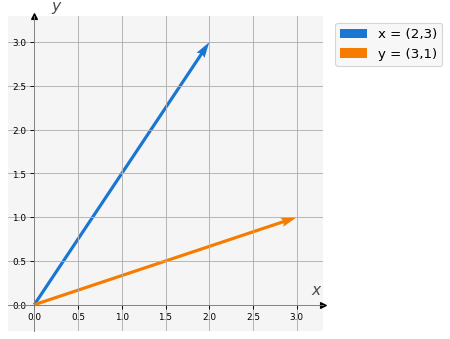
\includegraphics{02_precios_producto_files/figure-pdf/cell-4-output-1.png}

\textbf{Observaciones} * Los productos A y B han estado a la venta desde
2013 a 2019. * El producto C comenzó su venta en 2015, el D en 2016 y el
E en 2018. * El precio de A y B bajó en 2016, un año después de que
entró al mercado el producto C en 2015. Esta observación es importante.

\section{Construcción de la
historia}\label{construcciuxf3n-de-la-historia}

\subsection{El contexto: ¿Quién? ¿Qué?
¿Cómo?}\label{el-contexto-quiuxe9n-quuxe9-cuxf3mo}

\begin{itemize}
\item
  \textbf{¿Quién?} VP (Vice President of product), el que conoce todas
  las cuestiones técnicas del producto, el que hace la primera decisión
  para poner el precio. Es a quién se presentará el análisis de los
  datos.
\item
  \textbf{¿Qué?} Análisis de cómo el precio de los competidores ha
  cambiado con el tiempo y recomendar un rango de precios.
\item
  \textbf{¿Cómo?} Mostrar un precio promedio al menudeo de los productos
  A, B, C, D y E para diferentes años.
\end{itemize}

\subsubsection{La idea central}\label{la-idea-central}

\begin{itemize}
\tightlist
\item
  Articular un punto de vista único para transmitir lo que está en juego
  en un solo enunciado.
\item
  Para nuestro ejemplo diríamos algo como lo siguiente:

  \begin{itemize}
  \tightlist
  \item
    ``Con base en el análisis de precios del mercado y su cambio en el
    tiempo, para ser competitivos, se recomienda introducir nuestro
    producto a un precio al menudeo en el rango \(P - Q\).''
  \end{itemize}
\end{itemize}

\subsubsection{La historia en 3 minutos}\label{la-historia-en-3-minutos}

\begin{itemize}
\tightlist
\item
  Si solo tuvieras tres minutos para contar tu historia con palabras,
  ¿cómo lo harías?
\item
  Si eres capaz de hacer esto, significa que tienes muy claro lo que
  deseas contar.

  \begin{itemize}
  \tightlist
  \item
    Intenta hacer esto con tu historia.
  \item
    Grábate y escúchate varias veces.
  \item
    Repítelo hasta que sientas que lo has logrado.
  \end{itemize}
\item
  Tanto la idea central como la historia en 3 minutos, serán de utilidad
  para la presentación de tu historia.
\end{itemize}

\subsubsection{El color}\label{el-color}

\begin{itemize}
\tightlist
\item
  El color puede ayudar a discernir entre valores de datos; pero también
  puede confundir.
\item
  En esta visualización, los colores distraen del objetivo principal:
  ``mostrar el cambio en los precios a lo largo del tiempo''.
\item
  Entonces, la primera mejora es eliminar el color, vea la siguiente
  visualización.
\end{itemize}

\begin{Shaded}
\begin{Highlighting}[]
\CommentTok{\# Visualización 2: eliminamos el color}

\CommentTok{\# En la función plot() de DataFrame definimos el color}
\NormalTok{precios.plot(kind}\OperatorTok{=}\StringTok{\textquotesingle{}bar\textquotesingle{}}\NormalTok{, rot}\OperatorTok{=}\DecValTok{0}\NormalTok{, color}\OperatorTok{=}\StringTok{\textquotesingle{}gray\textquotesingle{}}\NormalTok{)}

\NormalTok{plt.yticks(ticks}\OperatorTok{=}\NormalTok{[}\DecValTok{0}\NormalTok{,}\DecValTok{100}\NormalTok{,}\DecValTok{200}\NormalTok{,}\DecValTok{300}\NormalTok{,}\DecValTok{400}\NormalTok{,}\DecValTok{500}\NormalTok{], labels}\OperatorTok{=}\NormalTok{[}\StringTok{\textquotesingle{}\textbackslash{}$0\textquotesingle{}}\NormalTok{,}\StringTok{\textquotesingle{}\textbackslash{}$100\textquotesingle{}}\NormalTok{,}\StringTok{\textquotesingle{}\textbackslash{}$200\textquotesingle{}}\NormalTok{,}\StringTok{\textquotesingle{}\textbackslash{}$300\textquotesingle{}}\NormalTok{,}\StringTok{\textquotesingle{}\textbackslash{}$400\textquotesingle{}}\NormalTok{,}\StringTok{\textquotesingle{}\textbackslash{}$500\textquotesingle{}}\NormalTok{])}
\NormalTok{plt.title(}\StringTok{\textquotesingle{}Los precios han bajado desde la introducción del producto C en 2015\textquotesingle{}}\NormalTok{, c}\OperatorTok{=}\StringTok{\textquotesingle{}blue\textquotesingle{}}\NormalTok{, y}\OperatorTok{=}\FloatTok{1.05}\NormalTok{)}
\NormalTok{plt.suptitle(}\StringTok{\textquotesingle{}Precio promedio por año\textquotesingle{}}\NormalTok{, fontsize}\OperatorTok{=}\DecValTok{24}\NormalTok{, y}\OperatorTok{=}\FloatTok{1.05}\NormalTok{)}
\NormalTok{plt.legend(loc}\OperatorTok{=}\StringTok{\textquotesingle{}lower center\textquotesingle{}}\NormalTok{, bbox\_to\_anchor}\OperatorTok{=}\NormalTok{(}\FloatTok{0.5}\NormalTok{, }\OperatorTok{{-}}\FloatTok{0.25}\NormalTok{), ncol}\OperatorTok{=}\DecValTok{7}\NormalTok{)}
\NormalTok{plt.grid(axis}\OperatorTok{=}\StringTok{\textquotesingle{}y\textquotesingle{}}\NormalTok{)}
\NormalTok{plt.show()}
\end{Highlighting}
\end{Shaded}

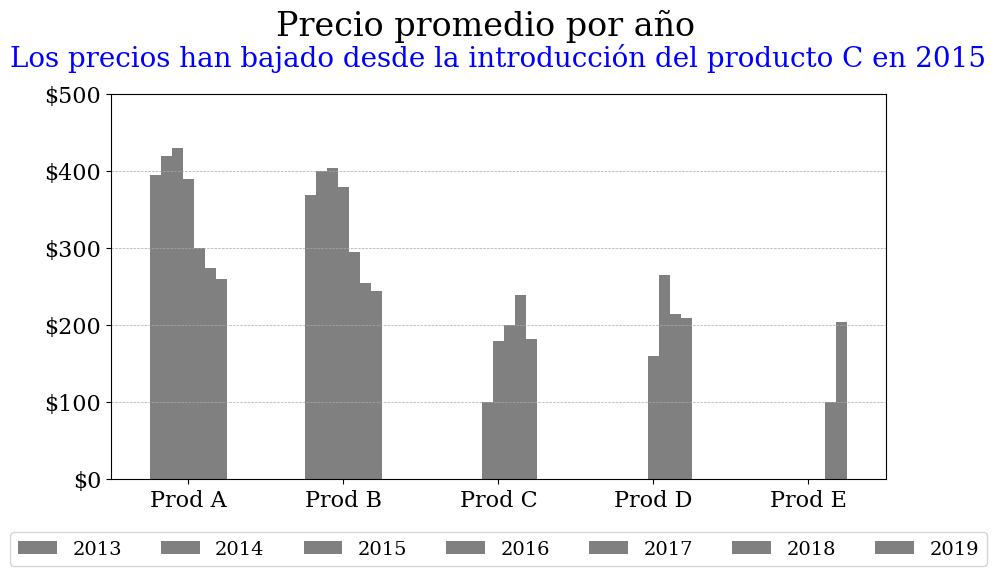
\includegraphics{02_precios_producto_files/figure-pdf/cell-5-output-1.png}

\textbf{Observaciones} - Efectivamente, el color ya no es un distractor,
sin embargo, no se distingue la información por años. - De acuerdo con
el texto de la primera visualización, vamos a resaltar la información a
partir del año 2015, que fue cuando se introdujo el producto C y los
precios empezaron a bajar.

\textbf{Gráfica de barras gris y negro}

\begin{Shaded}
\begin{Highlighting}[]
\NormalTok{precios.plot(y }\OperatorTok{=}\NormalTok{ [}\DecValTok{2013}\NormalTok{, }\DecValTok{2014}\NormalTok{], kind}\OperatorTok{=}\StringTok{\textquotesingle{}bar\textquotesingle{}}\NormalTok{, rot}\OperatorTok{=}\DecValTok{0}\NormalTok{, color}\OperatorTok{=}\StringTok{\textquotesingle{}gray\textquotesingle{}}\NormalTok{)}
\NormalTok{precios.plot(y }\OperatorTok{=}\NormalTok{ [}\DecValTok{2015}\NormalTok{, }\DecValTok{2016}\NormalTok{, }\DecValTok{2017}\NormalTok{, }\DecValTok{2018}\NormalTok{, }\DecValTok{2019}\NormalTok{], kind}\OperatorTok{=}\StringTok{\textquotesingle{}bar\textquotesingle{}}\NormalTok{, rot}\OperatorTok{=}\DecValTok{0}\NormalTok{, color}\OperatorTok{=}\StringTok{\textquotesingle{}k\textquotesingle{}}\NormalTok{)}
\end{Highlighting}
\end{Shaded}

\includegraphics{02_precios_producto_files/figure-pdf/cell-6-output-1.png}

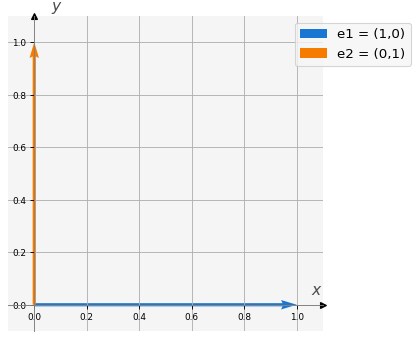
\includegraphics{02_precios_producto_files/figure-pdf/cell-6-output-2.png}

\textbf{Gráfica de barras gris y negro juntas}

\begin{Shaded}
\begin{Highlighting}[]
\CommentTok{\# Juntamos las dos gráficas en una sola}
\NormalTok{ax1 }\OperatorTok{=}\NormalTok{ precios.plot(y }\OperatorTok{=}\NormalTok{ [}\DecValTok{2013}\NormalTok{, }\DecValTok{2014}\NormalTok{], kind}\OperatorTok{=}\StringTok{\textquotesingle{}bar\textquotesingle{}}\NormalTok{, rot}\OperatorTok{=}\DecValTok{0}\NormalTok{, color}\OperatorTok{=}\StringTok{\textquotesingle{}gray\textquotesingle{}}\NormalTok{)}
\NormalTok{precios.plot(y }\OperatorTok{=}\NormalTok{ [}\DecValTok{2015}\NormalTok{, }\DecValTok{2016}\NormalTok{, }\DecValTok{2017}\NormalTok{, }\DecValTok{2018}\NormalTok{, }\DecValTok{2019}\NormalTok{], kind}\OperatorTok{=}\StringTok{\textquotesingle{}bar\textquotesingle{}}\NormalTok{, rot}\OperatorTok{=}\DecValTok{0}\NormalTok{, color}\OperatorTok{=}\StringTok{\textquotesingle{}k\textquotesingle{}}\NormalTok{, ax }\OperatorTok{=}\NormalTok{ ax1)}

\NormalTok{plt.yticks(ticks}\OperatorTok{=}\NormalTok{[}\DecValTok{0}\NormalTok{,}\DecValTok{100}\NormalTok{,}\DecValTok{200}\NormalTok{,}\DecValTok{300}\NormalTok{,}\DecValTok{400}\NormalTok{,}\DecValTok{500}\NormalTok{], labels}\OperatorTok{=}\NormalTok{[}\StringTok{\textquotesingle{}\textbackslash{}$0\textquotesingle{}}\NormalTok{,}\StringTok{\textquotesingle{}\textbackslash{}$100\textquotesingle{}}\NormalTok{,}\StringTok{\textquotesingle{}\textbackslash{}$200\textquotesingle{}}\NormalTok{,}\StringTok{\textquotesingle{}\textbackslash{}$300\textquotesingle{}}\NormalTok{,}\StringTok{\textquotesingle{}\textbackslash{}$400\textquotesingle{}}\NormalTok{,}\StringTok{\textquotesingle{}\textbackslash{}$500\textquotesingle{}}\NormalTok{])}
\NormalTok{plt.title(}\StringTok{\textquotesingle{}Los precios han bajado desde la introducción del producto C en 2015\textquotesingle{}}\NormalTok{, c}\OperatorTok{=}\StringTok{\textquotesingle{}blue\textquotesingle{}}\NormalTok{, y}\OperatorTok{=}\FloatTok{1.05}\NormalTok{)}
\NormalTok{plt.suptitle(}\StringTok{\textquotesingle{}Precio promedio por año\textquotesingle{}}\NormalTok{, fontsize}\OperatorTok{=}\DecValTok{24}\NormalTok{, y}\OperatorTok{=}\FloatTok{1.05}\NormalTok{)}
\NormalTok{plt.legend(loc}\OperatorTok{=}\StringTok{\textquotesingle{}lower center\textquotesingle{}}\NormalTok{, bbox\_to\_anchor}\OperatorTok{=}\NormalTok{(}\FloatTok{0.5}\NormalTok{, }\OperatorTok{{-}}\FloatTok{0.25}\NormalTok{), ncol}\OperatorTok{=}\DecValTok{7}\NormalTok{)}
\NormalTok{plt.grid(axis}\OperatorTok{=}\StringTok{\textquotesingle{}y\textquotesingle{}}\NormalTok{)}
\NormalTok{plt.show()}
\end{Highlighting}
\end{Shaded}

\includegraphics{02_precios_producto_files/figure-pdf/cell-7-output-1.png}

\textbf{Gráfica de barras gris y negras juntas, recorridas}

\begin{Shaded}
\begin{Highlighting}[]
\CommentTok{\# Visualización 3: resaltamos tendencias}

\CommentTok{\# Juntamos las dos gráficas en una sola y las colocamos una junto a otra}
\NormalTok{ax1 }\OperatorTok{=}\NormalTok{ precios.plot(y }\OperatorTok{=}\NormalTok{ [}\DecValTok{2013}\NormalTok{, }\DecValTok{2014}\NormalTok{], kind}\OperatorTok{=}\StringTok{\textquotesingle{}bar\textquotesingle{}}\NormalTok{, rot}\OperatorTok{=}\DecValTok{0}\NormalTok{, color}\OperatorTok{=}\StringTok{\textquotesingle{}gray\textquotesingle{}}\NormalTok{,}
\NormalTok{                  width}\OperatorTok{=}\FloatTok{0.2}\NormalTok{, position}\OperatorTok{=}\FloatTok{2.28}\NormalTok{)}
\NormalTok{precios.plot(y }\OperatorTok{=}\NormalTok{ [}\DecValTok{2015}\NormalTok{, }\DecValTok{2016}\NormalTok{, }\DecValTok{2017}\NormalTok{, }\DecValTok{2018}\NormalTok{, }\DecValTok{2019}\NormalTok{], kind}\OperatorTok{=}\StringTok{\textquotesingle{}bar\textquotesingle{}}\NormalTok{, rot}\OperatorTok{=}\DecValTok{0}\NormalTok{, color}\OperatorTok{=}\StringTok{\textquotesingle{}k\textquotesingle{}}\NormalTok{, }
\NormalTok{             ax }\OperatorTok{=}\NormalTok{ ax1)}

\NormalTok{plt.yticks(ticks}\OperatorTok{=}\NormalTok{[}\DecValTok{0}\NormalTok{,}\DecValTok{100}\NormalTok{,}\DecValTok{200}\NormalTok{,}\DecValTok{300}\NormalTok{,}\DecValTok{400}\NormalTok{,}\DecValTok{500}\NormalTok{], labels}\OperatorTok{=}\NormalTok{[}\StringTok{\textquotesingle{}\textbackslash{}$0\textquotesingle{}}\NormalTok{,}\StringTok{\textquotesingle{}\textbackslash{}$100\textquotesingle{}}\NormalTok{,}\StringTok{\textquotesingle{}\textbackslash{}$200\textquotesingle{}}\NormalTok{,}\StringTok{\textquotesingle{}\textbackslash{}$300\textquotesingle{}}\NormalTok{,}\StringTok{\textquotesingle{}\textbackslash{}$400\textquotesingle{}}\NormalTok{,}\StringTok{\textquotesingle{}\textbackslash{}$500\textquotesingle{}}\NormalTok{])}
\NormalTok{plt.title(}\StringTok{\textquotesingle{}Los precios han bajado desde la introducción del producto C en 2015\textquotesingle{}}\NormalTok{, c}\OperatorTok{=}\StringTok{\textquotesingle{}blue\textquotesingle{}}\NormalTok{, y}\OperatorTok{=}\FloatTok{1.05}\NormalTok{)}
\NormalTok{plt.suptitle(}\StringTok{\textquotesingle{}Precio promedio por año\textquotesingle{}}\NormalTok{, fontsize}\OperatorTok{=}\DecValTok{24}\NormalTok{, y}\OperatorTok{=}\FloatTok{1.05}\NormalTok{)}
\NormalTok{plt.legend(loc}\OperatorTok{=}\StringTok{\textquotesingle{}lower center\textquotesingle{}}\NormalTok{, bbox\_to\_anchor}\OperatorTok{=}\NormalTok{(}\FloatTok{0.5}\NormalTok{, }\OperatorTok{{-}}\FloatTok{0.25}\NormalTok{), ncol}\OperatorTok{=}\DecValTok{7}\NormalTok{)}
\NormalTok{plt.grid(axis}\OperatorTok{=}\StringTok{\textquotesingle{}y\textquotesingle{}}\NormalTok{)}
\NormalTok{plt.show()}
\end{Highlighting}
\end{Shaded}

\includegraphics{02_precios_producto_files/figure-pdf/cell-8-output-1.png}

\textbf{Observaciones} - Se nota claramente como los precios de A y de B
van en declive después de 2015. - Pero no pasa lo mismo con los
productos D y E, que fueron lanzados en años posteriores a C. - Por lo
tanto, el texto en azul de la gráfica, no es correcto. Ese texto debe
ser corregido en la visualización final.

\subsection{Eligiendo la estrategia de
visualización}\label{eligiendo-la-estrategia-de-visualizaciuxf3n}

\begin{itemize}
\tightlist
\item
  Parece que la forma en que se está visualizando la información no es
  la más adecuada.
\item
  Se desea mostrar cómo cambia un precio a lo largo del tiempo y tratar
  de encontrar una tendencia.
\item
  Es posible que usar líneas sea lo más adecuado.
\item
  Adicionalmente, las líneas eliminan el efecto de escalera que se ve en
  las barras.
\end{itemize}

\textbf{Gráfica de líneas con DataFrame}

\begin{Shaded}
\begin{Highlighting}[]
\NormalTok{precios.plot(kind}\OperatorTok{=}\StringTok{\textquotesingle{}line\textquotesingle{}}\NormalTok{, rot}\OperatorTok{=}\DecValTok{0}\NormalTok{)}

\NormalTok{plt.yticks(ticks}\OperatorTok{=}\NormalTok{[}\DecValTok{0}\NormalTok{,}\DecValTok{100}\NormalTok{,}\DecValTok{200}\NormalTok{,}\DecValTok{300}\NormalTok{,}\DecValTok{400}\NormalTok{,}\DecValTok{500}\NormalTok{], }
\NormalTok{           labels}\OperatorTok{=}\NormalTok{[}\StringTok{\textquotesingle{}\textbackslash{}$0\textquotesingle{}}\NormalTok{,}\StringTok{\textquotesingle{}\textbackslash{}$100\textquotesingle{}}\NormalTok{,}\StringTok{\textquotesingle{}\textbackslash{}$200\textquotesingle{}}\NormalTok{,}\StringTok{\textquotesingle{}\textbackslash{}$300\textquotesingle{}}\NormalTok{,}\StringTok{\textquotesingle{}\textbackslash{}$400\textquotesingle{}}\NormalTok{,}\StringTok{\textquotesingle{}\textbackslash{}$500\textquotesingle{}}\NormalTok{])}
\NormalTok{plt.title(}\StringTok{\textquotesingle{}Los precios han bajado desde la introducción del producto C en 2015\textquotesingle{}}\NormalTok{, c}\OperatorTok{=}\StringTok{\textquotesingle{}blue\textquotesingle{}}\NormalTok{, y}\OperatorTok{=}\FloatTok{1.05}\NormalTok{)}
\NormalTok{plt.suptitle(}\StringTok{\textquotesingle{}Precio promedio por año\textquotesingle{}}\NormalTok{, fontsize}\OperatorTok{=}\DecValTok{24}\NormalTok{, y}\OperatorTok{=}\FloatTok{1.05}\NormalTok{)}
\NormalTok{plt.legend(loc}\OperatorTok{=}\StringTok{\textquotesingle{}lower center\textquotesingle{}}\NormalTok{, bbox\_to\_anchor}\OperatorTok{=}\NormalTok{(}\FloatTok{0.5}\NormalTok{, }\OperatorTok{{-}}\FloatTok{0.25}\NormalTok{), ncol}\OperatorTok{=}\DecValTok{7}\NormalTok{)}
\NormalTok{plt.grid(axis}\OperatorTok{=}\StringTok{\textquotesingle{}y\textquotesingle{}}\NormalTok{)}
\NormalTok{plt.show()}
\end{Highlighting}
\end{Shaded}

\includegraphics{02_precios_producto_files/figure-pdf/cell-9-output-1.png}

Observa que las líneas, como se graficaron antes, no dan mucha
información y por le contrario se ve todo enmarañado.

Vamos a usar Matplotlib en lo que sigue para tener acceso a más
funcionalidades.

\subsubsection{Líneas por cada
producto}\label{luxedneas-por-cada-producto}

Primero arreglamos los datos por producto (renglones del DataFrame)

\begin{Shaded}
\begin{Highlighting}[]
\NormalTok{A }\OperatorTok{=}\NormalTok{ np.array(precios.iloc[}\DecValTok{0}\NormalTok{])}
\NormalTok{B }\OperatorTok{=}\NormalTok{ np.array(precios.iloc[}\DecValTok{1}\NormalTok{])}
\NormalTok{C }\OperatorTok{=}\NormalTok{ np.array(precios.iloc[}\DecValTok{2}\NormalTok{])}
\NormalTok{D }\OperatorTok{=}\NormalTok{ np.array(precios.iloc[}\DecValTok{3}\NormalTok{])}
\NormalTok{E }\OperatorTok{=}\NormalTok{ np.array(precios.iloc[}\DecValTok{4}\NormalTok{])}
\BuiltInTok{print}\NormalTok{(A)}
\BuiltInTok{print}\NormalTok{(B)}
\BuiltInTok{print}\NormalTok{(C)}
\BuiltInTok{print}\NormalTok{(D)}
\BuiltInTok{print}\NormalTok{(E)}
\end{Highlighting}
\end{Shaded}

\begin{verbatim}
[395. 420. 430. 390. 300. 275. 260.]
[370. 400. 405. 380. 295. 255. 245.]
[ nan  nan 100. 180. 200. 240. 182.]
[ nan  nan  nan 160. 265. 215. 210.]
[ nan  nan  nan  nan  nan 100. 205.]
\end{verbatim}

\begin{Shaded}
\begin{Highlighting}[]
\CommentTok{\# Arreglo para usarse en el eje x}
\NormalTok{x }\OperatorTok{=}\NormalTok{ np.array([i }\ControlFlowTok{for}\NormalTok{ i }\KeywordTok{in} \BuiltInTok{range}\NormalTok{(}\DecValTok{7}\NormalTok{)])}
\BuiltInTok{print}\NormalTok{(}\StringTok{\textquotesingle{}}\CharTok{\textbackslash{}n}\StringTok{x: \textquotesingle{}}\NormalTok{,x)}
\end{Highlighting}
\end{Shaded}

\begin{verbatim}

x:  [0 1 2 3 4 5 6]
\end{verbatim}

\textbf{Graficamos barras y líneas}

\begin{Shaded}
\begin{Highlighting}[]
\CommentTok{\# Un primer intento}
\NormalTok{fig }\OperatorTok{=}\NormalTok{ plt.figure() }\CommentTok{\# Se define una figura}
\NormalTok{ax }\OperatorTok{=}\NormalTok{ fig.gca()     }\CommentTok{\# Se obtienen los ejes de la figura}

\CommentTok{\# Producto A}
\NormalTok{ax.bar(x, A)}
\NormalTok{ax.plot(x, A, lw}\OperatorTok{=}\DecValTok{3}\NormalTok{, c}\OperatorTok{=}\StringTok{\textquotesingle{}k\textquotesingle{}}\NormalTok{)}

\NormalTok{plt.show()}
\end{Highlighting}
\end{Shaded}

\includegraphics{02_precios_producto_files/figure-pdf/cell-12-output-1.png}

\begin{Shaded}
\begin{Highlighting}[]
\CommentTok{\# Visualización 4: usamos barras y líneas}
\NormalTok{fig }\OperatorTok{=}\NormalTok{ plt.figure() }\CommentTok{\# Se define una figura}
\NormalTok{ax }\OperatorTok{=}\NormalTok{ fig.gca()     }\CommentTok{\# Se obtienen los ejes de la figura}

\NormalTok{offset }\OperatorTok{=} \DecValTok{10} \CommentTok{\# Este número nos ayudará a recorrer las gráficas}

\CommentTok{\# Producto A}
\NormalTok{ax.bar(x, A, color}\OperatorTok{=}\StringTok{\textquotesingle{}silver\textquotesingle{}}\NormalTok{)}
\NormalTok{ax.plot(x, A, lw}\OperatorTok{=}\DecValTok{3}\NormalTok{, c}\OperatorTok{=}\StringTok{\textquotesingle{}k\textquotesingle{}}\NormalTok{)}
\NormalTok{ax.text(}\OperatorTok{{-}}\FloatTok{0.5}\NormalTok{,}\DecValTok{410}\NormalTok{,}\StringTok{\textquotesingle{}2013\textquotesingle{}}\NormalTok{, fontsize}\OperatorTok{=}\DecValTok{10}\NormalTok{, color}\OperatorTok{=}\StringTok{\textquotesingle{}k\textquotesingle{}}\NormalTok{, rotation}\OperatorTok{=}\StringTok{\textquotesingle{}vertical\textquotesingle{}}\NormalTok{)}
\NormalTok{ax.text(}\FloatTok{5.75}\NormalTok{,}\DecValTok{270}\NormalTok{,}\StringTok{\textquotesingle{}2019\textquotesingle{}}\NormalTok{, fontsize}\OperatorTok{=}\DecValTok{10}\NormalTok{, color}\OperatorTok{=}\StringTok{\textquotesingle{}k\textquotesingle{}}\NormalTok{, rotation}\OperatorTok{=}\StringTok{\textquotesingle{}vertical\textquotesingle{}}\NormalTok{)}

\CommentTok{\# Producto B}
\NormalTok{ax.bar(x}\OperatorTok{+}\NormalTok{offset, B, color}\OperatorTok{=}\StringTok{\textquotesingle{}silver\textquotesingle{}}\NormalTok{)}
\NormalTok{ax.plot(x}\OperatorTok{+}\NormalTok{offset, B, lw}\OperatorTok{=}\DecValTok{3}\NormalTok{, c}\OperatorTok{=}\StringTok{\textquotesingle{}k\textquotesingle{}}\NormalTok{)}

\CommentTok{\# Producto C}
\NormalTok{ax.bar(x}\OperatorTok{+}\DecValTok{2}\OperatorTok{*}\NormalTok{offset}\OperatorTok{{-}}\DecValTok{2}\NormalTok{, C, color}\OperatorTok{=}\StringTok{\textquotesingle{}silver\textquotesingle{}}\NormalTok{)}
\NormalTok{ax.plot(x}\OperatorTok{+}\DecValTok{2}\OperatorTok{*}\NormalTok{offset}\OperatorTok{{-}}\DecValTok{2}\NormalTok{, C, lw}\OperatorTok{=}\DecValTok{3}\NormalTok{, c}\OperatorTok{=}\StringTok{\textquotesingle{}k\textquotesingle{}}\NormalTok{)}

\CommentTok{\# Producto D}
\NormalTok{ax.bar(x}\OperatorTok{+}\DecValTok{3}\OperatorTok{*}\NormalTok{offset}\OperatorTok{{-}}\DecValTok{3}\NormalTok{, D, color}\OperatorTok{=}\StringTok{\textquotesingle{}silver\textquotesingle{}}\NormalTok{)}
\NormalTok{ax.plot(x}\OperatorTok{+}\DecValTok{3}\OperatorTok{*}\NormalTok{offset}\OperatorTok{{-}}\DecValTok{3}\NormalTok{, D, lw}\OperatorTok{=}\DecValTok{3}\NormalTok{, c}\OperatorTok{=}\StringTok{\textquotesingle{}k\textquotesingle{}}\NormalTok{)}

\CommentTok{\# Producto E}
\NormalTok{ax.bar(x}\OperatorTok{+}\DecValTok{4}\OperatorTok{*}\NormalTok{offset}\OperatorTok{{-}}\DecValTok{5}\NormalTok{, E, color}\OperatorTok{=}\StringTok{\textquotesingle{}silver\textquotesingle{}}\NormalTok{)}
\NormalTok{ax.plot(x}\OperatorTok{+}\DecValTok{4}\OperatorTok{*}\NormalTok{offset}\OperatorTok{{-}}\DecValTok{5}\NormalTok{, E, lw}\OperatorTok{=}\DecValTok{3}\NormalTok{, c}\OperatorTok{=}\StringTok{\textquotesingle{}k\textquotesingle{}}\NormalTok{)}

\CommentTok{\# Etiquetas de los ejes}
\NormalTok{ax.set\_ylabel(}\StringTok{\textquotesingle{}Precio del producto\textquotesingle{}}\NormalTok{, fontsize}\OperatorTok{=}\DecValTok{15}\NormalTok{)}
\NormalTok{ax.set\_xlabel(}\StringTok{\textquotesingle{}Año\textquotesingle{}}\NormalTok{, fontsize}\OperatorTok{=}\DecValTok{15}\NormalTok{)}

\CommentTok{\# Marcas sobre los ejes}
\NormalTok{ax.set\_xticks(ticks}\OperatorTok{=}\NormalTok{[}\DecValTok{3}\NormalTok{, offset}\OperatorTok{+}\DecValTok{3}\NormalTok{, }\DecValTok{2}\OperatorTok{*}\NormalTok{offset}\OperatorTok{+}\DecValTok{2}\NormalTok{, }\DecValTok{3}\OperatorTok{*}\NormalTok{offset}\OperatorTok{+}\DecValTok{1}\NormalTok{, }\DecValTok{4}\OperatorTok{*}\NormalTok{offset], }
\NormalTok{              labels}\OperatorTok{=}\NormalTok{[}\StringTok{\textquotesingle{}Prod A\textquotesingle{}}\NormalTok{, }\StringTok{\textquotesingle{}Prod B\textquotesingle{}}\NormalTok{, }\StringTok{\textquotesingle{}Prod C\textquotesingle{}}\NormalTok{, }\StringTok{\textquotesingle{}Prod D\textquotesingle{}}\NormalTok{, }\StringTok{\textquotesingle{}Prod E\textquotesingle{}}\NormalTok{])}
\NormalTok{ax.set\_yticks(ticks}\OperatorTok{=}\NormalTok{[}\DecValTok{0}\NormalTok{,}\DecValTok{100}\NormalTok{,}\DecValTok{200}\NormalTok{,}\DecValTok{300}\NormalTok{,}\DecValTok{400}\NormalTok{,}\DecValTok{500}\NormalTok{], }
\NormalTok{              labels}\OperatorTok{=}\NormalTok{[}\StringTok{\textquotesingle{}\textbackslash{}$0\textquotesingle{}}\NormalTok{,}\StringTok{\textquotesingle{}\textbackslash{}$100\textquotesingle{}}\NormalTok{,}\StringTok{\textquotesingle{}\textbackslash{}$200\textquotesingle{}}\NormalTok{,}\StringTok{\textquotesingle{}\textbackslash{}$300\textquotesingle{}}\NormalTok{,}\StringTok{\textquotesingle{}\textbackslash{}$400\textquotesingle{}}\NormalTok{,}\StringTok{\textquotesingle{}\textbackslash{}$500\textquotesingle{}}\NormalTok{])}

\CommentTok{\# Rejilla en el eje y}
\NormalTok{ax.grid(axis}\OperatorTok{=}\StringTok{\textquotesingle{}y\textquotesingle{}}\NormalTok{)}

\NormalTok{plt.title(}\StringTok{\textquotesingle{}Los precios han bajado desde la introducción del producto C en 2015\textquotesingle{}}\NormalTok{, c}\OperatorTok{=}\StringTok{\textquotesingle{}blue\textquotesingle{}}\NormalTok{, y}\OperatorTok{=}\FloatTok{1.05}\NormalTok{)}
\NormalTok{plt.suptitle(}\StringTok{\textquotesingle{}Precio promedio por año\textquotesingle{}}\NormalTok{, fontsize}\OperatorTok{=}\DecValTok{24}\NormalTok{, y}\OperatorTok{=}\FloatTok{1.05}\NormalTok{)}
\NormalTok{plt.show()}
\end{Highlighting}
\end{Shaded}

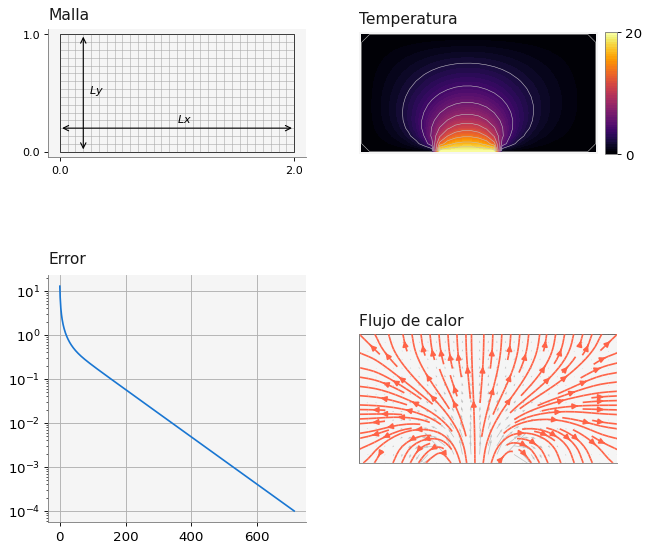
\includegraphics{02_precios_producto_files/figure-pdf/cell-13-output-1.png}

\textbf{Observaciones}

\begin{itemize}
\tightlist
\item
  Se usa el mismo diseño (ejes, límites, título, \ldots)
\item
  Esta visualización permite ver con más claridad lo que sucede con el
  precio de cada producto a lo largo del tiempo.
\item
  Aunque es difícil comparar entre productos.
\item
  Si graficamos en un mismo eje \(x\) todos los productos obtenemos algo
  mejor.
\end{itemize}

\subsubsection{Líneas en un mismo
eje.}\label{luxedneas-en-un-mismo-eje.}

\begin{Shaded}
\begin{Highlighting}[]
\NormalTok{x2 }\OperatorTok{=}\NormalTok{ np.arange(}\DecValTok{2013}\NormalTok{,}\DecValTok{2020}\NormalTok{,}\DecValTok{1}\NormalTok{)}
\NormalTok{x2}
\end{Highlighting}
\end{Shaded}

\begin{verbatim}
array([2013, 2014, 2015, 2016, 2017, 2018, 2019])
\end{verbatim}

\begin{Shaded}
\begin{Highlighting}[]
\CommentTok{\# Visualización 5: usamos solo líneas }
\NormalTok{fig }\OperatorTok{=}\NormalTok{ plt.figure() }\CommentTok{\# Se define una figura}
\NormalTok{ax }\OperatorTok{=}\NormalTok{ fig.gca()     }\CommentTok{\# Se obtienen los ejes de la figura}

\CommentTok{\# Producto A}
\NormalTok{ax.plot(x2, A, lw}\OperatorTok{=}\DecValTok{3}\NormalTok{, c}\OperatorTok{=}\StringTok{\textquotesingle{}k\textquotesingle{}}\NormalTok{)}

\CommentTok{\# Producto B}
\NormalTok{ax.plot(x2, B, lw}\OperatorTok{=}\DecValTok{3}\NormalTok{, c}\OperatorTok{=}\StringTok{\textquotesingle{}k\textquotesingle{}}\NormalTok{)}

\CommentTok{\# Producto C}
\NormalTok{ax.plot(x2, C, lw}\OperatorTok{=}\DecValTok{3}\NormalTok{, c}\OperatorTok{=}\StringTok{\textquotesingle{}k\textquotesingle{}}\NormalTok{)}

\CommentTok{\# Producto D}
\NormalTok{ax.plot(x2, D, lw}\OperatorTok{=}\DecValTok{3}\NormalTok{, c}\OperatorTok{=}\StringTok{\textquotesingle{}k\textquotesingle{}}\NormalTok{)}

\CommentTok{\# Producto E}
\NormalTok{ax.plot(x2, E, lw}\OperatorTok{=}\DecValTok{3}\NormalTok{, c}\OperatorTok{=}\StringTok{\textquotesingle{}k\textquotesingle{}}\NormalTok{)}

\CommentTok{\# Etiquetas de los ejes}
\NormalTok{ax.set\_ylabel(}\StringTok{\textquotesingle{}Precio del producto\textquotesingle{}}\NormalTok{, fontsize}\OperatorTok{=}\DecValTok{15}\NormalTok{)}
\NormalTok{ax.set\_xlabel(}\StringTok{\textquotesingle{}Año\textquotesingle{}}\NormalTok{, fontsize}\OperatorTok{=}\DecValTok{15}\NormalTok{)}

\CommentTok{\# Límites en los ejes}
\NormalTok{ax.set\_ylim(}\DecValTok{0}\NormalTok{,}\DecValTok{500}\NormalTok{)}
\NormalTok{ax.set\_xlim(}\FloatTok{2012.5}\NormalTok{,}\FloatTok{2019.5}\NormalTok{)}

\CommentTok{\# Marcas sobre los ejes}
\NormalTok{ax.set\_xticks(ticks}\OperatorTok{=}\NormalTok{[i }\ControlFlowTok{for}\NormalTok{ i }\KeywordTok{in} \BuiltInTok{range}\NormalTok{(}\DecValTok{2013}\NormalTok{,}\DecValTok{2020}\NormalTok{)])}
\NormalTok{ax.set\_yticks(ticks}\OperatorTok{=}\NormalTok{[}\DecValTok{0}\NormalTok{,}\DecValTok{100}\NormalTok{,}\DecValTok{200}\NormalTok{,}\DecValTok{300}\NormalTok{,}\DecValTok{400}\NormalTok{,}\DecValTok{500}\NormalTok{], }
\NormalTok{              labels}\OperatorTok{=}\NormalTok{[}\StringTok{\textquotesingle{}\textbackslash{}$0\textquotesingle{}}\NormalTok{,}\StringTok{\textquotesingle{}\textbackslash{}$100\textquotesingle{}}\NormalTok{,}\StringTok{\textquotesingle{}\textbackslash{}$200\textquotesingle{}}\NormalTok{,}\StringTok{\textquotesingle{}\textbackslash{}$300\textquotesingle{}}\NormalTok{,}\StringTok{\textquotesingle{}\textbackslash{}$400\textquotesingle{}}\NormalTok{,}\StringTok{\textquotesingle{}\textbackslash{}$500\textquotesingle{}}\NormalTok{])}

\CommentTok{\# Rejilla }
\NormalTok{ax.grid()}

\NormalTok{plt.title(}\StringTok{\textquotesingle{}Los precios han bajado desde la introducción del producto C en 2015\textquotesingle{}}\NormalTok{, c}\OperatorTok{=}\StringTok{\textquotesingle{}blue\textquotesingle{}}\NormalTok{, y}\OperatorTok{=}\FloatTok{1.05}\NormalTok{)}
\NormalTok{plt.suptitle(}\StringTok{\textquotesingle{}Precio promedio por año\textquotesingle{}}\NormalTok{, fontsize}\OperatorTok{=}\DecValTok{24}\NormalTok{, y}\OperatorTok{=}\FloatTok{1.05}\NormalTok{)}
\NormalTok{plt.show()}
\end{Highlighting}
\end{Shaded}

\includegraphics{02_precios_producto_files/figure-pdf/cell-15-output-1.png}

\textbf{Observaciones} - Obsérvese que se reduce el desorden y se evita
la repetición de etiquetas en las gráficas. - Quizá ahora podamos
agregar color (el cual habíamos eliminado antes) para identificar cada
producto.

\subsubsection{Líneas con color}\label{luxedneas-con-color}

\begin{Shaded}
\begin{Highlighting}[]
\CommentTok{\# Visualización 6: usamos líneas con color}
\NormalTok{fig }\OperatorTok{=}\NormalTok{ plt.figure() }\CommentTok{\# Se define una figura}
\NormalTok{ax }\OperatorTok{=}\NormalTok{ fig.gca()     }\CommentTok{\# Se obtienen los ejes de la figura}

\CommentTok{\# Producto A}
\NormalTok{ax.plot(x2, A, lw}\OperatorTok{=}\DecValTok{3}\NormalTok{, label}\OperatorTok{=}\StringTok{\textquotesingle{}Prod A\textquotesingle{}}\NormalTok{)}

\CommentTok{\# Producto B}
\NormalTok{ax.plot(x2, B, lw}\OperatorTok{=}\DecValTok{3}\NormalTok{, label}\OperatorTok{=}\StringTok{\textquotesingle{}Prod B\textquotesingle{}}\NormalTok{)}

\CommentTok{\# Producto C}
\NormalTok{ax.plot(x2, C, lw}\OperatorTok{=}\DecValTok{3}\NormalTok{, label}\OperatorTok{=}\StringTok{\textquotesingle{}Prod C\textquotesingle{}}\NormalTok{)}

\CommentTok{\# Producto D}
\NormalTok{ax.plot(x2, D, lw}\OperatorTok{=}\DecValTok{3}\NormalTok{, label}\OperatorTok{=}\StringTok{\textquotesingle{}Prod D\textquotesingle{}}\NormalTok{)}

\CommentTok{\# Producto E}
\NormalTok{ax.plot(x2, E, lw}\OperatorTok{=}\DecValTok{3}\NormalTok{, label}\OperatorTok{=}\StringTok{\textquotesingle{}Prod E\textquotesingle{}}\NormalTok{)}

\CommentTok{\# Etiquetas de los ejes}
\NormalTok{ax.set\_ylabel(}\StringTok{\textquotesingle{}Precio del producto\textquotesingle{}}\NormalTok{, fontsize}\OperatorTok{=}\DecValTok{15}\NormalTok{)}
\NormalTok{ax.set\_xlabel(}\StringTok{\textquotesingle{}Año\textquotesingle{}}\NormalTok{, fontsize}\OperatorTok{=}\DecValTok{15}\NormalTok{)}

\CommentTok{\# Límites en los ejes}
\NormalTok{ax.set\_ylim(}\DecValTok{0}\NormalTok{,}\DecValTok{500}\NormalTok{)}
\NormalTok{ax.set\_xlim(}\FloatTok{2012.5}\NormalTok{,}\FloatTok{2019.5}\NormalTok{)}

\CommentTok{\# Marcas sobre los ejes}
\NormalTok{ax.set\_xticks(ticks}\OperatorTok{=}\NormalTok{[i }\ControlFlowTok{for}\NormalTok{ i }\KeywordTok{in} \BuiltInTok{range}\NormalTok{(}\DecValTok{2013}\NormalTok{,}\DecValTok{2020}\NormalTok{)])}
\NormalTok{ax.set\_yticks(ticks}\OperatorTok{=}\NormalTok{[}\DecValTok{0}\NormalTok{,}\DecValTok{100}\NormalTok{,}\DecValTok{200}\NormalTok{,}\DecValTok{300}\NormalTok{,}\DecValTok{400}\NormalTok{,}\DecValTok{500}\NormalTok{], }
\NormalTok{              labels}\OperatorTok{=}\NormalTok{[}\StringTok{\textquotesingle{}\textbackslash{}$0\textquotesingle{}}\NormalTok{,}\StringTok{\textquotesingle{}\textbackslash{}$100\textquotesingle{}}\NormalTok{,}\StringTok{\textquotesingle{}\textbackslash{}$200\textquotesingle{}}\NormalTok{,}\StringTok{\textquotesingle{}\textbackslash{}$300\textquotesingle{}}\NormalTok{,}\StringTok{\textquotesingle{}\textbackslash{}$400\textquotesingle{}}\NormalTok{,}\StringTok{\textquotesingle{}\textbackslash{}$500\textquotesingle{}}\NormalTok{])}

\CommentTok{\# Rejilla }
\NormalTok{ax.grid()}

\NormalTok{plt.title(}\StringTok{\textquotesingle{}Los precios han bajado desde la introducción del producto C en 2015\textquotesingle{}}\NormalTok{, c}\OperatorTok{=}\StringTok{\textquotesingle{}blue\textquotesingle{}}\NormalTok{, y}\OperatorTok{=}\FloatTok{1.05}\NormalTok{)}
\NormalTok{plt.suptitle(}\StringTok{\textquotesingle{}Precio promedio por año\textquotesingle{}}\NormalTok{, fontsize}\OperatorTok{=}\DecValTok{24}\NormalTok{, y}\OperatorTok{=}\FloatTok{1.05}\NormalTok{)}
\NormalTok{plt.legend(loc}\OperatorTok{=}\StringTok{\textquotesingle{}lower center\textquotesingle{}}\NormalTok{, bbox\_to\_anchor}\OperatorTok{=}\NormalTok{(}\FloatTok{0.5}\NormalTok{, }\OperatorTok{{-}}\FloatTok{0.30}\NormalTok{), ncol}\OperatorTok{=}\DecValTok{7}\NormalTok{)}
\NormalTok{plt.show()}
\end{Highlighting}
\end{Shaded}

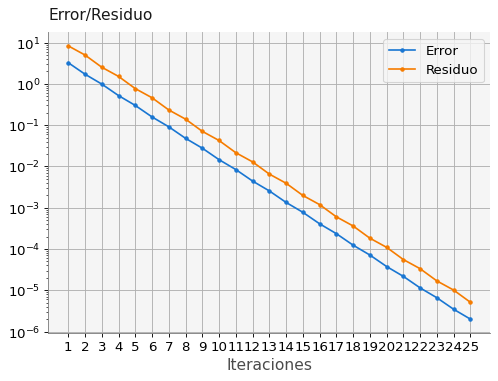
\includegraphics{02_precios_producto_files/figure-pdf/cell-16-output-1.png}

\subsection{Eliminando el desorden}\label{eliminando-el-desorden}

\begin{itemize}
\tightlist
\item
  Significa eliminar lo que no aporta información. En nuestro ejemplo
  podemos hacer lo siguiente:

  \begin{itemize}
  \tightlist
  \item
    Quitar protagonismo al título, debe estar, pero no debe distraer del
    objetivo principal; en este caso no necesita estar en texto
    resaltado (bold).
  \item
    Eliminar los bordes de la gráfica y la rejilla.
  \item
    Quitar protagonismo a los ejes y sus etiquetas haciéndolas más
    tenues.
  \item
    En este caso no es necesario poner la etiqueta a cada eje, pues de
    la información se deduce de que se trata.
  \item
    Eliminar el color otra vez; se puede usar de manera estratégica; más
    adelante se verá cómo.
  \item
    Etiquetar las líneas directamente. Esto evita el trabajo visual de
    la audiencia: ya no tiene que ver primero la leyenda, luego buscar
    en el gráfico la curva que corresponda, y esto varias veces hasta
    entender lo que se muestra.
  \end{itemize}
\end{itemize}

\begin{Shaded}
\begin{Highlighting}[]
\CommentTok{\# Visualización 7: eliminamos elementos que solo distraen}
\NormalTok{fig }\OperatorTok{=}\NormalTok{ plt.figure() }\CommentTok{\# Se define una figura}
\NormalTok{ax }\OperatorTok{=}\NormalTok{ fig.gca()     }\CommentTok{\# Se obtienen los ejes de la figura}

\CommentTok{\# Producto A}
\NormalTok{ax.plot(x2, A, lw}\OperatorTok{=}\DecValTok{3}\NormalTok{, c}\OperatorTok{=}\StringTok{\textquotesingle{}darkgray\textquotesingle{}}\NormalTok{)}

\CommentTok{\# Producto B}
\NormalTok{ax.plot(x2, B, lw}\OperatorTok{=}\DecValTok{3}\NormalTok{, c}\OperatorTok{=}\StringTok{\textquotesingle{}darkgray\textquotesingle{}}\NormalTok{)}

\CommentTok{\# Producto C}
\NormalTok{ax.plot(x2, C, lw}\OperatorTok{=}\DecValTok{3}\NormalTok{, c}\OperatorTok{=}\StringTok{\textquotesingle{}darkgray\textquotesingle{}}\NormalTok{)}

\CommentTok{\# Producto D}
\NormalTok{ax.plot(x2, D, lw}\OperatorTok{=}\DecValTok{3}\NormalTok{, c}\OperatorTok{=}\StringTok{\textquotesingle{}darkgray\textquotesingle{}}\NormalTok{)}

\CommentTok{\# Producto E}
\NormalTok{ax.plot(x2, E, lw}\OperatorTok{=}\DecValTok{3}\NormalTok{, c}\OperatorTok{=}\StringTok{\textquotesingle{}darkgray\textquotesingle{}}\NormalTok{)}

\CommentTok{\# Límites en los ejes}
\NormalTok{ax.set\_ylim(}\DecValTok{0}\NormalTok{,}\DecValTok{500}\NormalTok{)}
\NormalTok{ax.set\_xlim(}\FloatTok{2012.5}\NormalTok{,}\FloatTok{2019.5}\NormalTok{)}

\CommentTok{\# Marcas sobre los ejes}
\NormalTok{ax.set\_xticks(ticks}\OperatorTok{=}\NormalTok{[i }\ControlFlowTok{for}\NormalTok{ i }\KeywordTok{in} \BuiltInTok{range}\NormalTok{(}\DecValTok{2013}\NormalTok{,}\DecValTok{2020}\NormalTok{)])}
\NormalTok{ax.set\_yticks(ticks}\OperatorTok{=}\NormalTok{[}\DecValTok{0}\NormalTok{,}\DecValTok{100}\NormalTok{,}\DecValTok{200}\NormalTok{,}\DecValTok{300}\NormalTok{,}\DecValTok{400}\NormalTok{,}\DecValTok{500}\NormalTok{], }
\NormalTok{              labels}\OperatorTok{=}\NormalTok{[}\StringTok{\textquotesingle{}\textbackslash{}$0\textquotesingle{}}\NormalTok{,}\StringTok{\textquotesingle{}\textbackslash{}$100\textquotesingle{}}\NormalTok{,}\StringTok{\textquotesingle{}\textbackslash{}$200\textquotesingle{}}\NormalTok{,}\StringTok{\textquotesingle{}\textbackslash{}$300\textquotesingle{}}\NormalTok{,}\StringTok{\textquotesingle{}\textbackslash{}$400\textquotesingle{}}\NormalTok{,}\StringTok{\textquotesingle{}\textbackslash{}$500\textquotesingle{}}\NormalTok{])}

\CommentTok{\# Rejilla }
\NormalTok{ax.grid()}

\CommentTok{\# Etiquetado de cada línea}
\NormalTok{ax.text(x }\OperatorTok{=}\NormalTok{ x2[}\DecValTok{0}\NormalTok{]}\OperatorTok{{-}}\FloatTok{0.20}\NormalTok{, y }\OperatorTok{=}\NormalTok{ A[}\DecValTok{0}\NormalTok{], s }\OperatorTok{=} \StringTok{\textquotesingle{}A\textquotesingle{}}\NormalTok{, fontsize }\OperatorTok{=} \DecValTok{18}\NormalTok{)}
\NormalTok{ax.text(x }\OperatorTok{=}\NormalTok{ x2[}\DecValTok{0}\NormalTok{]}\OperatorTok{{-}}\FloatTok{0.20}\NormalTok{, y }\OperatorTok{=}\NormalTok{ B[}\DecValTok{0}\NormalTok{]}\OperatorTok{{-}}\DecValTok{20}\NormalTok{, s }\OperatorTok{=} \StringTok{\textquotesingle{}B\textquotesingle{}}\NormalTok{, fontsize }\OperatorTok{=} \DecValTok{18}\NormalTok{)}
\NormalTok{ax.text(x }\OperatorTok{=}\NormalTok{ x2[}\DecValTok{2}\NormalTok{]}\OperatorTok{{-}}\FloatTok{0.20}\NormalTok{, y }\OperatorTok{=}\NormalTok{ C[}\DecValTok{2}\NormalTok{]}\OperatorTok{{-}}\DecValTok{20}\NormalTok{, s }\OperatorTok{=} \StringTok{\textquotesingle{}C\textquotesingle{}}\NormalTok{, fontsize }\OperatorTok{=} \DecValTok{18}\NormalTok{)}
\NormalTok{ax.text(x }\OperatorTok{=}\NormalTok{ x2[}\DecValTok{3}\NormalTok{]}\OperatorTok{{-}}\FloatTok{0.20}\NormalTok{, y }\OperatorTok{=}\NormalTok{ D[}\DecValTok{3}\NormalTok{]}\OperatorTok{{-}}\DecValTok{20}\NormalTok{, s }\OperatorTok{=} \StringTok{\textquotesingle{}D\textquotesingle{}}\NormalTok{, fontsize }\OperatorTok{=} \DecValTok{18}\NormalTok{)}
\NormalTok{ax.text(x }\OperatorTok{=}\NormalTok{ x2[}\DecValTok{5}\NormalTok{]}\OperatorTok{{-}}\FloatTok{0.20}\NormalTok{, y }\OperatorTok{=}\NormalTok{ E[}\DecValTok{5}\NormalTok{]}\OperatorTok{{-}}\DecValTok{20}\NormalTok{, s }\OperatorTok{=} \StringTok{\textquotesingle{}E\textquotesingle{}}\NormalTok{, fontsize }\OperatorTok{=} \DecValTok{18}\NormalTok{)}

\CommentTok{\# Eliminación de algunas líneas del recuadro}
\NormalTok{ax.spines[}\StringTok{\textquotesingle{}right\textquotesingle{}}\NormalTok{].set\_visible(}\VariableTok{False}\NormalTok{)}
\NormalTok{ax.spines[}\StringTok{\textquotesingle{}top\textquotesingle{}}\NormalTok{].set\_visible(}\VariableTok{False}\NormalTok{)}
\NormalTok{ax.spines[}\StringTok{\textquotesingle{}left\textquotesingle{}}\NormalTok{].set\_color(}\StringTok{\textquotesingle{}gray\textquotesingle{}}\NormalTok{)}
\NormalTok{ax.spines[}\StringTok{\textquotesingle{}bottom\textquotesingle{}}\NormalTok{].set\_color(}\StringTok{\textquotesingle{}gray\textquotesingle{}}\NormalTok{)}

\CommentTok{\# Color de los ticks}
\NormalTok{ax.tick\_params(axis}\OperatorTok{=}\StringTok{\textquotesingle{}x\textquotesingle{}}\NormalTok{, colors}\OperatorTok{=}\StringTok{\textquotesingle{}\#444444\textquotesingle{}}\NormalTok{)}
\NormalTok{ax.tick\_params(axis}\OperatorTok{=}\StringTok{\textquotesingle{}y\textquotesingle{}}\NormalTok{, colors}\OperatorTok{=}\StringTok{\textquotesingle{}\#444444\textquotesingle{}}\NormalTok{)}

\NormalTok{plt.suptitle(}\StringTok{\textquotesingle{}Precio promedio por año\textquotesingle{}}\NormalTok{, fontsize}\OperatorTok{=}\DecValTok{24}\NormalTok{, y}\OperatorTok{=}\FloatTok{1.05}\NormalTok{)}
\NormalTok{plt.show()}
\end{Highlighting}
\end{Shaded}

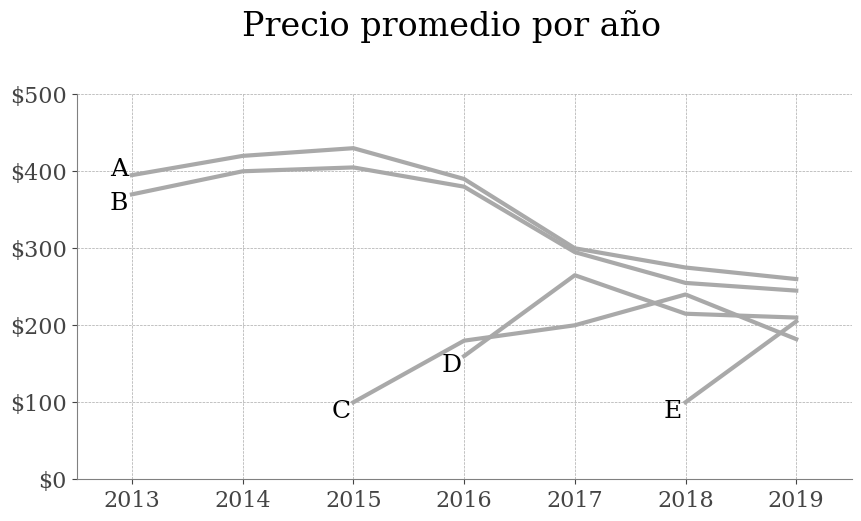
\includegraphics{02_precios_producto_files/figure-pdf/cell-17-output-1.png}

\textbf{Observaciones.} - Para el objetivo planteado, esta gráfica
muestra claramente la tendencia de los precios de los productos A, B, C
, D y E a lo largo del tiempo. - Hemos eliminado información que es
irrelevante para ese objetivo. - Esta visualización se puede usar como
un lienzo para posteriormente resaltar algunas cosas de interés.

\subsection{\texorpdfstring{Enfocar la atención: \emph{preattentive
features}}{Enfocar la atención: preattentive features}}\label{enfocar-la-atenciuxf3n-preattentive-features}

\begin{itemize}
\tightlist
\item
  Finalmente llegamos a un punto interesante: enfocar la atención de la
  audiencia en puntos relevantes mediante el uso estratégico de algunas
  \emph{preattentive features}.
\item
  Consideremos el texto de la visualización inicial:

  \begin{itemize}
  \tightlist
  \item
    \textbf{``Los precios han bajado desde la introducción del producto
    C in 2010.''}
  \item
    Este texto se cambiará por: \textbf{``Después del lanzamiento del
    producto C en 2015, el precio promedio al menudeo de los productos
    existentes ha disminuido.''} Este último es más correcto que el
    primero.
  \end{itemize}
\item
  ¿Cómo se puede demostrar la validez de este último texto usando
  \emph{preattentive features}?
\end{itemize}

\subsubsection{Color y marcadores}\label{color-y-marcadores}

\begin{Shaded}
\begin{Highlighting}[]
\CommentTok{\# Visualización 8: enfocamos la atención en el descenso}
\NormalTok{fig }\OperatorTok{=}\NormalTok{ plt.figure() }\CommentTok{\# Se define una figura}
\NormalTok{ax }\OperatorTok{=}\NormalTok{ fig.gca()     }\CommentTok{\# Se obtienen los ejes de la figura}

\CommentTok{\# Producto A}
\NormalTok{ax.plot(x2, A, lw}\OperatorTok{=}\DecValTok{3}\NormalTok{, c}\OperatorTok{=}\StringTok{\textquotesingle{}darkgray\textquotesingle{}}\NormalTok{)}
\NormalTok{ax.plot(x2[}\DecValTok{2}\NormalTok{:], A[}\DecValTok{2}\NormalTok{:], lw}\OperatorTok{=}\DecValTok{3}\NormalTok{, color}\OperatorTok{=}\StringTok{\textquotesingle{}royalblue\textquotesingle{}}\NormalTok{)}

\CommentTok{\# Producto B}
\NormalTok{ax.plot(x2, B, lw}\OperatorTok{=}\DecValTok{3}\NormalTok{, c}\OperatorTok{=}\StringTok{\textquotesingle{}darkgray\textquotesingle{}}\NormalTok{)}
\NormalTok{plt.plot(x2[}\DecValTok{2}\NormalTok{:], B[}\DecValTok{2}\NormalTok{:], lw}\OperatorTok{=}\DecValTok{3}\NormalTok{, color}\OperatorTok{=}\StringTok{\textquotesingle{}royalblue\textquotesingle{}}\NormalTok{)}

\CommentTok{\# Producto C}
\NormalTok{ax.plot(x2, C, lw}\OperatorTok{=}\DecValTok{3}\NormalTok{, c}\OperatorTok{=}\StringTok{\textquotesingle{}darkgray\textquotesingle{}}\NormalTok{)}
\NormalTok{ax.scatter(x2[}\DecValTok{2}\NormalTok{], C[}\DecValTok{2}\NormalTok{], marker}\OperatorTok{=}\StringTok{\textquotesingle{}o\textquotesingle{}}\NormalTok{, alpha}\OperatorTok{=}\FloatTok{0.85}\NormalTok{, ec }\OperatorTok{=} \StringTok{\textquotesingle{}k\textquotesingle{}}\NormalTok{, s}\OperatorTok{=}\DecValTok{75}\NormalTok{, zorder}\OperatorTok{=}\DecValTok{5}\NormalTok{, color}\OperatorTok{=}\StringTok{\textquotesingle{}royalblue\textquotesingle{}}\NormalTok{)}

\CommentTok{\# Producto D}
\NormalTok{ax.plot(x2, D, lw}\OperatorTok{=}\DecValTok{3}\NormalTok{, c}\OperatorTok{=}\StringTok{\textquotesingle{}darkgray\textquotesingle{}}\NormalTok{)}

\CommentTok{\# Producto E}
\NormalTok{ax.plot(x2, E, lw}\OperatorTok{=}\DecValTok{3}\NormalTok{, c}\OperatorTok{=}\StringTok{\textquotesingle{}darkgray\textquotesingle{}}\NormalTok{)}

\CommentTok{\# Límites en los ejes}
\NormalTok{ax.set\_ylim(}\DecValTok{0}\NormalTok{,}\DecValTok{500}\NormalTok{)}
\NormalTok{ax.set\_xlim(}\FloatTok{2012.5}\NormalTok{,}\FloatTok{2019.5}\NormalTok{)}

\CommentTok{\# Marcas sobre los ejes}
\NormalTok{ax.set\_xticks(ticks}\OperatorTok{=}\NormalTok{[i }\ControlFlowTok{for}\NormalTok{ i }\KeywordTok{in} \BuiltInTok{range}\NormalTok{(}\DecValTok{2013}\NormalTok{,}\DecValTok{2020}\NormalTok{)])}
\NormalTok{ax.set\_yticks(ticks}\OperatorTok{=}\NormalTok{[}\DecValTok{0}\NormalTok{,}\DecValTok{100}\NormalTok{,}\DecValTok{200}\NormalTok{,}\DecValTok{300}\NormalTok{,}\DecValTok{400}\NormalTok{,}\DecValTok{500}\NormalTok{], }
\NormalTok{              labels}\OperatorTok{=}\NormalTok{[}\StringTok{\textquotesingle{}\textbackslash{}$0\textquotesingle{}}\NormalTok{,}\StringTok{\textquotesingle{}\textbackslash{}$100\textquotesingle{}}\NormalTok{,}\StringTok{\textquotesingle{}\textbackslash{}$200\textquotesingle{}}\NormalTok{,}\StringTok{\textquotesingle{}\textbackslash{}$300\textquotesingle{}}\NormalTok{,}\StringTok{\textquotesingle{}\textbackslash{}$400\textquotesingle{}}\NormalTok{,}\StringTok{\textquotesingle{}\textbackslash{}$500\textquotesingle{}}\NormalTok{])}

\CommentTok{\# Rejilla }
\NormalTok{ax.grid()}

\CommentTok{\# Etiquetado de cada línea}
\NormalTok{ax.text(x }\OperatorTok{=}\NormalTok{ x2[}\DecValTok{0}\NormalTok{]}\OperatorTok{{-}}\FloatTok{0.20}\NormalTok{, y }\OperatorTok{=}\NormalTok{ A[}\DecValTok{0}\NormalTok{], s }\OperatorTok{=} \StringTok{\textquotesingle{}A\textquotesingle{}}\NormalTok{, fontsize }\OperatorTok{=} \DecValTok{18}\NormalTok{)}
\NormalTok{ax.text(x }\OperatorTok{=}\NormalTok{ x2[}\DecValTok{0}\NormalTok{]}\OperatorTok{{-}}\FloatTok{0.20}\NormalTok{, y }\OperatorTok{=}\NormalTok{ B[}\DecValTok{0}\NormalTok{]}\OperatorTok{{-}}\DecValTok{20}\NormalTok{, s }\OperatorTok{=} \StringTok{\textquotesingle{}B\textquotesingle{}}\NormalTok{, fontsize }\OperatorTok{=} \DecValTok{18}\NormalTok{)}
\NormalTok{ax.text(x }\OperatorTok{=}\NormalTok{ x2[}\DecValTok{2}\NormalTok{]}\OperatorTok{{-}}\FloatTok{0.20}\NormalTok{, y }\OperatorTok{=}\NormalTok{ C[}\DecValTok{2}\NormalTok{]}\OperatorTok{{-}}\DecValTok{20}\NormalTok{, s }\OperatorTok{=} \StringTok{\textquotesingle{}C\textquotesingle{}}\NormalTok{, fontsize }\OperatorTok{=} \DecValTok{18}\NormalTok{)}
\NormalTok{ax.text(x }\OperatorTok{=}\NormalTok{ x2[}\DecValTok{3}\NormalTok{]}\OperatorTok{{-}}\FloatTok{0.20}\NormalTok{, y }\OperatorTok{=}\NormalTok{ D[}\DecValTok{3}\NormalTok{]}\OperatorTok{{-}}\DecValTok{20}\NormalTok{, s }\OperatorTok{=} \StringTok{\textquotesingle{}D\textquotesingle{}}\NormalTok{, fontsize }\OperatorTok{=} \DecValTok{18}\NormalTok{)}
\NormalTok{ax.text(x }\OperatorTok{=}\NormalTok{ x2[}\DecValTok{5}\NormalTok{]}\OperatorTok{{-}}\FloatTok{0.20}\NormalTok{, y }\OperatorTok{=}\NormalTok{ E[}\DecValTok{5}\NormalTok{]}\OperatorTok{{-}}\DecValTok{20}\NormalTok{, s }\OperatorTok{=} \StringTok{\textquotesingle{}E\textquotesingle{}}\NormalTok{, fontsize }\OperatorTok{=} \DecValTok{18}\NormalTok{)}

\CommentTok{\# Eliminación de algunas líneas del recuadro}
\NormalTok{ax.spines[}\StringTok{\textquotesingle{}right\textquotesingle{}}\NormalTok{].set\_visible(}\VariableTok{False}\NormalTok{)}
\NormalTok{ax.spines[}\StringTok{\textquotesingle{}top\textquotesingle{}}\NormalTok{].set\_visible(}\VariableTok{False}\NormalTok{)}
\NormalTok{ax.spines[}\StringTok{\textquotesingle{}left\textquotesingle{}}\NormalTok{].set\_color(}\StringTok{\textquotesingle{}gray\textquotesingle{}}\NormalTok{)}
\NormalTok{ax.spines[}\StringTok{\textquotesingle{}bottom\textquotesingle{}}\NormalTok{].set\_color(}\StringTok{\textquotesingle{}gray\textquotesingle{}}\NormalTok{)}

\CommentTok{\# Color de los ticks}
\NormalTok{ax.tick\_params(axis}\OperatorTok{=}\StringTok{\textquotesingle{}x\textquotesingle{}}\NormalTok{, colors}\OperatorTok{=}\StringTok{\textquotesingle{}\#444444\textquotesingle{}}\NormalTok{)}
\NormalTok{ax.tick\_params(axis}\OperatorTok{=}\StringTok{\textquotesingle{}y\textquotesingle{}}\NormalTok{, colors}\OperatorTok{=}\StringTok{\textquotesingle{}\#444444\textquotesingle{}}\NormalTok{)}

\NormalTok{plt.suptitle(}\StringTok{\textquotesingle{}Precio promedio por año\textquotesingle{}}\NormalTok{, fontsize}\OperatorTok{=}\DecValTok{24}\NormalTok{, y}\OperatorTok{=}\FloatTok{1.05}\NormalTok{)}
\NormalTok{plt.show()}
\end{Highlighting}
\end{Shaded}

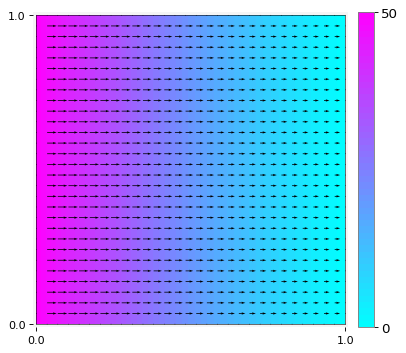
\includegraphics{02_precios_producto_files/figure-pdf/cell-18-output-1.png}

\textbf{Observaciones.}

\begin{itemize}
\tightlist
\item
  En esta última visualización estamos enfocando la atención del público
  usando un color sobre las gráficas de los productos A y B: se resalta
  el descenso del precio.
\item
  Adicionalmente, se agrega un marcador con el mismo color en el inicio
  de la curva del producto C, para indicar cuando se introdujo.
\item
  Se ve claramente el inicio de C y qué pasó con A y B posterior a eso.
\item
  Se usa el color de manera consistente.
\end{itemize}

\subsubsection{Subida y bajada del
precio}\label{subida-y-bajada-del-precio}

\begin{Shaded}
\begin{Highlighting}[]
\CommentTok{\# Visualización 9: enfocamos la atención en el ascenso y descenso}
\NormalTok{fig }\OperatorTok{=}\NormalTok{ plt.figure() }\CommentTok{\# Se define una figura}
\NormalTok{ax }\OperatorTok{=}\NormalTok{ fig.gca()     }\CommentTok{\# Se obtienen los ejes de la figura}

\CommentTok{\# Producto A}
\NormalTok{ax.plot(x2[}\DecValTok{2}\NormalTok{:], A[}\DecValTok{2}\NormalTok{:], lw}\OperatorTok{=}\DecValTok{3}\NormalTok{, color}\OperatorTok{=}\StringTok{\textquotesingle{}royalblue\textquotesingle{}}\NormalTok{)}
\NormalTok{ax.plot(x2[}\DecValTok{0}\NormalTok{:}\DecValTok{3}\NormalTok{], A[}\DecValTok{0}\NormalTok{:}\DecValTok{3}\NormalTok{], lw}\OperatorTok{=}\DecValTok{3}\NormalTok{, color}\OperatorTok{=}\StringTok{\textquotesingle{}firebrick\textquotesingle{}}\NormalTok{)}

\CommentTok{\# Producto B}
\NormalTok{ax.plot(x2[}\DecValTok{2}\NormalTok{:], B[}\DecValTok{2}\NormalTok{:], lw}\OperatorTok{=}\DecValTok{3}\NormalTok{, color}\OperatorTok{=}\StringTok{\textquotesingle{}royalblue\textquotesingle{}}\NormalTok{)}
\NormalTok{ax.plot(x2[}\DecValTok{0}\NormalTok{:}\DecValTok{3}\NormalTok{], B[}\DecValTok{0}\NormalTok{:}\DecValTok{3}\NormalTok{], lw}\OperatorTok{=}\DecValTok{3}\NormalTok{, color}\OperatorTok{=}\StringTok{\textquotesingle{}firebrick\textquotesingle{}}\NormalTok{)}

\CommentTok{\# Producto C}
\NormalTok{ax.plot(x2[}\DecValTok{5}\NormalTok{:], C[}\DecValTok{5}\NormalTok{:], lw}\OperatorTok{=}\DecValTok{3}\NormalTok{, color}\OperatorTok{=}\StringTok{\textquotesingle{}royalblue\textquotesingle{}}\NormalTok{)}
\NormalTok{ax.plot(x2[}\DecValTok{2}\NormalTok{:}\DecValTok{6}\NormalTok{], C[}\DecValTok{2}\NormalTok{:}\DecValTok{6}\NormalTok{], lw}\OperatorTok{=}\DecValTok{3}\NormalTok{, color}\OperatorTok{=}\StringTok{\textquotesingle{}firebrick\textquotesingle{}}\NormalTok{)}

\CommentTok{\# Producto D}
\NormalTok{ax.plot(x2[}\DecValTok{4}\NormalTok{:], D[}\DecValTok{4}\NormalTok{:], lw}\OperatorTok{=}\DecValTok{3}\NormalTok{, color}\OperatorTok{=}\StringTok{\textquotesingle{}royalblue\textquotesingle{}}\NormalTok{)}
\NormalTok{ax.plot(x2[}\DecValTok{3}\NormalTok{:}\DecValTok{5}\NormalTok{], D[}\DecValTok{3}\NormalTok{:}\DecValTok{5}\NormalTok{], lw}\OperatorTok{=}\DecValTok{3}\NormalTok{, color}\OperatorTok{=}\StringTok{\textquotesingle{}firebrick\textquotesingle{}}\NormalTok{)}

\CommentTok{\# Producto E}
\NormalTok{ax.plot(x2, E, lw}\OperatorTok{=}\DecValTok{3}\NormalTok{, c}\OperatorTok{=}\StringTok{\textquotesingle{}firebrick\textquotesingle{}}\NormalTok{)}

\CommentTok{\# Límites en los ejes}
\NormalTok{ax.set\_ylim(}\DecValTok{0}\NormalTok{,}\DecValTok{500}\NormalTok{)}
\NormalTok{ax.set\_xlim(}\FloatTok{2012.5}\NormalTok{,}\FloatTok{2019.5}\NormalTok{)}

\CommentTok{\# Marcas sobre los ejes}
\NormalTok{ax.set\_xticks(ticks}\OperatorTok{=}\NormalTok{[i }\ControlFlowTok{for}\NormalTok{ i }\KeywordTok{in} \BuiltInTok{range}\NormalTok{(}\DecValTok{2013}\NormalTok{,}\DecValTok{2020}\NormalTok{)])}
\NormalTok{ax.set\_yticks(ticks}\OperatorTok{=}\NormalTok{[}\DecValTok{0}\NormalTok{,}\DecValTok{100}\NormalTok{,}\DecValTok{200}\NormalTok{,}\DecValTok{300}\NormalTok{,}\DecValTok{400}\NormalTok{,}\DecValTok{500}\NormalTok{], }
\NormalTok{              labels}\OperatorTok{=}\NormalTok{[}\StringTok{\textquotesingle{}\textbackslash{}$0\textquotesingle{}}\NormalTok{,}\StringTok{\textquotesingle{}\textbackslash{}$100\textquotesingle{}}\NormalTok{,}\StringTok{\textquotesingle{}\textbackslash{}$200\textquotesingle{}}\NormalTok{,}\StringTok{\textquotesingle{}\textbackslash{}$300\textquotesingle{}}\NormalTok{,}\StringTok{\textquotesingle{}\textbackslash{}$400\textquotesingle{}}\NormalTok{,}\StringTok{\textquotesingle{}\textbackslash{}$500\textquotesingle{}}\NormalTok{])}

\CommentTok{\# Rejilla}
\NormalTok{ax.grid()}

\CommentTok{\# Etiquetado de cada línea}
\NormalTok{ax.text(x }\OperatorTok{=}\NormalTok{ x2[}\DecValTok{0}\NormalTok{]}\OperatorTok{{-}}\FloatTok{0.20}\NormalTok{, y }\OperatorTok{=}\NormalTok{ A[}\DecValTok{0}\NormalTok{], s }\OperatorTok{=} \StringTok{\textquotesingle{}A\textquotesingle{}}\NormalTok{, fontsize }\OperatorTok{=} \DecValTok{18}\NormalTok{)}
\NormalTok{ax.text(x }\OperatorTok{=}\NormalTok{ x2[}\DecValTok{0}\NormalTok{]}\OperatorTok{{-}}\FloatTok{0.20}\NormalTok{, y }\OperatorTok{=}\NormalTok{ B[}\DecValTok{0}\NormalTok{]}\OperatorTok{{-}}\DecValTok{20}\NormalTok{, s }\OperatorTok{=} \StringTok{\textquotesingle{}B\textquotesingle{}}\NormalTok{, fontsize }\OperatorTok{=} \DecValTok{18}\NormalTok{)}
\NormalTok{ax.text(x }\OperatorTok{=}\NormalTok{ x2[}\DecValTok{2}\NormalTok{]}\OperatorTok{{-}}\FloatTok{0.20}\NormalTok{, y }\OperatorTok{=}\NormalTok{ C[}\DecValTok{2}\NormalTok{]}\OperatorTok{{-}}\DecValTok{20}\NormalTok{, s }\OperatorTok{=} \StringTok{\textquotesingle{}C\textquotesingle{}}\NormalTok{, fontsize }\OperatorTok{=} \DecValTok{18}\NormalTok{)}
\NormalTok{ax.text(x }\OperatorTok{=}\NormalTok{ x2[}\DecValTok{3}\NormalTok{]}\OperatorTok{{-}}\FloatTok{0.20}\NormalTok{, y }\OperatorTok{=}\NormalTok{ D[}\DecValTok{3}\NormalTok{]}\OperatorTok{{-}}\DecValTok{20}\NormalTok{, s }\OperatorTok{=} \StringTok{\textquotesingle{}D\textquotesingle{}}\NormalTok{, fontsize }\OperatorTok{=} \DecValTok{18}\NormalTok{)}
\NormalTok{ax.text(x }\OperatorTok{=}\NormalTok{ x2[}\DecValTok{5}\NormalTok{]}\OperatorTok{{-}}\FloatTok{0.20}\NormalTok{, y }\OperatorTok{=}\NormalTok{ E[}\DecValTok{5}\NormalTok{]}\OperatorTok{{-}}\DecValTok{20}\NormalTok{, s }\OperatorTok{=} \StringTok{\textquotesingle{}E\textquotesingle{}}\NormalTok{, fontsize }\OperatorTok{=} \DecValTok{18}\NormalTok{)}

\CommentTok{\# Eliminación de algunas líneas del recuadro}
\NormalTok{ax.spines[}\StringTok{\textquotesingle{}right\textquotesingle{}}\NormalTok{].set\_visible(}\VariableTok{False}\NormalTok{)}
\NormalTok{ax.spines[}\StringTok{\textquotesingle{}top\textquotesingle{}}\NormalTok{].set\_visible(}\VariableTok{False}\NormalTok{)}
\NormalTok{ax.spines[}\StringTok{\textquotesingle{}left\textquotesingle{}}\NormalTok{].set\_color(}\StringTok{\textquotesingle{}gray\textquotesingle{}}\NormalTok{)}
\NormalTok{ax.spines[}\StringTok{\textquotesingle{}bottom\textquotesingle{}}\NormalTok{].set\_color(}\StringTok{\textquotesingle{}gray\textquotesingle{}}\NormalTok{)}

\CommentTok{\# Color de los ticks}
\NormalTok{ax.tick\_params(axis}\OperatorTok{=}\StringTok{\textquotesingle{}x\textquotesingle{}}\NormalTok{, colors}\OperatorTok{=}\StringTok{\textquotesingle{}\#444444\textquotesingle{}}\NormalTok{)}
\NormalTok{ax.tick\_params(axis}\OperatorTok{=}\StringTok{\textquotesingle{}y\textquotesingle{}}\NormalTok{, colors}\OperatorTok{=}\StringTok{\textquotesingle{}\#444444\textquotesingle{}}\NormalTok{)}

\NormalTok{plt.suptitle(}\StringTok{\textquotesingle{}Precio promedio por año\textquotesingle{}}\NormalTok{, fontsize}\OperatorTok{=}\DecValTok{24}\NormalTok{, y}\OperatorTok{=}\FloatTok{1.05}\NormalTok{)}
\NormalTok{plt.show()}
\end{Highlighting}
\end{Shaded}

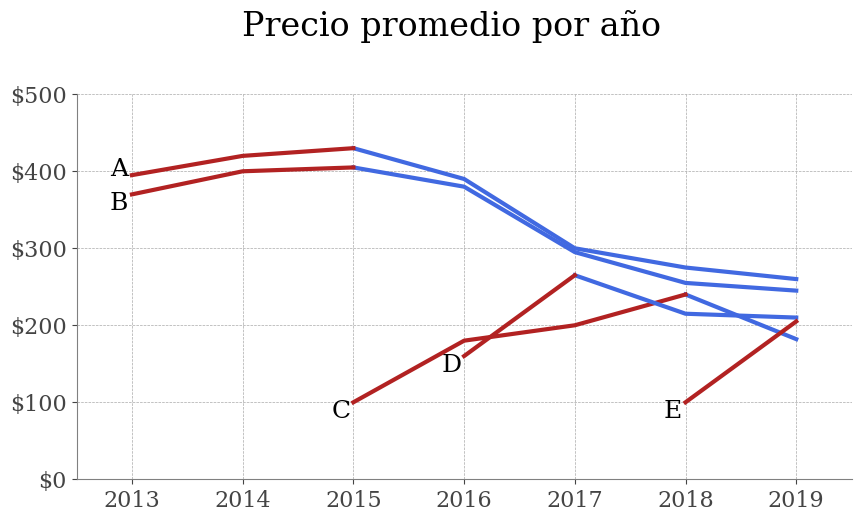
\includegraphics{02_precios_producto_files/figure-pdf/cell-19-output-1.png}

\textbf{Observaciones.}

En esta gráfica se muestra que usando la misma estrategia, se puede
resaltar el hecho de que: con el lanzamiento de un nuevo producto, es
típico ver un ascenso inicial (parte roja) del precio promedio al
menudeo, seguido de un descenso (parte azul).

\subsubsection{Precio final}\label{precio-final}

\begin{Shaded}
\begin{Highlighting}[]
\CommentTok{\# Visualización 10: marcamos los precios finales}
\NormalTok{fig }\OperatorTok{=}\NormalTok{ plt.figure() }\CommentTok{\# Se define una figura}
\NormalTok{ax }\OperatorTok{=}\NormalTok{ fig.gca()     }\CommentTok{\# Se obtienen los ejes de la figura}

\CommentTok{\# Producto A}
\NormalTok{ax.plot(x2, A, lw}\OperatorTok{=}\DecValTok{3}\NormalTok{, c}\OperatorTok{=}\StringTok{\textquotesingle{}darkgray\textquotesingle{}}\NormalTok{)}
\NormalTok{ax.scatter(x2[}\OperatorTok{{-}}\DecValTok{1}\NormalTok{], A[}\OperatorTok{{-}}\DecValTok{1}\NormalTok{], marker}\OperatorTok{=}\StringTok{\textquotesingle{}o\textquotesingle{}}\NormalTok{, alpha}\OperatorTok{=}\FloatTok{0.85}\NormalTok{, ec }\OperatorTok{=} \StringTok{\textquotesingle{}k\textquotesingle{}}\NormalTok{, s}\OperatorTok{=}\DecValTok{75}\NormalTok{, zorder}\OperatorTok{=}\DecValTok{5}\NormalTok{, color}\OperatorTok{=}\StringTok{\textquotesingle{}royalblue\textquotesingle{}}\NormalTok{)}

\CommentTok{\# Producto B}
\NormalTok{ax.plot(x2, B, lw}\OperatorTok{=}\DecValTok{3}\NormalTok{, c}\OperatorTok{=}\StringTok{\textquotesingle{}darkgray\textquotesingle{}}\NormalTok{)}
\NormalTok{ax.scatter(x2[}\OperatorTok{{-}}\DecValTok{1}\NormalTok{], B[}\OperatorTok{{-}}\DecValTok{1}\NormalTok{], marker}\OperatorTok{=}\StringTok{\textquotesingle{}o\textquotesingle{}}\NormalTok{, alpha}\OperatorTok{=}\FloatTok{0.85}\NormalTok{, ec }\OperatorTok{=} \StringTok{\textquotesingle{}k\textquotesingle{}}\NormalTok{, s}\OperatorTok{=}\DecValTok{75}\NormalTok{, zorder}\OperatorTok{=}\DecValTok{5}\NormalTok{, color}\OperatorTok{=}\StringTok{\textquotesingle{}royalblue\textquotesingle{}}\NormalTok{)}

\CommentTok{\# Producto C}
\NormalTok{ax.plot(x2, C, lw}\OperatorTok{=}\DecValTok{3}\NormalTok{, c}\OperatorTok{=}\StringTok{\textquotesingle{}darkgray\textquotesingle{}}\NormalTok{)}
\NormalTok{ax.scatter(x2[}\OperatorTok{{-}}\DecValTok{1}\NormalTok{], C[}\OperatorTok{{-}}\DecValTok{1}\NormalTok{], marker}\OperatorTok{=}\StringTok{\textquotesingle{}o\textquotesingle{}}\NormalTok{, alpha}\OperatorTok{=}\FloatTok{0.85}\NormalTok{, ec }\OperatorTok{=} \StringTok{\textquotesingle{}k\textquotesingle{}}\NormalTok{, s}\OperatorTok{=}\DecValTok{75}\NormalTok{, zorder}\OperatorTok{=}\DecValTok{5}\NormalTok{, color}\OperatorTok{=}\StringTok{\textquotesingle{}royalblue\textquotesingle{}}\NormalTok{)}

\CommentTok{\# Producto D}
\NormalTok{ax.plot(x2, D, lw}\OperatorTok{=}\DecValTok{3}\NormalTok{, c}\OperatorTok{=}\StringTok{\textquotesingle{}darkgray\textquotesingle{}}\NormalTok{)}
\NormalTok{ax.scatter(x2[}\OperatorTok{{-}}\DecValTok{1}\NormalTok{], D[}\OperatorTok{{-}}\DecValTok{1}\NormalTok{], marker}\OperatorTok{=}\StringTok{\textquotesingle{}o\textquotesingle{}}\NormalTok{, alpha}\OperatorTok{=}\FloatTok{0.85}\NormalTok{, ec }\OperatorTok{=} \StringTok{\textquotesingle{}k\textquotesingle{}}\NormalTok{, s}\OperatorTok{=}\DecValTok{75}\NormalTok{, zorder}\OperatorTok{=}\DecValTok{5}\NormalTok{, color}\OperatorTok{=}\StringTok{\textquotesingle{}royalblue\textquotesingle{}}\NormalTok{)}

\CommentTok{\# Producto E}
\NormalTok{ax.plot(x2, E, lw}\OperatorTok{=}\DecValTok{3}\NormalTok{, c}\OperatorTok{=}\StringTok{\textquotesingle{}silver\textquotesingle{}}\NormalTok{)}
\NormalTok{ax.scatter(x2[}\OperatorTok{{-}}\DecValTok{1}\NormalTok{], E[}\OperatorTok{{-}}\DecValTok{1}\NormalTok{], marker}\OperatorTok{=}\StringTok{\textquotesingle{}o\textquotesingle{}}\NormalTok{, alpha}\OperatorTok{=}\FloatTok{0.85}\NormalTok{, ec }\OperatorTok{=} \StringTok{\textquotesingle{}k\textquotesingle{}}\NormalTok{, s}\OperatorTok{=}\DecValTok{75}\NormalTok{, zorder}\OperatorTok{=}\DecValTok{5}\NormalTok{, color}\OperatorTok{=}\StringTok{\textquotesingle{}royalblue\textquotesingle{}}\NormalTok{)}

\CommentTok{\# Límites en los ejes}
\NormalTok{ax.set\_ylim(}\DecValTok{0}\NormalTok{,}\DecValTok{500}\NormalTok{)}
\NormalTok{ax.set\_xlim(}\FloatTok{2012.5}\NormalTok{,}\FloatTok{2019.5}\NormalTok{)}

\CommentTok{\# Marcas sobre los ejes}
\NormalTok{ax.set\_xticks(ticks}\OperatorTok{=}\NormalTok{[i }\ControlFlowTok{for}\NormalTok{ i }\KeywordTok{in} \BuiltInTok{range}\NormalTok{(}\DecValTok{2013}\NormalTok{,}\DecValTok{2020}\NormalTok{)])}
\NormalTok{ax.set\_yticks(ticks}\OperatorTok{=}\NormalTok{[}\DecValTok{0}\NormalTok{,}\DecValTok{100}\NormalTok{,}\DecValTok{200}\NormalTok{,}\DecValTok{300}\NormalTok{,}\DecValTok{400}\NormalTok{,}\DecValTok{500}\NormalTok{], }
\NormalTok{              labels}\OperatorTok{=}\NormalTok{[}\StringTok{\textquotesingle{}\textbackslash{}$0\textquotesingle{}}\NormalTok{,}\StringTok{\textquotesingle{}\textbackslash{}$100\textquotesingle{}}\NormalTok{,}\StringTok{\textquotesingle{}\textbackslash{}$200\textquotesingle{}}\NormalTok{,}\StringTok{\textquotesingle{}\textbackslash{}$300\textquotesingle{}}\NormalTok{,}\StringTok{\textquotesingle{}\textbackslash{}$400\textquotesingle{}}\NormalTok{,}\StringTok{\textquotesingle{}\textbackslash{}$500\textquotesingle{}}\NormalTok{])}

\CommentTok{\# Rejilla}
\NormalTok{ax.grid()}

\CommentTok{\# Etiquetado de cada línea}
\NormalTok{ax.text(x }\OperatorTok{=}\NormalTok{ x2[}\DecValTok{0}\NormalTok{]}\OperatorTok{{-}}\FloatTok{0.20}\NormalTok{, y }\OperatorTok{=}\NormalTok{ A[}\DecValTok{0}\NormalTok{], s }\OperatorTok{=} \StringTok{\textquotesingle{}A\textquotesingle{}}\NormalTok{, fontsize }\OperatorTok{=} \DecValTok{18}\NormalTok{)}
\NormalTok{ax.text(x }\OperatorTok{=}\NormalTok{ x2[}\DecValTok{0}\NormalTok{]}\OperatorTok{{-}}\FloatTok{0.20}\NormalTok{, y }\OperatorTok{=}\NormalTok{ B[}\DecValTok{0}\NormalTok{]}\OperatorTok{{-}}\DecValTok{20}\NormalTok{, s }\OperatorTok{=} \StringTok{\textquotesingle{}B\textquotesingle{}}\NormalTok{, fontsize }\OperatorTok{=} \DecValTok{18}\NormalTok{)}
\NormalTok{ax.text(x }\OperatorTok{=}\NormalTok{ x2[}\DecValTok{2}\NormalTok{]}\OperatorTok{{-}}\FloatTok{0.20}\NormalTok{, y }\OperatorTok{=}\NormalTok{ C[}\DecValTok{2}\NormalTok{]}\OperatorTok{{-}}\DecValTok{20}\NormalTok{, s }\OperatorTok{=} \StringTok{\textquotesingle{}C\textquotesingle{}}\NormalTok{, fontsize }\OperatorTok{=} \DecValTok{18}\NormalTok{)}
\NormalTok{ax.text(x }\OperatorTok{=}\NormalTok{ x2[}\DecValTok{3}\NormalTok{]}\OperatorTok{{-}}\FloatTok{0.20}\NormalTok{, y }\OperatorTok{=}\NormalTok{ D[}\DecValTok{3}\NormalTok{]}\OperatorTok{{-}}\DecValTok{20}\NormalTok{, s }\OperatorTok{=} \StringTok{\textquotesingle{}D\textquotesingle{}}\NormalTok{, fontsize }\OperatorTok{=} \DecValTok{18}\NormalTok{)}
\NormalTok{ax.text(x }\OperatorTok{=}\NormalTok{ x2[}\DecValTok{5}\NormalTok{]}\OperatorTok{{-}}\FloatTok{0.20}\NormalTok{, y }\OperatorTok{=}\NormalTok{ E[}\DecValTok{5}\NormalTok{]}\OperatorTok{{-}}\DecValTok{20}\NormalTok{, s }\OperatorTok{=} \StringTok{\textquotesingle{}E\textquotesingle{}}\NormalTok{, fontsize }\OperatorTok{=} \DecValTok{18}\NormalTok{)}

\CommentTok{\# Eliminación de algunas líneas del recuadro}
\NormalTok{ax.spines[}\StringTok{\textquotesingle{}right\textquotesingle{}}\NormalTok{].set\_visible(}\VariableTok{False}\NormalTok{)}
\NormalTok{ax.spines[}\StringTok{\textquotesingle{}top\textquotesingle{}}\NormalTok{].set\_visible(}\VariableTok{False}\NormalTok{)}
\NormalTok{ax.spines[}\StringTok{\textquotesingle{}left\textquotesingle{}}\NormalTok{].set\_color(}\StringTok{\textquotesingle{}gray\textquotesingle{}}\NormalTok{)}
\NormalTok{ax.spines[}\StringTok{\textquotesingle{}bottom\textquotesingle{}}\NormalTok{].set\_color(}\StringTok{\textquotesingle{}gray\textquotesingle{}}\NormalTok{)}

\CommentTok{\# Color de los ticks}
\NormalTok{ax.tick\_params(axis}\OperatorTok{=}\StringTok{\textquotesingle{}x\textquotesingle{}}\NormalTok{, colors}\OperatorTok{=}\StringTok{\textquotesingle{}\#444444\textquotesingle{}}\NormalTok{)}
\NormalTok{ax.tick\_params(axis}\OperatorTok{=}\StringTok{\textquotesingle{}y\textquotesingle{}}\NormalTok{, colors}\OperatorTok{=}\StringTok{\textquotesingle{}\#444444\textquotesingle{}}\NormalTok{)}

\NormalTok{plt.suptitle(}\StringTok{\textquotesingle{}Precio promedio por año\textquotesingle{}}\NormalTok{, fontsize}\OperatorTok{=}\DecValTok{24}\NormalTok{, y}\OperatorTok{=}\FloatTok{1.05}\NormalTok{)}
\NormalTok{plt.show()}
\end{Highlighting}
\end{Shaded}

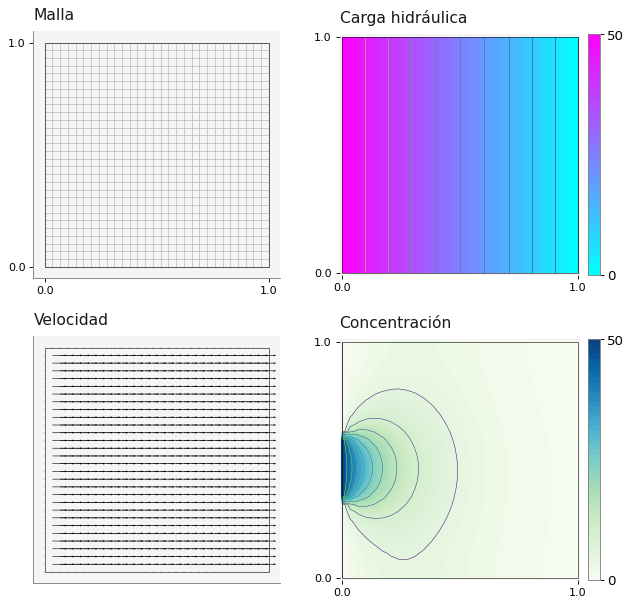
\includegraphics{02_precios_producto_files/figure-pdf/cell-20-output-1.png}

\textbf{Observación}

\begin{itemize}
\tightlist
\item
  En esta gráfica se muestra que: en 2019, los precios de todos los
  productos al menudeo convergen al intervalo de \([180, 260]\) con un
  promedio de \(220\).
\item
  Quizá sea necesario agregar estos números en el gráfico para mayor
  claridad.
\item
  Se usan marcadores y colores para llevar nuestra atención hacia los
  precios finales.
\end{itemize}

\subsection{Pensar como diseñador}\label{pensar-como-diseuxf1ador}

\begin{itemize}
\tightlist
\item
  Durante todo el proceso hemos estado pensando como diseñadores,
  pensando en los colores, las líneas, los marcadores y toda la
  decoración de la gráfica, y cómo resaltar lo que es importante.
\item
  Se puede hacer un poco más:

  \begin{itemize}
  \tightlist
  \item
    Agregar textos simples a los ejes. Se debe tener cuidado con el uso
    de mayúsculas, solo poner mayúscula la primera letra de un título.
  \item
    Alinear cada elemento, en este caso, los títulos.
  \end{itemize}
\item
  Además, vamos a agregar una región donde se recomienda debe estar el
  precio de lanzamiento de nuestro producto.
\end{itemize}

\begin{Shaded}
\begin{Highlighting}[]
\CommentTok{\# Visualización 11: marcamos el rango de precios de introducción}
\NormalTok{fig }\OperatorTok{=}\NormalTok{ plt.figure() }\CommentTok{\# Se define una figura}
\NormalTok{ax }\OperatorTok{=}\NormalTok{ fig.gca()     }\CommentTok{\# Se obtienen los ejes de la figura}

\CommentTok{\# Producto A}
\NormalTok{ax.plot(x2, A, lw}\OperatorTok{=}\DecValTok{3}\NormalTok{, c}\OperatorTok{=}\StringTok{\textquotesingle{}darkgray\textquotesingle{}}\NormalTok{)}
\NormalTok{ax.scatter(x2[}\OperatorTok{{-}}\DecValTok{1}\NormalTok{], A[}\OperatorTok{{-}}\DecValTok{1}\NormalTok{], marker}\OperatorTok{=}\StringTok{\textquotesingle{}o\textquotesingle{}}\NormalTok{, alpha}\OperatorTok{=}\FloatTok{0.85}\NormalTok{, ec }\OperatorTok{=} \StringTok{\textquotesingle{}k\textquotesingle{}}\NormalTok{, s}\OperatorTok{=}\DecValTok{75}\NormalTok{, zorder}\OperatorTok{=}\DecValTok{5}\NormalTok{, color}\OperatorTok{=}\StringTok{\textquotesingle{}forestgreen\textquotesingle{}}\NormalTok{)}

\CommentTok{\# Producto B}
\NormalTok{ax.plot(x2, B, lw}\OperatorTok{=}\DecValTok{3}\NormalTok{, c}\OperatorTok{=}\StringTok{\textquotesingle{}darkgray\textquotesingle{}}\NormalTok{)}
\NormalTok{ax.scatter(x2[}\OperatorTok{{-}}\DecValTok{1}\NormalTok{], B[}\OperatorTok{{-}}\DecValTok{1}\NormalTok{], marker}\OperatorTok{=}\StringTok{\textquotesingle{}o\textquotesingle{}}\NormalTok{, alpha}\OperatorTok{=}\FloatTok{0.85}\NormalTok{, ec }\OperatorTok{=} \StringTok{\textquotesingle{}k\textquotesingle{}}\NormalTok{, s}\OperatorTok{=}\DecValTok{75}\NormalTok{, zorder}\OperatorTok{=}\DecValTok{5}\NormalTok{, color}\OperatorTok{=}\StringTok{\textquotesingle{}forestgreen\textquotesingle{}}\NormalTok{)}

\CommentTok{\# Producto C}
\NormalTok{ax.plot(x2, C, lw}\OperatorTok{=}\DecValTok{3}\NormalTok{, c}\OperatorTok{=}\StringTok{\textquotesingle{}darkgray\textquotesingle{}}\NormalTok{)}
\NormalTok{ax.scatter(x2[}\OperatorTok{{-}}\DecValTok{1}\NormalTok{], C[}\OperatorTok{{-}}\DecValTok{1}\NormalTok{], marker}\OperatorTok{=}\StringTok{\textquotesingle{}o\textquotesingle{}}\NormalTok{, alpha}\OperatorTok{=}\FloatTok{0.85}\NormalTok{, ec }\OperatorTok{=} \StringTok{\textquotesingle{}k\textquotesingle{}}\NormalTok{, s}\OperatorTok{=}\DecValTok{75}\NormalTok{, zorder}\OperatorTok{=}\DecValTok{5}\NormalTok{, color}\OperatorTok{=}\StringTok{\textquotesingle{}forestgreen\textquotesingle{}}\NormalTok{)}

\CommentTok{\# Producto D}
\NormalTok{ax.plot(x2, D, lw}\OperatorTok{=}\DecValTok{3}\NormalTok{, c}\OperatorTok{=}\StringTok{\textquotesingle{}darkgray\textquotesingle{}}\NormalTok{)}
\NormalTok{ax.scatter(x2[}\OperatorTok{{-}}\DecValTok{1}\NormalTok{], D[}\OperatorTok{{-}}\DecValTok{1}\NormalTok{], marker}\OperatorTok{=}\StringTok{\textquotesingle{}o\textquotesingle{}}\NormalTok{, alpha}\OperatorTok{=}\FloatTok{0.85}\NormalTok{, ec }\OperatorTok{=} \StringTok{\textquotesingle{}k\textquotesingle{}}\NormalTok{, s}\OperatorTok{=}\DecValTok{75}\NormalTok{, zorder}\OperatorTok{=}\DecValTok{5}\NormalTok{, color}\OperatorTok{=}\StringTok{\textquotesingle{}forestgreen\textquotesingle{}}\NormalTok{)}

\CommentTok{\# Producto E}
\NormalTok{ax.plot(x2, E, lw}\OperatorTok{=}\DecValTok{3}\NormalTok{, c}\OperatorTok{=}\StringTok{\textquotesingle{}darkgray\textquotesingle{}}\NormalTok{)}
\NormalTok{ax.scatter(x2[}\OperatorTok{{-}}\DecValTok{1}\NormalTok{], E[}\OperatorTok{{-}}\DecValTok{1}\NormalTok{], marker}\OperatorTok{=}\StringTok{\textquotesingle{}o\textquotesingle{}}\NormalTok{, alpha}\OperatorTok{=}\FloatTok{0.85}\NormalTok{, ec }\OperatorTok{=} \StringTok{\textquotesingle{}k\textquotesingle{}}\NormalTok{, s}\OperatorTok{=}\DecValTok{75}\NormalTok{, zorder}\OperatorTok{=}\DecValTok{5}\NormalTok{, color}\OperatorTok{=}\StringTok{\textquotesingle{}forestgreen\textquotesingle{}}\NormalTok{)}

\CommentTok{\# Promedio final}
\NormalTok{precios\_finales }\OperatorTok{=}\NormalTok{ np.array([A[}\OperatorTok{{-}}\DecValTok{1}\NormalTok{], B[}\OperatorTok{{-}}\DecValTok{1}\NormalTok{], C[}\OperatorTok{{-}}\DecValTok{1}\NormalTok{], D[}\OperatorTok{{-}}\DecValTok{1}\NormalTok{], E[}\OperatorTok{{-}}\DecValTok{1}\NormalTok{],])}
\NormalTok{promedio\_final }\OperatorTok{=}\NormalTok{ np.mean(precios\_finales)}
\NormalTok{ax.scatter(x2[}\OperatorTok{{-}}\DecValTok{1}\NormalTok{], promedio\_final, marker}\OperatorTok{=}\StringTok{\textquotesingle{}\textless{}\textquotesingle{}}\NormalTok{, alpha}\OperatorTok{=}\FloatTok{0.85}\NormalTok{, ec }\OperatorTok{=} \StringTok{\textquotesingle{}k\textquotesingle{}}\NormalTok{, s}\OperatorTok{=}\DecValTok{75}\NormalTok{, }
\NormalTok{           zorder}\OperatorTok{=}\DecValTok{5}\NormalTok{, color}\OperatorTok{=}\StringTok{\textquotesingle{}orange\textquotesingle{}}\NormalTok{, label}\OperatorTok{=}\StringTok{\textquotesingle{}Promedio\textquotesingle{}}\NormalTok{)}

\CommentTok{\# Límites en los ejes}
\NormalTok{ax.set\_ylim(}\DecValTok{0}\NormalTok{,}\DecValTok{500}\NormalTok{)}
\NormalTok{ax.set\_xlim(}\FloatTok{2012.5}\NormalTok{,}\FloatTok{2019.5}\NormalTok{)}

\CommentTok{\# Marcas sobre los ejes}
\NormalTok{ax.set\_xticks(ticks}\OperatorTok{=}\NormalTok{[i }\ControlFlowTok{for}\NormalTok{ i }\KeywordTok{in} \BuiltInTok{range}\NormalTok{(}\DecValTok{2013}\NormalTok{,}\DecValTok{2020}\NormalTok{)])}
\NormalTok{ax.set\_yticks(ticks}\OperatorTok{=}\NormalTok{[}\DecValTok{0}\NormalTok{,}\DecValTok{100}\NormalTok{,}\DecValTok{200}\NormalTok{,}\DecValTok{300}\NormalTok{,}\DecValTok{400}\NormalTok{,}\DecValTok{500}\NormalTok{], }
\NormalTok{              labels}\OperatorTok{=}\NormalTok{[}\StringTok{\textquotesingle{}\textbackslash{}$0\textquotesingle{}}\NormalTok{,}\StringTok{\textquotesingle{}\textbackslash{}$100\textquotesingle{}}\NormalTok{,}\StringTok{\textquotesingle{}\textbackslash{}$200\textquotesingle{}}\NormalTok{,}\StringTok{\textquotesingle{}\textbackslash{}$300\textquotesingle{}}\NormalTok{,}\StringTok{\textquotesingle{}\textbackslash{}$400\textquotesingle{}}\NormalTok{,}\StringTok{\textquotesingle{}\textbackslash{}$500\textquotesingle{}}\NormalTok{])}

\CommentTok{\# Rejilla}
\NormalTok{ax.grid()}

\CommentTok{\# Etiquetado de cada línea}
\NormalTok{ax.text(x }\OperatorTok{=}\NormalTok{ x2[}\DecValTok{0}\NormalTok{]}\OperatorTok{{-}}\FloatTok{0.20}\NormalTok{, y }\OperatorTok{=}\NormalTok{ A[}\DecValTok{0}\NormalTok{], s }\OperatorTok{=} \StringTok{\textquotesingle{}A\textquotesingle{}}\NormalTok{, fontsize }\OperatorTok{=} \DecValTok{18}\NormalTok{)}
\NormalTok{ax.text(x }\OperatorTok{=}\NormalTok{ x2[}\DecValTok{0}\NormalTok{]}\OperatorTok{{-}}\FloatTok{0.20}\NormalTok{, y }\OperatorTok{=}\NormalTok{ B[}\DecValTok{0}\NormalTok{]}\OperatorTok{{-}}\DecValTok{20}\NormalTok{, s }\OperatorTok{=} \StringTok{\textquotesingle{}B\textquotesingle{}}\NormalTok{, fontsize }\OperatorTok{=} \DecValTok{18}\NormalTok{)}
\NormalTok{ax.text(x }\OperatorTok{=}\NormalTok{ x2[}\DecValTok{2}\NormalTok{]}\OperatorTok{{-}}\FloatTok{0.20}\NormalTok{, y }\OperatorTok{=}\NormalTok{ C[}\DecValTok{2}\NormalTok{]}\OperatorTok{{-}}\DecValTok{20}\NormalTok{, s }\OperatorTok{=} \StringTok{\textquotesingle{}C\textquotesingle{}}\NormalTok{, fontsize }\OperatorTok{=} \DecValTok{18}\NormalTok{)}
\NormalTok{ax.text(x }\OperatorTok{=}\NormalTok{ x2[}\DecValTok{3}\NormalTok{]}\OperatorTok{{-}}\FloatTok{0.20}\NormalTok{, y }\OperatorTok{=}\NormalTok{ D[}\DecValTok{3}\NormalTok{]}\OperatorTok{{-}}\DecValTok{20}\NormalTok{, s }\OperatorTok{=} \StringTok{\textquotesingle{}D\textquotesingle{}}\NormalTok{, fontsize }\OperatorTok{=} \DecValTok{18}\NormalTok{)}
\NormalTok{ax.text(x }\OperatorTok{=}\NormalTok{ x2[}\DecValTok{5}\NormalTok{]}\OperatorTok{{-}}\FloatTok{0.20}\NormalTok{, y }\OperatorTok{=}\NormalTok{ E[}\DecValTok{5}\NormalTok{]}\OperatorTok{{-}}\DecValTok{20}\NormalTok{, s }\OperatorTok{=} \StringTok{\textquotesingle{}E\textquotesingle{}}\NormalTok{, fontsize }\OperatorTok{=} \DecValTok{18}\NormalTok{)}

\CommentTok{\# Eliminación de algunas líneas del recuadro}
\NormalTok{ax.spines[}\StringTok{\textquotesingle{}right\textquotesingle{}}\NormalTok{].set\_visible(}\VariableTok{False}\NormalTok{)}
\NormalTok{ax.spines[}\StringTok{\textquotesingle{}top\textquotesingle{}}\NormalTok{].set\_visible(}\VariableTok{False}\NormalTok{)}
\NormalTok{ax.spines[}\StringTok{\textquotesingle{}left\textquotesingle{}}\NormalTok{].set\_color(}\StringTok{\textquotesingle{}gray\textquotesingle{}}\NormalTok{)}
\NormalTok{ax.spines[}\StringTok{\textquotesingle{}bottom\textquotesingle{}}\NormalTok{].set\_color(}\StringTok{\textquotesingle{}gray\textquotesingle{}}\NormalTok{)}

\CommentTok{\# Color de los ticks}
\NormalTok{ax.tick\_params(axis}\OperatorTok{=}\StringTok{\textquotesingle{}x\textquotesingle{}}\NormalTok{, colors}\OperatorTok{=}\StringTok{\textquotesingle{}\#444444\textquotesingle{}}\NormalTok{)}
\NormalTok{ax.tick\_params(axis}\OperatorTok{=}\StringTok{\textquotesingle{}y\textquotesingle{}}\NormalTok{, colors}\OperatorTok{=}\StringTok{\textquotesingle{}\#444444\textquotesingle{}}\NormalTok{)}

\CommentTok{\# Recuadro para indicar la región del precio final}
\NormalTok{left, bottom, width, height }\OperatorTok{=}\NormalTok{ (}\DecValTok{2012}\NormalTok{, }\DecValTok{150}\NormalTok{, }\DecValTok{8}\NormalTok{, }\DecValTok{50}\NormalTok{)}
\NormalTok{rect }\OperatorTok{=}\NormalTok{ plt.Rectangle((left, bottom), width, height,}
\NormalTok{                     facecolor}\OperatorTok{=}\StringTok{"black"}\NormalTok{, alpha}\OperatorTok{=}\FloatTok{0.1}\NormalTok{)}
\NormalTok{ax.add\_patch(rect)}
\NormalTok{ax.text(x }\OperatorTok{=}\NormalTok{ x2[}\DecValTok{0}\NormalTok{]}\OperatorTok{{-}}\FloatTok{0.25}\NormalTok{, y }\OperatorTok{=} \DecValTok{165}\NormalTok{, s }\OperatorTok{=} \StringTok{\textquotesingle{}Rango de precios de introducción\textquotesingle{}}\NormalTok{, fontsize }\OperatorTok{=} \DecValTok{12}\NormalTok{, color}\OperatorTok{=}\StringTok{\textquotesingle{}navy\textquotesingle{}}\NormalTok{)}

\NormalTok{plt.suptitle(}\StringTok{\textquotesingle{}Precio promedio por año\textquotesingle{}}\NormalTok{, fontsize}\OperatorTok{=}\DecValTok{24}\NormalTok{, x }\OperatorTok{=}\FloatTok{0.275}\NormalTok{, y}\OperatorTok{=}\FloatTok{1.05}\NormalTok{)}
\NormalTok{plt.legend(loc}\OperatorTok{=}\StringTok{\textquotesingle{}lower right\textquotesingle{}}\NormalTok{)}
\NormalTok{plt.savefig(}\StringTok{\textquotesingle{}vis\_final.png\textquotesingle{}}\NormalTok{,bbox\_inches}\OperatorTok{=}\StringTok{\textquotesingle{}tight\textquotesingle{}}\NormalTok{, dpi}\OperatorTok{=}\DecValTok{150}\NormalTok{)}
\NormalTok{plt.show()}
\end{Highlighting}
\end{Shaded}

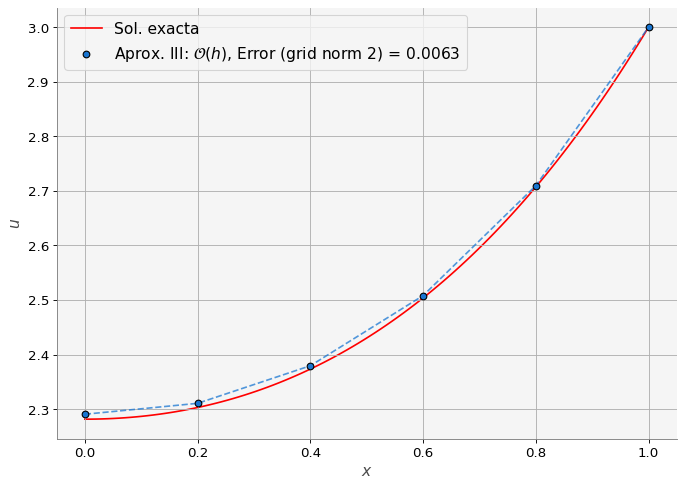
\includegraphics{02_precios_producto_files/figure-pdf/cell-21-output-1.png}

\bookmarksetup{startatroot}

\chapter{Análisis de precios de un producto: graficas para
presentación.}\label{anuxe1lisis-de-precios-de-un-producto-graficas-para-presentaciuxf3n.}

HeCompA - Precios-Producto by Luis M. de la Cruz is licensed under
Attribution-ShareAlike 4.0 International

\textbf{Trabajo realizado con el apoyo del Programa UNAM-DGAPA-PAPIME
PE101922}

\subsection{Contar la historia final}\label{contar-la-historia-final}

\begin{Shaded}
\begin{Highlighting}[]
\ImportTok{import}\NormalTok{ numpy }\ImportTok{as}\NormalTok{ np}
\ImportTok{import}\NormalTok{ pandas }\ImportTok{as}\NormalTok{ pd}
\ImportTok{import}\NormalTok{ matplotlib.pyplot }\ImportTok{as}\NormalTok{ plt}

\CommentTok{\# Parámetros para el estilo de las gráficas}
\NormalTok{params }\OperatorTok{=}\NormalTok{ \{}\StringTok{\textquotesingle{}figure.figsize\textquotesingle{}}\NormalTok{ : (}\DecValTok{10}\NormalTok{,}\DecValTok{5}\NormalTok{),}
          \StringTok{\textquotesingle{}xtick.labelsize\textquotesingle{}}\NormalTok{: }\DecValTok{16}\NormalTok{,}
          \StringTok{\textquotesingle{}ytick.labelsize\textquotesingle{}}\NormalTok{: }\DecValTok{16}\NormalTok{,}
          \StringTok{\textquotesingle{}axes.labelsize\textquotesingle{}}\NormalTok{ : }\DecValTok{20}\NormalTok{,}
          \StringTok{\textquotesingle{}axes.titlesize\textquotesingle{}}\NormalTok{ : }\DecValTok{20}\NormalTok{,}
          \StringTok{\textquotesingle{}legend.fontsize\textquotesingle{}}\NormalTok{: }\DecValTok{14}\NormalTok{,}
          \StringTok{\textquotesingle{}grid.color\textquotesingle{}}\NormalTok{     : }\StringTok{\textquotesingle{}darkgray\textquotesingle{}}\NormalTok{,}
          \StringTok{\textquotesingle{}grid.linewidth\textquotesingle{}}\NormalTok{ : }\FloatTok{0.5}\NormalTok{,}
          \StringTok{\textquotesingle{}grid.linestyle\textquotesingle{}}\NormalTok{ : }\StringTok{\textquotesingle{}{-}{-}\textquotesingle{}}\NormalTok{,}
          \StringTok{\textquotesingle{}font.family\textquotesingle{}}\NormalTok{: }\StringTok{\textquotesingle{}DejaVu Serif\textquotesingle{}}\NormalTok{,}
\NormalTok{         \}}
\NormalTok{plt.rcParams.update(params)}
\end{Highlighting}
\end{Shaded}

\begin{Shaded}
\begin{Highlighting}[]
\NormalTok{precios }\OperatorTok{=}\NormalTok{ pd.read\_excel(}\StringTok{"Libro1.xlsx"}\NormalTok{, index\_col}\OperatorTok{=}\DecValTok{0}\NormalTok{)}
\NormalTok{precios}
\end{Highlighting}
\end{Shaded}

\begin{longtable}[]{@{}llllllll@{}}
\toprule\noalign{}
& 2013 & 2014 & 2015 & 2016 & 2017 & 2018 & 2019 \\
\midrule\noalign{}
\endhead
\bottomrule\noalign{}
\endlastfoot
Prod A & 395.0 & 420.0 & 430.0 & 390.0 & 300.0 & 275 & 260 \\
Prod B & 370.0 & 400.0 & 405.0 & 380.0 & 295.0 & 255 & 245 \\
Prod C & NaN & NaN & 100.0 & 180.0 & 200.0 & 240 & 182 \\
Prod D & NaN & NaN & NaN & 160.0 & 265.0 & 215 & 210 \\
Prod E & NaN & NaN & NaN & NaN & NaN & 100 & 205 \\
\end{longtable}

\begin{Shaded}
\begin{Highlighting}[]
\NormalTok{A }\OperatorTok{=}\NormalTok{ np.array(precios.iloc[}\DecValTok{0}\NormalTok{])}
\NormalTok{B }\OperatorTok{=}\NormalTok{ np.array(precios.iloc[}\DecValTok{1}\NormalTok{])}
\NormalTok{C }\OperatorTok{=}\NormalTok{ np.array(precios.iloc[}\DecValTok{2}\NormalTok{])}
\NormalTok{D }\OperatorTok{=}\NormalTok{ np.array(precios.iloc[}\DecValTok{3}\NormalTok{])}
\NormalTok{E }\OperatorTok{=}\NormalTok{ np.array(precios.iloc[}\DecValTok{4}\NormalTok{])}
\BuiltInTok{print}\NormalTok{(A)}
\BuiltInTok{print}\NormalTok{(B)}
\BuiltInTok{print}\NormalTok{(C)}
\BuiltInTok{print}\NormalTok{(D)}
\BuiltInTok{print}\NormalTok{(E)}
\end{Highlighting}
\end{Shaded}

\begin{verbatim}
[395. 420. 430. 390. 300. 275. 260.]
[370. 400. 405. 380. 295. 255. 245.]
[ nan  nan 100. 180. 200. 240. 182.]
[ nan  nan  nan 160. 265. 215. 210.]
[ nan  nan  nan  nan  nan 100. 205.]
\end{verbatim}

\begin{Shaded}
\begin{Highlighting}[]
\CommentTok{\# Arreglo para usarse en el eje x}
\NormalTok{x2 }\OperatorTok{=}\NormalTok{ np.arange(}\DecValTok{2013}\NormalTok{,}\DecValTok{2020}\NormalTok{,}\DecValTok{1}\NormalTok{)}
\NormalTok{x2}
\end{Highlighting}
\end{Shaded}

\begin{verbatim}
array([2013, 2014, 2015, 2016, 2017, 2018, 2019])
\end{verbatim}

\begin{Shaded}
\begin{Highlighting}[]
\NormalTok{fig }\OperatorTok{=}\NormalTok{ plt.figure() }\CommentTok{\# Se define una figura}
\NormalTok{ax }\OperatorTok{=}\NormalTok{ fig.gca()     }\CommentTok{\# Se obtienen los ejes de la figura}

\CommentTok{\# Producto A}
\NormalTok{ax.scatter(x2[}\DecValTok{0}\NormalTok{], A[}\DecValTok{0}\NormalTok{], marker}\OperatorTok{=}\StringTok{\textquotesingle{}o\textquotesingle{}}\NormalTok{, alpha}\OperatorTok{=}\FloatTok{0.85}\NormalTok{, ec }\OperatorTok{=} \StringTok{\textquotesingle{}k\textquotesingle{}}\NormalTok{, s}\OperatorTok{=}\DecValTok{75}\NormalTok{, zorder}\OperatorTok{=}\DecValTok{5}\NormalTok{, color}\OperatorTok{=}\StringTok{\textquotesingle{}royalblue\textquotesingle{}}\NormalTok{)}

\CommentTok{\# Producto B}
\NormalTok{ax.scatter(x2[}\DecValTok{0}\NormalTok{], B[}\DecValTok{0}\NormalTok{], marker}\OperatorTok{=}\StringTok{\textquotesingle{}o\textquotesingle{}}\NormalTok{, alpha}\OperatorTok{=}\FloatTok{0.85}\NormalTok{, ec }\OperatorTok{=} \StringTok{\textquotesingle{}k\textquotesingle{}}\NormalTok{, s}\OperatorTok{=}\DecValTok{75}\NormalTok{, zorder}\OperatorTok{=}\DecValTok{5}\NormalTok{, color}\OperatorTok{=}\StringTok{\textquotesingle{}royalblue\textquotesingle{}}\NormalTok{)}

\CommentTok{\# Límites en el eje y}
\NormalTok{ax.set\_ylim(}\DecValTok{0}\NormalTok{,}\DecValTok{500}\NormalTok{)}
\NormalTok{ax.set\_xlim(}\FloatTok{2012.5}\NormalTok{,}\FloatTok{2019.5}\NormalTok{)}

\CommentTok{\# Marcas sobre los ejes (ojo: ya no hacen falta los xticks)}
\NormalTok{ax.set\_xticks(ticks}\OperatorTok{=}\NormalTok{[i }\ControlFlowTok{for}\NormalTok{ i }\KeywordTok{in} \BuiltInTok{range}\NormalTok{(}\DecValTok{2013}\NormalTok{,}\DecValTok{2020}\NormalTok{)])}
\NormalTok{ax.set\_yticks(ticks}\OperatorTok{=}\NormalTok{[}\DecValTok{0}\NormalTok{,}\DecValTok{100}\NormalTok{,}\DecValTok{200}\NormalTok{,}\DecValTok{300}\NormalTok{,}\DecValTok{400}\NormalTok{,}\DecValTok{500}\NormalTok{], }
\NormalTok{              labels}\OperatorTok{=}\NormalTok{[}\StringTok{\textquotesingle{}\textbackslash{}$0\textquotesingle{}}\NormalTok{,}\StringTok{\textquotesingle{}\textbackslash{}$100\textquotesingle{}}\NormalTok{,}\StringTok{\textquotesingle{}\textbackslash{}$200\textquotesingle{}}\NormalTok{,}\StringTok{\textquotesingle{}\textbackslash{}$300\textquotesingle{}}\NormalTok{,}\StringTok{\textquotesingle{}\textbackslash{}$400\textquotesingle{}}\NormalTok{,}\StringTok{\textquotesingle{}\textbackslash{}$500\textquotesingle{}}\NormalTok{])}

\CommentTok{\# Rejilla}
\NormalTok{ax.grid()}

\NormalTok{ax.text(x }\OperatorTok{=}\NormalTok{ x2[}\DecValTok{0}\NormalTok{]}\OperatorTok{{-}}\FloatTok{0.20}\NormalTok{, y }\OperatorTok{=}\NormalTok{ A[}\DecValTok{0}\NormalTok{], s }\OperatorTok{=} \StringTok{\textquotesingle{}A\textquotesingle{}}\NormalTok{, fontsize }\OperatorTok{=} \DecValTok{18}\NormalTok{)}
\NormalTok{ax.text(x }\OperatorTok{=}\NormalTok{ x2[}\DecValTok{0}\NormalTok{]}\OperatorTok{{-}}\FloatTok{0.20}\NormalTok{, y }\OperatorTok{=}\NormalTok{ B[}\DecValTok{0}\NormalTok{]}\OperatorTok{{-}}\DecValTok{20}\NormalTok{, s }\OperatorTok{=} \StringTok{\textquotesingle{}B\textquotesingle{}}\NormalTok{, fontsize }\OperatorTok{=} \DecValTok{18}\NormalTok{)}

\NormalTok{ax.spines[}\StringTok{\textquotesingle{}right\textquotesingle{}}\NormalTok{].set\_visible(}\VariableTok{False}\NormalTok{)}
\NormalTok{ax.spines[}\StringTok{\textquotesingle{}top\textquotesingle{}}\NormalTok{].set\_visible(}\VariableTok{False}\NormalTok{)}
\NormalTok{ax.spines[}\StringTok{\textquotesingle{}left\textquotesingle{}}\NormalTok{].set\_color(}\StringTok{\textquotesingle{}gray\textquotesingle{}}\NormalTok{)}
\NormalTok{ax.spines[}\StringTok{\textquotesingle{}bottom\textquotesingle{}}\NormalTok{].set\_color(}\StringTok{\textquotesingle{}gray\textquotesingle{}}\NormalTok{)}
\NormalTok{ax.tick\_params(axis}\OperatorTok{=}\StringTok{\textquotesingle{}x\textquotesingle{}}\NormalTok{, colors}\OperatorTok{=}\StringTok{\textquotesingle{}\#444444\textquotesingle{}}\NormalTok{)}
\NormalTok{ax.tick\_params(axis}\OperatorTok{=}\StringTok{\textquotesingle{}y\textquotesingle{}}\NormalTok{, colors}\OperatorTok{=}\StringTok{\textquotesingle{}\#444444\textquotesingle{}}\NormalTok{)}

\NormalTok{plt.suptitle(}\StringTok{\textquotesingle{}Precio promedio por año\textquotesingle{}}\NormalTok{, fontsize}\OperatorTok{=}\DecValTok{24}\NormalTok{, x }\OperatorTok{=}\FloatTok{0.275}\NormalTok{, y}\OperatorTok{=}\FloatTok{1.05}\NormalTok{)}
\NormalTok{plt.savefig(}\StringTok{\textquotesingle{}vis1.png\textquotesingle{}}\NormalTok{,bbox\_inches}\OperatorTok{=}\StringTok{\textquotesingle{}tight\textquotesingle{}}\NormalTok{, dpi}\OperatorTok{=}\DecValTok{150}\NormalTok{)}
\NormalTok{plt.show()}
\end{Highlighting}
\end{Shaded}

\includegraphics{03_precios_graficas_storytelling_files/figure-pdf/cell-6-output-1.png}

\begin{Shaded}
\begin{Highlighting}[]
\CommentTok{\# Visualización 12: usamos líneas con color}
\NormalTok{fig }\OperatorTok{=}\NormalTok{ plt.figure() }\CommentTok{\# Se define una figura}
\NormalTok{ax }\OperatorTok{=}\NormalTok{ fig.gca()     }\CommentTok{\# Se obtienen los ejes de la figura}

\CommentTok{\# Producto A}
\NormalTok{ax.plot(x2, A, lw}\OperatorTok{=}\DecValTok{3}\NormalTok{, c}\OperatorTok{=}\StringTok{\textquotesingle{}darkgray\textquotesingle{}}\NormalTok{)}
\NormalTok{ax.scatter(x2[}\DecValTok{0}\NormalTok{], A[}\DecValTok{0}\NormalTok{], marker}\OperatorTok{=}\StringTok{\textquotesingle{}o\textquotesingle{}}\NormalTok{, alpha}\OperatorTok{=}\FloatTok{0.85}\NormalTok{, ec }\OperatorTok{=} \StringTok{\textquotesingle{}k\textquotesingle{}}\NormalTok{, s}\OperatorTok{=}\DecValTok{75}\NormalTok{, zorder}\OperatorTok{=}\DecValTok{5}\NormalTok{, color}\OperatorTok{=}\StringTok{\textquotesingle{}royalblue\textquotesingle{}}\NormalTok{)}
\NormalTok{ax.scatter(x2[}\OperatorTok{{-}}\DecValTok{1}\NormalTok{], A[}\OperatorTok{{-}}\DecValTok{1}\NormalTok{], marker}\OperatorTok{=}\StringTok{\textquotesingle{}o\textquotesingle{}}\NormalTok{, alpha}\OperatorTok{=}\FloatTok{0.85}\NormalTok{, ec }\OperatorTok{=} \StringTok{\textquotesingle{}k\textquotesingle{}}\NormalTok{, s}\OperatorTok{=}\DecValTok{75}\NormalTok{, zorder}\OperatorTok{=}\DecValTok{5}\NormalTok{, color}\OperatorTok{=}\StringTok{\textquotesingle{}forestgreen\textquotesingle{}}\NormalTok{)}

\CommentTok{\# Producto B}
\NormalTok{ax.plot(x2, B, lw}\OperatorTok{=}\DecValTok{3}\NormalTok{, c}\OperatorTok{=}\StringTok{\textquotesingle{}darkgray\textquotesingle{}}\NormalTok{)}
\NormalTok{ax.scatter(x2[}\DecValTok{0}\NormalTok{], B[}\DecValTok{0}\NormalTok{], marker}\OperatorTok{=}\StringTok{\textquotesingle{}o\textquotesingle{}}\NormalTok{, alpha}\OperatorTok{=}\FloatTok{0.85}\NormalTok{, ec }\OperatorTok{=} \StringTok{\textquotesingle{}k\textquotesingle{}}\NormalTok{, s}\OperatorTok{=}\DecValTok{75}\NormalTok{, zorder}\OperatorTok{=}\DecValTok{5}\NormalTok{, color}\OperatorTok{=}\StringTok{\textquotesingle{}royalblue\textquotesingle{}}\NormalTok{)}
\NormalTok{ax.scatter(x2[}\OperatorTok{{-}}\DecValTok{1}\NormalTok{], B[}\OperatorTok{{-}}\DecValTok{1}\NormalTok{], marker}\OperatorTok{=}\StringTok{\textquotesingle{}o\textquotesingle{}}\NormalTok{, alpha}\OperatorTok{=}\FloatTok{0.85}\NormalTok{, ec }\OperatorTok{=} \StringTok{\textquotesingle{}k\textquotesingle{}}\NormalTok{, s}\OperatorTok{=}\DecValTok{75}\NormalTok{, zorder}\OperatorTok{=}\DecValTok{5}\NormalTok{, color}\OperatorTok{=}\StringTok{\textquotesingle{}forestgreen\textquotesingle{}}\NormalTok{)}

\CommentTok{\# Límites en el eje y}
\NormalTok{ax.set\_ylim(}\DecValTok{0}\NormalTok{,}\DecValTok{500}\NormalTok{)}
\NormalTok{ax.set\_xlim(}\FloatTok{2012.5}\NormalTok{,}\FloatTok{2019.5}\NormalTok{)}

\CommentTok{\# Marcas sobre los ejes (ojo: ya no hacen falta los xticks)}
\NormalTok{ax.set\_xticks(ticks}\OperatorTok{=}\NormalTok{[i }\ControlFlowTok{for}\NormalTok{ i }\KeywordTok{in} \BuiltInTok{range}\NormalTok{(}\DecValTok{2013}\NormalTok{,}\DecValTok{2020}\NormalTok{)])}
\NormalTok{ax.set\_yticks(ticks}\OperatorTok{=}\NormalTok{[}\DecValTok{0}\NormalTok{,}\DecValTok{100}\NormalTok{,}\DecValTok{200}\NormalTok{,}\DecValTok{300}\NormalTok{,}\DecValTok{400}\NormalTok{,}\DecValTok{500}\NormalTok{], }
\NormalTok{              labels}\OperatorTok{=}\NormalTok{[}\StringTok{\textquotesingle{}\textbackslash{}$0\textquotesingle{}}\NormalTok{,}\StringTok{\textquotesingle{}\textbackslash{}$100\textquotesingle{}}\NormalTok{,}\StringTok{\textquotesingle{}\textbackslash{}$200\textquotesingle{}}\NormalTok{,}\StringTok{\textquotesingle{}\textbackslash{}$300\textquotesingle{}}\NormalTok{,}\StringTok{\textquotesingle{}\textbackslash{}$400\textquotesingle{}}\NormalTok{,}\StringTok{\textquotesingle{}\textbackslash{}$500\textquotesingle{}}\NormalTok{])}

\CommentTok{\# Rejilla}
\NormalTok{ax.grid()}

\NormalTok{ax.text(x }\OperatorTok{=}\NormalTok{ x2[}\DecValTok{0}\NormalTok{]}\OperatorTok{{-}}\FloatTok{0.20}\NormalTok{, y }\OperatorTok{=}\NormalTok{ A[}\DecValTok{0}\NormalTok{], s }\OperatorTok{=} \StringTok{\textquotesingle{}A\textquotesingle{}}\NormalTok{, fontsize }\OperatorTok{=} \DecValTok{18}\NormalTok{)}
\NormalTok{ax.text(x }\OperatorTok{=}\NormalTok{ x2[}\DecValTok{0}\NormalTok{]}\OperatorTok{{-}}\FloatTok{0.20}\NormalTok{, y }\OperatorTok{=}\NormalTok{ B[}\DecValTok{0}\NormalTok{]}\OperatorTok{{-}}\DecValTok{20}\NormalTok{, s }\OperatorTok{=} \StringTok{\textquotesingle{}B\textquotesingle{}}\NormalTok{, fontsize }\OperatorTok{=} \DecValTok{18}\NormalTok{)}

\NormalTok{ax.spines[}\StringTok{\textquotesingle{}right\textquotesingle{}}\NormalTok{].set\_visible(}\VariableTok{False}\NormalTok{)}
\NormalTok{ax.spines[}\StringTok{\textquotesingle{}top\textquotesingle{}}\NormalTok{].set\_visible(}\VariableTok{False}\NormalTok{)}
\NormalTok{ax.spines[}\StringTok{\textquotesingle{}left\textquotesingle{}}\NormalTok{].set\_color(}\StringTok{\textquotesingle{}gray\textquotesingle{}}\NormalTok{)}
\NormalTok{ax.spines[}\StringTok{\textquotesingle{}bottom\textquotesingle{}}\NormalTok{].set\_color(}\StringTok{\textquotesingle{}gray\textquotesingle{}}\NormalTok{)}
\NormalTok{ax.tick\_params(axis}\OperatorTok{=}\StringTok{\textquotesingle{}x\textquotesingle{}}\NormalTok{, colors}\OperatorTok{=}\StringTok{\textquotesingle{}\#444444\textquotesingle{}}\NormalTok{)}
\NormalTok{ax.tick\_params(axis}\OperatorTok{=}\StringTok{\textquotesingle{}y\textquotesingle{}}\NormalTok{, colors}\OperatorTok{=}\StringTok{\textquotesingle{}\#444444\textquotesingle{}}\NormalTok{)}

\NormalTok{plt.suptitle(}\StringTok{\textquotesingle{}Precio promedio por año\textquotesingle{}}\NormalTok{, fontsize}\OperatorTok{=}\DecValTok{24}\NormalTok{, x }\OperatorTok{=}\FloatTok{0.275}\NormalTok{, y}\OperatorTok{=}\FloatTok{1.05}\NormalTok{)}
\NormalTok{plt.savefig(}\StringTok{\textquotesingle{}vis2.png\textquotesingle{}}\NormalTok{,bbox\_inches}\OperatorTok{=}\StringTok{\textquotesingle{}tight\textquotesingle{}}\NormalTok{, dpi}\OperatorTok{=}\DecValTok{150}\NormalTok{)}
\NormalTok{plt.show()}
\end{Highlighting}
\end{Shaded}

\includegraphics{03_precios_graficas_storytelling_files/figure-pdf/cell-7-output-1.png}

\begin{Shaded}
\begin{Highlighting}[]
\NormalTok{fig }\OperatorTok{=}\NormalTok{ plt.figure() }\CommentTok{\# Se define una figura}
\NormalTok{ax }\OperatorTok{=}\NormalTok{ fig.gca()     }\CommentTok{\# Se obtienen los ejes de la figura}

\CommentTok{\# Producto A}
\NormalTok{ax.plot(x2, A, lw}\OperatorTok{=}\DecValTok{3}\NormalTok{, c}\OperatorTok{=}\StringTok{\textquotesingle{}darkgray\textquotesingle{}}\NormalTok{)}
\NormalTok{ax.scatter(x2[}\DecValTok{0}\NormalTok{], A[}\DecValTok{0}\NormalTok{], marker}\OperatorTok{=}\StringTok{\textquotesingle{}o\textquotesingle{}}\NormalTok{, alpha}\OperatorTok{=}\FloatTok{0.85}\NormalTok{, ec }\OperatorTok{=} \StringTok{\textquotesingle{}k\textquotesingle{}}\NormalTok{, s}\OperatorTok{=}\DecValTok{75}\NormalTok{, zorder}\OperatorTok{=}\DecValTok{5}\NormalTok{, color}\OperatorTok{=}\StringTok{\textquotesingle{}royalblue\textquotesingle{}}\NormalTok{)}

\CommentTok{\# Producto B}
\NormalTok{ax.plot(x2, B, lw}\OperatorTok{=}\DecValTok{3}\NormalTok{, c}\OperatorTok{=}\StringTok{\textquotesingle{}darkgray\textquotesingle{}}\NormalTok{)}
\NormalTok{ax.scatter(x2[}\DecValTok{0}\NormalTok{], B[}\DecValTok{0}\NormalTok{], marker}\OperatorTok{=}\StringTok{\textquotesingle{}o\textquotesingle{}}\NormalTok{, alpha}\OperatorTok{=}\FloatTok{0.85}\NormalTok{, ec }\OperatorTok{=} \StringTok{\textquotesingle{}k\textquotesingle{}}\NormalTok{, s}\OperatorTok{=}\DecValTok{75}\NormalTok{, zorder}\OperatorTok{=}\DecValTok{5}\NormalTok{, color}\OperatorTok{=}\StringTok{\textquotesingle{}royalblue\textquotesingle{}}\NormalTok{)}

\CommentTok{\# Producto C}
\NormalTok{ax.scatter(x2[}\DecValTok{2}\NormalTok{], C[}\DecValTok{2}\NormalTok{], marker}\OperatorTok{=}\StringTok{\textquotesingle{}o\textquotesingle{}}\NormalTok{, alpha}\OperatorTok{=}\FloatTok{0.85}\NormalTok{, ec }\OperatorTok{=} \StringTok{\textquotesingle{}k\textquotesingle{}}\NormalTok{, s}\OperatorTok{=}\DecValTok{75}\NormalTok{, zorder}\OperatorTok{=}\DecValTok{5}\NormalTok{, color}\OperatorTok{=}\StringTok{\textquotesingle{}royalblue\textquotesingle{}}\NormalTok{)}

\CommentTok{\# Producto D}
\NormalTok{ax.scatter(x2[}\DecValTok{3}\NormalTok{], D[}\DecValTok{3}\NormalTok{], marker}\OperatorTok{=}\StringTok{\textquotesingle{}o\textquotesingle{}}\NormalTok{, alpha}\OperatorTok{=}\FloatTok{0.85}\NormalTok{, ec }\OperatorTok{=} \StringTok{\textquotesingle{}k\textquotesingle{}}\NormalTok{, s}\OperatorTok{=}\DecValTok{75}\NormalTok{, zorder}\OperatorTok{=}\DecValTok{5}\NormalTok{, color}\OperatorTok{=}\StringTok{\textquotesingle{}royalblue\textquotesingle{}}\NormalTok{)}

\CommentTok{\# Producto E}
\NormalTok{ax.scatter(x2[}\DecValTok{5}\NormalTok{], E[}\DecValTok{5}\NormalTok{], marker}\OperatorTok{=}\StringTok{\textquotesingle{}o\textquotesingle{}}\NormalTok{, alpha}\OperatorTok{=}\FloatTok{0.85}\NormalTok{, ec }\OperatorTok{=} \StringTok{\textquotesingle{}k\textquotesingle{}}\NormalTok{, s}\OperatorTok{=}\DecValTok{75}\NormalTok{, zorder}\OperatorTok{=}\DecValTok{5}\NormalTok{, color}\OperatorTok{=}\StringTok{\textquotesingle{}royalblue\textquotesingle{}}\NormalTok{)}

\CommentTok{\# Límites en los ejes}
\NormalTok{ax.set\_ylim(}\DecValTok{0}\NormalTok{,}\DecValTok{500}\NormalTok{)}
\NormalTok{ax.set\_xlim(}\FloatTok{2012.5}\NormalTok{,}\FloatTok{2019.5}\NormalTok{)}

\CommentTok{\# Marcas sobre los ejes}
\NormalTok{ax.set\_xticks(ticks}\OperatorTok{=}\NormalTok{[i }\ControlFlowTok{for}\NormalTok{ i }\KeywordTok{in} \BuiltInTok{range}\NormalTok{(}\DecValTok{2013}\NormalTok{,}\DecValTok{2020}\NormalTok{)])}
\NormalTok{ax.set\_yticks(ticks}\OperatorTok{=}\NormalTok{[}\DecValTok{0}\NormalTok{,}\DecValTok{100}\NormalTok{,}\DecValTok{200}\NormalTok{,}\DecValTok{300}\NormalTok{,}\DecValTok{400}\NormalTok{,}\DecValTok{500}\NormalTok{], }
\NormalTok{              labels}\OperatorTok{=}\NormalTok{[}\StringTok{\textquotesingle{}\textbackslash{}$0\textquotesingle{}}\NormalTok{,}\StringTok{\textquotesingle{}\textbackslash{}$100\textquotesingle{}}\NormalTok{,}\StringTok{\textquotesingle{}\textbackslash{}$200\textquotesingle{}}\NormalTok{,}\StringTok{\textquotesingle{}\textbackslash{}$300\textquotesingle{}}\NormalTok{,}\StringTok{\textquotesingle{}\textbackslash{}$400\textquotesingle{}}\NormalTok{,}\StringTok{\textquotesingle{}\textbackslash{}$500\textquotesingle{}}\NormalTok{])}

\CommentTok{\# Rejilla}
\NormalTok{ax.grid()}

\NormalTok{ax.text(x }\OperatorTok{=}\NormalTok{ x2[}\DecValTok{0}\NormalTok{]}\OperatorTok{{-}}\FloatTok{0.20}\NormalTok{, y }\OperatorTok{=}\NormalTok{ A[}\DecValTok{0}\NormalTok{], s }\OperatorTok{=} \StringTok{\textquotesingle{}A\textquotesingle{}}\NormalTok{, fontsize }\OperatorTok{=} \DecValTok{18}\NormalTok{)}
\NormalTok{ax.text(x }\OperatorTok{=}\NormalTok{ x2[}\DecValTok{0}\NormalTok{]}\OperatorTok{{-}}\FloatTok{0.20}\NormalTok{, y }\OperatorTok{=}\NormalTok{ B[}\DecValTok{0}\NormalTok{]}\OperatorTok{{-}}\DecValTok{20}\NormalTok{, s }\OperatorTok{=} \StringTok{\textquotesingle{}B\textquotesingle{}}\NormalTok{, fontsize }\OperatorTok{=} \DecValTok{18}\NormalTok{)}
\NormalTok{ax.text(x }\OperatorTok{=}\NormalTok{ x2[}\DecValTok{2}\NormalTok{]}\OperatorTok{{-}}\FloatTok{0.20}\NormalTok{, y }\OperatorTok{=}\NormalTok{ C[}\DecValTok{2}\NormalTok{]}\OperatorTok{{-}}\DecValTok{20}\NormalTok{, s }\OperatorTok{=} \StringTok{\textquotesingle{}C\textquotesingle{}}\NormalTok{, fontsize }\OperatorTok{=} \DecValTok{18}\NormalTok{)}
\NormalTok{ax.text(x }\OperatorTok{=}\NormalTok{ x2[}\DecValTok{3}\NormalTok{]}\OperatorTok{{-}}\FloatTok{0.20}\NormalTok{, y }\OperatorTok{=}\NormalTok{ D[}\DecValTok{3}\NormalTok{]}\OperatorTok{{-}}\DecValTok{20}\NormalTok{, s }\OperatorTok{=} \StringTok{\textquotesingle{}D\textquotesingle{}}\NormalTok{, fontsize }\OperatorTok{=} \DecValTok{18}\NormalTok{)}
\NormalTok{ax.text(x }\OperatorTok{=}\NormalTok{ x2[}\DecValTok{5}\NormalTok{]}\OperatorTok{{-}}\FloatTok{0.20}\NormalTok{, y }\OperatorTok{=}\NormalTok{ E[}\DecValTok{5}\NormalTok{]}\OperatorTok{{-}}\DecValTok{20}\NormalTok{, s }\OperatorTok{=} \StringTok{\textquotesingle{}E\textquotesingle{}}\NormalTok{, fontsize }\OperatorTok{=} \DecValTok{18}\NormalTok{)}

\NormalTok{ax.spines[}\StringTok{\textquotesingle{}right\textquotesingle{}}\NormalTok{].set\_visible(}\VariableTok{False}\NormalTok{)}
\NormalTok{ax.spines[}\StringTok{\textquotesingle{}top\textquotesingle{}}\NormalTok{].set\_visible(}\VariableTok{False}\NormalTok{)}
\NormalTok{ax.spines[}\StringTok{\textquotesingle{}left\textquotesingle{}}\NormalTok{].set\_color(}\StringTok{\textquotesingle{}gray\textquotesingle{}}\NormalTok{)}
\NormalTok{ax.spines[}\StringTok{\textquotesingle{}bottom\textquotesingle{}}\NormalTok{].set\_color(}\StringTok{\textquotesingle{}gray\textquotesingle{}}\NormalTok{)}
\NormalTok{ax.tick\_params(axis}\OperatorTok{=}\StringTok{\textquotesingle{}x\textquotesingle{}}\NormalTok{, colors}\OperatorTok{=}\StringTok{\textquotesingle{}\#444444\textquotesingle{}}\NormalTok{)}
\NormalTok{ax.tick\_params(axis}\OperatorTok{=}\StringTok{\textquotesingle{}y\textquotesingle{}}\NormalTok{, colors}\OperatorTok{=}\StringTok{\textquotesingle{}\#444444\textquotesingle{}}\NormalTok{)}

\NormalTok{plt.suptitle(}\StringTok{\textquotesingle{}Precio promedio por año\textquotesingle{}}\NormalTok{, fontsize}\OperatorTok{=}\DecValTok{24}\NormalTok{, x }\OperatorTok{=}\FloatTok{0.275}\NormalTok{, y}\OperatorTok{=}\FloatTok{1.05}\NormalTok{)}
\NormalTok{plt.savefig(}\StringTok{\textquotesingle{}vis3.png\textquotesingle{}}\NormalTok{,bbox\_inches}\OperatorTok{=}\StringTok{\textquotesingle{}tight\textquotesingle{}}\NormalTok{, dpi}\OperatorTok{=}\DecValTok{150}\NormalTok{)}
\NormalTok{plt.show()}
\end{Highlighting}
\end{Shaded}

\includegraphics{03_precios_graficas_storytelling_files/figure-pdf/cell-8-output-1.png}

\begin{Shaded}
\begin{Highlighting}[]
\CommentTok{\# Visualización 8: usamos líneas con color}
\NormalTok{fig }\OperatorTok{=}\NormalTok{ plt.figure() }\CommentTok{\# Se define una figura}
\NormalTok{ax }\OperatorTok{=}\NormalTok{ fig.gca()     }\CommentTok{\# Se obtienen los ejes de la figura}

\CommentTok{\# Producto A}
\NormalTok{ax.plot(x2[}\DecValTok{0}\NormalTok{:}\DecValTok{3}\NormalTok{], A[}\DecValTok{0}\NormalTok{:}\DecValTok{3}\NormalTok{], lw}\OperatorTok{=}\DecValTok{3}\NormalTok{, color}\OperatorTok{=}\StringTok{\textquotesingle{}firebrick\textquotesingle{}}\NormalTok{)}
\NormalTok{ax.scatter(x2[}\DecValTok{0}\NormalTok{], A[}\DecValTok{0}\NormalTok{], marker}\OperatorTok{=}\StringTok{\textquotesingle{}o\textquotesingle{}}\NormalTok{, alpha}\OperatorTok{=}\FloatTok{0.85}\NormalTok{, ec }\OperatorTok{=} \StringTok{\textquotesingle{}k\textquotesingle{}}\NormalTok{, s}\OperatorTok{=}\DecValTok{75}\NormalTok{, zorder}\OperatorTok{=}\DecValTok{5}\NormalTok{, color}\OperatorTok{=}\StringTok{\textquotesingle{}royalblue\textquotesingle{}}\NormalTok{)}

\CommentTok{\# Producto B}
\NormalTok{ax.plot(x2[}\DecValTok{0}\NormalTok{:}\DecValTok{3}\NormalTok{], B[}\DecValTok{0}\NormalTok{:}\DecValTok{3}\NormalTok{], lw}\OperatorTok{=}\DecValTok{3}\NormalTok{, color}\OperatorTok{=}\StringTok{\textquotesingle{}firebrick\textquotesingle{}}\NormalTok{)}
\NormalTok{ax.scatter(x2[}\DecValTok{0}\NormalTok{], B[}\DecValTok{0}\NormalTok{], marker}\OperatorTok{=}\StringTok{\textquotesingle{}o\textquotesingle{}}\NormalTok{, alpha}\OperatorTok{=}\FloatTok{0.85}\NormalTok{, ec }\OperatorTok{=} \StringTok{\textquotesingle{}k\textquotesingle{}}\NormalTok{, s}\OperatorTok{=}\DecValTok{75}\NormalTok{, zorder}\OperatorTok{=}\DecValTok{5}\NormalTok{, color}\OperatorTok{=}\StringTok{\textquotesingle{}royalblue\textquotesingle{}}\NormalTok{)}

\CommentTok{\# Producto C}
\NormalTok{ax.plot(x2[}\DecValTok{2}\NormalTok{:}\DecValTok{6}\NormalTok{], C[}\DecValTok{2}\NormalTok{:}\DecValTok{6}\NormalTok{], lw}\OperatorTok{=}\DecValTok{3}\NormalTok{, color}\OperatorTok{=}\StringTok{\textquotesingle{}firebrick\textquotesingle{}}\NormalTok{)}
\NormalTok{ax.scatter(x2[}\DecValTok{2}\NormalTok{], C[}\DecValTok{2}\NormalTok{], marker}\OperatorTok{=}\StringTok{\textquotesingle{}o\textquotesingle{}}\NormalTok{, alpha}\OperatorTok{=}\FloatTok{0.85}\NormalTok{, ec }\OperatorTok{=} \StringTok{\textquotesingle{}k\textquotesingle{}}\NormalTok{, s}\OperatorTok{=}\DecValTok{75}\NormalTok{, zorder}\OperatorTok{=}\DecValTok{5}\NormalTok{, color}\OperatorTok{=}\StringTok{\textquotesingle{}royalblue\textquotesingle{}}\NormalTok{)}

\CommentTok{\# Producto D}
\NormalTok{ax.plot(x2[}\DecValTok{3}\NormalTok{:}\DecValTok{5}\NormalTok{], D[}\DecValTok{3}\NormalTok{:}\DecValTok{5}\NormalTok{], lw}\OperatorTok{=}\DecValTok{3}\NormalTok{, color}\OperatorTok{=}\StringTok{\textquotesingle{}firebrick\textquotesingle{}}\NormalTok{)}
\NormalTok{ax.scatter(x2[}\DecValTok{3}\NormalTok{], D[}\DecValTok{3}\NormalTok{], marker}\OperatorTok{=}\StringTok{\textquotesingle{}o\textquotesingle{}}\NormalTok{, alpha}\OperatorTok{=}\FloatTok{0.85}\NormalTok{, ec }\OperatorTok{=} \StringTok{\textquotesingle{}k\textquotesingle{}}\NormalTok{, s}\OperatorTok{=}\DecValTok{75}\NormalTok{, zorder}\OperatorTok{=}\DecValTok{5}\NormalTok{, color}\OperatorTok{=}\StringTok{\textquotesingle{}royalblue\textquotesingle{}}\NormalTok{)}

\CommentTok{\# Producto E}
\NormalTok{ax.plot(x2, E, lw}\OperatorTok{=}\DecValTok{3}\NormalTok{, c}\OperatorTok{=}\StringTok{\textquotesingle{}firebrick\textquotesingle{}}\NormalTok{)}
\NormalTok{ax.scatter(x2[}\DecValTok{5}\NormalTok{], E[}\DecValTok{5}\NormalTok{], marker}\OperatorTok{=}\StringTok{\textquotesingle{}o\textquotesingle{}}\NormalTok{, alpha}\OperatorTok{=}\FloatTok{0.85}\NormalTok{, ec }\OperatorTok{=} \StringTok{\textquotesingle{}k\textquotesingle{}}\NormalTok{, s}\OperatorTok{=}\DecValTok{75}\NormalTok{, zorder}\OperatorTok{=}\DecValTok{5}\NormalTok{, color}\OperatorTok{=}\StringTok{\textquotesingle{}royalblue\textquotesingle{}}\NormalTok{)}

\CommentTok{\# Límites en los ejes}
\NormalTok{ax.set\_ylim(}\DecValTok{0}\NormalTok{,}\DecValTok{500}\NormalTok{)}
\NormalTok{ax.set\_xlim(}\FloatTok{2012.5}\NormalTok{,}\FloatTok{2019.5}\NormalTok{)}

\CommentTok{\# Marcas sobre los ejes}
\NormalTok{ax.set\_xticks(ticks}\OperatorTok{=}\NormalTok{[i }\ControlFlowTok{for}\NormalTok{ i }\KeywordTok{in} \BuiltInTok{range}\NormalTok{(}\DecValTok{2013}\NormalTok{,}\DecValTok{2020}\NormalTok{)])}
\NormalTok{ax.set\_yticks(ticks}\OperatorTok{=}\NormalTok{[}\DecValTok{0}\NormalTok{,}\DecValTok{100}\NormalTok{,}\DecValTok{200}\NormalTok{,}\DecValTok{300}\NormalTok{,}\DecValTok{400}\NormalTok{,}\DecValTok{500}\NormalTok{], }
\NormalTok{              labels}\OperatorTok{=}\NormalTok{[}\StringTok{\textquotesingle{}\textbackslash{}$0\textquotesingle{}}\NormalTok{,}\StringTok{\textquotesingle{}\textbackslash{}$100\textquotesingle{}}\NormalTok{,}\StringTok{\textquotesingle{}\textbackslash{}$200\textquotesingle{}}\NormalTok{,}\StringTok{\textquotesingle{}\textbackslash{}$300\textquotesingle{}}\NormalTok{,}\StringTok{\textquotesingle{}\textbackslash{}$400\textquotesingle{}}\NormalTok{,}\StringTok{\textquotesingle{}\textbackslash{}$500\textquotesingle{}}\NormalTok{])}

\CommentTok{\# Rejilla}
\NormalTok{ax.grid()}

\NormalTok{ax.text(x }\OperatorTok{=}\NormalTok{ x2[}\DecValTok{0}\NormalTok{]}\OperatorTok{{-}}\FloatTok{0.20}\NormalTok{, y }\OperatorTok{=}\NormalTok{ A[}\DecValTok{0}\NormalTok{], s }\OperatorTok{=} \StringTok{\textquotesingle{}A\textquotesingle{}}\NormalTok{, fontsize }\OperatorTok{=} \DecValTok{18}\NormalTok{)}
\NormalTok{ax.text(x }\OperatorTok{=}\NormalTok{ x2[}\DecValTok{0}\NormalTok{]}\OperatorTok{{-}}\FloatTok{0.20}\NormalTok{, y }\OperatorTok{=}\NormalTok{ B[}\DecValTok{0}\NormalTok{]}\OperatorTok{{-}}\DecValTok{20}\NormalTok{, s }\OperatorTok{=} \StringTok{\textquotesingle{}B\textquotesingle{}}\NormalTok{, fontsize }\OperatorTok{=} \DecValTok{18}\NormalTok{)}
\NormalTok{ax.text(x }\OperatorTok{=}\NormalTok{ x2[}\DecValTok{2}\NormalTok{]}\OperatorTok{{-}}\FloatTok{0.20}\NormalTok{, y }\OperatorTok{=}\NormalTok{ C[}\DecValTok{2}\NormalTok{]}\OperatorTok{{-}}\DecValTok{20}\NormalTok{, s }\OperatorTok{=} \StringTok{\textquotesingle{}C\textquotesingle{}}\NormalTok{, fontsize }\OperatorTok{=} \DecValTok{18}\NormalTok{)}
\NormalTok{ax.text(x }\OperatorTok{=}\NormalTok{ x2[}\DecValTok{3}\NormalTok{]}\OperatorTok{{-}}\FloatTok{0.20}\NormalTok{, y }\OperatorTok{=}\NormalTok{ D[}\DecValTok{3}\NormalTok{]}\OperatorTok{{-}}\DecValTok{20}\NormalTok{, s }\OperatorTok{=} \StringTok{\textquotesingle{}D\textquotesingle{}}\NormalTok{, fontsize }\OperatorTok{=} \DecValTok{18}\NormalTok{)}
\NormalTok{ax.text(x }\OperatorTok{=}\NormalTok{ x2[}\DecValTok{5}\NormalTok{]}\OperatorTok{{-}}\FloatTok{0.20}\NormalTok{, y }\OperatorTok{=}\NormalTok{ E[}\DecValTok{5}\NormalTok{]}\OperatorTok{{-}}\DecValTok{20}\NormalTok{, s }\OperatorTok{=} \StringTok{\textquotesingle{}E\textquotesingle{}}\NormalTok{, fontsize }\OperatorTok{=} \DecValTok{18}\NormalTok{)}

\NormalTok{ax.spines[}\StringTok{\textquotesingle{}right\textquotesingle{}}\NormalTok{].set\_visible(}\VariableTok{False}\NormalTok{)}
\NormalTok{ax.spines[}\StringTok{\textquotesingle{}top\textquotesingle{}}\NormalTok{].set\_visible(}\VariableTok{False}\NormalTok{)}
\NormalTok{ax.spines[}\StringTok{\textquotesingle{}left\textquotesingle{}}\NormalTok{].set\_color(}\StringTok{\textquotesingle{}gray\textquotesingle{}}\NormalTok{)}
\NormalTok{ax.spines[}\StringTok{\textquotesingle{}bottom\textquotesingle{}}\NormalTok{].set\_color(}\StringTok{\textquotesingle{}gray\textquotesingle{}}\NormalTok{)}
\NormalTok{ax.tick\_params(axis}\OperatorTok{=}\StringTok{\textquotesingle{}x\textquotesingle{}}\NormalTok{, colors}\OperatorTok{=}\StringTok{\textquotesingle{}\#444444\textquotesingle{}}\NormalTok{)}
\NormalTok{ax.tick\_params(axis}\OperatorTok{=}\StringTok{\textquotesingle{}y\textquotesingle{}}\NormalTok{, colors}\OperatorTok{=}\StringTok{\textquotesingle{}\#444444\textquotesingle{}}\NormalTok{)}

\NormalTok{plt.suptitle(}\StringTok{\textquotesingle{}Precio promedio por año\textquotesingle{}}\NormalTok{, fontsize}\OperatorTok{=}\DecValTok{24}\NormalTok{, x }\OperatorTok{=}\FloatTok{0.275}\NormalTok{, y}\OperatorTok{=}\FloatTok{1.05}\NormalTok{)}
\NormalTok{plt.savefig(}\StringTok{\textquotesingle{}vis4.png\textquotesingle{}}\NormalTok{,bbox\_inches}\OperatorTok{=}\StringTok{\textquotesingle{}tight\textquotesingle{}}\NormalTok{, dpi}\OperatorTok{=}\DecValTok{150}\NormalTok{)}
\NormalTok{plt.show()}
\end{Highlighting}
\end{Shaded}

\includegraphics{03_precios_graficas_storytelling_files/figure-pdf/cell-9-output-1.png}

\begin{Shaded}
\begin{Highlighting}[]
\NormalTok{fig }\OperatorTok{=}\NormalTok{ plt.figure() }\CommentTok{\# Se define una figura}
\NormalTok{ax }\OperatorTok{=}\NormalTok{ fig.gca()     }\CommentTok{\# Se obtienen los ejes de la figura}

\CommentTok{\# Producto A}
\NormalTok{ax.plot(x2[}\DecValTok{2}\NormalTok{:], A[}\DecValTok{2}\NormalTok{:], lw}\OperatorTok{=}\DecValTok{3}\NormalTok{, color}\OperatorTok{=}\StringTok{\textquotesingle{}royalblue\textquotesingle{}}\NormalTok{)}
\NormalTok{ax.plot(x2[}\DecValTok{0}\NormalTok{:}\DecValTok{3}\NormalTok{], A[}\DecValTok{0}\NormalTok{:}\DecValTok{3}\NormalTok{], lw}\OperatorTok{=}\DecValTok{3}\NormalTok{, color}\OperatorTok{=}\StringTok{\textquotesingle{}firebrick\textquotesingle{}}\NormalTok{)}
\NormalTok{ax.scatter(x2[}\DecValTok{0}\NormalTok{], A[}\DecValTok{0}\NormalTok{], marker}\OperatorTok{=}\StringTok{\textquotesingle{}o\textquotesingle{}}\NormalTok{, alpha}\OperatorTok{=}\FloatTok{0.85}\NormalTok{, ec }\OperatorTok{=} \StringTok{\textquotesingle{}k\textquotesingle{}}\NormalTok{, s}\OperatorTok{=}\DecValTok{75}\NormalTok{, zorder}\OperatorTok{=}\DecValTok{5}\NormalTok{, color}\OperatorTok{=}\StringTok{\textquotesingle{}royalblue\textquotesingle{}}\NormalTok{)}

\CommentTok{\# Producto B}
\NormalTok{ax.plot(x2[}\DecValTok{2}\NormalTok{:], B[}\DecValTok{2}\NormalTok{:], lw}\OperatorTok{=}\DecValTok{3}\NormalTok{, color}\OperatorTok{=}\StringTok{\textquotesingle{}royalblue\textquotesingle{}}\NormalTok{)}
\NormalTok{ax.plot(x2[}\DecValTok{0}\NormalTok{:}\DecValTok{3}\NormalTok{], B[}\DecValTok{0}\NormalTok{:}\DecValTok{3}\NormalTok{], lw}\OperatorTok{=}\DecValTok{3}\NormalTok{, color}\OperatorTok{=}\StringTok{\textquotesingle{}firebrick\textquotesingle{}}\NormalTok{)}
\NormalTok{ax.scatter(x2[}\DecValTok{0}\NormalTok{], B[}\DecValTok{0}\NormalTok{], marker}\OperatorTok{=}\StringTok{\textquotesingle{}o\textquotesingle{}}\NormalTok{, alpha}\OperatorTok{=}\FloatTok{0.85}\NormalTok{, ec }\OperatorTok{=} \StringTok{\textquotesingle{}k\textquotesingle{}}\NormalTok{, s}\OperatorTok{=}\DecValTok{75}\NormalTok{, zorder}\OperatorTok{=}\DecValTok{5}\NormalTok{, color}\OperatorTok{=}\StringTok{\textquotesingle{}royalblue\textquotesingle{}}\NormalTok{)}

\CommentTok{\# Producto C}
\NormalTok{ax.plot(x2[}\DecValTok{5}\NormalTok{:], C[}\DecValTok{5}\NormalTok{:], lw}\OperatorTok{=}\DecValTok{3}\NormalTok{, color}\OperatorTok{=}\StringTok{\textquotesingle{}royalblue\textquotesingle{}}\NormalTok{)}
\NormalTok{ax.plot(x2[}\DecValTok{2}\NormalTok{:}\DecValTok{6}\NormalTok{], C[}\DecValTok{2}\NormalTok{:}\DecValTok{6}\NormalTok{], lw}\OperatorTok{=}\DecValTok{3}\NormalTok{, color}\OperatorTok{=}\StringTok{\textquotesingle{}firebrick\textquotesingle{}}\NormalTok{)}
\NormalTok{ax.scatter(x2[}\DecValTok{2}\NormalTok{], C[}\DecValTok{2}\NormalTok{], marker}\OperatorTok{=}\StringTok{\textquotesingle{}o\textquotesingle{}}\NormalTok{, alpha}\OperatorTok{=}\FloatTok{0.85}\NormalTok{, ec }\OperatorTok{=} \StringTok{\textquotesingle{}k\textquotesingle{}}\NormalTok{, s}\OperatorTok{=}\DecValTok{75}\NormalTok{, zorder}\OperatorTok{=}\DecValTok{5}\NormalTok{, color}\OperatorTok{=}\StringTok{\textquotesingle{}royalblue\textquotesingle{}}\NormalTok{)}

\CommentTok{\# Producto D}
\NormalTok{ax.plot(x2[}\DecValTok{4}\NormalTok{:], D[}\DecValTok{4}\NormalTok{:], lw}\OperatorTok{=}\DecValTok{3}\NormalTok{, color}\OperatorTok{=}\StringTok{\textquotesingle{}royalblue\textquotesingle{}}\NormalTok{)}
\NormalTok{ax.plot(x2[}\DecValTok{3}\NormalTok{:}\DecValTok{5}\NormalTok{], D[}\DecValTok{3}\NormalTok{:}\DecValTok{5}\NormalTok{], lw}\OperatorTok{=}\DecValTok{3}\NormalTok{, color}\OperatorTok{=}\StringTok{\textquotesingle{}firebrick\textquotesingle{}}\NormalTok{)}
\NormalTok{ax.scatter(x2[}\DecValTok{3}\NormalTok{], D[}\DecValTok{3}\NormalTok{], marker}\OperatorTok{=}\StringTok{\textquotesingle{}o\textquotesingle{}}\NormalTok{, alpha}\OperatorTok{=}\FloatTok{0.85}\NormalTok{, ec }\OperatorTok{=} \StringTok{\textquotesingle{}k\textquotesingle{}}\NormalTok{, s}\OperatorTok{=}\DecValTok{75}\NormalTok{, zorder}\OperatorTok{=}\DecValTok{5}\NormalTok{, color}\OperatorTok{=}\StringTok{\textquotesingle{}royalblue\textquotesingle{}}\NormalTok{)}

\CommentTok{\# Producto E}
\NormalTok{ax.plot(x2, E, lw}\OperatorTok{=}\DecValTok{3}\NormalTok{, c}\OperatorTok{=}\StringTok{\textquotesingle{}firebrick\textquotesingle{}}\NormalTok{)}
\NormalTok{ax.scatter(x2[}\DecValTok{5}\NormalTok{], E[}\DecValTok{5}\NormalTok{], marker}\OperatorTok{=}\StringTok{\textquotesingle{}o\textquotesingle{}}\NormalTok{, alpha}\OperatorTok{=}\FloatTok{0.85}\NormalTok{, ec }\OperatorTok{=} \StringTok{\textquotesingle{}k\textquotesingle{}}\NormalTok{, s}\OperatorTok{=}\DecValTok{75}\NormalTok{, zorder}\OperatorTok{=}\DecValTok{5}\NormalTok{, color}\OperatorTok{=}\StringTok{\textquotesingle{}royalblue\textquotesingle{}}\NormalTok{)}

\CommentTok{\# Límites en los ejes}
\NormalTok{ax.set\_ylim(}\DecValTok{0}\NormalTok{,}\DecValTok{500}\NormalTok{)}
\NormalTok{ax.set\_xlim(}\FloatTok{2012.5}\NormalTok{,}\FloatTok{2019.5}\NormalTok{)}

\CommentTok{\# Marcas sobre los ejes}
\NormalTok{ax.set\_xticks(ticks}\OperatorTok{=}\NormalTok{[i }\ControlFlowTok{for}\NormalTok{ i }\KeywordTok{in} \BuiltInTok{range}\NormalTok{(}\DecValTok{2013}\NormalTok{,}\DecValTok{2020}\NormalTok{)])}
\NormalTok{ax.set\_yticks(ticks}\OperatorTok{=}\NormalTok{[}\DecValTok{0}\NormalTok{,}\DecValTok{100}\NormalTok{,}\DecValTok{200}\NormalTok{,}\DecValTok{300}\NormalTok{,}\DecValTok{400}\NormalTok{,}\DecValTok{500}\NormalTok{], }
\NormalTok{              labels}\OperatorTok{=}\NormalTok{[}\StringTok{\textquotesingle{}\textbackslash{}$0\textquotesingle{}}\NormalTok{,}\StringTok{\textquotesingle{}\textbackslash{}$100\textquotesingle{}}\NormalTok{,}\StringTok{\textquotesingle{}\textbackslash{}$200\textquotesingle{}}\NormalTok{,}\StringTok{\textquotesingle{}\textbackslash{}$300\textquotesingle{}}\NormalTok{,}\StringTok{\textquotesingle{}\textbackslash{}$400\textquotesingle{}}\NormalTok{,}\StringTok{\textquotesingle{}\textbackslash{}$500\textquotesingle{}}\NormalTok{])}

\CommentTok{\# Rejilla}
\NormalTok{ax.grid()}

\NormalTok{ax.text(x }\OperatorTok{=}\NormalTok{ x2[}\DecValTok{0}\NormalTok{]}\OperatorTok{{-}}\FloatTok{0.20}\NormalTok{, y }\OperatorTok{=}\NormalTok{ A[}\DecValTok{0}\NormalTok{], s }\OperatorTok{=} \StringTok{\textquotesingle{}A\textquotesingle{}}\NormalTok{, fontsize }\OperatorTok{=} \DecValTok{18}\NormalTok{)}
\NormalTok{ax.text(x }\OperatorTok{=}\NormalTok{ x2[}\DecValTok{0}\NormalTok{]}\OperatorTok{{-}}\FloatTok{0.20}\NormalTok{, y }\OperatorTok{=}\NormalTok{ B[}\DecValTok{0}\NormalTok{]}\OperatorTok{{-}}\DecValTok{20}\NormalTok{, s }\OperatorTok{=} \StringTok{\textquotesingle{}B\textquotesingle{}}\NormalTok{, fontsize }\OperatorTok{=} \DecValTok{18}\NormalTok{)}
\NormalTok{ax.text(x }\OperatorTok{=}\NormalTok{ x2[}\DecValTok{2}\NormalTok{]}\OperatorTok{{-}}\FloatTok{0.20}\NormalTok{, y }\OperatorTok{=}\NormalTok{ C[}\DecValTok{2}\NormalTok{]}\OperatorTok{{-}}\DecValTok{20}\NormalTok{, s }\OperatorTok{=} \StringTok{\textquotesingle{}C\textquotesingle{}}\NormalTok{, fontsize }\OperatorTok{=} \DecValTok{18}\NormalTok{)}
\NormalTok{ax.text(x }\OperatorTok{=}\NormalTok{ x2[}\DecValTok{3}\NormalTok{]}\OperatorTok{{-}}\FloatTok{0.20}\NormalTok{, y }\OperatorTok{=}\NormalTok{ D[}\DecValTok{3}\NormalTok{]}\OperatorTok{{-}}\DecValTok{20}\NormalTok{, s }\OperatorTok{=} \StringTok{\textquotesingle{}D\textquotesingle{}}\NormalTok{, fontsize }\OperatorTok{=} \DecValTok{18}\NormalTok{)}
\NormalTok{ax.text(x }\OperatorTok{=}\NormalTok{ x2[}\DecValTok{5}\NormalTok{]}\OperatorTok{{-}}\FloatTok{0.20}\NormalTok{, y }\OperatorTok{=}\NormalTok{ E[}\DecValTok{5}\NormalTok{]}\OperatorTok{{-}}\DecValTok{20}\NormalTok{, s }\OperatorTok{=} \StringTok{\textquotesingle{}E\textquotesingle{}}\NormalTok{, fontsize }\OperatorTok{=} \DecValTok{18}\NormalTok{)}

\NormalTok{ax.spines[}\StringTok{\textquotesingle{}right\textquotesingle{}}\NormalTok{].set\_visible(}\VariableTok{False}\NormalTok{)}
\NormalTok{ax.spines[}\StringTok{\textquotesingle{}top\textquotesingle{}}\NormalTok{].set\_visible(}\VariableTok{False}\NormalTok{)}
\NormalTok{ax.spines[}\StringTok{\textquotesingle{}left\textquotesingle{}}\NormalTok{].set\_color(}\StringTok{\textquotesingle{}gray\textquotesingle{}}\NormalTok{)}
\NormalTok{ax.spines[}\StringTok{\textquotesingle{}bottom\textquotesingle{}}\NormalTok{].set\_color(}\StringTok{\textquotesingle{}gray\textquotesingle{}}\NormalTok{)}
\NormalTok{ax.tick\_params(axis}\OperatorTok{=}\StringTok{\textquotesingle{}x\textquotesingle{}}\NormalTok{, colors}\OperatorTok{=}\StringTok{\textquotesingle{}\#444444\textquotesingle{}}\NormalTok{)}
\NormalTok{ax.tick\_params(axis}\OperatorTok{=}\StringTok{\textquotesingle{}y\textquotesingle{}}\NormalTok{, colors}\OperatorTok{=}\StringTok{\textquotesingle{}\#444444\textquotesingle{}}\NormalTok{)}

\NormalTok{plt.suptitle(}\StringTok{\textquotesingle{}Precio promedio por año\textquotesingle{}}\NormalTok{, fontsize}\OperatorTok{=}\DecValTok{24}\NormalTok{, x }\OperatorTok{=}\FloatTok{0.275}\NormalTok{, y}\OperatorTok{=}\FloatTok{1.05}\NormalTok{)}
\NormalTok{plt.savefig(}\StringTok{\textquotesingle{}vis5.png\textquotesingle{}}\NormalTok{,bbox\_inches}\OperatorTok{=}\StringTok{\textquotesingle{}tight\textquotesingle{}}\NormalTok{, dpi}\OperatorTok{=}\DecValTok{150}\NormalTok{)}
\NormalTok{plt.show()}
\end{Highlighting}
\end{Shaded}

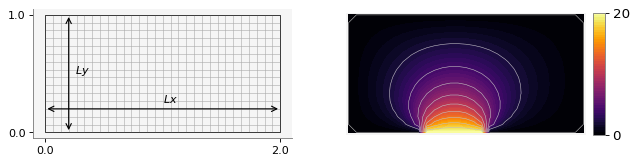
\includegraphics{03_precios_graficas_storytelling_files/figure-pdf/cell-10-output-1.png}

\begin{Shaded}
\begin{Highlighting}[]
\CommentTok{\# Visualización 11: marcamos el rango de precios de introducción}
\NormalTok{fig }\OperatorTok{=}\NormalTok{ plt.figure() }\CommentTok{\# Se define una figura}
\NormalTok{ax }\OperatorTok{=}\NormalTok{ fig.gca()     }\CommentTok{\# Se obtienen los ejes de la figura}

\CommentTok{\# Producto A}
\NormalTok{ax.plot(x2, A, lw}\OperatorTok{=}\DecValTok{3}\NormalTok{, c}\OperatorTok{=}\StringTok{\textquotesingle{}darkgray\textquotesingle{}}\NormalTok{)}
\NormalTok{ax.scatter(x2[}\OperatorTok{{-}}\DecValTok{1}\NormalTok{], A[}\OperatorTok{{-}}\DecValTok{1}\NormalTok{], marker}\OperatorTok{=}\StringTok{\textquotesingle{}o\textquotesingle{}}\NormalTok{, alpha}\OperatorTok{=}\FloatTok{0.85}\NormalTok{, ec }\OperatorTok{=} \StringTok{\textquotesingle{}k\textquotesingle{}}\NormalTok{, s}\OperatorTok{=}\DecValTok{75}\NormalTok{, zorder}\OperatorTok{=}\DecValTok{5}\NormalTok{, color}\OperatorTok{=}\StringTok{\textquotesingle{}forestgreen\textquotesingle{}}\NormalTok{)}

\CommentTok{\# Producto B}
\NormalTok{ax.plot(x2, B, lw}\OperatorTok{=}\DecValTok{3}\NormalTok{, c}\OperatorTok{=}\StringTok{\textquotesingle{}darkgray\textquotesingle{}}\NormalTok{)}
\NormalTok{ax.scatter(x2[}\OperatorTok{{-}}\DecValTok{1}\NormalTok{], B[}\OperatorTok{{-}}\DecValTok{1}\NormalTok{], marker}\OperatorTok{=}\StringTok{\textquotesingle{}o\textquotesingle{}}\NormalTok{, alpha}\OperatorTok{=}\FloatTok{0.85}\NormalTok{, ec }\OperatorTok{=} \StringTok{\textquotesingle{}k\textquotesingle{}}\NormalTok{, s}\OperatorTok{=}\DecValTok{75}\NormalTok{, zorder}\OperatorTok{=}\DecValTok{5}\NormalTok{, color}\OperatorTok{=}\StringTok{\textquotesingle{}forestgreen\textquotesingle{}}\NormalTok{)}

\CommentTok{\# Producto C}
\NormalTok{ax.plot(x2, C, lw}\OperatorTok{=}\DecValTok{3}\NormalTok{, c}\OperatorTok{=}\StringTok{\textquotesingle{}darkgray\textquotesingle{}}\NormalTok{)}
\NormalTok{ax.scatter(x2[}\OperatorTok{{-}}\DecValTok{1}\NormalTok{], C[}\OperatorTok{{-}}\DecValTok{1}\NormalTok{], marker}\OperatorTok{=}\StringTok{\textquotesingle{}o\textquotesingle{}}\NormalTok{, alpha}\OperatorTok{=}\FloatTok{0.85}\NormalTok{, ec }\OperatorTok{=} \StringTok{\textquotesingle{}k\textquotesingle{}}\NormalTok{, s}\OperatorTok{=}\DecValTok{75}\NormalTok{, zorder}\OperatorTok{=}\DecValTok{5}\NormalTok{, color}\OperatorTok{=}\StringTok{\textquotesingle{}forestgreen\textquotesingle{}}\NormalTok{)}

\CommentTok{\# Producto D}
\NormalTok{ax.plot(x2, D, lw}\OperatorTok{=}\DecValTok{3}\NormalTok{, c}\OperatorTok{=}\StringTok{\textquotesingle{}darkgray\textquotesingle{}}\NormalTok{)}
\NormalTok{ax.scatter(x2[}\OperatorTok{{-}}\DecValTok{1}\NormalTok{], D[}\OperatorTok{{-}}\DecValTok{1}\NormalTok{], marker}\OperatorTok{=}\StringTok{\textquotesingle{}o\textquotesingle{}}\NormalTok{, alpha}\OperatorTok{=}\FloatTok{0.85}\NormalTok{, ec }\OperatorTok{=} \StringTok{\textquotesingle{}k\textquotesingle{}}\NormalTok{, s}\OperatorTok{=}\DecValTok{75}\NormalTok{, zorder}\OperatorTok{=}\DecValTok{5}\NormalTok{, color}\OperatorTok{=}\StringTok{\textquotesingle{}forestgreen\textquotesingle{}}\NormalTok{)}

\CommentTok{\# Producto E}
\NormalTok{ax.plot(x2, E, lw}\OperatorTok{=}\DecValTok{3}\NormalTok{, c}\OperatorTok{=}\StringTok{\textquotesingle{}darkgray\textquotesingle{}}\NormalTok{)}
\NormalTok{ax.scatter(x2[}\OperatorTok{{-}}\DecValTok{1}\NormalTok{], E[}\OperatorTok{{-}}\DecValTok{1}\NormalTok{], marker}\OperatorTok{=}\StringTok{\textquotesingle{}o\textquotesingle{}}\NormalTok{, alpha}\OperatorTok{=}\FloatTok{0.85}\NormalTok{, ec }\OperatorTok{=} \StringTok{\textquotesingle{}k\textquotesingle{}}\NormalTok{, s}\OperatorTok{=}\DecValTok{75}\NormalTok{, zorder}\OperatorTok{=}\DecValTok{5}\NormalTok{, color}\OperatorTok{=}\StringTok{\textquotesingle{}forestgreen\textquotesingle{}}\NormalTok{)}

\CommentTok{\# Promedio final}
\NormalTok{precios\_finales }\OperatorTok{=}\NormalTok{ np.array([A[}\OperatorTok{{-}}\DecValTok{1}\NormalTok{], B[}\OperatorTok{{-}}\DecValTok{1}\NormalTok{], C[}\OperatorTok{{-}}\DecValTok{1}\NormalTok{], D[}\OperatorTok{{-}}\DecValTok{1}\NormalTok{], E[}\OperatorTok{{-}}\DecValTok{1}\NormalTok{],])}
\NormalTok{promedio\_final }\OperatorTok{=}\NormalTok{ np.mean(precios\_finales)}
\NormalTok{ax.scatter(x2[}\OperatorTok{{-}}\DecValTok{1}\NormalTok{], promedio\_final, marker}\OperatorTok{=}\StringTok{\textquotesingle{}\textless{}\textquotesingle{}}\NormalTok{, alpha}\OperatorTok{=}\FloatTok{0.85}\NormalTok{, ec }\OperatorTok{=} \StringTok{\textquotesingle{}k\textquotesingle{}}\NormalTok{, s}\OperatorTok{=}\DecValTok{75}\NormalTok{, }
\NormalTok{           zorder}\OperatorTok{=}\DecValTok{5}\NormalTok{, color}\OperatorTok{=}\StringTok{\textquotesingle{}orange\textquotesingle{}}\NormalTok{, label}\OperatorTok{=}\StringTok{\textquotesingle{}Promedio\textquotesingle{}}\NormalTok{)}

\CommentTok{\# Límites en los ejes}
\NormalTok{ax.set\_ylim(}\DecValTok{0}\NormalTok{,}\DecValTok{500}\NormalTok{)}
\NormalTok{ax.set\_xlim(}\FloatTok{2012.5}\NormalTok{,}\FloatTok{2019.5}\NormalTok{)}

\CommentTok{\# Marcas sobre los ejes}
\NormalTok{ax.set\_xticks(ticks}\OperatorTok{=}\NormalTok{[i }\ControlFlowTok{for}\NormalTok{ i }\KeywordTok{in} \BuiltInTok{range}\NormalTok{(}\DecValTok{2013}\NormalTok{,}\DecValTok{2020}\NormalTok{)])}
\NormalTok{ax.set\_yticks(ticks}\OperatorTok{=}\NormalTok{[}\DecValTok{0}\NormalTok{,}\DecValTok{100}\NormalTok{,}\DecValTok{200}\NormalTok{,}\DecValTok{300}\NormalTok{,}\DecValTok{400}\NormalTok{,}\DecValTok{500}\NormalTok{], }
\NormalTok{              labels}\OperatorTok{=}\NormalTok{[}\StringTok{\textquotesingle{}\textbackslash{}$0\textquotesingle{}}\NormalTok{,}\StringTok{\textquotesingle{}\textbackslash{}$100\textquotesingle{}}\NormalTok{,}\StringTok{\textquotesingle{}\textbackslash{}$200\textquotesingle{}}\NormalTok{,}\StringTok{\textquotesingle{}\textbackslash{}$300\textquotesingle{}}\NormalTok{,}\StringTok{\textquotesingle{}\textbackslash{}$400\textquotesingle{}}\NormalTok{,}\StringTok{\textquotesingle{}\textbackslash{}$500\textquotesingle{}}\NormalTok{])}

\CommentTok{\# Rejilla}
\NormalTok{ax.grid()}

\NormalTok{ax.text(x }\OperatorTok{=}\NormalTok{ x2[}\DecValTok{0}\NormalTok{]}\OperatorTok{{-}}\FloatTok{0.20}\NormalTok{, y }\OperatorTok{=}\NormalTok{ A[}\DecValTok{0}\NormalTok{], s }\OperatorTok{=} \StringTok{\textquotesingle{}A\textquotesingle{}}\NormalTok{, fontsize }\OperatorTok{=} \DecValTok{18}\NormalTok{)}
\NormalTok{ax.text(x }\OperatorTok{=}\NormalTok{ x2[}\DecValTok{0}\NormalTok{]}\OperatorTok{{-}}\FloatTok{0.20}\NormalTok{, y }\OperatorTok{=}\NormalTok{ B[}\DecValTok{0}\NormalTok{]}\OperatorTok{{-}}\DecValTok{20}\NormalTok{, s }\OperatorTok{=} \StringTok{\textquotesingle{}B\textquotesingle{}}\NormalTok{, fontsize }\OperatorTok{=} \DecValTok{18}\NormalTok{)}
\NormalTok{ax.text(x }\OperatorTok{=}\NormalTok{ x2[}\DecValTok{2}\NormalTok{]}\OperatorTok{{-}}\FloatTok{0.20}\NormalTok{, y }\OperatorTok{=}\NormalTok{ C[}\DecValTok{2}\NormalTok{]}\OperatorTok{{-}}\DecValTok{20}\NormalTok{, s }\OperatorTok{=} \StringTok{\textquotesingle{}C\textquotesingle{}}\NormalTok{, fontsize }\OperatorTok{=} \DecValTok{18}\NormalTok{)}
\NormalTok{ax.text(x }\OperatorTok{=}\NormalTok{ x2[}\DecValTok{3}\NormalTok{]}\OperatorTok{{-}}\FloatTok{0.20}\NormalTok{, y }\OperatorTok{=}\NormalTok{ D[}\DecValTok{3}\NormalTok{]}\OperatorTok{{-}}\DecValTok{20}\NormalTok{, s }\OperatorTok{=} \StringTok{\textquotesingle{}D\textquotesingle{}}\NormalTok{, fontsize }\OperatorTok{=} \DecValTok{18}\NormalTok{)}
\NormalTok{ax.text(x }\OperatorTok{=}\NormalTok{ x2[}\DecValTok{5}\NormalTok{]}\OperatorTok{{-}}\FloatTok{0.20}\NormalTok{, y }\OperatorTok{=}\NormalTok{ E[}\DecValTok{5}\NormalTok{]}\OperatorTok{{-}}\DecValTok{20}\NormalTok{, s }\OperatorTok{=} \StringTok{\textquotesingle{}E\textquotesingle{}}\NormalTok{, fontsize }\OperatorTok{=} \DecValTok{18}\NormalTok{)}

\NormalTok{ax.spines[}\StringTok{\textquotesingle{}right\textquotesingle{}}\NormalTok{].set\_visible(}\VariableTok{False}\NormalTok{)}
\NormalTok{ax.spines[}\StringTok{\textquotesingle{}top\textquotesingle{}}\NormalTok{].set\_visible(}\VariableTok{False}\NormalTok{)}
\NormalTok{ax.spines[}\StringTok{\textquotesingle{}left\textquotesingle{}}\NormalTok{].set\_color(}\StringTok{\textquotesingle{}gray\textquotesingle{}}\NormalTok{)}
\NormalTok{ax.spines[}\StringTok{\textquotesingle{}bottom\textquotesingle{}}\NormalTok{].set\_color(}\StringTok{\textquotesingle{}gray\textquotesingle{}}\NormalTok{)}
\NormalTok{ax.tick\_params(axis}\OperatorTok{=}\StringTok{\textquotesingle{}x\textquotesingle{}}\NormalTok{, colors}\OperatorTok{=}\StringTok{\textquotesingle{}\#444444\textquotesingle{}}\NormalTok{)}
\NormalTok{ax.tick\_params(axis}\OperatorTok{=}\StringTok{\textquotesingle{}y\textquotesingle{}}\NormalTok{, colors}\OperatorTok{=}\StringTok{\textquotesingle{}\#444444\textquotesingle{}}\NormalTok{)}

\NormalTok{plt.suptitle(}\StringTok{\textquotesingle{}Precio promedio por año\textquotesingle{}}\NormalTok{, fontsize}\OperatorTok{=}\DecValTok{24}\NormalTok{, x }\OperatorTok{=}\FloatTok{0.275}\NormalTok{, y}\OperatorTok{=}\FloatTok{1.05}\NormalTok{)}
\NormalTok{plt.legend(loc}\OperatorTok{=}\StringTok{\textquotesingle{}lower right\textquotesingle{}}\NormalTok{)}
\NormalTok{plt.savefig(}\StringTok{\textquotesingle{}vis6.png\textquotesingle{}}\NormalTok{,bbox\_inches}\OperatorTok{=}\StringTok{\textquotesingle{}tight\textquotesingle{}}\NormalTok{, dpi}\OperatorTok{=}\DecValTok{150}\NormalTok{)}
\NormalTok{plt.show()}
\end{Highlighting}
\end{Shaded}

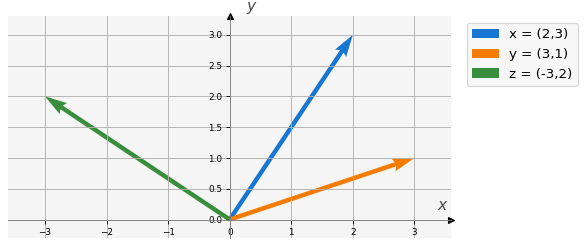
\includegraphics{03_precios_graficas_storytelling_files/figure-pdf/cell-11-output-1.png}

\begin{Shaded}
\begin{Highlighting}[]
\CommentTok{\# Visualización 11: marcamos el rango de precios de introducción}
\NormalTok{fig }\OperatorTok{=}\NormalTok{ plt.figure() }\CommentTok{\# Se define una figura}
\NormalTok{ax }\OperatorTok{=}\NormalTok{ fig.gca()     }\CommentTok{\# Se obtienen los ejes de la figura}

\CommentTok{\# Producto A}
\NormalTok{ax.plot(x2, A, lw}\OperatorTok{=}\DecValTok{3}\NormalTok{, c}\OperatorTok{=}\StringTok{\textquotesingle{}darkgray\textquotesingle{}}\NormalTok{)}
\NormalTok{ax.scatter(x2[}\OperatorTok{{-}}\DecValTok{1}\NormalTok{], A[}\OperatorTok{{-}}\DecValTok{1}\NormalTok{], marker}\OperatorTok{=}\StringTok{\textquotesingle{}o\textquotesingle{}}\NormalTok{, alpha}\OperatorTok{=}\FloatTok{0.85}\NormalTok{, ec }\OperatorTok{=} \StringTok{\textquotesingle{}k\textquotesingle{}}\NormalTok{, s}\OperatorTok{=}\DecValTok{75}\NormalTok{, zorder}\OperatorTok{=}\DecValTok{5}\NormalTok{, color}\OperatorTok{=}\StringTok{\textquotesingle{}forestgreen\textquotesingle{}}\NormalTok{)}

\CommentTok{\# Producto B}
\NormalTok{ax.plot(x2, B, lw}\OperatorTok{=}\DecValTok{3}\NormalTok{, c}\OperatorTok{=}\StringTok{\textquotesingle{}darkgray\textquotesingle{}}\NormalTok{)}
\NormalTok{ax.scatter(x2[}\OperatorTok{{-}}\DecValTok{1}\NormalTok{], B[}\OperatorTok{{-}}\DecValTok{1}\NormalTok{], marker}\OperatorTok{=}\StringTok{\textquotesingle{}o\textquotesingle{}}\NormalTok{, alpha}\OperatorTok{=}\FloatTok{0.85}\NormalTok{, ec }\OperatorTok{=} \StringTok{\textquotesingle{}k\textquotesingle{}}\NormalTok{, s}\OperatorTok{=}\DecValTok{75}\NormalTok{, zorder}\OperatorTok{=}\DecValTok{5}\NormalTok{, color}\OperatorTok{=}\StringTok{\textquotesingle{}forestgreen\textquotesingle{}}\NormalTok{)}

\CommentTok{\# Producto C}
\NormalTok{ax.plot(x2, C, lw}\OperatorTok{=}\DecValTok{3}\NormalTok{, c}\OperatorTok{=}\StringTok{\textquotesingle{}darkgray\textquotesingle{}}\NormalTok{)}
\NormalTok{ax.scatter(x2[}\OperatorTok{{-}}\DecValTok{1}\NormalTok{], C[}\OperatorTok{{-}}\DecValTok{1}\NormalTok{], marker}\OperatorTok{=}\StringTok{\textquotesingle{}o\textquotesingle{}}\NormalTok{, alpha}\OperatorTok{=}\FloatTok{0.85}\NormalTok{, ec }\OperatorTok{=} \StringTok{\textquotesingle{}k\textquotesingle{}}\NormalTok{, s}\OperatorTok{=}\DecValTok{75}\NormalTok{, zorder}\OperatorTok{=}\DecValTok{5}\NormalTok{, color}\OperatorTok{=}\StringTok{\textquotesingle{}forestgreen\textquotesingle{}}\NormalTok{)}

\CommentTok{\# Producto D}
\NormalTok{ax.plot(x2, D, lw}\OperatorTok{=}\DecValTok{3}\NormalTok{, c}\OperatorTok{=}\StringTok{\textquotesingle{}darkgray\textquotesingle{}}\NormalTok{)}
\NormalTok{ax.scatter(x2[}\OperatorTok{{-}}\DecValTok{1}\NormalTok{], D[}\OperatorTok{{-}}\DecValTok{1}\NormalTok{], marker}\OperatorTok{=}\StringTok{\textquotesingle{}o\textquotesingle{}}\NormalTok{, alpha}\OperatorTok{=}\FloatTok{0.85}\NormalTok{, ec }\OperatorTok{=} \StringTok{\textquotesingle{}k\textquotesingle{}}\NormalTok{, s}\OperatorTok{=}\DecValTok{75}\NormalTok{, zorder}\OperatorTok{=}\DecValTok{5}\NormalTok{, color}\OperatorTok{=}\StringTok{\textquotesingle{}forestgreen\textquotesingle{}}\NormalTok{)}

\CommentTok{\# Producto E}
\NormalTok{ax.plot(x2, E, lw}\OperatorTok{=}\DecValTok{3}\NormalTok{, c}\OperatorTok{=}\StringTok{\textquotesingle{}darkgray\textquotesingle{}}\NormalTok{)}
\NormalTok{ax.scatter(x2[}\OperatorTok{{-}}\DecValTok{1}\NormalTok{], E[}\OperatorTok{{-}}\DecValTok{1}\NormalTok{], marker}\OperatorTok{=}\StringTok{\textquotesingle{}o\textquotesingle{}}\NormalTok{, alpha}\OperatorTok{=}\FloatTok{0.85}\NormalTok{, ec }\OperatorTok{=} \StringTok{\textquotesingle{}k\textquotesingle{}}\NormalTok{, s}\OperatorTok{=}\DecValTok{75}\NormalTok{, zorder}\OperatorTok{=}\DecValTok{5}\NormalTok{, color}\OperatorTok{=}\StringTok{\textquotesingle{}forestgreen\textquotesingle{}}\NormalTok{)}

\CommentTok{\# Promedio final}
\NormalTok{precios\_finales }\OperatorTok{=}\NormalTok{ np.array([A[}\OperatorTok{{-}}\DecValTok{1}\NormalTok{], B[}\OperatorTok{{-}}\DecValTok{1}\NormalTok{], C[}\OperatorTok{{-}}\DecValTok{1}\NormalTok{], D[}\OperatorTok{{-}}\DecValTok{1}\NormalTok{], E[}\OperatorTok{{-}}\DecValTok{1}\NormalTok{],])}
\NormalTok{promedio\_final }\OperatorTok{=}\NormalTok{ np.mean(precios\_finales)}
\NormalTok{ax.scatter(x2[}\OperatorTok{{-}}\DecValTok{1}\NormalTok{], promedio\_final, marker}\OperatorTok{=}\StringTok{\textquotesingle{}\textless{}\textquotesingle{}}\NormalTok{, alpha}\OperatorTok{=}\FloatTok{0.85}\NormalTok{, ec }\OperatorTok{=} \StringTok{\textquotesingle{}k\textquotesingle{}}\NormalTok{, s}\OperatorTok{=}\DecValTok{75}\NormalTok{, }
\NormalTok{           zorder}\OperatorTok{=}\DecValTok{5}\NormalTok{, color}\OperatorTok{=}\StringTok{\textquotesingle{}orange\textquotesingle{}}\NormalTok{, label}\OperatorTok{=}\StringTok{\textquotesingle{}Promedio\textquotesingle{}}\NormalTok{)}

\CommentTok{\# Límites en los ejes}
\NormalTok{ax.set\_ylim(}\DecValTok{0}\NormalTok{,}\DecValTok{500}\NormalTok{)}
\NormalTok{ax.set\_xlim(}\FloatTok{2012.5}\NormalTok{,}\FloatTok{2019.5}\NormalTok{)}

\CommentTok{\# Marcas sobre los ejes}
\NormalTok{ax.set\_xticks(ticks}\OperatorTok{=}\NormalTok{[i }\ControlFlowTok{for}\NormalTok{ i }\KeywordTok{in} \BuiltInTok{range}\NormalTok{(}\DecValTok{2013}\NormalTok{,}\DecValTok{2020}\NormalTok{)])}
\NormalTok{ax.set\_yticks(ticks}\OperatorTok{=}\NormalTok{[}\DecValTok{0}\NormalTok{,}\DecValTok{100}\NormalTok{,}\DecValTok{200}\NormalTok{,}\DecValTok{300}\NormalTok{,}\DecValTok{400}\NormalTok{,}\DecValTok{500}\NormalTok{], }
\NormalTok{              labels}\OperatorTok{=}\NormalTok{[}\StringTok{\textquotesingle{}\textbackslash{}$0\textquotesingle{}}\NormalTok{,}\StringTok{\textquotesingle{}\textbackslash{}$100\textquotesingle{}}\NormalTok{,}\StringTok{\textquotesingle{}\textbackslash{}$200\textquotesingle{}}\NormalTok{,}\StringTok{\textquotesingle{}\textbackslash{}$300\textquotesingle{}}\NormalTok{,}\StringTok{\textquotesingle{}\textbackslash{}$400\textquotesingle{}}\NormalTok{,}\StringTok{\textquotesingle{}\textbackslash{}$500\textquotesingle{}}\NormalTok{])}

\CommentTok{\# Rejilla}
\NormalTok{ax.grid()}

\CommentTok{\# Etiquetado de cada línea}
\NormalTok{ax.text(x }\OperatorTok{=}\NormalTok{ x2[}\DecValTok{0}\NormalTok{]}\OperatorTok{{-}}\FloatTok{0.20}\NormalTok{, y }\OperatorTok{=}\NormalTok{ A[}\DecValTok{0}\NormalTok{], s }\OperatorTok{=} \StringTok{\textquotesingle{}A\textquotesingle{}}\NormalTok{, fontsize }\OperatorTok{=} \DecValTok{18}\NormalTok{)}
\NormalTok{ax.text(x }\OperatorTok{=}\NormalTok{ x2[}\DecValTok{0}\NormalTok{]}\OperatorTok{{-}}\FloatTok{0.20}\NormalTok{, y }\OperatorTok{=}\NormalTok{ B[}\DecValTok{0}\NormalTok{]}\OperatorTok{{-}}\DecValTok{20}\NormalTok{, s }\OperatorTok{=} \StringTok{\textquotesingle{}B\textquotesingle{}}\NormalTok{, fontsize }\OperatorTok{=} \DecValTok{18}\NormalTok{)}
\NormalTok{ax.text(x }\OperatorTok{=}\NormalTok{ x2[}\DecValTok{2}\NormalTok{]}\OperatorTok{{-}}\FloatTok{0.20}\NormalTok{, y }\OperatorTok{=}\NormalTok{ C[}\DecValTok{2}\NormalTok{]}\OperatorTok{{-}}\DecValTok{20}\NormalTok{, s }\OperatorTok{=} \StringTok{\textquotesingle{}C\textquotesingle{}}\NormalTok{, fontsize }\OperatorTok{=} \DecValTok{18}\NormalTok{)}
\NormalTok{ax.text(x }\OperatorTok{=}\NormalTok{ x2[}\DecValTok{3}\NormalTok{]}\OperatorTok{{-}}\FloatTok{0.20}\NormalTok{, y }\OperatorTok{=}\NormalTok{ D[}\DecValTok{3}\NormalTok{]}\OperatorTok{{-}}\DecValTok{20}\NormalTok{, s }\OperatorTok{=} \StringTok{\textquotesingle{}D\textquotesingle{}}\NormalTok{, fontsize }\OperatorTok{=} \DecValTok{18}\NormalTok{)}
\NormalTok{ax.text(x }\OperatorTok{=}\NormalTok{ x2[}\DecValTok{5}\NormalTok{]}\OperatorTok{{-}}\FloatTok{0.20}\NormalTok{, y }\OperatorTok{=}\NormalTok{ E[}\DecValTok{5}\NormalTok{]}\OperatorTok{{-}}\DecValTok{20}\NormalTok{, s }\OperatorTok{=} \StringTok{\textquotesingle{}E\textquotesingle{}}\NormalTok{, fontsize }\OperatorTok{=} \DecValTok{18}\NormalTok{)}

\CommentTok{\# Eliminación de algunas líneas del recuadro}
\NormalTok{ax.spines[}\StringTok{\textquotesingle{}right\textquotesingle{}}\NormalTok{].set\_visible(}\VariableTok{False}\NormalTok{)}
\NormalTok{ax.spines[}\StringTok{\textquotesingle{}top\textquotesingle{}}\NormalTok{].set\_visible(}\VariableTok{False}\NormalTok{)}
\NormalTok{ax.spines[}\StringTok{\textquotesingle{}left\textquotesingle{}}\NormalTok{].set\_color(}\StringTok{\textquotesingle{}gray\textquotesingle{}}\NormalTok{)}
\NormalTok{ax.spines[}\StringTok{\textquotesingle{}bottom\textquotesingle{}}\NormalTok{].set\_color(}\StringTok{\textquotesingle{}gray\textquotesingle{}}\NormalTok{)}

\CommentTok{\# Color de los ticks}
\NormalTok{ax.tick\_params(axis}\OperatorTok{=}\StringTok{\textquotesingle{}x\textquotesingle{}}\NormalTok{, colors}\OperatorTok{=}\StringTok{\textquotesingle{}\#444444\textquotesingle{}}\NormalTok{)}
\NormalTok{ax.tick\_params(axis}\OperatorTok{=}\StringTok{\textquotesingle{}y\textquotesingle{}}\NormalTok{, colors}\OperatorTok{=}\StringTok{\textquotesingle{}\#444444\textquotesingle{}}\NormalTok{)}

\CommentTok{\# Recuadro para indicar la región del precio final}
\NormalTok{left, bottom, width, height }\OperatorTok{=}\NormalTok{ (}\DecValTok{2012}\NormalTok{, }\DecValTok{150}\NormalTok{, }\DecValTok{8}\NormalTok{, }\DecValTok{50}\NormalTok{)}
\NormalTok{rect }\OperatorTok{=}\NormalTok{ plt.Rectangle((left, bottom), width, height,}
\NormalTok{                     facecolor}\OperatorTok{=}\StringTok{"black"}\NormalTok{, alpha}\OperatorTok{=}\FloatTok{0.1}\NormalTok{)}
\NormalTok{ax.add\_patch(rect)}
\NormalTok{ax.text(x }\OperatorTok{=}\NormalTok{ x2[}\DecValTok{0}\NormalTok{]}\OperatorTok{{-}}\FloatTok{0.25}\NormalTok{, y }\OperatorTok{=} \DecValTok{165}\NormalTok{, s }\OperatorTok{=} \StringTok{\textquotesingle{}Rango de precios de introducción\textquotesingle{}}\NormalTok{, fontsize }\OperatorTok{=} \DecValTok{12}\NormalTok{, color}\OperatorTok{=}\StringTok{\textquotesingle{}navy\textquotesingle{}}\NormalTok{)}

\NormalTok{plt.suptitle(}\StringTok{\textquotesingle{}Precio promedio por año\textquotesingle{}}\NormalTok{, fontsize}\OperatorTok{=}\DecValTok{24}\NormalTok{, x }\OperatorTok{=}\FloatTok{0.275}\NormalTok{, y}\OperatorTok{=}\FloatTok{1.05}\NormalTok{)}
\NormalTok{plt.legend(loc}\OperatorTok{=}\StringTok{\textquotesingle{}lower right\textquotesingle{}}\NormalTok{)}
\NormalTok{plt.savefig(}\StringTok{\textquotesingle{}vis\_final.png\textquotesingle{}}\NormalTok{,bbox\_inches}\OperatorTok{=}\StringTok{\textquotesingle{}tight\textquotesingle{}}\NormalTok{, dpi}\OperatorTok{=}\DecValTok{150}\NormalTok{)}
\NormalTok{plt.show()}
\end{Highlighting}
\end{Shaded}

\includegraphics{03_precios_graficas_storytelling_files/figure-pdf/cell-12-output-1.png}

\bookmarksetup{startatroot}

\chapter{Análisis de la tasa de fertilidad total
mundial}\label{anuxe1lisis-de-la-tasa-de-fertilidad-total-mundial}

This notebook by Luis M. de la Cruz Salas is licensed under
Attribution-NonCommercial-NoDerivatives 4.0 International

Para lograr una excelente visualización de datos se debe tener:
\textbf{mucha curiosidad} e interés en \textbf{muchos temas variados}
que pueden parecer poco relacionados entre ellos: matemáticas,
demografía, epidemiología, economía, deportes, ventas por internet,
historia, psicología y muchos etcéteras.

Durante el proceso de esta visualización la vida tenderá a convertirse
en un \textbf{caos intelectual}, pero \textbf{sistemático y
emocionante}.

La \textbf{visualización de datos} es muy importante, pues es posible
que sea \textbf{lo único que vean tus interlocutores}: cliente, colega,
jefe, tutor, jurado, lectores de un periódico, público en una
conferencia, \ldots{} y probablemente a ellos no les interese mucho los
datos numéricos o los algoritmos usados en su análisis.

El público a quien deseas transmitir tus hallazgos olvidarán muy pronto
los numéros; pero si introduces tus hallazgos mediante un relato que
cuente la historia de los datos, es posible que ellos se lleven un buen
sabor de boca y recuerden la información recibida por mucho más tiempo e
incluso tomen acciones.

\section{Objetivo}\label{objetivo}

\begin{itemize}
\item
  Obtener información de http://data.un.org/ de las siguientes
  variables:

  \begin{itemize}
  \tightlist
  \item
    Tasa de fertilidad total (TFR)
  \item
    Ingreso per cápita (GDP)
  \item
    Nivel de educación (EDU)
  \item
    Esperanza de vida al nacer (LEB)
  \end{itemize}
\item
  Construir una visualización que permita comparar el cambio en el Total
  Fertility Rate (TFR) en función del tiempo para varias países.
\item
  Generar un data set para el índice de desarrollo humano (HDI) de
  acuerdo con: https://en.wikipedia.org/wiki/Human\_Development\_Index
\end{itemize}

HeCompA - Anscombe by Luis M. de la Cruz is licensed under
Attribution-ShareAlike 4.0 International

\textbf{Trabajo realizado con el apoyo del Programa UNAM-DGAPA-PAPIME
PE101922}

\begin{Shaded}
\begin{Highlighting}[]
\ImportTok{import}\NormalTok{ numpy }\ImportTok{as}\NormalTok{ np}
\ImportTok{import}\NormalTok{ matplotlib.pyplot }\ImportTok{as}\NormalTok{ plt}
\ImportTok{import}\NormalTok{ pandas }\ImportTok{as}\NormalTok{ pd }
\ImportTok{from}\NormalTok{ math }\ImportTok{import}\NormalTok{ ceil}

\CommentTok{\# Esta biblioteca solo funciona en la plataforma www.macti.unam.mx}
\CommentTok{\# Si no estas en esa plataforma, solo comenta la línea que sigue.}
\ImportTok{import}\NormalTok{ macti.visual}
\end{Highlighting}
\end{Shaded}

\bookmarksetup{startatroot}

\chapter{Conjuntos de datos.}\label{conjuntos-de-datos.}

Los datos ya están en el directorio de esta notebook. Solo los leemos.

\begin{Shaded}
\begin{Highlighting}[]
\NormalTok{TFR }\OperatorTok{=}\NormalTok{ pd.read\_csv(}\StringTok{\textquotesingle{}UNdata\_Export\_20230621\_205538168.zip\textquotesingle{}}\NormalTok{)}
\CommentTok{\# GPD per capita}
\NormalTok{GDP }\OperatorTok{=}\NormalTok{ pd.read\_csv(}\StringTok{\textquotesingle{}UNdata\_Export\_20230624\_011417717.zip\textquotesingle{}}\NormalTok{)}
\CommentTok{\# Life expectancy at birth }
\NormalTok{LEB }\OperatorTok{=}\NormalTok{ pd.read\_csv(}\StringTok{\textquotesingle{}UNdata\_Export\_20230624\_013747471.zip\textquotesingle{}}\NormalTok{)}
\CommentTok{\# Gross enrolment ratio. Tertiary education}
\NormalTok{EDU }\OperatorTok{=}\NormalTok{ pd.read\_csv(}\StringTok{\textquotesingle{}UNdata\_Export\_20230624\_014454110.zip\textquotesingle{}}\NormalTok{)}
\end{Highlighting}
\end{Shaded}

\begin{Shaded}
\begin{Highlighting}[]
\NormalTok{EDU.head()}
\end{Highlighting}
\end{Shaded}

\begin{longtable}[]{@{}lllllll@{}}
\toprule\noalign{}
& Reference Area & Time Period & Sex & Age group & Units of measurement
& Observation Value \\
\midrule\noalign{}
\endhead
\bottomrule\noalign{}
\endlastfoot
0 & Afghanistan & 2014 & Female & Not applicable & Percent & 3.67329 \\
1 & Afghanistan & 2014 & Male & Not applicable & Percent & 13.28657 \\
2 & Afghanistan & 2014 & All genders & Not applicable & Percent &
8.66280 \\
3 & Afghanistan & 2011 & Female & Not applicable & Percent & 1.89233 \\
4 & Afghanistan & 2011 & All genders & Not applicable & Percent &
3.75598 \\
\end{longtable}

\begin{Shaded}
\begin{Highlighting}[]
\BuiltInTok{print}\NormalTok{(TFR.columns)}
\BuiltInTok{print}\NormalTok{(GDP.columns)}
\BuiltInTok{print}\NormalTok{(LEB.columns)}
\BuiltInTok{print}\NormalTok{(EDU.columns)}
\end{Highlighting}
\end{Shaded}

\begin{verbatim}
Index(['Country or Area', 'Year(s)', 'Variant', 'Value'], dtype='object')
Index(['Country or Area', 'Year', 'Item', 'Value'], dtype='object')
Index(['Country or Area', 'Year(s)', 'Variant', 'Value'], dtype='object')
Index(['Reference Area', 'Time Period', 'Sex', 'Age group',
       'Units of measurement', 'Observation Value'],
      dtype='object')
\end{verbatim}

Agrupamos los datos por países y regiones geográficas.

\begin{Shaded}
\begin{Highlighting}[]
\NormalTok{TFR\_group }\OperatorTok{=}\NormalTok{ TFR.groupby(}\StringTok{\textquotesingle{}Country or Area\textquotesingle{}}\NormalTok{)}
\NormalTok{GDP\_group }\OperatorTok{=}\NormalTok{ GDP.groupby(}\StringTok{\textquotesingle{}Country or Area\textquotesingle{}}\NormalTok{)}
\NormalTok{LEB\_group }\OperatorTok{=}\NormalTok{ LEB.groupby(}\StringTok{\textquotesingle{}Country or Area\textquotesingle{}}\NormalTok{)}
\NormalTok{EDU\_group }\OperatorTok{=}\NormalTok{ EDU.groupby(}\StringTok{\textquotesingle{}Reference Area\textquotesingle{}}\NormalTok{)}
\end{Highlighting}
\end{Shaded}

Determinamos los países que se tienen en cada conjunto de datos

\begin{Shaded}
\begin{Highlighting}[]
\NormalTok{TFR\_countries }\OperatorTok{=}\NormalTok{ TFR\_group.groups.keys()}
\NormalTok{GDP\_countries }\OperatorTok{=}\NormalTok{ GDP\_group.groups.keys()}
\NormalTok{LEB\_countries }\OperatorTok{=}\NormalTok{ LEB\_group.groups.keys()}
\NormalTok{EDU\_countries }\OperatorTok{=}\NormalTok{ EDU\_group.groups.keys()}
\end{Highlighting}
\end{Shaded}

\begin{Shaded}
\begin{Highlighting}[]
\BuiltInTok{print}\NormalTok{(}\BuiltInTok{len}\NormalTok{(TFR\_countries))}
\BuiltInTok{print}\NormalTok{(}\BuiltInTok{len}\NormalTok{(GDP\_countries))}
\BuiltInTok{print}\NormalTok{(}\BuiltInTok{len}\NormalTok{(LEB\_countries))}
\BuiltInTok{print}\NormalTok{(}\BuiltInTok{len}\NormalTok{(EDU\_countries))}
\end{Highlighting}
\end{Shaded}

\begin{verbatim}
284
220
284
220
\end{verbatim}

\begin{Shaded}
\begin{Highlighting}[]
\BuiltInTok{print}\NormalTok{(TFR\_countries)}
\end{Highlighting}
\end{Shaded}

\begin{verbatim}
dict_keys(['Afghanistan', 'Africa', 'Albania', 'Algeria', 'American Samoa', 'Andorra', 'Angola', 'Anguilla', 'Antigua and Barbuda', 'Argentina', 'Armenia', 'Aruba', 'Asia', 'Australia', 'Australia/New Zealand', 'Austria', 'Azerbaijan', 'Bahamas', 'Bahrain', 'Bangladesh', 'Barbados', 'Belarus', 'Belgium', 'Belize', 'Benin', 'Bermuda', 'Bhutan', 'Bolivia (Plurinational State of)', 'Bonaire, Sint Eustatius and Saba', 'Bosnia and Herzegovina', 'Botswana', 'Brazil', 'British Virgin Islands', 'Brunei Darussalam', 'Bulgaria', 'Burkina Faso', 'Burundi', 'Cabo Verde', 'Cambodia', 'Cameroon', 'Canada', 'Caribbean', 'Cayman Islands', 'Central African Republic', 'Central America', 'Central Asia', 'Central and Southern Asia', 'Chad', 'Chile', 'China', 'China, Hong Kong SAR', 'China, Macao SAR', 'Colombia', 'Comoros', 'Congo', 'Cook Islands', 'Costa Rica', 'Croatia', 'Cuba', 'Curaçao', 'Cyprus', 'Czechia', "Côte d'Ivoire", "Dem. People's Republic of Korea", 'Democratic Republic of the Congo', 'Denmark', 'Djibouti', 'Dominica', 'Dominican Republic', 'Eastern Africa', 'Eastern Asia', 'Eastern Europe', 'Eastern and South-Eastern Asia', 'Ecuador', 'Egypt', 'El Salvador', 'Equatorial Guinea', 'Eritrea', 'Estonia', 'Eswatini', 'Ethiopia', 'Europe', 'Europe and Northern America', 'Falkland Islands (Malvinas)', 'Faroe Islands', 'Fiji', 'Finland', 'France', 'French Guiana', 'French Polynesia', 'Gabon', 'Gambia', 'Georgia', 'Germany', 'Ghana', 'Gibraltar', 'Greece', 'Greenland', 'Grenada', 'Guadeloupe', 'Guam', 'Guatemala', 'Guernsey', 'Guinea', 'Guinea-Bissau', 'Guyana', 'Haiti', 'High-income countries', 'Holy See', 'Honduras', 'Hungary', 'Iceland', 'India', 'Indonesia', 'Iran (Islamic Republic of)', 'Iraq', 'Ireland', 'Isle of Man', 'Israel', 'Italy', 'Jamaica', 'Japan', 'Jersey', 'Jordan', 'Kazakhstan', 'Kenya', 'Kiribati', 'Kosovo (under UNSC res. 1244)', 'Kuwait', 'Kyrgyzstan', 'Land-locked Developing Countries (LLDC)', "Lao People's Democratic Republic", 'Latin America and the Caribbean', 'Latvia', 'Least developed countries', 'Lebanon', 'Lesotho', 'Less developed regions', 'Less developed regions, excluding China', 'Less developed regions, excluding least developed countries', 'Liberia', 'Libya', 'Liechtenstein', 'Lithuania', 'Low-income countries', 'Lower-middle-income countries', 'Luxembourg', 'Madagascar', 'Malawi', 'Malaysia', 'Maldives', 'Mali', 'Malta', 'Marshall Islands', 'Martinique', 'Mauritania', 'Mauritius', 'Mayotte', 'Melanesia', 'Mexico', 'Micronesia', 'Micronesia (Fed. States of)', 'Middle Africa', 'Middle-income countries', 'Monaco', 'Mongolia', 'Montenegro', 'Montserrat', 'More developed regions', 'Morocco', 'Mozambique', 'Myanmar', 'Namibia', 'Nauru', 'Nepal', 'Netherlands', 'New Caledonia', 'New Zealand', 'Nicaragua', 'Niger', 'Nigeria', 'Niue', 'No income group available', 'North Macedonia', 'Northern Africa', 'Northern Africa and Western Asia', 'Northern America', 'Northern Europe', 'Northern Mariana Islands', 'Norway', 'Oceania', 'Oceania (excluding Australia and New Zealand)', 'Oman', 'Other non-specified areas', 'Pakistan', 'Palau', 'Panama', 'Papua New Guinea', 'Paraguay', 'Peru', 'Philippines', 'Poland', 'Polynesia', 'Portugal', 'Puerto Rico', 'Qatar', 'Republic of Korea', 'Republic of Moldova', 'Romania', 'Russian Federation', 'Rwanda', 'Réunion', 'Saint Barthélemy', 'Saint Helena', 'Saint Kitts and Nevis', 'Saint Lucia', 'Saint Martin (French part)', 'Saint Pierre and Miquelon', 'Saint Vincent and the Grenadines', 'Samoa', 'San Marino', 'Sao Tome and Principe', 'Saudi Arabia', 'Senegal', 'Serbia', 'Seychelles', 'Sierra Leone', 'Singapore', 'Sint Maarten (Dutch part)', 'Slovakia', 'Slovenia', 'Small Island Developing States (SIDS)', 'Solomon Islands', 'Somalia', 'South Africa', 'South America', 'South Sudan', 'South-Eastern Asia', 'Southern Africa', 'Southern Asia', 'Southern Europe', 'Spain', 'Sri Lanka', 'State of Palestine', 'Sub-Saharan Africa', 'Sudan', 'Suriname', 'Sweden', 'Switzerland', 'Syrian Arab Republic', 'Tajikistan', 'Thailand', 'Timor-Leste', 'Togo', 'Tokelau', 'Tonga', 'Trinidad and Tobago', 'Tunisia', 'Turkmenistan', 'Turks and Caicos Islands', 'Tuvalu', 'Türkiye', 'Uganda', 'Ukraine', 'United Arab Emirates', 'United Kingdom', 'United Republic of Tanzania', 'United States Virgin Islands', 'United States of America', 'Upper-middle-income countries', 'Uruguay', 'Uzbekistan', 'Vanuatu', 'Venezuela (Bolivarian Republic of)', 'Viet Nam', 'Wallis and Futuna Islands', 'Western Africa', 'Western Asia', 'Western Europe', 'Western Sahara', 'World', 'Yemen', 'Zambia', 'Zimbabwe'])
\end{verbatim}

Determinamos los países que son comunes a todos los conjuntos de datos.

\begin{Shaded}
\begin{Highlighting}[]
\NormalTok{filtra\_GDP }\OperatorTok{=} \KeywordTok{lambda}\NormalTok{ p: p }\KeywordTok{in}\NormalTok{ GDP\_countries}
\NormalTok{filtra\_LEB }\OperatorTok{=} \KeywordTok{lambda}\NormalTok{ p: p }\KeywordTok{in}\NormalTok{ LEB\_countries}
\NormalTok{filtra\_EDU }\OperatorTok{=} \KeywordTok{lambda}\NormalTok{ p: p }\KeywordTok{in}\NormalTok{ EDU\_countries}
\end{Highlighting}
\end{Shaded}

\begin{Shaded}
\begin{Highlighting}[]
\BuiltInTok{len}\NormalTok{(}\BuiltInTok{list}\NormalTok{(}\BuiltInTok{filter}\NormalTok{(filtra\_EDU, }\BuiltInTok{list}\NormalTok{(}\BuiltInTok{filter}\NormalTok{(filtra\_GDP, }\BuiltInTok{list}\NormalTok{(}\BuiltInTok{filter}\NormalTok{(filtra\_LEB, TFR\_countries)))))))}
\end{Highlighting}
\end{Shaded}

\begin{verbatim}
181
\end{verbatim}

\begin{Shaded}
\begin{Highlighting}[]
\NormalTok{countries }\OperatorTok{=} \BuiltInTok{list}\NormalTok{(}\BuiltInTok{filter}\NormalTok{(filtra\_EDU, }\BuiltInTok{list}\NormalTok{(}\BuiltInTok{filter}\NormalTok{(filtra\_GDP, }\BuiltInTok{list}\NormalTok{(}\BuiltInTok{filter}\NormalTok{(filtra\_LEB, TFR\_countries))))))}
\end{Highlighting}
\end{Shaded}

\begin{Shaded}
\begin{Highlighting}[]
\BuiltInTok{print}\NormalTok{(countries)}
\end{Highlighting}
\end{Shaded}

\begin{verbatim}
['Afghanistan', 'Albania', 'Algeria', 'Angola', 'Anguilla', 'Antigua and Barbuda', 'Argentina', 'Armenia', 'Aruba', 'Australia', 'Austria', 'Azerbaijan', 'Bahamas', 'Bahrain', 'Bangladesh', 'Barbados', 'Belarus', 'Belgium', 'Belize', 'Benin', 'Bermuda', 'Bhutan', 'Bosnia and Herzegovina', 'Botswana', 'Brazil', 'British Virgin Islands', 'Brunei Darussalam', 'Bulgaria', 'Burkina Faso', 'Burundi', 'Cambodia', 'Cameroon', 'Canada', 'Central African Republic', 'Chad', 'Chile', 'Colombia', 'Comoros', 'Congo', 'Cook Islands', 'Costa Rica', 'Croatia', 'Cuba', 'Cyprus', 'Democratic Republic of the Congo', 'Denmark', 'Djibouti', 'Dominica', 'Dominican Republic', 'Ecuador', 'Egypt', 'El Salvador', 'Equatorial Guinea', 'Eritrea', 'Estonia', 'Ethiopia', 'Fiji', 'Finland', 'France', 'Gabon', 'Gambia', 'Georgia', 'Germany', 'Ghana', 'Greece', 'Grenada', 'Guatemala', 'Guinea', 'Guinea-Bissau', 'Guyana', 'Haiti', 'Honduras', 'Hungary', 'Iceland', 'India', 'Indonesia', 'Iraq', 'Ireland', 'Israel', 'Italy', 'Jamaica', 'Japan', 'Jordan', 'Kazakhstan', 'Kenya', 'Kiribati', 'Kuwait', 'Kyrgyzstan', "Lao People's Democratic Republic", 'Latvia', 'Lebanon', 'Lesotho', 'Liberia', 'Liechtenstein', 'Lithuania', 'Luxembourg', 'Madagascar', 'Malawi', 'Malaysia', 'Maldives', 'Mali', 'Malta', 'Marshall Islands', 'Mauritania', 'Mauritius', 'Mexico', 'Monaco', 'Mongolia', 'Montenegro', 'Montserrat', 'Morocco', 'Mozambique', 'Myanmar', 'Namibia', 'Nauru', 'Nepal', 'Netherlands', 'New Zealand', 'Nicaragua', 'Niger', 'Nigeria', 'Norway', 'Oman', 'Pakistan', 'Palau', 'Panama', 'Papua New Guinea', 'Paraguay', 'Peru', 'Philippines', 'Poland', 'Portugal', 'Puerto Rico', 'Qatar', 'Republic of Korea', 'Romania', 'Russian Federation', 'Rwanda', 'Saint Kitts and Nevis', 'Saint Lucia', 'Saint Vincent and the Grenadines', 'Samoa', 'San Marino', 'Sao Tome and Principe', 'Saudi Arabia', 'Senegal', 'Serbia', 'Seychelles', 'Sierra Leone', 'Slovakia', 'Slovenia', 'Solomon Islands', 'Somalia', 'South Africa', 'Spain', 'Sri Lanka', 'Sudan', 'Suriname', 'Sweden', 'Switzerland', 'Syrian Arab Republic', 'Tajikistan', 'Thailand', 'Timor-Leste', 'Togo', 'Tonga', 'Trinidad and Tobago', 'Tunisia', 'Turkmenistan', 'Tuvalu', 'Uganda', 'Ukraine', 'United Arab Emirates', 'Uruguay', 'Uzbekistan', 'Vanuatu', 'Venezuela (Bolivarian Republic of)', 'Viet Nam', 'Yemen', 'Zambia', 'Zimbabwe']
\end{verbatim}

Determinamos los años para el caso del TFR.

\begin{Shaded}
\begin{Highlighting}[]
\NormalTok{years }\OperatorTok{=} \BuiltInTok{list}\NormalTok{(TFR\_group.get\_group(}\StringTok{\textquotesingle{}Afghanistan\textquotesingle{}}\NormalTok{)[}\StringTok{\textquotesingle{}Year(s)\textquotesingle{}}\NormalTok{])}
\BuiltInTok{print}\NormalTok{(years)}
\end{Highlighting}
\end{Shaded}

\begin{verbatim}
[2101, 2100, 2099, 2098, 2097, 2096, 2095, 2094, 2093, 2092, 2091, 2090, 2089, 2088, 2087, 2086, 2085, 2084, 2083, 2082, 2081, 2080, 2079, 2078, 2077, 2076, 2075, 2074, 2073, 2072, 2071, 2070, 2069, 2068, 2067, 2066, 2065, 2064, 2063, 2062, 2061, 2060, 2059, 2058, 2057, 2056, 2055, 2054, 2053, 2052, 2051, 2050, 2049, 2048, 2047, 2046, 2045, 2044, 2043, 2042, 2041, 2040, 2039, 2038, 2037, 2036, 2035, 2034, 2033, 2032, 2031, 2030, 2029, 2028, 2027, 2026, 2025, 2024, 2023, 2022, 2021, 2020, 2019, 2018, 2017, 2016, 2015, 2014, 2013, 2012, 2011, 2010, 2009, 2008, 2007, 2006, 2005, 2004, 2003, 2002, 2001, 2000, 1999, 1998, 1997, 1996, 1995, 1994, 1993, 1992, 1991, 1990, 1989, 1988, 1987, 1986, 1985, 1984, 1983, 1982, 1981, 1980, 1979, 1978, 1977, 1976, 1975, 1974, 1973, 1972, 1971, 1970, 1969, 1968, 1967, 1966, 1965, 1964, 1963, 1962, 1961, 1960, 1959, 1958, 1957, 1956, 1955, 1954, 1953, 1952, 1951, 1950]
\end{verbatim}

\section{Visualización
exploratoria.}\label{visualizaciuxf3n-exploratoria.}

\begin{Shaded}
\begin{Highlighting}[]
\NormalTok{ax1 }\OperatorTok{=}\NormalTok{ plt.subplot(}\DecValTok{221}\NormalTok{)}
\NormalTok{TFR.plot(x}\OperatorTok{=}\StringTok{\textquotesingle{}Year(s)\textquotesingle{}}\NormalTok{, y}\OperatorTok{=}\StringTok{\textquotesingle{}Value\textquotesingle{}}\NormalTok{, kind}\OperatorTok{=}\StringTok{\textquotesingle{}scatter\textquotesingle{}}\NormalTok{, marker}\OperatorTok{=}\StringTok{\textquotesingle{}.\textquotesingle{}}\NormalTok{, fc}\OperatorTok{=}\StringTok{\textquotesingle{}C0\textquotesingle{}}\NormalTok{, alpha}\OperatorTok{=}\FloatTok{0.5}\NormalTok{, ax}\OperatorTok{=}\NormalTok{ax1)}
\NormalTok{ax1.set\_title(}\StringTok{\textquotesingle{}TFR\textquotesingle{}}\NormalTok{)}

\NormalTok{ax2 }\OperatorTok{=}\NormalTok{ plt.subplot(}\DecValTok{222}\NormalTok{)}
\NormalTok{GDP.plot(x}\OperatorTok{=}\StringTok{\textquotesingle{}Year\textquotesingle{}}\NormalTok{, y}\OperatorTok{=}\StringTok{\textquotesingle{}Value\textquotesingle{}}\NormalTok{, kind}\OperatorTok{=}\StringTok{\textquotesingle{}scatter\textquotesingle{}}\NormalTok{, marker}\OperatorTok{=}\StringTok{\textquotesingle{}.\textquotesingle{}}\NormalTok{, fc}\OperatorTok{=}\StringTok{\textquotesingle{}C1\textquotesingle{}}\NormalTok{, alpha}\OperatorTok{=}\FloatTok{0.5}\NormalTok{, ax}\OperatorTok{=}\NormalTok{ax2)}
\NormalTok{ax2.set\_title(}\StringTok{\textquotesingle{}GDP\textquotesingle{}}\NormalTok{)}

\NormalTok{ax3 }\OperatorTok{=}\NormalTok{ plt.subplot(}\DecValTok{223}\NormalTok{)}
\NormalTok{LEB.plot(x}\OperatorTok{=}\StringTok{\textquotesingle{}Year(s)\textquotesingle{}}\NormalTok{, y}\OperatorTok{=}\StringTok{\textquotesingle{}Value\textquotesingle{}}\NormalTok{, kind}\OperatorTok{=}\StringTok{\textquotesingle{}scatter\textquotesingle{}}\NormalTok{, marker}\OperatorTok{=}\StringTok{\textquotesingle{}.\textquotesingle{}}\NormalTok{, fc}\OperatorTok{=}\StringTok{\textquotesingle{}C2\textquotesingle{}}\NormalTok{, alpha}\OperatorTok{=}\FloatTok{0.5}\NormalTok{, ax}\OperatorTok{=}\NormalTok{ax3)}
\NormalTok{ax3.set\_title(}\StringTok{\textquotesingle{}LEB\textquotesingle{}}\NormalTok{)}

\NormalTok{ax4 }\OperatorTok{=}\NormalTok{ plt.subplot(}\DecValTok{224}\NormalTok{)}
\NormalTok{EDU.plot(x}\OperatorTok{=}\StringTok{\textquotesingle{}Time Period\textquotesingle{}}\NormalTok{, y}\OperatorTok{=}\StringTok{\textquotesingle{}Observation Value\textquotesingle{}}\NormalTok{, kind}\OperatorTok{=}\StringTok{\textquotesingle{}scatter\textquotesingle{}}\NormalTok{, marker}\OperatorTok{=}\StringTok{\textquotesingle{}.\textquotesingle{}}\NormalTok{, fc}\OperatorTok{=}\StringTok{\textquotesingle{}C3\textquotesingle{}}\NormalTok{, alpha}\OperatorTok{=}\FloatTok{0.5}\NormalTok{, ax}\OperatorTok{=}\NormalTok{ax4)}
\NormalTok{ax4.set\_title(}\StringTok{\textquotesingle{}EDU\textquotesingle{}}\NormalTok{)}

\NormalTok{plt.tight\_layout()}
\NormalTok{plt.savefig(}\StringTok{\textquotesingle{}TFR\_01.png\textquotesingle{}}\NormalTok{, dpi}\OperatorTok{=}\DecValTok{300}\NormalTok{)}
\NormalTok{plt.show()}
\end{Highlighting}
\end{Shaded}

\includegraphics{04_Fertilidad_mundial_files/figure-pdf/cell-15-output-1.png}

\section{Visualización del TFR.}\label{visualizaciuxf3n-del-tfr.}

Las siguientes funciones son de utilidad para la visualización final.

\begin{Shaded}
\begin{Highlighting}[]
\ImportTok{from}\NormalTok{ math }\ImportTok{import}\NormalTok{ ceil}

\KeywordTok{def}\NormalTok{ maxmin(data, time, value, country):}
    \CommentTok{"""}
\CommentTok{    Calcula el valor máximo y el mínimo de todos los países.}
\CommentTok{    }
\CommentTok{    Parameters}
\CommentTok{    {-}{-}{-}{-}{-}{-}{-}{-}{-}{-}}
\CommentTok{    data : DataFrame}
\CommentTok{        Dataframe con la información de los países.}
\CommentTok{        }
\CommentTok{    time: str}
\CommentTok{        Nombre de la columna con la información de los años.}
\CommentTok{        }
\CommentTok{    value: str}
\CommentTok{        Nombre de la columna con la información de los datos.}

\CommentTok{    country: str}
\CommentTok{        Nombre de la columna con los nombres de los países.}

\CommentTok{    Returns}
\CommentTok{    {-}{-}{-}{-}{-}{-}{-}}
\CommentTok{    p\_max, y\_max, p\_min, y\_min, yticks}
\CommentTok{    """}    
    \CommentTok{\# Se obtiene el valor máximo del time}
\NormalTok{    x\_max }\OperatorTok{=}\NormalTok{ data[time].}\BuiltInTok{max}\NormalTok{()}
\NormalTok{    x\_min }\OperatorTok{=}\NormalTok{ data[time].}\BuiltInTok{min}\NormalTok{()}
    
    \CommentTok{\# Se obtiene el valor máximo del value}
\NormalTok{    y\_max }\OperatorTok{=}\NormalTok{ data[value].}\BuiltInTok{max}\NormalTok{() }

    \CommentTok{\# Extrae el nombre del país con el valor máximo}
\NormalTok{    p\_max }\OperatorTok{=}\NormalTok{ data[data[value] }\OperatorTok{==}\NormalTok{ y\_max].iloc[}\DecValTok{0}\NormalTok{][country]}

    \CommentTok{\# Se obtiene el valor mínimo}
\NormalTok{    y\_min }\OperatorTok{=}\NormalTok{ data[value].}\BuiltInTok{min}\NormalTok{() }

    \CommentTok{\# Extrae el nombre del país con el valor mínimo}
\NormalTok{    p\_min }\OperatorTok{=}\NormalTok{ data[data[value] }\OperatorTok{==}\NormalTok{ y\_min].iloc[}\DecValTok{0}\NormalTok{][country]}

    \ControlFlowTok{return}\NormalTok{ p\_max, y\_max, p\_min, y\_min, x\_min, x\_max}

\KeywordTok{def}\NormalTok{ set\_canvas(data, time, value, country, figsize, xstep}\OperatorTok{=}\DecValTok{10}\NormalTok{, ystep }\OperatorTok{=} \DecValTok{1}\NormalTok{):}
    \CommentTok{"""}
\CommentTok{    Genera un lienzo para crear las gráficas sobre él.}
\CommentTok{    }
\CommentTok{    Parameters}
\CommentTok{    {-}{-}{-}{-}{-}{-}{-}{-}{-}{-}}
\CommentTok{    data : DataFrame}
\CommentTok{        Dataframe con la información de los países.}
\CommentTok{        }
\CommentTok{    time: str}
\CommentTok{        Nombre de la columna con la información de los años.}
\CommentTok{        }
\CommentTok{    value: str}
\CommentTok{        Nombre de la columna con la información de los datos.}

\CommentTok{    country: str}
\CommentTok{        Nombre de la columna con los nombres de los países.}
\CommentTok{        }
\CommentTok{    figsize: tuple}
\CommentTok{        Tamaño de la figura.}
\CommentTok{        }
\CommentTok{    xstep, ystep: int}
\CommentTok{        Paso de los ticks en los ejes horizontal y vertical, respectivamente.}

\CommentTok{    Returns}
\CommentTok{    {-}{-}{-}{-}{-}{-}{-}}
\CommentTok{    fig, ax: }
\CommentTok{        Figura y ejes donde se hará la gráfica.}
\CommentTok{    """}    
\NormalTok{    p\_max, y\_max, p\_min, y\_min, x\_min, x\_max }\OperatorTok{=}\NormalTok{ maxmin(data, time, value, country)}
    \BuiltInTok{print}\NormalTok{(}\StringTok{\textquotesingle{}Máximo = }\SpecialCharTok{\{\}}\StringTok{, }\CharTok{\textbackslash{}t}\StringTok{ País : }\SpecialCharTok{\{\}}\StringTok{\textquotesingle{}}\NormalTok{.}\BuiltInTok{format}\NormalTok{(y\_max, p\_max))}
    \BuiltInTok{print}\NormalTok{(}\StringTok{\textquotesingle{}Mínimo = }\SpecialCharTok{\{\}}\StringTok{, }\CharTok{\textbackslash{}t}\StringTok{ País : }\SpecialCharTok{\{\}}\StringTok{\textquotesingle{}}\NormalTok{.}\BuiltInTok{format}\NormalTok{(y\_min, p\_min))}
    
    \CommentTok{\# Se generan los yticks}
\NormalTok{    yticks }\OperatorTok{=}\NormalTok{ [i }\ControlFlowTok{for}\NormalTok{ i }\KeywordTok{in} \BuiltInTok{range}\NormalTok{(}\DecValTok{0}\NormalTok{, ceil(y\_max)}\OperatorTok{+}\DecValTok{1}\NormalTok{, ystep)]}

\NormalTok{    fig }\OperatorTok{=}\NormalTok{ plt.figure(figsize}\OperatorTok{=}\NormalTok{figsize)}
\NormalTok{    ax }\OperatorTok{=}\NormalTok{ plt.gca()}
    
    \ControlFlowTok{if} \KeywordTok{not}\NormalTok{ data.empty:}
\NormalTok{        data.plot(x}\OperatorTok{=}\NormalTok{time, y}\OperatorTok{=}\NormalTok{value, color}\OperatorTok{=}\StringTok{\textquotesingle{}lightgray\textquotesingle{}}\NormalTok{, rot }\OperatorTok{=} \DecValTok{70}\NormalTok{, xlabel}\OperatorTok{=}\StringTok{\textquotesingle{}\textquotesingle{}}\NormalTok{, lw }\OperatorTok{=} \FloatTok{0.5}\NormalTok{, ax }\OperatorTok{=}\NormalTok{ ax, label}\OperatorTok{=}\StringTok{\textquotesingle{}\textquotesingle{}}\NormalTok{, legend}\OperatorTok{=}\VariableTok{False}\NormalTok{)}
        
\NormalTok{    ax.spines.top.set\_visible(}\VariableTok{False}\NormalTok{)}
\NormalTok{    ax.spines.bottom.set\_visible(}\VariableTok{False}\NormalTok{)}
\NormalTok{    ax.spines.left.set\_visible(}\VariableTok{False}\NormalTok{)}
\NormalTok{    ax.spines.right.set\_visible(}\VariableTok{False}\NormalTok{)}
\NormalTok{    ax.set\_ylim(y\_min,y\_max)}
\NormalTok{    ax.set\_yticks(yticks)}
\NormalTok{    ax.set\_xticks([a }\ControlFlowTok{for}\NormalTok{ a }\KeywordTok{in} \BuiltInTok{range}\NormalTok{(x\_min, x\_max}\OperatorTok{+}\DecValTok{1}\NormalTok{, xstep)])}
\NormalTok{    ax.grid(lw}\OperatorTok{=}\FloatTok{0.5}\NormalTok{, color}\OperatorTok{=}\StringTok{\textquotesingle{}gainsboro\textquotesingle{}}\NormalTok{)}

    \ControlFlowTok{return}\NormalTok{ fig, ax}

\KeywordTok{def}\NormalTok{ plot\_country(ax, country, time}\OperatorTok{=}\StringTok{\textquotesingle{}Year(s)\textquotesingle{}}\NormalTok{, value }\OperatorTok{=} \StringTok{\textquotesingle{}Value\textquotesingle{}}\NormalTok{, color}\OperatorTok{=}\StringTok{\textquotesingle{}gray\textquotesingle{}}\NormalTok{, label}\OperatorTok{=}\StringTok{\textquotesingle{}\textquotesingle{}}\NormalTok{, maxim }\OperatorTok{=} \DecValTok{2021}\NormalTok{, ): }
    \CommentTok{"""}
\CommentTok{    Dibuja la curva de un país.}
\CommentTok{    }
\CommentTok{    Parameters}
\CommentTok{    {-}{-}{-}{-}{-}{-}{-}{-}{-}{-}}
\CommentTok{    ax : Axis}
\CommentTok{        Ejes donde se hará el gráfico.}
\CommentTok{        }
\CommentTok{    time: str}
\CommentTok{        Nombre de la columna con la información de los años.}
\CommentTok{        }
\CommentTok{    value: str}
\CommentTok{        Nombre de la columna con la información de los datos.}

\CommentTok{    country: str}
\CommentTok{        Nombre de la columna con los nombres de los países.}
\CommentTok{        }
\CommentTok{    color: str}
\CommentTok{        Color de la curva.}
\CommentTok{        }
\CommentTok{    label: str}
\CommentTok{        Etiqueta para la curva.}
\CommentTok{        }
\CommentTok{    maxim:}
\CommentTok{        Límite para graficar una línea continua, a partir de este}
\CommentTok{        límite se dibuja la línea punteada.}
\CommentTok{    """}   
\NormalTok{    x }\OperatorTok{=}\NormalTok{ country[time][country[time]}\OperatorTok{\textgreater{}=}\NormalTok{maxim}\OperatorTok{{-}}\DecValTok{1}\NormalTok{]}
\NormalTok{    y }\OperatorTok{=}\NormalTok{ country[value][country[time]}\OperatorTok{\textgreater{}=}\NormalTok{maxim}\OperatorTok{{-}}\DecValTok{1}\NormalTok{]}
\NormalTok{    ax.plot(x, y, c}\OperatorTok{=}\NormalTok{color, ls }\OperatorTok{=} \StringTok{\textquotesingle{}{-}{-}\textquotesingle{}}\NormalTok{, lw }\OperatorTok{=} \FloatTok{0.75}\NormalTok{)}

\NormalTok{    x }\OperatorTok{=}\NormalTok{ country[time][country[time]}\OperatorTok{\textless{}}\NormalTok{maxim]}
\NormalTok{    y }\OperatorTok{=}\NormalTok{ country[value][country[time]}\OperatorTok{\textless{}}\NormalTok{maxim]}
\NormalTok{    ax.plot(x, y, c}\OperatorTok{=}\NormalTok{color, ls }\OperatorTok{=} \StringTok{\textquotesingle{}{-}\textquotesingle{}}\NormalTok{, lw }\OperatorTok{=} \FloatTok{2.0}\NormalTok{, label}\OperatorTok{=}\NormalTok{label)}
        
\end{Highlighting}
\end{Shaded}

\begin{Shaded}
\begin{Highlighting}[]
\NormalTok{TFR\_group.get\_group(}\StringTok{\textquotesingle{}Yemen\textquotesingle{}}\NormalTok{).dropna()}
\end{Highlighting}
\end{Shaded}

\begin{longtable}[]{@{}lllll@{}}
\toprule\noalign{}
& Country or Area & Year(s) & Variant & Value \\
\midrule\noalign{}
\endhead
\bottomrule\noalign{}
\endlastfoot
43017 & Yemen & 2100 & Medium & 1.8205 \\
43018 & Yemen & 2099 & Medium & 1.8224 \\
43019 & Yemen & 2098 & Medium & 1.8230 \\
43020 & Yemen & 2097 & Medium & 1.8345 \\
43021 & Yemen & 2096 & Medium & 1.8387 \\
... & ... & ... & ... & ... \\
43163 & Yemen & 1954 & Medium & 7.8979 \\
43164 & Yemen & 1953 & Medium & 7.8988 \\
43165 & Yemen & 1952 & Medium & 7.8836 \\
43166 & Yemen & 1951 & Medium & 7.8959 \\
43167 & Yemen & 1950 & Medium & 7.9156 \\
\end{longtable}

\begin{Shaded}
\begin{Highlighting}[]
\NormalTok{fig, ax }\OperatorTok{=}\NormalTok{ set\_canvas(TFR, }\StringTok{\textquotesingle{}Year(s)\textquotesingle{}}\NormalTok{, }\StringTok{\textquotesingle{}Value\textquotesingle{}}\NormalTok{, }\StringTok{\textquotesingle{}Country or Area\textquotesingle{}}\NormalTok{, (}\DecValTok{10}\NormalTok{,}\DecValTok{7}\NormalTok{))}

\NormalTok{ax.plot([years[}\OperatorTok{{-}}\DecValTok{1}\NormalTok{], years[}\DecValTok{0}\NormalTok{]],[}\FloatTok{2.1}\NormalTok{,}\FloatTok{2.1}\NormalTok{], c}\OperatorTok{=}\StringTok{\textquotesingle{}dimgray\textquotesingle{}}\NormalTok{, ls }\OperatorTok{=} \StringTok{\textquotesingle{}solid\textquotesingle{}}\NormalTok{, lw}\OperatorTok{=}\FloatTok{0.75}\NormalTok{)}
\NormalTok{ax.plot([years[}\OperatorTok{{-}}\DecValTok{1}\NormalTok{], years[}\DecValTok{0}\NormalTok{]],[}\FloatTok{2.1}\NormalTok{,}\FloatTok{2.1}\NormalTok{], c}\OperatorTok{=}\StringTok{\textquotesingle{}dimgray\textquotesingle{}}\NormalTok{, ls }\OperatorTok{=} \StringTok{\textquotesingle{}solid\textquotesingle{}}\NormalTok{, alpha}\OperatorTok{=}\FloatTok{0.25}\NormalTok{, lw}\OperatorTok{=}\FloatTok{2.75}\NormalTok{) }

\NormalTok{ax.set\_title(}\StringTok{\textquotesingle{}Promedio de número de hijos por mujer\textquotesingle{}}\NormalTok{, loc}\OperatorTok{=}\StringTok{\textquotesingle{}left\textquotesingle{}}\NormalTok{, color}\OperatorTok{=}\StringTok{\textquotesingle{}gray\textquotesingle{}}\NormalTok{, fontsize}\OperatorTok{=}\DecValTok{10}\NormalTok{)}
\NormalTok{ax.set\_title(}\StringTok{\textquotesingle{}fuente: http://data.un.org\textquotesingle{}}\NormalTok{, loc}\OperatorTok{=}\StringTok{\textquotesingle{}right\textquotesingle{}}\NormalTok{, color}\OperatorTok{=}\StringTok{\textquotesingle{}gray\textquotesingle{}}\NormalTok{, fontstyle}\OperatorTok{=}\StringTok{\textquotesingle{}italic\textquotesingle{}}\NormalTok{, fontsize}\OperatorTok{=}\DecValTok{10}\NormalTok{)}
\NormalTok{plt.suptitle(}\StringTok{\textquotesingle{}Evolución del TFR (Total Fertility Rate)\textquotesingle{}}\NormalTok{, y }\OperatorTok{=} \FloatTok{0.96}\NormalTok{, color}\OperatorTok{=}\StringTok{\textquotesingle{}black\textquotesingle{}}\NormalTok{, fontsize}\OperatorTok{=}\DecValTok{14}\NormalTok{)}
\NormalTok{ax.annotate(}\StringTok{\textquotesingle{}Nivel de }\CharTok{\textbackslash{}n}\StringTok{ reemplazo }\CharTok{\textbackslash{}n}\StringTok{ promedio = 2.1\textquotesingle{}}\NormalTok{, }
\NormalTok{             xy}\OperatorTok{=}\NormalTok{(}\DecValTok{2090}\NormalTok{, }\FloatTok{2.095}\NormalTok{), xytext}\OperatorTok{=}\NormalTok{(}\DecValTok{2090}\NormalTok{, }\FloatTok{4.0}\NormalTok{),}
\NormalTok{             bbox}\OperatorTok{=}\BuiltInTok{dict}\NormalTok{(boxstyle}\OperatorTok{=}\StringTok{\textquotesingle{}round\textquotesingle{}}\NormalTok{, facecolor}\OperatorTok{=}\StringTok{\textquotesingle{}whitesmoke\textquotesingle{}}\NormalTok{, edgecolor}\OperatorTok{=}\StringTok{\textquotesingle{}gray\textquotesingle{}}\NormalTok{, alpha}\OperatorTok{=}\FloatTok{0.75}\NormalTok{, linewidth}\OperatorTok{=}\FloatTok{0.5}\NormalTok{),}
\NormalTok{             arrowprops}\OperatorTok{=}\BuiltInTok{dict}\NormalTok{(arrowstyle}\OperatorTok{=}\StringTok{\textquotesingle{}{-}\textgreater{}\textquotesingle{}}\NormalTok{, facecolor}\OperatorTok{=}\StringTok{\textquotesingle{}dimgray\textquotesingle{}}\NormalTok{, edgecolor}\OperatorTok{=}\StringTok{\textquotesingle{}dimgray\textquotesingle{}}\NormalTok{),}
\NormalTok{             fontsize}\OperatorTok{=}\DecValTok{8}\NormalTok{, color}\OperatorTok{=}\StringTok{\textquotesingle{}black\textquotesingle{}}\NormalTok{, horizontalalignment}\OperatorTok{=}\StringTok{\textquotesingle{}center\textquotesingle{}}\NormalTok{)}

\NormalTok{c\_to\_plot }\OperatorTok{=}\NormalTok{ [(}\StringTok{\textquotesingle{}Niger\textquotesingle{}}\NormalTok{, }\StringTok{\textquotesingle{}Nigeria\textquotesingle{}}\NormalTok{, }\StringTok{\textquotesingle{}darkred\textquotesingle{}}\NormalTok{), }
\NormalTok{             (}\StringTok{\textquotesingle{}Central African Republic\textquotesingle{}}\NormalTok{, }\StringTok{\textquotesingle{}República Centroafricana\textquotesingle{}}\NormalTok{, }\StringTok{\textquotesingle{}red\textquotesingle{}}\NormalTok{),}
\NormalTok{             (}\StringTok{\textquotesingle{}Burundi\textquotesingle{}}\NormalTok{, }\StringTok{\textquotesingle{}Burundi\textquotesingle{}}\NormalTok{, }\StringTok{\textquotesingle{}orangered\textquotesingle{}}\NormalTok{),}
\NormalTok{             (}\StringTok{\textquotesingle{}Malawi\textquotesingle{}}\NormalTok{, }\StringTok{\textquotesingle{}Malawi\textquotesingle{}}\NormalTok{, }\StringTok{\textquotesingle{}darkorange\textquotesingle{}}\NormalTok{),}
\NormalTok{             (}\StringTok{\textquotesingle{}Yemen\textquotesingle{}}\NormalTok{, }\StringTok{\textquotesingle{}Yemen\textquotesingle{}}\NormalTok{, }\StringTok{\textquotesingle{}limegreen\textquotesingle{}}\NormalTok{), }
\NormalTok{             (}\StringTok{\textquotesingle{}Mexico\textquotesingle{}}\NormalTok{, }\StringTok{\textquotesingle{}México\textquotesingle{}}\NormalTok{, }\StringTok{\textquotesingle{}forestgreen\textquotesingle{}}\NormalTok{),}
\NormalTok{             (}\StringTok{\textquotesingle{}Cuba\textquotesingle{}}\NormalTok{, }\StringTok{\textquotesingle{}Cuba\textquotesingle{}}\NormalTok{, }\StringTok{\textquotesingle{}dodgerblue\textquotesingle{}}\NormalTok{),}
\NormalTok{             (}\StringTok{\textquotesingle{}Liechtenstein\textquotesingle{}}\NormalTok{, }\StringTok{\textquotesingle{}Liechtenstein\textquotesingle{}}\NormalTok{, }\StringTok{\textquotesingle{}royalblue\textquotesingle{}}\NormalTok{),}
\NormalTok{             (}\StringTok{\textquotesingle{}Japan\textquotesingle{}}\NormalTok{, }\StringTok{\textquotesingle{}Japón\textquotesingle{}}\NormalTok{, }\StringTok{\textquotesingle{}mediumblue\textquotesingle{}}\NormalTok{),}
\NormalTok{             (}\StringTok{\textquotesingle{}World\textquotesingle{}}\NormalTok{, }\StringTok{\textquotesingle{}Promedio Mundial\textquotesingle{}}\NormalTok{, }\StringTok{\textquotesingle{}black\textquotesingle{}}\NormalTok{),}
\CommentTok{\#             (\textquotesingle{}Mongolia\textquotesingle{}, \textquotesingle{}Mongolia\textquotesingle{}, \textquotesingle{}darkorange\textquotesingle{}),}
\CommentTok{\#             (\textquotesingle{}India\textquotesingle{},\textquotesingle{}India\textquotesingle{},\textquotesingle{}limegreen\textquotesingle{}),}
\CommentTok{\#             (\textquotesingle{}United States of America\textquotesingle{}, \textquotesingle{}USA\textquotesingle{}, \textquotesingle{}deepskyblue\textquotesingle{}),}
\CommentTok{\#             (\textquotesingle{}China\textquotesingle{}, \textquotesingle{}China\textquotesingle{}, \textquotesingle{}mediumblue\textquotesingle{}),}
\CommentTok{\#             (\textquotesingle{}Spain\textquotesingle{},\textquotesingle{}España\textquotesingle{},\textquotesingle{}purple\textquotesingle{}),}
\CommentTok{\#             (\textquotesingle{}Republic of Korea\textquotesingle{}, \textquotesingle{}Corea del sur\textquotesingle{}, \textquotesingle{}crimson\textquotesingle{}),}
\CommentTok{\#             (\textquotesingle{}Holy See\textquotesingle{}, \textquotesingle{}Ciudad del Vaticano\textquotesingle{}, \textquotesingle{}olivedrab\textquotesingle{}),}
\NormalTok{            ]}
\ControlFlowTok{for}\NormalTok{ c }\KeywordTok{in}\NormalTok{ c\_to\_plot:}
\NormalTok{    c\_tfr }\OperatorTok{=}\NormalTok{ TFR\_group.get\_group(c[}\DecValTok{0}\NormalTok{]).dropna()}
\NormalTok{    plot\_country(ax, c\_tfr, color}\OperatorTok{=}\NormalTok{c[}\DecValTok{2}\NormalTok{])}
\NormalTok{    ytext }\OperatorTok{=}\NormalTok{ c\_tfr[}\StringTok{\textquotesingle{}Value\textquotesingle{}}\NormalTok{][c\_tfr[}\StringTok{\textquotesingle{}Year(s)\textquotesingle{}}\NormalTok{] }\OperatorTok{==} \DecValTok{2020}\NormalTok{].values[}\DecValTok{0}\NormalTok{]}
\NormalTok{    ytext\_i }\OperatorTok{=}\NormalTok{ c\_tfr[}\StringTok{\textquotesingle{}Value\textquotesingle{}}\NormalTok{][c\_tfr[}\StringTok{\textquotesingle{}Year(s)\textquotesingle{}}\NormalTok{] }\OperatorTok{==} \DecValTok{1950}\NormalTok{].values[}\DecValTok{0}\NormalTok{]}

    \ControlFlowTok{if}\NormalTok{ c[}\DecValTok{0}\NormalTok{] }\OperatorTok{==} \StringTok{\textquotesingle{}Mexico\textquotesingle{}}\NormalTok{:}
\NormalTok{        ytext\_i }\OperatorTok{{-}=} \FloatTok{0.1}
    \ControlFlowTok{if}\NormalTok{ c[}\DecValTok{0}\NormalTok{] }\OperatorTok{==} \StringTok{\textquotesingle{}Malawi\textquotesingle{}}\NormalTok{:}
\NormalTok{        ytext\_i }\OperatorTok{{-}=} \FloatTok{0.03}
        
\NormalTok{    plt.text(}\DecValTok{1945}\NormalTok{, ytext\_i, }\StringTok{"}\SpecialCharTok{\{:.2f\}}\StringTok{"}\NormalTok{.}\BuiltInTok{format}\NormalTok{(ytext\_i), color }\OperatorTok{=}\NormalTok{ c[}\DecValTok{2}\NormalTok{], fontsize}\OperatorTok{=}\DecValTok{8}\NormalTok{, fontweight}\OperatorTok{=}\StringTok{\textquotesingle{}bold\textquotesingle{}}\NormalTok{)}

\NormalTok{    xy\_x }\OperatorTok{=} \DecValTok{2020}
\NormalTok{    xytext\_x }\OperatorTok{=} \DecValTok{2040}
    
    \ControlFlowTok{if}\NormalTok{ c[}\DecValTok{0}\NormalTok{] }\OperatorTok{==} \StringTok{\textquotesingle{}World\textquotesingle{}}\NormalTok{:}
\NormalTok{        yoff }\OperatorTok{=} \FloatTok{0.6}
    \ControlFlowTok{elif}\NormalTok{ c[}\DecValTok{0}\NormalTok{] }\OperatorTok{==} \StringTok{\textquotesingle{}Mongolia\textquotesingle{}}\NormalTok{:}
\NormalTok{        yoff }\OperatorTok{=} \FloatTok{0.6}
    \ControlFlowTok{elif}\NormalTok{ c[}\DecValTok{0}\NormalTok{] }\OperatorTok{==} \StringTok{\textquotesingle{}India\textquotesingle{}}\NormalTok{:}
\NormalTok{        yoff }\OperatorTok{=} \FloatTok{0.4}
    \ControlFlowTok{elif}\NormalTok{ c[}\DecValTok{0}\NormalTok{] }\OperatorTok{==} \StringTok{\textquotesingle{}United States of America\textquotesingle{}}\NormalTok{:}
\NormalTok{        yoff }\OperatorTok{=} \OperatorTok{{-}}\FloatTok{0.2}
    \ControlFlowTok{elif}\NormalTok{ c[}\DecValTok{0}\NormalTok{] }\OperatorTok{==} \StringTok{\textquotesingle{}Republic of Korea\textquotesingle{}}\NormalTok{:}
\NormalTok{        yoff }\OperatorTok{=} \OperatorTok{{-}}\FloatTok{0.7}
    \ControlFlowTok{elif}\NormalTok{ c[}\DecValTok{0}\NormalTok{] }\OperatorTok{==} \StringTok{\textquotesingle{}Mexico\textquotesingle{}}\NormalTok{:}
\NormalTok{        yoff }\OperatorTok{=} \OperatorTok{{-}}\FloatTok{0.05}
    \ControlFlowTok{elif}\NormalTok{ c[}\DecValTok{0}\NormalTok{] }\OperatorTok{==} \StringTok{\textquotesingle{}Malawi\textquotesingle{}}\NormalTok{:}
\NormalTok{        yoff }\OperatorTok{=} \FloatTok{0.6}
    \ControlFlowTok{elif}\NormalTok{ c[}\DecValTok{0}\NormalTok{] }\OperatorTok{==} \StringTok{\textquotesingle{}Yemen\textquotesingle{}}\NormalTok{:}
\NormalTok{        yoff }\OperatorTok{=} \FloatTok{0.0}
    \ControlFlowTok{elif}\NormalTok{ c[}\DecValTok{0}\NormalTok{] }\OperatorTok{==} \StringTok{\textquotesingle{}Japan\textquotesingle{}}\NormalTok{:}
\NormalTok{        yoff }\OperatorTok{=} \OperatorTok{{-}}\FloatTok{0.9}
    \ControlFlowTok{elif}\NormalTok{ c[}\DecValTok{0}\NormalTok{] }\OperatorTok{==} \StringTok{\textquotesingle{}Cuba\textquotesingle{}}\NormalTok{:}
\NormalTok{        yoff }\OperatorTok{=} \OperatorTok{{-}}\FloatTok{0.3}
    \ControlFlowTok{elif}\NormalTok{ c[}\DecValTok{0}\NormalTok{] }\OperatorTok{==} \StringTok{\textquotesingle{}Liechtenstein\textquotesingle{}}\NormalTok{:}
\NormalTok{        yoff }\OperatorTok{=} \OperatorTok{{-}}\FloatTok{0.7}
    \ControlFlowTok{elif}\NormalTok{ c[}\DecValTok{0}\NormalTok{] }\OperatorTok{==} \StringTok{\textquotesingle{}Holy See\textquotesingle{}}\NormalTok{:}
\NormalTok{        xy\_x }\OperatorTok{=} \DecValTok{1980}
\NormalTok{        xytext\_x }\OperatorTok{=} \DecValTok{1965}
\NormalTok{        yoff }\OperatorTok{=} \OperatorTok{{-}}\FloatTok{0.5}
    \ControlFlowTok{else}\NormalTok{:}
\NormalTok{        yoff }\OperatorTok{=} \FloatTok{0.2}

\NormalTok{    plt.annotate(c[}\DecValTok{1}\NormalTok{]}\OperatorTok{+}\StringTok{": }\SpecialCharTok{\{:.2f\}}\StringTok{"}\NormalTok{.}\BuiltInTok{format}\NormalTok{(ytext), xy }\OperatorTok{=}\NormalTok{ (xy\_x, ytext), xytext }\OperatorTok{=}\NormalTok{ (xytext\_x, ytext}\OperatorTok{+}\NormalTok{yoff), }
\NormalTok{                     color }\OperatorTok{=}\NormalTok{ c[}\DecValTok{2}\NormalTok{], fontsize}\OperatorTok{=}\DecValTok{8}\NormalTok{, fontweight}\OperatorTok{=}\StringTok{\textquotesingle{}bold\textquotesingle{}}\NormalTok{,}
\NormalTok{                     bbox}\OperatorTok{=}\BuiltInTok{dict}\NormalTok{(boxstyle}\OperatorTok{=}\StringTok{\textquotesingle{}round\textquotesingle{}}\NormalTok{, fc}\OperatorTok{=}\StringTok{\textquotesingle{}white\textquotesingle{}}\NormalTok{, ec}\OperatorTok{=}\StringTok{\textquotesingle{}gainsboro\textquotesingle{}}\NormalTok{, alpha}\OperatorTok{=}\FloatTok{0.75}\NormalTok{, linewidth}\OperatorTok{=}\FloatTok{0.25}\NormalTok{),}
\NormalTok{                     arrowprops}\OperatorTok{=}\BuiltInTok{dict}\NormalTok{(arrowstyle}\OperatorTok{=}\StringTok{\textquotesingle{}{-}\textquotesingle{}}\NormalTok{, color}\OperatorTok{=}\NormalTok{c[}\DecValTok{2}\NormalTok{]))}

\NormalTok{plt.savefig(}\StringTok{\textquotesingle{}TFR.png\textquotesingle{}}\NormalTok{, dpi}\OperatorTok{=}\DecValTok{300}\NormalTok{)}
\NormalTok{plt.show()}
\end{Highlighting}
\end{Shaded}

\begin{verbatim}
Máximo = 8.8637,     País : Yemen
Mínimo = 0.7455,     País : China, Hong Kong SAR
\end{verbatim}

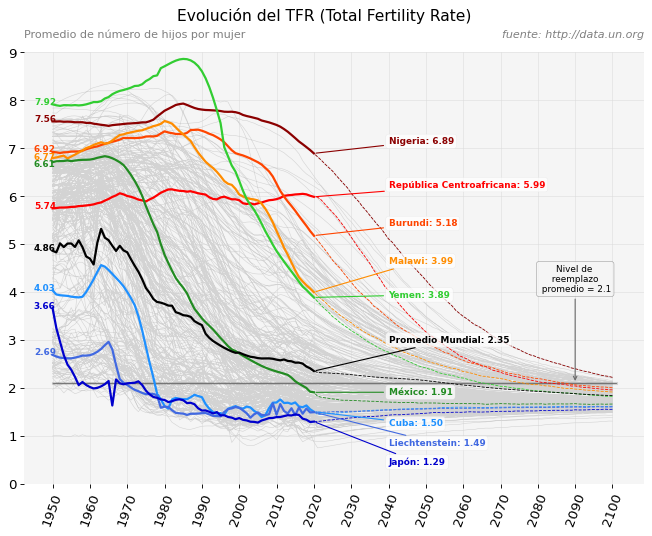
\includegraphics{04_Fertilidad_mundial_files/figure-pdf/cell-18-output-2.png}

\section{Exploración de los otros
datos.}\label{exploraciuxf3n-de-los-otros-datos.}

\begin{Shaded}
\begin{Highlighting}[]
\NormalTok{fig, ax }\OperatorTok{=}\NormalTok{ set\_canvas(LEB, }\StringTok{\textquotesingle{}Year(s)\textquotesingle{}}\NormalTok{, }\StringTok{\textquotesingle{}Value\textquotesingle{}}\NormalTok{, }\StringTok{\textquotesingle{}Country or Area\textquotesingle{}}\NormalTok{, (}\DecValTok{10}\NormalTok{,}\DecValTok{7}\NormalTok{), ystep}\OperatorTok{=}\DecValTok{10}\NormalTok{)}
\NormalTok{plot\_country(ax, LEB\_group.get\_group(}\StringTok{\textquotesingle{}Yemen\textquotesingle{}}\NormalTok{).dropna(), color}\OperatorTok{=}\StringTok{\textquotesingle{}C0\textquotesingle{}}\NormalTok{, label}\OperatorTok{=}\StringTok{\textquotesingle{}Yemen\textquotesingle{}}\NormalTok{, maxim}\OperatorTok{=}\DecValTok{2022}\NormalTok{)}
\NormalTok{plot\_country(ax, LEB\_group.get\_group(}\StringTok{\textquotesingle{}Mexico\textquotesingle{}}\NormalTok{).dropna(), color}\OperatorTok{=}\StringTok{\textquotesingle{}C1\textquotesingle{}}\NormalTok{, label}\OperatorTok{=}\StringTok{\textquotesingle{}México\textquotesingle{}}\NormalTok{, maxim}\OperatorTok{=}\DecValTok{2022}\NormalTok{)}
\NormalTok{plot\_country(ax, LEB\_group.get\_group(}\StringTok{\textquotesingle{}Germany\textquotesingle{}}\NormalTok{).dropna(), color}\OperatorTok{=}\StringTok{\textquotesingle{}C2\textquotesingle{}}\NormalTok{, label}\OperatorTok{=}\StringTok{\textquotesingle{}Alemania\textquotesingle{}}\NormalTok{)}
\NormalTok{plot\_country(ax, LEB\_group.get\_group(}\StringTok{\textquotesingle{}Holy See\textquotesingle{}}\NormalTok{).dropna(), color}\OperatorTok{=}\StringTok{\textquotesingle{}C3\textquotesingle{}}\NormalTok{, label}\OperatorTok{=}\StringTok{\textquotesingle{}El Baticano\textquotesingle{}}\NormalTok{)}
\NormalTok{plot\_country(ax, LEB\_group.get\_group(}\StringTok{\textquotesingle{}United States of America\textquotesingle{}}\NormalTok{).dropna(), color}\OperatorTok{=}\StringTok{\textquotesingle{}C4\textquotesingle{}}\NormalTok{, label}\OperatorTok{=}\StringTok{\textquotesingle{}USA\textquotesingle{}}\NormalTok{)}
\NormalTok{plot\_country(ax, LEB\_group.get\_group(}\StringTok{\textquotesingle{}Niger\textquotesingle{}}\NormalTok{).dropna(), color}\OperatorTok{=}\StringTok{\textquotesingle{}C5\textquotesingle{}}\NormalTok{, label}\OperatorTok{=}\StringTok{\textquotesingle{}Nigeria\textquotesingle{}}\NormalTok{)}
\NormalTok{plot\_country(ax, LEB\_group.get\_group(}\StringTok{\textquotesingle{}China, Hong Kong SAR\textquotesingle{}}\NormalTok{).dropna(), color}\OperatorTok{=}\StringTok{\textquotesingle{}C6\textquotesingle{}}\NormalTok{, label}\OperatorTok{=}\StringTok{\textquotesingle{}Hong Kong\textquotesingle{}}\NormalTok{)}
\NormalTok{plot\_country(ax, LEB\_group.get\_group(}\StringTok{\textquotesingle{}San Marino\textquotesingle{}}\NormalTok{).dropna(), color}\OperatorTok{=}\StringTok{\textquotesingle{}C8\textquotesingle{}}\NormalTok{, label}\OperatorTok{=}\StringTok{\textquotesingle{}San Marino\textquotesingle{}}\NormalTok{)}
\end{Highlighting}
\end{Shaded}

\begin{verbatim}
Máximo = 95.7552,    País : Monaco
Mínimo = 11.9951,    País : Cambodia
\end{verbatim}

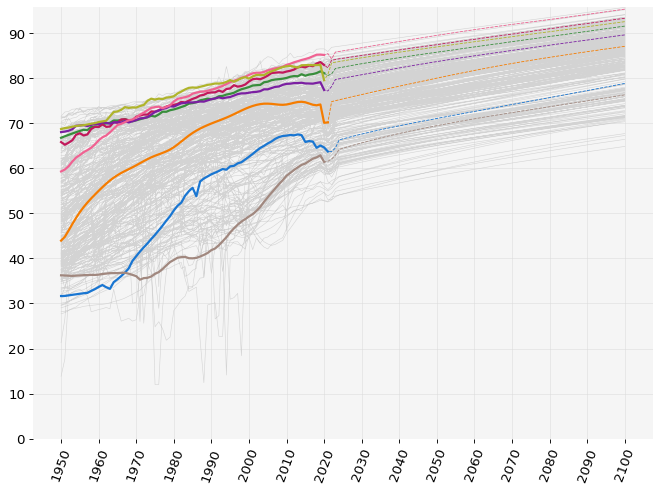
\includegraphics{04_Fertilidad_mundial_files/figure-pdf/cell-19-output-2.png}

\begin{Shaded}
\begin{Highlighting}[]
\NormalTok{maxmin(GDP, }\StringTok{\textquotesingle{}Year\textquotesingle{}}\NormalTok{, }\StringTok{\textquotesingle{}Value\textquotesingle{}}\NormalTok{, }\StringTok{\textquotesingle{}Country or Area\textquotesingle{}}\NormalTok{)}
\end{Highlighting}
\end{Shaded}

\begin{verbatim}
('Monaco', 234317.084818276, 'Viet Nam', 34.1125600868106, 1970, 2021)
\end{verbatim}

\begin{Shaded}
\begin{Highlighting}[]
\NormalTok{fig, ax }\OperatorTok{=}\NormalTok{ set\_canvas(GDP, }\StringTok{\textquotesingle{}Year\textquotesingle{}}\NormalTok{, }\StringTok{\textquotesingle{}Value\textquotesingle{}}\NormalTok{, }\StringTok{\textquotesingle{}Country or Area\textquotesingle{}}\NormalTok{, (}\DecValTok{10}\NormalTok{,}\DecValTok{7}\NormalTok{), xstep}\OperatorTok{=}\DecValTok{5}\NormalTok{, ystep}\OperatorTok{=}\DecValTok{10000}\NormalTok{)}
\NormalTok{plot\_country(ax, GDP\_group.get\_group(}\StringTok{\textquotesingle{}Yemen\textquotesingle{}}\NormalTok{).dropna(), time }\OperatorTok{=} \StringTok{\textquotesingle{}Year\textquotesingle{}}\NormalTok{, color}\OperatorTok{=}\StringTok{\textquotesingle{}C0\textquotesingle{}}\NormalTok{, label}\OperatorTok{=}\StringTok{\textquotesingle{}Yemen\textquotesingle{}}\NormalTok{, maxim}\OperatorTok{=}\DecValTok{2022}\NormalTok{)}
\NormalTok{plot\_country(ax, GDP\_group.get\_group(}\StringTok{\textquotesingle{}Mexico\textquotesingle{}}\NormalTok{).dropna(), time }\OperatorTok{=} \StringTok{\textquotesingle{}Year\textquotesingle{}}\NormalTok{, color}\OperatorTok{=}\StringTok{\textquotesingle{}C1\textquotesingle{}}\NormalTok{, label}\OperatorTok{=}\StringTok{\textquotesingle{}México\textquotesingle{}}\NormalTok{, maxim}\OperatorTok{=}\DecValTok{2022}\NormalTok{)}
\NormalTok{plot\_country(ax, GDP\_group.get\_group(}\StringTok{\textquotesingle{}Germany\textquotesingle{}}\NormalTok{).dropna(), time }\OperatorTok{=} \StringTok{\textquotesingle{}Year\textquotesingle{}}\NormalTok{, color}\OperatorTok{=}\StringTok{\textquotesingle{}C2\textquotesingle{}}\NormalTok{, label}\OperatorTok{=}\StringTok{\textquotesingle{}Alemania\textquotesingle{}}\NormalTok{)}
\CommentTok{\#plot\_country(ax, GDP\_group.get\_group(\textquotesingle{}Holy See\textquotesingle{}).dropna(), time = \textquotesingle{}Year\textquotesingle{}, color=\textquotesingle{}C3\textquotesingle{}, label=\textquotesingle{}El Baticano\textquotesingle{})}
\CommentTok{\#plot\_country(ax, GDP\_group.get\_group(\textquotesingle{}United States of America\textquotesingle{}).dropna(), time = \textquotesingle{}Year\textquotesingle{}, color=\textquotesingle{}C4\textquotesingle{}, label=\textquotesingle{}USA\textquotesingle{})}
\NormalTok{plot\_country(ax, GDP\_group.get\_group(}\StringTok{\textquotesingle{}Niger\textquotesingle{}}\NormalTok{).dropna(), time }\OperatorTok{=} \StringTok{\textquotesingle{}Year\textquotesingle{}}\NormalTok{, color}\OperatorTok{=}\StringTok{\textquotesingle{}C5\textquotesingle{}}\NormalTok{, label}\OperatorTok{=}\StringTok{\textquotesingle{}Nigeria\textquotesingle{}}\NormalTok{)}
\NormalTok{plot\_country(ax, GDP\_group.get\_group(}\StringTok{\textquotesingle{}China, Hong Kong SAR\textquotesingle{}}\NormalTok{).dropna(), time }\OperatorTok{=} \StringTok{\textquotesingle{}Year\textquotesingle{}}\NormalTok{, color}\OperatorTok{=}\StringTok{\textquotesingle{}C6\textquotesingle{}}\NormalTok{, label}\OperatorTok{=}\StringTok{\textquotesingle{}Hong Kong\textquotesingle{}}\NormalTok{)}
\NormalTok{plot\_country(ax, GDP\_group.get\_group(}\StringTok{\textquotesingle{}San Marino\textquotesingle{}}\NormalTok{).dropna(), time }\OperatorTok{=} \StringTok{\textquotesingle{}Year\textquotesingle{}}\NormalTok{, color}\OperatorTok{=}\StringTok{\textquotesingle{}C8\textquotesingle{}}\NormalTok{, label}\OperatorTok{=}\StringTok{\textquotesingle{}San Marino\textquotesingle{}}\NormalTok{)}
\end{Highlighting}
\end{Shaded}

\begin{verbatim}
Máximo = 234317.084818276,   País : Monaco
Mínimo = 34.1125600868106,   País : Viet Nam
\end{verbatim}

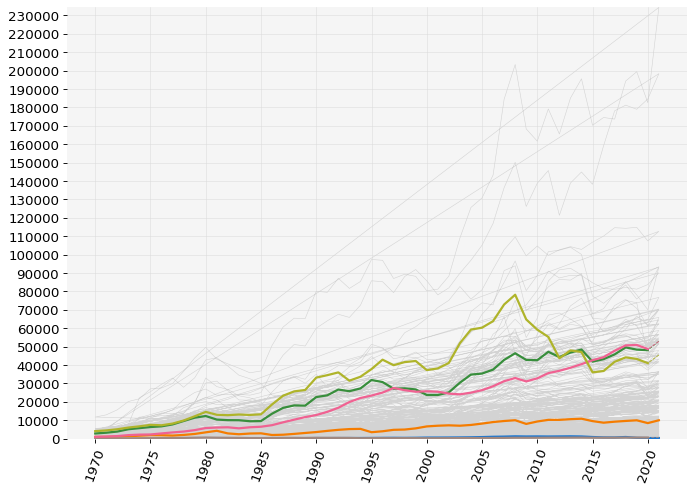
\includegraphics{04_Fertilidad_mundial_files/figure-pdf/cell-21-output-2.png}

\begin{Shaded}
\begin{Highlighting}[]
\NormalTok{maxmin(EDU, }\StringTok{\textquotesingle{}Time Period\textquotesingle{}}\NormalTok{, }\StringTok{\textquotesingle{}Observation Value\textquotesingle{}}\NormalTok{, }\StringTok{\textquotesingle{}Reference Area\textquotesingle{}}\NormalTok{)}
\end{Highlighting}
\end{Shaded}

\begin{verbatim}
('Cuba', 150.70758, 'Anguilla', 0.0, 1975, 2015)
\end{verbatim}

\begin{Shaded}
\begin{Highlighting}[]
\NormalTok{fig, ax }\OperatorTok{=}\NormalTok{ set\_canvas(EDU, }\StringTok{\textquotesingle{}Time Period\textquotesingle{}}\NormalTok{, }\StringTok{\textquotesingle{}Observation Value\textquotesingle{}}\NormalTok{, }\StringTok{\textquotesingle{}Reference Area\textquotesingle{}}\NormalTok{, (}\DecValTok{10}\NormalTok{,}\DecValTok{7}\NormalTok{), xstep}\OperatorTok{=}\DecValTok{5}\NormalTok{, ystep}\OperatorTok{=}\DecValTok{10}\NormalTok{)}
\NormalTok{plot\_country(ax, EDU\_group.get\_group(}\StringTok{\textquotesingle{}Yemen\textquotesingle{}}\NormalTok{).dropna(), time }\OperatorTok{=} \StringTok{\textquotesingle{}Time Period\textquotesingle{}}\NormalTok{, value }\OperatorTok{=} \StringTok{\textquotesingle{}Observation Value\textquotesingle{}}\NormalTok{, color}\OperatorTok{=}\StringTok{\textquotesingle{}C0\textquotesingle{}}\NormalTok{, label}\OperatorTok{=}\StringTok{\textquotesingle{}Yemen\textquotesingle{}}\NormalTok{, maxim}\OperatorTok{=}\DecValTok{2022}\NormalTok{)}
\NormalTok{plot\_country(ax, EDU\_group.get\_group(}\StringTok{\textquotesingle{}Mexico\textquotesingle{}}\NormalTok{).dropna(), time }\OperatorTok{=} \StringTok{\textquotesingle{}Time Period\textquotesingle{}}\NormalTok{, value }\OperatorTok{=} \StringTok{\textquotesingle{}Observation Value\textquotesingle{}}\NormalTok{, color}\OperatorTok{=}\StringTok{\textquotesingle{}C1\textquotesingle{}}\NormalTok{, label}\OperatorTok{=}\StringTok{\textquotesingle{}México\textquotesingle{}}\NormalTok{, maxim}\OperatorTok{=}\DecValTok{2022}\NormalTok{)}
\NormalTok{plot\_country(ax, EDU\_group.get\_group(}\StringTok{\textquotesingle{}Germany\textquotesingle{}}\NormalTok{).dropna(), time }\OperatorTok{=} \StringTok{\textquotesingle{}Time Period\textquotesingle{}}\NormalTok{, value }\OperatorTok{=} \StringTok{\textquotesingle{}Observation Value\textquotesingle{}}\NormalTok{, color}\OperatorTok{=}\StringTok{\textquotesingle{}C2\textquotesingle{}}\NormalTok{, label}\OperatorTok{=}\StringTok{\textquotesingle{}Alemania\textquotesingle{}}\NormalTok{)}
\CommentTok{\#plot\_country(ax, EDU\_group.get\_group(\textquotesingle{}Holy See\textquotesingle{}).dropna(), time = \textquotesingle{}Time Period\textquotesingle{}, value = \textquotesingle{}Observation Value\textquotesingle{}, color=\textquotesingle{}C3\textquotesingle{}, label=\textquotesingle{}El Baticano\textquotesingle{})}
\NormalTok{plot\_country(ax, EDU\_group.get\_group(}\StringTok{\textquotesingle{}United States of America\textquotesingle{}}\NormalTok{).dropna(), time }\OperatorTok{=} \StringTok{\textquotesingle{}Time Period\textquotesingle{}}\NormalTok{, value }\OperatorTok{=} \StringTok{\textquotesingle{}Observation Value\textquotesingle{}}\NormalTok{, color}\OperatorTok{=}\StringTok{\textquotesingle{}C4\textquotesingle{}}\NormalTok{, label}\OperatorTok{=}\StringTok{\textquotesingle{}USA\textquotesingle{}}\NormalTok{)}
\NormalTok{plot\_country(ax, EDU\_group.get\_group(}\StringTok{\textquotesingle{}Niger\textquotesingle{}}\NormalTok{).dropna(), time }\OperatorTok{=} \StringTok{\textquotesingle{}Time Period\textquotesingle{}}\NormalTok{, value }\OperatorTok{=} \StringTok{\textquotesingle{}Observation Value\textquotesingle{}}\NormalTok{, color}\OperatorTok{=}\StringTok{\textquotesingle{}C5\textquotesingle{}}\NormalTok{, label}\OperatorTok{=}\StringTok{\textquotesingle{}Nigeria\textquotesingle{}}\NormalTok{)}
\CommentTok{\#plot\_country(ax, EDU\_group.get\_group(\textquotesingle{}China, Hong Kong SAR\textquotesingle{}).dropna(), time = \textquotesingle{}Time Period\textquotesingle{}, value = \textquotesingle{}Observation Value\textquotesingle{}, color=\textquotesingle{}C6\textquotesingle{}, label=\textquotesingle{}Hong Kong\textquotesingle{})}
\NormalTok{plot\_country(ax, EDU\_group.get\_group(}\StringTok{\textquotesingle{}San Marino\textquotesingle{}}\NormalTok{).dropna(), time }\OperatorTok{=} \StringTok{\textquotesingle{}Time Period\textquotesingle{}}\NormalTok{, value }\OperatorTok{=} \StringTok{\textquotesingle{}Observation Value\textquotesingle{}}\NormalTok{, color}\OperatorTok{=}\StringTok{\textquotesingle{}C8\textquotesingle{}}\NormalTok{, label}\OperatorTok{=}\StringTok{\textquotesingle{}San Marino\textquotesingle{}}\NormalTok{)}
\end{Highlighting}
\end{Shaded}

\begin{verbatim}
Máximo = 150.70758,      País : Cuba
Mínimo = 0.0,    País : Anguilla
\end{verbatim}

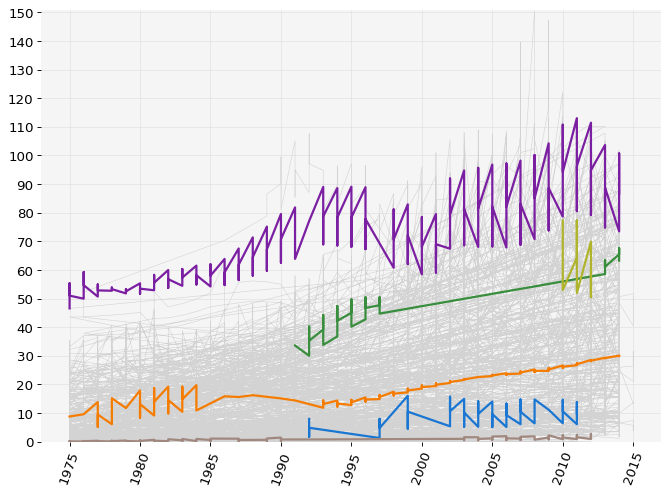
\includegraphics{04_Fertilidad_mundial_files/figure-pdf/cell-23-output-2.png}

\section{Construcción del HDI}\label{construcciuxf3n-del-hdi}

Se extrae información para el año 2010.

\begin{Shaded}
\begin{Highlighting}[]
\NormalTok{countries }\OperatorTok{=} \BuiltInTok{list}\NormalTok{(}\BuiltInTok{filter}\NormalTok{(filtra\_EDU, }\BuiltInTok{list}\NormalTok{(}\BuiltInTok{filter}\NormalTok{(filtra\_GDP, }\BuiltInTok{list}\NormalTok{(}\BuiltInTok{filter}\NormalTok{(filtra\_LEB, TFR\_countries))))))}
\NormalTok{tfr }\OperatorTok{=}\NormalTok{ pd.Series(dtype}\OperatorTok{=}\BuiltInTok{float}\NormalTok{)}
\NormalTok{gdp }\OperatorTok{=}\NormalTok{ pd.Series(dtype}\OperatorTok{=}\BuiltInTok{float}\NormalTok{)}
\NormalTok{edu }\OperatorTok{=}\NormalTok{ pd.Series(dtype}\OperatorTok{=}\BuiltInTok{float}\NormalTok{)}
\NormalTok{leb }\OperatorTok{=}\NormalTok{ pd.Series(dtype}\OperatorTok{=}\BuiltInTok{float}\NormalTok{)}
\NormalTok{final\_countries }\OperatorTok{=}\NormalTok{ []}
\NormalTok{año }\OperatorTok{=} \DecValTok{2010}

\NormalTok{paises\_to\_remove }\OperatorTok{=}\NormalTok{ [}\StringTok{\textquotesingle{}Malaysia\textquotesingle{}}\NormalTok{, }\StringTok{\textquotesingle{}British Virgin Islands\textquotesingle{}}\NormalTok{, }\StringTok{\textquotesingle{}Cook Islands\textquotesingle{}}\NormalTok{, }\StringTok{\textquotesingle{}Monaco\textquotesingle{}}\NormalTok{, }\StringTok{\textquotesingle{}Seychelles\textquotesingle{}}\NormalTok{]}
\ControlFlowTok{for}\NormalTok{ p }\KeywordTok{in}\NormalTok{ paises\_to\_remove:}
\NormalTok{    countries.remove(p)}

\ControlFlowTok{for}\NormalTok{ i, c }\KeywordTok{in} \BuiltInTok{enumerate}\NormalTok{(countries):}

\NormalTok{    c\_g }\OperatorTok{=}\NormalTok{ EDU\_group.get\_group(c).groupby(}\StringTok{\textquotesingle{}Sex\textquotesingle{}}\NormalTok{).get\_group(}\StringTok{\textquotesingle{}Female\textquotesingle{}}\NormalTok{)}
    \ControlFlowTok{if}\NormalTok{ año }\KeywordTok{in}\NormalTok{ c\_g[}\StringTok{\textquotesingle{}Time Period\textquotesingle{}}\NormalTok{].values:}
\NormalTok{        final\_countries.append(c)}
        
\NormalTok{        edu }\OperatorTok{=}\NormalTok{ pd.concat([edu, c\_g[c\_g[}\StringTok{\textquotesingle{}Time Period\textquotesingle{}}\NormalTok{] }\OperatorTok{==}\NormalTok{ año][}\StringTok{\textquotesingle{}Observation Value\textquotesingle{}}\NormalTok{]])}
    
\NormalTok{        c\_g }\OperatorTok{=}\NormalTok{ GDP\_group.get\_group(c)}
\NormalTok{        gdp }\OperatorTok{=}\NormalTok{ pd.concat([gdp, c\_g[c\_g[}\StringTok{\textquotesingle{}Year\textquotesingle{}}\NormalTok{] }\OperatorTok{==}\NormalTok{ año][}\StringTok{\textquotesingle{}Value\textquotesingle{}}\NormalTok{]])}
        
\NormalTok{        c\_g }\OperatorTok{=}\NormalTok{ TFR\_group.get\_group(c)}
\NormalTok{        tfr }\OperatorTok{=}\NormalTok{ pd.concat([tfr, c\_g[c\_g[}\StringTok{\textquotesingle{}Year(s)\textquotesingle{}}\NormalTok{] }\OperatorTok{==}\NormalTok{ año][}\StringTok{\textquotesingle{}Value\textquotesingle{}}\NormalTok{]])}
        
\NormalTok{        c\_g }\OperatorTok{=}\NormalTok{ LEB\_group.get\_group(c)}
\NormalTok{        leb }\OperatorTok{=}\NormalTok{ pd.concat([leb, c\_g[c\_g[}\StringTok{\textquotesingle{}Year(s)\textquotesingle{}}\NormalTok{] }\OperatorTok{==}\NormalTok{ año][}\StringTok{\textquotesingle{}Value\textquotesingle{}}\NormalTok{]])}
\end{Highlighting}
\end{Shaded}

\begin{Shaded}
\begin{Highlighting}[]
\BuiltInTok{print}\NormalTok{(}\BuiltInTok{len}\NormalTok{(tfr), }\BuiltInTok{len}\NormalTok{(gdp), }\BuiltInTok{len}\NormalTok{(edu), }\BuiltInTok{len}\NormalTok{(leb))}
\end{Highlighting}
\end{Shaded}

\begin{verbatim}
118 118 118 118
\end{verbatim}

Se construye el dataframe con todas las variables para los países donde
se tiene información.

\begin{Shaded}
\begin{Highlighting}[]
\NormalTok{hdi }\OperatorTok{=}\NormalTok{ pd.DataFrame()}
\NormalTok{hdi[}\StringTok{\textquotesingle{}País\textquotesingle{}}\NormalTok{] }\OperatorTok{=}\NormalTok{ final\_countries}
\NormalTok{hdi[}\StringTok{\textquotesingle{}TFR\textquotesingle{}}\NormalTok{] }\OperatorTok{=} \BuiltInTok{list}\NormalTok{(tfr)}
\NormalTok{hdi[}\StringTok{\textquotesingle{}GDP\textquotesingle{}}\NormalTok{] }\OperatorTok{=} \BuiltInTok{list}\NormalTok{(gdp)}
\NormalTok{hdi[}\StringTok{\textquotesingle{}EDU\textquotesingle{}}\NormalTok{] }\OperatorTok{=} \BuiltInTok{list}\NormalTok{(edu)}
\NormalTok{hdi[}\StringTok{\textquotesingle{}LEB\textquotesingle{}}\NormalTok{] }\OperatorTok{=} \BuiltInTok{list}\NormalTok{(leb)}
\NormalTok{hdi}
\end{Highlighting}
\end{Shaded}

\begin{longtable}[]{@{}llllll@{}}
\toprule\noalign{}
& País & TFR & GDP & EDU & LEB \\
\midrule\noalign{}
\endhead
\bottomrule\noalign{}
\endlastfoot
0 & Albania & 1.6564 & 4052.927488 & 52.38337 & 77.9359 \\
1 & Algeria & 2.8434 & 4493.635433 & 35.33614 & 73.8081 \\
2 & Antigua and Barbuda & 1.7854 & 13038.258604 & 22.67580 & 76.8195 \\
3 & Argentina & 2.3462 & 10023.206688 & 89.15845 & 75.7208 \\
4 & Armenia & 1.5010 & 3462.399904 & 63.13266 & 73.1597 \\
... & ... & ... & ... & ... & ... \\
113 & Uruguay & 2.0110 & 11567.565434 & 80.32340 & 76.8580 \\
114 & Uzbekistan & 2.4407 & 1789.707894 & 7.55595 & 69.2354 \\
115 & Viet Nam & 1.8949 & 1631.765100 & 22.71635 & 73.5126 \\
116 & Yemen & 4.8553 & 1179.830933 & 6.40428 & 67.2800 \\
117 & Zimbabwe & 4.0248 & 826.676632 & 5.23100 & 50.6523 \\
\end{longtable}

Se agrega una columna para el HDI.

\begin{Shaded}
\begin{Highlighting}[]
\NormalTok{hdi[}\StringTok{\textquotesingle{}HDI\textquotesingle{}}\NormalTok{] }\OperatorTok{=}\NormalTok{ np.cbrt(hdi.TFR }\OperatorTok{*}\NormalTok{ hdi.EDU }\OperatorTok{*}\NormalTok{ hdi.LEB)}
\end{Highlighting}
\end{Shaded}

\begin{Shaded}
\begin{Highlighting}[]
\NormalTok{hdi[}\StringTok{\textquotesingle{}HDI\textquotesingle{}}\NormalTok{] }\OperatorTok{=}\NormalTok{ hdi.HDI }\OperatorTok{/}\NormalTok{ hdi.HDI.}\BuiltInTok{max}\NormalTok{()}
\end{Highlighting}
\end{Shaded}

\begin{Shaded}
\begin{Highlighting}[]
\NormalTok{hdi}
\end{Highlighting}
\end{Shaded}

\begin{longtable}[]{@{}lllllll@{}}
\toprule\noalign{}
& País & TFR & GDP & EDU & LEB & HDI \\
\midrule\noalign{}
\endhead
\bottomrule\noalign{}
\endlastfoot
0 & Albania & 1.6564 & 4052.927488 & 52.38337 & 77.9359 & 0.719815 \\
1 & Algeria & 2.8434 & 4493.635433 & 35.33614 & 73.8081 & 0.742293 \\
2 & Antigua and Barbuda & 1.7854 & 13038.258604 & 22.67580 & 76.8195 &
0.555621 \\
3 & Argentina & 2.3462 & 10023.206688 & 89.15845 & 75.7208 & 0.955952 \\
4 & Armenia & 1.5010 & 3462.399904 & 63.13266 & 73.1597 & 0.725812 \\
... & ... & ... & ... & ... & ... & ... \\
113 & Uruguay & 2.0110 & 11567.565434 & 80.32340 & 76.8580 & 0.881393 \\
114 & Uzbekistan & 2.4407 & 1789.707894 & 7.55595 & 69.2354 &
0.412952 \\
115 & Viet Nam & 1.8949 & 1631.765100 & 22.71635 & 73.5126 & 0.558836 \\
116 & Yemen & 4.8553 & 1179.830933 & 6.40428 & 67.2800 & 0.486832 \\
117 & Zimbabwe & 4.0248 & 826.676632 & 5.23100 & 50.6523 & 0.388894 \\
\end{longtable}

Se realiza una regresión lineal del HDI vs TFR.

\begin{Shaded}
\begin{Highlighting}[]
\NormalTok{lres }\OperatorTok{=}\NormalTok{ scipy.stats.linregress(hdi.TFR, hdi.HDI)}
\BuiltInTok{print}\NormalTok{(lres.slope, lres.intercept, lres.rvalue}\OperatorTok{**}\DecValTok{2}\NormalTok{)}
\NormalTok{x }\OperatorTok{=}\NormalTok{ np.linspace(}\DecValTok{1}\NormalTok{,}\DecValTok{9}\NormalTok{,}\DecValTok{100}\NormalTok{)}
\NormalTok{y }\OperatorTok{=}\NormalTok{ lres.slope }\OperatorTok{*}\NormalTok{ x }\OperatorTok{+}\NormalTok{ lres.intercept}

\NormalTok{plt.plot(x, y, label}\OperatorTok{=}\StringTok{\textquotesingle{}Regresión lineal\textquotesingle{}}\NormalTok{)}
\NormalTok{plt.legend()}
\NormalTok{plt.show()}
\end{Highlighting}
\end{Shaded}

\begin{verbatim}
-0.08804520907984292 0.8975361617317406 0.5010566535168526
\end{verbatim}

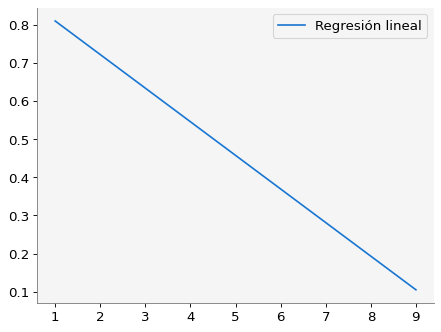
\includegraphics{04_Fertilidad_mundial_files/figure-pdf/cell-30-output-2.png}

Se grafica todo juntos

\begin{Shaded}
\begin{Highlighting}[]
\NormalTok{hdi.sort\_values(}\StringTok{\textquotesingle{}EDU\textquotesingle{}}\NormalTok{, inplace }\OperatorTok{=} \VariableTok{True}\NormalTok{)}

\NormalTok{lista\_paises }\OperatorTok{=}\NormalTok{ [(}\StringTok{\textquotesingle{}Niger\textquotesingle{}}\NormalTok{, }\StringTok{\textquotesingle{}Nigeria\textquotesingle{}}\NormalTok{, }\StringTok{\textquotesingle{}darkred\textquotesingle{}}\NormalTok{), }
\NormalTok{             (}\StringTok{\textquotesingle{}Central African Republic\textquotesingle{}}\NormalTok{, }\StringTok{\textquotesingle{}República Centroafricana\textquotesingle{}}\NormalTok{, }\StringTok{\textquotesingle{}red\textquotesingle{}}\NormalTok{),}
\NormalTok{             (}\StringTok{\textquotesingle{}Burundi\textquotesingle{}}\NormalTok{, }\StringTok{\textquotesingle{}Burundi\textquotesingle{}}\NormalTok{, }\StringTok{\textquotesingle{}orangered\textquotesingle{}}\NormalTok{),}
\NormalTok{             (}\StringTok{\textquotesingle{}Malawi\textquotesingle{}}\NormalTok{, }\StringTok{\textquotesingle{}Malawi\textquotesingle{}}\NormalTok{, }\StringTok{\textquotesingle{}darkorange\textquotesingle{}}\NormalTok{),}
\NormalTok{             (}\StringTok{\textquotesingle{}Yemen\textquotesingle{}}\NormalTok{, }\StringTok{\textquotesingle{}Yemen\textquotesingle{}}\NormalTok{, }\StringTok{\textquotesingle{}limegreen\textquotesingle{}}\NormalTok{), }
\NormalTok{             (}\StringTok{\textquotesingle{}Mexico\textquotesingle{}}\NormalTok{, }\StringTok{\textquotesingle{}México\textquotesingle{}}\NormalTok{, }\StringTok{\textquotesingle{}forestgreen\textquotesingle{}}\NormalTok{),}
\NormalTok{             (}\StringTok{\textquotesingle{}Cuba\textquotesingle{}}\NormalTok{, }\StringTok{\textquotesingle{}Cuba\textquotesingle{}}\NormalTok{, }\StringTok{\textquotesingle{}dodgerblue\textquotesingle{}}\NormalTok{),}
\NormalTok{             (}\StringTok{\textquotesingle{}Liechtenstein\textquotesingle{}}\NormalTok{, }\StringTok{\textquotesingle{}Liechtenstein\textquotesingle{}}\NormalTok{, }\StringTok{\textquotesingle{}royalblue\textquotesingle{}}\NormalTok{),}
\NormalTok{             (}\StringTok{\textquotesingle{}Japan\textquotesingle{}}\NormalTok{, }\StringTok{\textquotesingle{}Japón\textquotesingle{}}\NormalTok{, }\StringTok{\textquotesingle{}mediumblue\textquotesingle{}}\NormalTok{)}
\NormalTok{               ]}

\NormalTok{paises\_to\_plot }\OperatorTok{=}\NormalTok{ [hdi[hdi[}\StringTok{\textquotesingle{}País\textquotesingle{}}\NormalTok{] }\OperatorTok{==}\NormalTok{ p[}\DecValTok{0}\NormalTok{]] }\ControlFlowTok{for}\NormalTok{ p }\KeywordTok{in}\NormalTok{ lista\_paises]}

\NormalTok{plt.figure(figsize}\OperatorTok{=}\NormalTok{(}\DecValTok{12}\NormalTok{,}\DecValTok{8}\NormalTok{))}

\NormalTok{ax }\OperatorTok{=}\NormalTok{ plt.subplot(}\DecValTok{111}\NormalTok{)}
\NormalTok{niv\_edu }\OperatorTok{=}\NormalTok{ np.array(hdi[}\StringTok{\textquotesingle{}EDU\textquotesingle{}}\NormalTok{]}\OperatorTok{*}\FloatTok{10.0}\NormalTok{)}
\CommentTok{\#gdp\_val = np.array(np.log(hdi[\textquotesingle{}GDP\textquotesingle{}]))}
\NormalTok{gdp\_val }\OperatorTok{=}\NormalTok{ np.array(hdi[}\StringTok{\textquotesingle{}GDP\textquotesingle{}}\NormalTok{])}

\NormalTok{scatter }\OperatorTok{=}\NormalTok{ ax.scatter(hdi[}\StringTok{\textquotesingle{}TFR\textquotesingle{}}\NormalTok{], hdi[}\StringTok{\textquotesingle{}HDI\textquotesingle{}}\NormalTok{], marker}\OperatorTok{=}\StringTok{\textquotesingle{}o\textquotesingle{}}\NormalTok{, s}\OperatorTok{=}\NormalTok{niv\_edu, c}\OperatorTok{=}\NormalTok{gdp\_val, ec}\OperatorTok{=}\StringTok{\textquotesingle{}silver\textquotesingle{}}\NormalTok{, cmap}\OperatorTok{=}\StringTok{\textquotesingle{}YlGnBu\textquotesingle{}}\NormalTok{, alpha}\OperatorTok{=}\FloatTok{0.75}\NormalTok{)}

\NormalTok{ha }\OperatorTok{=} \StringTok{\textquotesingle{}right\textquotesingle{}}
\ControlFlowTok{for}\NormalTok{ pa, cl }\KeywordTok{in} \BuiltInTok{zip}\NormalTok{(paises\_to\_plot, lista\_paises):}
    \ControlFlowTok{if}\NormalTok{ cl[}\DecValTok{0}\NormalTok{] }\OperatorTok{==} \StringTok{\textquotesingle{}Yemen\textquotesingle{}}\NormalTok{:}
\NormalTok{        xt, yt }\OperatorTok{=} \FloatTok{6.}\NormalTok{, }\FloatTok{0.55}
    \ControlFlowTok{elif}\NormalTok{ cl[}\DecValTok{0}\NormalTok{] }\OperatorTok{==} \StringTok{\textquotesingle{}Niger\textquotesingle{}}\NormalTok{:}
\NormalTok{        xt, yt }\OperatorTok{=} \DecValTok{8}\NormalTok{, }\FloatTok{0.4}
    \ControlFlowTok{elif}\NormalTok{ cl[}\DecValTok{0}\NormalTok{] }\OperatorTok{==} \StringTok{\textquotesingle{}India\textquotesingle{}}\NormalTok{:}
\NormalTok{        xt, yt }\OperatorTok{=} \FloatTok{3.0}\NormalTok{, }\FloatTok{0.2}
    \ControlFlowTok{elif}\NormalTok{ cl[}\DecValTok{0}\NormalTok{] }\OperatorTok{==} \StringTok{\textquotesingle{}Yemen\textquotesingle{}}\NormalTok{:}
\NormalTok{        xt, yt }\OperatorTok{=} \FloatTok{4.5}\NormalTok{, }\FloatTok{1.0}
    \ControlFlowTok{elif}\NormalTok{ cl[}\DecValTok{0}\NormalTok{] }\OperatorTok{==} \StringTok{\textquotesingle{}Mexico\textquotesingle{}}\NormalTok{:}
\NormalTok{        xt, yt }\OperatorTok{=} \FloatTok{2.25}\NormalTok{, }\FloatTok{.25}
    \ControlFlowTok{elif}\NormalTok{ cl[}\DecValTok{0}\NormalTok{] }\OperatorTok{==} \StringTok{\textquotesingle{}Liechtenstein\textquotesingle{}}\NormalTok{:}
\NormalTok{        xt, yt }\OperatorTok{=} \FloatTok{0.75}\NormalTok{, }\FloatTok{0.35}
\NormalTok{        ha }\OperatorTok{=} \StringTok{\textquotesingle{}left\textquotesingle{}}
    \ControlFlowTok{elif}\NormalTok{ cl[}\DecValTok{0}\NormalTok{] }\OperatorTok{==} \StringTok{\textquotesingle{}Burundi\textquotesingle{}}\NormalTok{:}
\NormalTok{        xt, yt }\OperatorTok{=} \FloatTok{6.75}\NormalTok{, }\FloatTok{0.45}
    \ControlFlowTok{elif}\NormalTok{ cl[}\DecValTok{0}\NormalTok{] }\OperatorTok{==} \StringTok{\textquotesingle{}Central African Republic\textquotesingle{}}\NormalTok{:}
\NormalTok{        xt, yt }\OperatorTok{=} \DecValTok{7}\NormalTok{, }\FloatTok{0.1}
    \ControlFlowTok{elif}\NormalTok{ cl[}\DecValTok{0}\NormalTok{] }\OperatorTok{==} \StringTok{\textquotesingle{}Malawi\textquotesingle{}}\NormalTok{:}
\NormalTok{        xt, yt }\OperatorTok{=} \DecValTok{4}\NormalTok{, }\FloatTok{0.1}
    \ControlFlowTok{elif}\NormalTok{ cl[}\DecValTok{0}\NormalTok{] }\OperatorTok{==} \StringTok{\textquotesingle{}Republic of Korea\textquotesingle{}}\NormalTok{:}
\NormalTok{        xt, yt }\OperatorTok{=} \FloatTok{0.65}\NormalTok{, }\FloatTok{1.05}
    \ControlFlowTok{elif}\NormalTok{ cl[}\DecValTok{0}\NormalTok{] }\OperatorTok{==} \StringTok{\textquotesingle{}Cuba\textquotesingle{}}\NormalTok{:}
\NormalTok{        xt, yt }\OperatorTok{=} \DecValTok{3}\NormalTok{, }\FloatTok{1.05}
    \ControlFlowTok{else}\NormalTok{:}
\NormalTok{        xt, yt }\OperatorTok{=} \FloatTok{0.75}\NormalTok{, }\FloatTok{1.0}

\NormalTok{    niv\_edu }\OperatorTok{=}\NormalTok{ np.array(pa[}\StringTok{\textquotesingle{}EDU\textquotesingle{}}\NormalTok{]}\OperatorTok{*}\FloatTok{10.0}\NormalTok{)}
\NormalTok{    gdp\_val }\OperatorTok{=}\NormalTok{ np.array(np.log(pa[}\StringTok{\textquotesingle{}GDP\textquotesingle{}}\NormalTok{]))}
\NormalTok{    ax.scatter(pa[}\StringTok{\textquotesingle{}TFR\textquotesingle{}}\NormalTok{], pa[}\StringTok{\textquotesingle{}HDI\textquotesingle{}}\NormalTok{], marker}\OperatorTok{=}\StringTok{\textquotesingle{}o\textquotesingle{}}\NormalTok{, s }\OperatorTok{=}\NormalTok{ niv\_edu, ec}\OperatorTok{=}\NormalTok{cl[}\DecValTok{2}\NormalTok{], facecolor}\OperatorTok{=}\StringTok{"None"}\NormalTok{, alpha}\OperatorTok{=}\FloatTok{0.1}\NormalTok{, zorder}\OperatorTok{=}\DecValTok{15}\NormalTok{)}

\NormalTok{    plt.annotate(cl[}\DecValTok{1}\NormalTok{], xy }\OperatorTok{=}\NormalTok{ (pa[}\StringTok{\textquotesingle{}TFR\textquotesingle{}}\NormalTok{], pa[}\StringTok{\textquotesingle{}HDI\textquotesingle{}}\NormalTok{]), xytext }\OperatorTok{=}\NormalTok{ (xt, yt), zorder}\OperatorTok{=}\DecValTok{20}\NormalTok{,}
\NormalTok{                     color }\OperatorTok{=}\NormalTok{ cl[}\DecValTok{2}\NormalTok{], fontsize}\OperatorTok{=}\DecValTok{10}\NormalTok{, fontweight}\OperatorTok{=}\StringTok{\textquotesingle{}normal\textquotesingle{}}\NormalTok{, ha}\OperatorTok{=}\NormalTok{ha,}
\NormalTok{                     bbox}\OperatorTok{=}\BuiltInTok{dict}\NormalTok{(boxstyle}\OperatorTok{=}\StringTok{\textquotesingle{}round\textquotesingle{}}\NormalTok{, fc}\OperatorTok{=}\StringTok{\textquotesingle{}white\textquotesingle{}}\NormalTok{, ec}\OperatorTok{=}\StringTok{\textquotesingle{}gainsboro\textquotesingle{}}\NormalTok{, alpha}\OperatorTok{=}\FloatTok{0.75}\NormalTok{, linewidth}\OperatorTok{=}\FloatTok{0.25}\NormalTok{),}
\NormalTok{                     arrowprops}\OperatorTok{=}\BuiltInTok{dict}\NormalTok{(arrowstyle}\OperatorTok{=}\StringTok{\textquotesingle{}{-}\textgreater{}\textquotesingle{}}\NormalTok{, color}\OperatorTok{=}\NormalTok{cl[}\DecValTok{2}\NormalTok{]))}
    
\NormalTok{ax.plot(x,y,}\StringTok{\textquotesingle{}k{-}{-}\textquotesingle{}}\NormalTok{, alpha}\OperatorTok{=}\FloatTok{0.5}\NormalTok{, lw}\OperatorTok{=}\DecValTok{3}\NormalTok{, label}\OperatorTok{=}\StringTok{\textquotesingle{}Ajuste: slope = }\SpecialCharTok{\{:0.3f\}}\StringTok{, intercept = }\SpecialCharTok{\{:0.3f\}}\StringTok{, PCC = }\SpecialCharTok{\{:0.3f\}}\StringTok{\textquotesingle{}}\NormalTok{.}\BuiltInTok{format}\NormalTok{(lres.slope, lres.intercept, lres.rvalue))}
\NormalTok{ax.set\_xlabel(}\StringTok{\textquotesingle{}TFR\textquotesingle{}}\NormalTok{)}
\NormalTok{ax.set\_ylabel(}\StringTok{\textquotesingle{}HDI\textquotesingle{}}\NormalTok{)}
\NormalTok{ax.set\_xticks([i }\ControlFlowTok{for}\NormalTok{ i }\KeywordTok{in} \BuiltInTok{range}\NormalTok{(}\DecValTok{1}\NormalTok{,}\DecValTok{10}\NormalTok{)], labels}\OperatorTok{=}\NormalTok{[i }\ControlFlowTok{for}\NormalTok{ i }\KeywordTok{in} \BuiltInTok{range}\NormalTok{(}\DecValTok{1}\NormalTok{,}\DecValTok{10}\NormalTok{)], fontsize}\OperatorTok{=}\DecValTok{14}\NormalTok{ )}
\NormalTok{ax.set\_yticks([}\DecValTok{0}\NormalTok{,}\FloatTok{0.2}\NormalTok{,}\FloatTok{0.4}\NormalTok{,}\FloatTok{0.6}\NormalTok{,}\FloatTok{0.8}\NormalTok{,}\FloatTok{1.0}\NormalTok{], labels}\OperatorTok{=}\NormalTok{[}\DecValTok{0}\NormalTok{,}\FloatTok{0.2}\NormalTok{,}\FloatTok{0.4}\NormalTok{,}\FloatTok{0.6}\NormalTok{,}\FloatTok{0.8}\NormalTok{,}\FloatTok{1.0}\NormalTok{], fontsize}\OperatorTok{=}\DecValTok{14}\NormalTok{)}
\NormalTok{ax.set\_ylim(}\OperatorTok{{-}}\FloatTok{0.1}\NormalTok{, }\FloatTok{1.1}\NormalTok{)}
\NormalTok{ax.spines[}\StringTok{\textquotesingle{}bottom\textquotesingle{}}\NormalTok{].set\_visible(}\VariableTok{False}\NormalTok{)}
\NormalTok{ax.grid(lw}\OperatorTok{=}\FloatTok{0.5}\NormalTok{)}
\NormalTok{ax.set\_title(}\StringTok{\textquotesingle{}Efecto del TFR, GDP y EDU en el HDI\textquotesingle{}}\NormalTok{, loc}\OperatorTok{=}\StringTok{\textquotesingle{}left\textquotesingle{}}\NormalTok{, color}\OperatorTok{=}\StringTok{\textquotesingle{}gray\textquotesingle{}}\NormalTok{, fontsize}\OperatorTok{=}\DecValTok{10}\NormalTok{)}
\NormalTok{ax.set\_title(}\StringTok{\textquotesingle{}fuente: http://data.un.org\textquotesingle{}}\NormalTok{, loc}\OperatorTok{=}\StringTok{\textquotesingle{}right\textquotesingle{}}\NormalTok{, color}\OperatorTok{=}\StringTok{\textquotesingle{}gray\textquotesingle{}}\NormalTok{, fontstyle}\OperatorTok{=}\StringTok{\textquotesingle{}italic\textquotesingle{}}\NormalTok{, fontsize}\OperatorTok{=}\DecValTok{10}\NormalTok{)}
\NormalTok{plt.suptitle(}\StringTok{\textquotesingle{}Índice de desarrollo humano (HDI) en 2010\textquotesingle{}}\NormalTok{, y }\OperatorTok{=} \FloatTok{0.96}\NormalTok{, color}\OperatorTok{=}\StringTok{\textquotesingle{}black\textquotesingle{}}\NormalTok{, fontsize}\OperatorTok{=}\DecValTok{14}\NormalTok{)}
\NormalTok{texto }\OperatorTok{=} \StringTok{""" }
\StringTok{Cada círculo representa a un país. El nivel de}
\StringTok{educación (EDU) en las mujeres se representa }
\StringTok{como el tamaño de cada círculo.}
\StringTok{"""}
\NormalTok{plt.text(}\FloatTok{5.5}\NormalTok{,}\FloatTok{0.9}\NormalTok{,texto, fontsize}\OperatorTok{=}\DecValTok{10}\NormalTok{,bbox}\OperatorTok{=}\BuiltInTok{dict}\NormalTok{(boxstyle}\OperatorTok{=}\StringTok{\textquotesingle{}round\textquotesingle{}}\NormalTok{, fc}\OperatorTok{=}\StringTok{\textquotesingle{}white\textquotesingle{}}\NormalTok{, ec}\OperatorTok{=}\StringTok{\textquotesingle{}silver\textquotesingle{}}\NormalTok{, alpha}\OperatorTok{=}\FloatTok{0.5}\NormalTok{, linewidth}\OperatorTok{=}\FloatTok{0.75}\NormalTok{))}
\NormalTok{plt.colorbar(mappable}\OperatorTok{=}\NormalTok{scatter, label}\OperatorTok{=}\StringTok{\textquotesingle{}GDP [USD $]\textquotesingle{}}\NormalTok{, ticks}\OperatorTok{=}\NormalTok{[}\DecValTok{1000}\NormalTok{, }\DecValTok{20000}\NormalTok{, }\DecValTok{40000}\NormalTok{, }\DecValTok{60000}\NormalTok{, }\DecValTok{80000}\NormalTok{, }\DecValTok{100000}\NormalTok{, }\DecValTok{120000}\NormalTok{, }\DecValTok{135000}\NormalTok{])}
\NormalTok{plt.legend(loc}\OperatorTok{=}\StringTok{\textquotesingle{}lower left\textquotesingle{}}\NormalTok{, frameon}\OperatorTok{=}\VariableTok{True}\NormalTok{)}

\NormalTok{plt.savefig(}\StringTok{\textquotesingle{}HDI.pdf\textquotesingle{}}\NormalTok{, dpi }\OperatorTok{=} \DecValTok{300}\NormalTok{)}
\end{Highlighting}
\end{Shaded}

\begin{verbatim}
/opt/conda/lib/python3.11/site-packages/matplotlib/text.py:1461: FutureWarning: Calling float on a single element Series is deprecated and will raise a TypeError in the future. Use float(ser.iloc[0]) instead
  x = float(self.convert_xunits(x))
/opt/conda/lib/python3.11/site-packages/matplotlib/text.py:1463: FutureWarning: Calling float on a single element Series is deprecated and will raise a TypeError in the future. Use float(ser.iloc[0]) instead
  y = float(self.convert_yunits(y))
/opt/conda/lib/python3.11/site-packages/matplotlib/text.py:1461: FutureWarning: Calling float on a single element Series is deprecated and will raise a TypeError in the future. Use float(ser.iloc[0]) instead
  x = float(self.convert_xunits(x))
/opt/conda/lib/python3.11/site-packages/matplotlib/text.py:1463: FutureWarning: Calling float on a single element Series is deprecated and will raise a TypeError in the future. Use float(ser.iloc[0]) instead
  y = float(self.convert_yunits(y))
\end{verbatim}

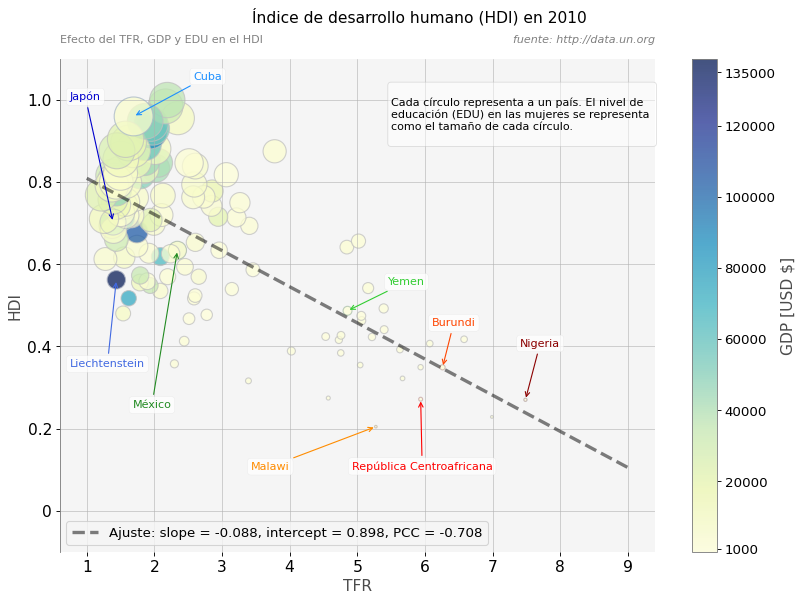
\includegraphics{04_Fertilidad_mundial_files/figure-pdf/cell-31-output-2.png}

\bookmarksetup{startatroot}

\chapter{Quizz 2. Mínimos
Cuadrados}\label{quizz-2.-muxednimos-cuadrados}

\textbf{Objetivo}.

\begin{itemize}
\tightlist
\item
  Entender en qué consiste el ajuste de rectas por el método de mínimos
  cuadrados.
\item
  Realizar una implementación de las matemáticas requeridas en este
  método.
\item
  Probar la implementación con datos generados de manera sintética.
\end{itemize}

Mínimos cuadrados by Luis M. de la Cruz is licensed under
Attribution-ShareAlike 4.0 International

\textbf{Trabajo realizado con el apoyo del Programa UNAM-DGAPA-PAPIME
PE101922}

\bookmarksetup{startatroot}

\chapter{Introducción.}\label{introducciuxf3n.}

El \textbf{método de mínimos cuadrados} se utiliza para ajustar rectas a
series de datos presentados en la forma \((x, y)\) como en la siguiente
tabla:

\begin{longtable}[]{@{}lllll@{}}
\toprule\noalign{}
\(x_0\) & \(x_1\) & \(x_2\) & \(\dots\) & \(x_N\) \\
\midrule\noalign{}
\endhead
\bottomrule\noalign{}
\endlastfoot
\(y_0\) & \(y_1\) & \(y_2\) & \(\dots\) & \(y_N\) \\
\end{longtable}

Este tipo de datos pueden provenir de diferentes fuentes como estudios
geofísicos en campo, estudios experimentales en laboratorio, obtención
de datos mediante encuestas, observación de fenómenos naturales, etc. La
idea es estudiar como una variable depende de la otra.

Una posibilidad es que la variación sea lineal es decir:
\(y = m x + b\).

Sin embargo, en la mayoría de los casos no es posible obtener una recta
exacta que pase por todos los puntos.

Para ello, el método de mínimos cuadrados nos proporciona con una
metodología para obtener la mejor recta que represente a todos los
puntos del conjunto de datos.

\bookmarksetup{startatroot}

\chapter{Conjuntos de datos.}\label{conjuntos-de-datos.-1}

Para esta actividad vamos a generar de manera sintética 4 conjuntos de
datos. Usaremos la función \texttt{np.random.rand()} de numpy.

\begin{Shaded}
\begin{Highlighting}[]
\ImportTok{import}\NormalTok{ numpy }\ImportTok{as}\NormalTok{ np}
\ImportTok{import}\NormalTok{ matplotlib.pyplot }\ImportTok{as}\NormalTok{ plt}
\ImportTok{from}\NormalTok{ macti.evaluation }\ImportTok{import} \OperatorTok{*}
\end{Highlighting}
\end{Shaded}

\begin{Shaded}
\begin{Highlighting}[]
\NormalTok{quizz }\OperatorTok{=}\NormalTok{ Quizz(}\StringTok{\textquotesingle{}q2\textquotesingle{}}\NormalTok{, }\StringTok{\textquotesingle{}HeCompA\textquotesingle{}}\NormalTok{, }\StringTok{\textquotesingle{}local\textquotesingle{}}\NormalTok{)}
\end{Highlighting}
\end{Shaded}

\begin{Shaded}
\begin{Highlighting}[]
\CommentTok{\# Total de datos de cada conjunto}
\NormalTok{N }\OperatorTok{=} \DecValTok{20}

\CommentTok{\# Fijamos la semilla para obtener los mismos valores siempre}
\NormalTok{np.random.seed(}\DecValTok{0}\NormalTok{)}

\CommentTok{\# Conjunto 0}
\NormalTok{x0 }\OperatorTok{=}\NormalTok{ np.linspace(}\DecValTok{0}\NormalTok{,}\DecValTok{10}\NormalTok{,N) }
\NormalTok{y0 }\OperatorTok{=}\NormalTok{ x0 }\OperatorTok{+}\NormalTok{ np.random.randn(N)}\OperatorTok{*}\DecValTok{2}

\CommentTok{\# Conjunto 1}
\NormalTok{x1 }\OperatorTok{=}\NormalTok{ np.random.randn(}\BuiltInTok{len}\NormalTok{(x0))}\OperatorTok{*}\DecValTok{10}
\NormalTok{y1 }\OperatorTok{=}\NormalTok{ np.random.randn(}\BuiltInTok{len}\NormalTok{(x0))}\OperatorTok{*}\DecValTok{10}

\CommentTok{\# Conjunto 2}
\NormalTok{x2 }\OperatorTok{=}\NormalTok{ np.arange(}\DecValTok{0}\NormalTok{,N)}\OperatorTok{*}\DecValTok{100}
\NormalTok{y2 }\OperatorTok{=} \OperatorTok{{-}}\NormalTok{x2 }\OperatorTok{+}\NormalTok{ np.random.randn(N)}\OperatorTok{*}\DecValTok{500}

\CommentTok{\# Conjunto 3}
\NormalTok{x3 }\OperatorTok{=}\NormalTok{ np.array([i }\ControlFlowTok{for}\NormalTok{ i }\KeywordTok{in} \BuiltInTok{range}\NormalTok{(N)])}
\NormalTok{y3 }\OperatorTok{=}\NormalTok{ np.random.rand(N)}\OperatorTok{*}\FloatTok{0.5}\OperatorTok{{-}}\FloatTok{0.5}
\end{Highlighting}
\end{Shaded}

\begin{Shaded}
\begin{Highlighting}[]
\BuiltInTok{print}\NormalTok{(}\StringTok{\textquotesingle{}}\CharTok{\textbackslash{}n}\StringTok{Arreglo x0 :}\CharTok{\textbackslash{}n}\SpecialCharTok{\{\}}\StringTok{\textquotesingle{}}\NormalTok{.}\BuiltInTok{format}\NormalTok{(x0))}
\BuiltInTok{print}\NormalTok{(}\StringTok{\textquotesingle{}Arreglo y0 :}\CharTok{\textbackslash{}n}\SpecialCharTok{\{\}}\StringTok{\textquotesingle{}}\NormalTok{.}\BuiltInTok{format}\NormalTok{(y0))}

\BuiltInTok{print}\NormalTok{(}\StringTok{\textquotesingle{}}\CharTok{\textbackslash{}n}\StringTok{Arreglo x1 :}\CharTok{\textbackslash{}n}\SpecialCharTok{\{\}}\StringTok{\textquotesingle{}}\NormalTok{.}\BuiltInTok{format}\NormalTok{(x1))}
\BuiltInTok{print}\NormalTok{(}\StringTok{\textquotesingle{}Arreglo y1 :}\CharTok{\textbackslash{}n}\SpecialCharTok{\{\}}\StringTok{\textquotesingle{}}\NormalTok{.}\BuiltInTok{format}\NormalTok{(y1))}

\BuiltInTok{print}\NormalTok{(}\StringTok{\textquotesingle{}}\CharTok{\textbackslash{}n}\StringTok{Arreglo x2 :}\CharTok{\textbackslash{}n}\SpecialCharTok{\{\}}\StringTok{\textquotesingle{}}\NormalTok{.}\BuiltInTok{format}\NormalTok{(x2))}
\BuiltInTok{print}\NormalTok{(}\StringTok{\textquotesingle{}Arreglo y2 :}\CharTok{\textbackslash{}n}\SpecialCharTok{\{\}}\StringTok{\textquotesingle{}}\NormalTok{.}\BuiltInTok{format}\NormalTok{(y2))}

\BuiltInTok{print}\NormalTok{(}\StringTok{\textquotesingle{}}\CharTok{\textbackslash{}n}\StringTok{Arreglo x3 :}\CharTok{\textbackslash{}n}\SpecialCharTok{\{\}}\StringTok{\textquotesingle{}}\NormalTok{.}\BuiltInTok{format}\NormalTok{(x3))}
\BuiltInTok{print}\NormalTok{(}\StringTok{\textquotesingle{}Arreglo y3 :}\CharTok{\textbackslash{}n}\SpecialCharTok{\{\}}\StringTok{\textquotesingle{}}\NormalTok{.}\BuiltInTok{format}\NormalTok{(y3))}
\end{Highlighting}
\end{Shaded}

\begin{verbatim}

Arreglo x0 :
[ 0.          0.52631579  1.05263158  1.57894737  2.10526316  2.63157895
  3.15789474  3.68421053  4.21052632  4.73684211  5.26315789  5.78947368
  6.31578947  6.84210526  7.36842105  7.89473684  8.42105263  8.94736842
  9.47368421 10.        ]
Arreglo y0 :
[ 3.52810469  1.32663021  3.01010755  6.06073377  5.84037914  0.67702319
  5.05807157  3.38149611  4.00408861  5.55803911  5.55124504  8.6980207
  7.83786492  7.0854553   8.25614752  8.5620855  11.40921078  8.53705189
 10.09981961  8.29180852]

Arreglo x1 :
[-25.52989816   6.53618595   8.64436199  -7.4216502   22.69754624
 -14.54365675   0.45758517  -1.8718385   15.32779214  14.6935877
   1.54947426   3.7816252   -8.87785748 -19.80796468  -3.47912149
   1.56348969  12.30290681  12.02379849  -3.87326817  -3.02302751]
Arreglo y1 :
[-10.48552965 -14.20017937 -17.06270191  19.50775395  -5.09652182
  -4.38074302 -12.5279536    7.77490356 -16.13897848  -2.1274028
  -8.95466561   3.86902498  -5.10805138 -11.80632184  -0.28182228
   4.28331871   0.66517222   3.02471898  -6.34322094  -3.62741166]

Arreglo x2 :
[   0  100  200  300  400  500  600  700  800  900 1000 1100 1200 1300
 1400 1500 1600 1700 1800 1900]
Arreglo y2 :
[ -336.23022389  -279.77658077  -606.57314102 -1163.14130117
  -311.28692887  -700.8904681  -1415.09917348  -468.60887224
 -1253.64918219  -874.0273021   -635.45471891 -1035.50854462
  -630.29965773 -1917.41291018 -1198.82917941 -1842.40504547
 -2035.39857459 -1989.42483238 -1955.77626606 -1871.91732889]

Arreglo x3 :
[ 0  1  2  3  4  5  6  7  8  9 10 11 12 13 14 15 16 17 18 19]
Arreglo y3 :
[-0.08552999 -0.49765226 -0.16109173 -0.36499601 -0.13240299 -0.01890573
 -0.37562343 -0.21192133 -0.20397903 -0.21387405 -0.38845918 -0.02362549
 -0.27643731 -0.07679566 -0.15026036 -0.35128152 -0.09310109 -0.30174713
 -0.0594484  -0.20936356]
\end{verbatim}

\bookmarksetup{startatroot}

\chapter{Análisis exploratorio.}\label{anuxe1lisis-exploratorio.}

\begin{Shaded}
\begin{Highlighting}[]
\NormalTok{plt.figure(figsize}\OperatorTok{=}\NormalTok{(}\DecValTok{10}\NormalTok{,}\DecValTok{5}\NormalTok{))}

\NormalTok{ax0 }\OperatorTok{=}\NormalTok{ plt.subplot(}\DecValTok{221}\NormalTok{)}
\NormalTok{ax0.scatter(x0, y0, fc }\OperatorTok{=} \StringTok{\textquotesingle{}C0\textquotesingle{}}\NormalTok{, ec}\OperatorTok{=}\StringTok{\textquotesingle{}k\textquotesingle{}}\NormalTok{, alpha}\OperatorTok{=}\FloatTok{0.75}\NormalTok{)}
\NormalTok{ax0.set\_xlabel(}\StringTok{\textquotesingle{}$x\_0$\textquotesingle{}}\NormalTok{)}
\NormalTok{ax0.set\_ylabel(}\StringTok{\textquotesingle{}$y\_0$\textquotesingle{}}\NormalTok{)}
\NormalTok{ax0.grid()}

\NormalTok{ax1 }\OperatorTok{=}\NormalTok{ plt.subplot(}\DecValTok{222}\NormalTok{)}
\NormalTok{ax1.scatter(x1, y1, fc }\OperatorTok{=} \StringTok{\textquotesingle{}C1\textquotesingle{}}\NormalTok{, ec}\OperatorTok{=}\StringTok{\textquotesingle{}k\textquotesingle{}}\NormalTok{, alpha}\OperatorTok{=}\FloatTok{0.75}\NormalTok{)}
\NormalTok{ax1.set\_xlabel(}\StringTok{\textquotesingle{}$x\_1$\textquotesingle{}}\NormalTok{)}
\NormalTok{ax1.set\_ylabel(}\StringTok{\textquotesingle{}$y\_2$\textquotesingle{}}\NormalTok{)}
\NormalTok{ax1.grid()}

\NormalTok{ax2 }\OperatorTok{=}\NormalTok{ plt.subplot(}\DecValTok{223}\NormalTok{)}
\NormalTok{ax2.scatter(x2, y2, fc }\OperatorTok{=} \StringTok{\textquotesingle{}C2\textquotesingle{}}\NormalTok{, ec}\OperatorTok{=}\StringTok{\textquotesingle{}k\textquotesingle{}}\NormalTok{, alpha}\OperatorTok{=}\FloatTok{0.75}\NormalTok{)}
\NormalTok{ax2.set\_xlabel(}\StringTok{\textquotesingle{}$x\_2$\textquotesingle{}}\NormalTok{)}
\NormalTok{ax2.set\_ylabel(}\StringTok{\textquotesingle{}$y\_2$\textquotesingle{}}\NormalTok{)}
\NormalTok{ax2.grid()}

\NormalTok{ax3 }\OperatorTok{=}\NormalTok{ plt.subplot(}\DecValTok{224}\NormalTok{)}
\NormalTok{ax3.scatter(x3, y3, fc }\OperatorTok{=} \StringTok{\textquotesingle{}C3\textquotesingle{}}\NormalTok{, ec}\OperatorTok{=}\StringTok{\textquotesingle{}dimgrey\textquotesingle{}}\NormalTok{, alpha}\OperatorTok{=}\FloatTok{0.75}\NormalTok{)}
\NormalTok{ax3.set\_xlabel(}\StringTok{\textquotesingle{}$x\_3$\textquotesingle{}}\NormalTok{)}
\NormalTok{ax3.set\_ylabel(}\StringTok{\textquotesingle{}$y\_3$\textquotesingle{}}\NormalTok{)}
\NormalTok{ax3.set\_ylim(}\OperatorTok{{-}}\DecValTok{5}\NormalTok{,}\DecValTok{5}\NormalTok{)}
\NormalTok{ax3.grid()}

\NormalTok{plt.tight\_layout()}
\NormalTok{plt.show()}
\end{Highlighting}
\end{Shaded}

\includegraphics{05_Minimos_cuadrados_files/figure-pdf/cell-6-output-1.png}

\bookmarksetup{startatroot}

\chapter{\texorpdfstring{Valores de \(m\) y \(b\)
óptimos.}{Valores de m y b óptimos.}}\label{valores-de-m-y-b-uxf3ptimos.}

Los valores de la pendiente y de la ordenada al origen de la recta que
mejor aproxima a un conjunto de datos están dados por las siguientes
fórmulas:

\[
m = \dfrac{\sum_{i=1}^{N} x_i(y_i - \bar{y})}{\sum_{i=1}^{N} x_i(x_i - \bar{x})} \tag{1}
\]

\[
b = \bar{y} - m \bar{x} \tag{2}
\]

donde \(\bar{y} = \dfrac{1}{N}\sum_{i=1}^{N} y_i\) y
\(\bar{x} = \dfrac{1}{N}\sum_{i=1}^{N} x_i\) representan el valor medio
de los datos.

Podemos usar los conjuntos de datos definidos antes para calcular \(m\)
y \(b\) y con ello obtener la recta que ajusta los datos.

\section{\texorpdfstring{\textbf{Ejercicio
1.}}{Ejercicio 1.}}\label{ejercicio-1.}

Calcular la media del conjunto de datos \(x_0\), \(y_0\). Almacenar las
medias en las variables \texttt{X} y \texttt{Y}.

\begin{Shaded}
\begin{Highlighting}[]
\CommentTok{\#\#\# }\RegionMarkerTok{BEGIN}\CommentTok{ SOLUTION}

\CommentTok{\#\#\# FileAnswer definition}
\CommentTok{\# Se crea un objeto para guardar las respuestas, solo una vez.}
\NormalTok{file\_answer }\OperatorTok{=}\NormalTok{ FileAnswer() }
\CommentTok{\#file\_answer.verb = 0}

\CommentTok{\# Media de x}
\NormalTok{X }\OperatorTok{=} \FloatTok{0.0}
\ControlFlowTok{for}\NormalTok{ xi }\KeywordTok{in}\NormalTok{ x0:}
\NormalTok{    X }\OperatorTok{+=}\NormalTok{ xi}
\NormalTok{X }\OperatorTok{/=}\NormalTok{ N}

\CommentTok{\# Media de y}
\NormalTok{Y }\OperatorTok{=} \FloatTok{0.0}
\ControlFlowTok{for}\NormalTok{ yi }\KeywordTok{in}\NormalTok{ y0:}
\NormalTok{    Y }\OperatorTok{+=}\NormalTok{ yi}
\NormalTok{Y }\OperatorTok{/=}\NormalTok{ N}

\NormalTok{file\_answer.write(}\StringTok{\textquotesingle{}1\textquotesingle{}}\NormalTok{, X, }\StringTok{\textquotesingle{}Revisa la definición de la media y tu implementación para el cálculo de la media de x\textquotesingle{}}\NormalTok{)}
\NormalTok{file\_answer.write(}\StringTok{\textquotesingle{}2\textquotesingle{}}\NormalTok{, Y, }\StringTok{\textquotesingle{}Revisa la definición de la media y tu implementación para el cálculo de la media de y\textquotesingle{}}\NormalTok{)}

\CommentTok{\# }\RegionMarkerTok{END}\CommentTok{ SOLUTION}

\BuiltInTok{print}\NormalTok{(}\StringTok{\textquotesingle{}Media de x: }\SpecialCharTok{\{\}}\StringTok{\textquotesingle{}}\NormalTok{.}\BuiltInTok{format}\NormalTok{(X))}
\BuiltInTok{print}\NormalTok{(}\StringTok{\textquotesingle{}Media de y: }\SpecialCharTok{\{\}}\StringTok{\textquotesingle{}}\NormalTok{.}\BuiltInTok{format}\NormalTok{(Y))}
\end{Highlighting}
\end{Shaded}

\begin{verbatim}
Media de x: 5.0
Media de y: 6.138669185891269
\end{verbatim}

\begin{Shaded}
\begin{Highlighting}[]
\NormalTok{quizz.eval\_numeric(}\StringTok{\textquotesingle{}1\textquotesingle{}}\NormalTok{, X)}
\NormalTok{quizz.eval\_numeric(}\StringTok{\textquotesingle{}2\textquotesingle{}}\NormalTok{, Y)}
\end{Highlighting}
\end{Shaded}

\begin{verbatim}
----------------------------------------
1 | Tu resultado es correcto.
----------------------------------------
----------------------------------------
2 | Tu resultado es correcto.
----------------------------------------
\end{verbatim}

\section{\texorpdfstring{\textbf{Ejercicio
2.}}{Ejercicio 2.}}\label{ejercicio-2.}

Calcular la pendiente \(m\) del conjunto de datos \(x_0\), \(y_0\)
usando la fórmula \((1)\). Almacenar la pendiente en la variable
\texttt{m}.

\begin{Shaded}
\begin{Highlighting}[]
\CommentTok{\#\#\# }\RegionMarkerTok{BEGIN}\CommentTok{ SOLUTION}
\CommentTok{\# Cálculo de m}
\NormalTok{Sxx }\OperatorTok{=} \DecValTok{0}
\NormalTok{Sxy }\OperatorTok{=} \DecValTok{0}
\ControlFlowTok{for}\NormalTok{ xi, yi }\KeywordTok{in} \BuiltInTok{zip}\NormalTok{(x0, y0):}
\NormalTok{    Sxy }\OperatorTok{+=}\NormalTok{ xi }\OperatorTok{*}\NormalTok{ (yi }\OperatorTok{{-}}\NormalTok{ Y)}
\NormalTok{    Sxx }\OperatorTok{+=}\NormalTok{ xi }\OperatorTok{*}\NormalTok{ (xi }\OperatorTok{{-}}\NormalTok{ X)}
\NormalTok{m }\OperatorTok{=}\NormalTok{ Sxy }\OperatorTok{/}\NormalTok{ Sxx}

\NormalTok{file\_answer.write(}\StringTok{\textquotesingle{}3\textquotesingle{}}\NormalTok{, m, }\StringTok{\textquotesingle{}Revisa la fórmula para el cálculo de la pendiente y tu implementación\textquotesingle{}}\NormalTok{)}

\CommentTok{\# }\RegionMarkerTok{END}\CommentTok{ SOLUTION}

\BuiltInTok{print}\NormalTok{(}\StringTok{\textquotesingle{}Pendiente m: }\SpecialCharTok{\{\}}\StringTok{\textquotesingle{}}\NormalTok{.}\BuiltInTok{format}\NormalTok{(m))}
\end{Highlighting}
\end{Shaded}

\begin{verbatim}
Pendiente m: 0.7725548289646033
\end{verbatim}

\begin{Shaded}
\begin{Highlighting}[]
\NormalTok{quizz.eval\_numeric(}\StringTok{\textquotesingle{}3\textquotesingle{}}\NormalTok{, m)}
\end{Highlighting}
\end{Shaded}

\begin{verbatim}
----------------------------------------
3 | Tu resultado es correcto.
----------------------------------------
\end{verbatim}

\section{\texorpdfstring{\textbf{Ejercicio
3.}}{Ejercicio 3.}}\label{ejercicio-3.}

Calcular la ordenada al origen \(b\) del conjunto de datos \(x_0\),
\(y_0\) usando la fórmula \((2)\). Almacenar la pendiente en la variable
\texttt{b}.

\begin{Shaded}
\begin{Highlighting}[]
\CommentTok{\# Cálculo de b}
\CommentTok{\# b = ...}
\CommentTok{\#\#\# }\RegionMarkerTok{BEGIN}\CommentTok{ SOLUTION}
\CommentTok{\# Cálculo de b}
\NormalTok{b }\OperatorTok{=}\NormalTok{ Y }\OperatorTok{{-}}\NormalTok{ m }\OperatorTok{*}\NormalTok{ X}

\NormalTok{file\_answer.write(}\StringTok{\textquotesingle{}4\textquotesingle{}}\NormalTok{, b, }\StringTok{\textquotesingle{}Revisa la fórmula para el cálculo de la ordenada al origen y tu implementación\textquotesingle{}}\NormalTok{)}

\CommentTok{\#\#\# }\RegionMarkerTok{END}\CommentTok{ SOLUTION}

\BuiltInTok{print}\NormalTok{(}\StringTok{\textquotesingle{}Ordenada al origen b: }\SpecialCharTok{\{\}}\StringTok{\textquotesingle{}}\NormalTok{.}\BuiltInTok{format}\NormalTok{(b))}
\end{Highlighting}
\end{Shaded}

\begin{verbatim}
Ordenada al origen b: 2.2758950410682526
\end{verbatim}

\begin{Shaded}
\begin{Highlighting}[]
\NormalTok{quizz.eval\_numeric(}\StringTok{\textquotesingle{}4\textquotesingle{}}\NormalTok{, b)}
\end{Highlighting}
\end{Shaded}

\begin{verbatim}
----------------------------------------
4 | Tu resultado es correcto.
----------------------------------------
\end{verbatim}

\section{\texorpdfstring{\textbf{Ejercicio
4.}}{Ejercicio 4.}}\label{ejercicio-4.}

Construir una recta usando los valores de \(m\) y \(b\) calculados en
los ejercicios anteriores como sigue: * Construir un arreglo para \(x\),
de nombre \texttt{xr0}, usando alguna función de \texttt{numpy}
(\textbf{el arreglo debe ser de 10 elementos}):

\begin{Shaded}
\begin{Highlighting}[]
\NormalTok{xr0 }\OperatorTok{=}\NormalTok{ np. ...}
\end{Highlighting}
\end{Shaded}

\begin{itemize}
\tightlist
\item
  Evaluar \(y = mx + b\) usando el arreglo \texttt{xr0} para generar el
  arreglo \texttt{yr0}:
\end{itemize}

\begin{Shaded}
\begin{Highlighting}[]
\NormalTok{yr0 }\OperatorTok{=}\NormalTok{ ...}
\end{Highlighting}
\end{Shaded}

\begin{Shaded}
\begin{Highlighting}[]
\CommentTok{\# Construcción de las rectas}
\CommentTok{\# xr0 = np....}
\CommentTok{\# yr0 = ...}

\CommentTok{\#\#\# }\RegionMarkerTok{BEGIN}\CommentTok{ SOLUTION}
\CommentTok{\# Construcción de la recta}
\NormalTok{xr0 }\OperatorTok{=}\NormalTok{ np.linspace(x0.}\BuiltInTok{min}\NormalTok{(), x0.}\BuiltInTok{max}\NormalTok{(), }\DecValTok{10}\NormalTok{)}
\NormalTok{yr0 }\OperatorTok{=}\NormalTok{ m }\OperatorTok{*}\NormalTok{ xr0 }\OperatorTok{+}\NormalTok{ b}

\NormalTok{file\_answer.write(}\StringTok{\textquotesingle{}5\textquotesingle{}}\NormalTok{, xr0, }\StringTok{\textquotesingle{}Recuerda que el arreglo debe tener 10 elementos, checa tu implementación\textquotesingle{}}\NormalTok{)}
\NormalTok{file\_answer.write(}\StringTok{\textquotesingle{}6\textquotesingle{}}\NormalTok{, yr0, }\StringTok{\textquotesingle{}Solo tienes que implementar la fórmula de la recta usando m, xr0 y b\textquotesingle{}}\NormalTok{)}

\CommentTok{\#\#\# }\RegionMarkerTok{END}\CommentTok{ SOLUTION}

\BuiltInTok{print}\NormalTok{(xr0)}
\BuiltInTok{print}\NormalTok{(yr0)}
\end{Highlighting}
\end{Shaded}

\begin{verbatim}
[ 0.          1.11111111  2.22222222  3.33333333  4.44444444  5.55555556
  6.66666667  7.77777778  8.88888889 10.        ]
[ 2.27589504  3.1342893   3.99268355  4.8510778   5.70947206  6.56786631
  7.42626057  8.28465482  9.14304908 10.00144333]
\end{verbatim}

\begin{Shaded}
\begin{Highlighting}[]
\NormalTok{quizz.eval\_numeric(}\StringTok{\textquotesingle{}5\textquotesingle{}}\NormalTok{, xr0)}
\NormalTok{quizz.eval\_numeric(}\StringTok{\textquotesingle{}6\textquotesingle{}}\NormalTok{, yr0)}
\end{Highlighting}
\end{Shaded}

\begin{verbatim}
----------------------------------------
5 | Tu resultado es correcto.
----------------------------------------
----------------------------------------
6 | Tu resultado es correcto.
----------------------------------------
\end{verbatim}

Si realizaste correctamente los ejercicios \(1-4\), entonces la
siguiente celda de código graficará los cuatro conjuntos de datos y en
la primera gráfica se verá la línea recta que construiste.

\textbf{NOTA}. En esta graficación estamos usando la biblioteca
\texttt{macti.visual}.

\begin{Shaded}
\begin{Highlighting}[]
\ImportTok{import}\NormalTok{ macti.visual }\ImportTok{as}\NormalTok{ mvis}

\NormalTok{axp }\OperatorTok{=}\NormalTok{ [}\BuiltInTok{dict}\NormalTok{(xlabel}\OperatorTok{=}\StringTok{\textquotesingle{}$x\_0$\textquotesingle{}}\NormalTok{, ylabel}\OperatorTok{=}\StringTok{\textquotesingle{}$y\_0$\textquotesingle{}}\NormalTok{),}
        \BuiltInTok{dict}\NormalTok{(xlabel}\OperatorTok{=}\StringTok{\textquotesingle{}$x\_1$\textquotesingle{}}\NormalTok{, ylabel}\OperatorTok{=}\StringTok{\textquotesingle{}$y\_1$\textquotesingle{}}\NormalTok{),}
        \BuiltInTok{dict}\NormalTok{(xlabel}\OperatorTok{=}\StringTok{\textquotesingle{}$x\_2$\textquotesingle{}}\NormalTok{, ylabel}\OperatorTok{=}\StringTok{\textquotesingle{}$y\_2$\textquotesingle{}}\NormalTok{),}
        \BuiltInTok{dict}\NormalTok{(xlabel}\OperatorTok{=}\StringTok{\textquotesingle{}$x\_3$\textquotesingle{}}\NormalTok{, ylabel}\OperatorTok{=}\StringTok{\textquotesingle{}$y\_3$\textquotesingle{}}\NormalTok{, ylim}\OperatorTok{=}\NormalTok{(}\OperatorTok{{-}}\DecValTok{5}\NormalTok{,}\DecValTok{5}\NormalTok{)),]}

\NormalTok{vis }\OperatorTok{=}\NormalTok{ mvis.Plotter(}\DecValTok{2}\NormalTok{,}\DecValTok{2}\NormalTok{,fig\_par}\OperatorTok{=}\BuiltInTok{dict}\NormalTok{(figsize}\OperatorTok{=}\NormalTok{(}\DecValTok{10}\NormalTok{,}\DecValTok{5}\NormalTok{)), axis\_par}\OperatorTok{=}\NormalTok{axp)}

\NormalTok{vis.plot(}\DecValTok{1}\NormalTok{, xr0, yr0, c}\OperatorTok{=}\StringTok{\textquotesingle{}C0\textquotesingle{}}\NormalTok{, lw}\OperatorTok{=}\DecValTok{2}\NormalTok{, ls }\OperatorTok{=} \StringTok{\textquotesingle{}{-}{-}\textquotesingle{}}\NormalTok{)}
\NormalTok{vis.scatter(}\DecValTok{1}\NormalTok{, x0, y0, fc}\OperatorTok{=}\StringTok{\textquotesingle{}C0\textquotesingle{}}\NormalTok{, ec}\OperatorTok{=}\StringTok{\textquotesingle{}k\textquotesingle{}}\NormalTok{, alpha}\OperatorTok{=}\FloatTok{0.75}\NormalTok{, zorder}\OperatorTok{=}\DecValTok{5}\NormalTok{)}

\NormalTok{vis.scatter(}\DecValTok{2}\NormalTok{, x1, y1, fc}\OperatorTok{=}\StringTok{\textquotesingle{}C1\textquotesingle{}}\NormalTok{, ec}\OperatorTok{=}\StringTok{\textquotesingle{}k\textquotesingle{}}\NormalTok{, alpha}\OperatorTok{=}\FloatTok{0.75}\NormalTok{)}

\NormalTok{vis.scatter(}\DecValTok{3}\NormalTok{, x2, y2, fc}\OperatorTok{=}\StringTok{\textquotesingle{}C2\textquotesingle{}}\NormalTok{, ec}\OperatorTok{=}\StringTok{\textquotesingle{}k\textquotesingle{}}\NormalTok{, alpha}\OperatorTok{=}\FloatTok{0.75}\NormalTok{)}

\NormalTok{vis.scatter(}\DecValTok{4}\NormalTok{, x3, y3, fc}\OperatorTok{=}\StringTok{\textquotesingle{}C3\textquotesingle{}}\NormalTok{, ec}\OperatorTok{=}\StringTok{\textquotesingle{}dimgrey\textquotesingle{}}\NormalTok{, alpha}\OperatorTok{=}\FloatTok{0.75}\NormalTok{)}

\NormalTok{vis.tight\_layout()}
\NormalTok{vis.grid()}
\NormalTok{vis.show()}
\end{Highlighting}
\end{Shaded}

\includegraphics{05_Minimos_cuadrados_files/figure-pdf/cell-15-output-1.png}

\section{\texorpdfstring{\textbf{Ejercicio
5.}}{Ejercicio 5.}}\label{ejercicio-5.}

Construir la función \texttt{media(x)} para calcular la media de un
conjunto de datos. La función debe recibir como entrada el arreglo con
los datos, \texttt{x}, y regresa la media de los mismos. Probar la
función para los datos \texttt{x0} y \texttt{y0} como sigue:

\begin{Shaded}
\begin{Highlighting}[]
\NormalTok{X0 }\OperatorTok{=}\NormalTok{ media(x0)}
\NormalTok{Y0 }\OperatorTok{=}\NormalTok{ media(y0)}
\end{Highlighting}
\end{Shaded}

\begin{Shaded}
\begin{Highlighting}[]
\CommentTok{\# Función media()}
\CommentTok{\# def media (x) : }
\CommentTok{\# ...}

\CommentTok{\#\#\# }\RegionMarkerTok{BEGIN}\CommentTok{ SOLUTION}
\KeywordTok{def}\NormalTok{ media(x):}
\NormalTok{    xm }\OperatorTok{=} \FloatTok{0.0}
    \ControlFlowTok{for}\NormalTok{ xi }\KeywordTok{in}\NormalTok{ x:}
\NormalTok{        xm }\OperatorTok{+=}\NormalTok{ xi}
    \ControlFlowTok{return}\NormalTok{ xm }\OperatorTok{/}\NormalTok{ N}

\NormalTok{X0 }\OperatorTok{=}\NormalTok{ media(x0)}
\NormalTok{Y0 }\OperatorTok{=}\NormalTok{ media(y0)}

\NormalTok{file\_answer.write(}\StringTok{\textquotesingle{}7\textquotesingle{}}\NormalTok{, X0, }\StringTok{\textquotesingle{}Revisa la definición de la media y la implementación de la función media(x)\textquotesingle{}}\NormalTok{)}
\NormalTok{file\_answer.write(}\StringTok{\textquotesingle{}8\textquotesingle{}}\NormalTok{, Y0, }\StringTok{\textquotesingle{}Revisa la definición de la media y la implementación de la función media(x)\textquotesingle{}}\NormalTok{)}

\CommentTok{\#\#\# }\RegionMarkerTok{END}\CommentTok{ SOLUTION}

\BuiltInTok{print}\NormalTok{(}\StringTok{\textquotesingle{}Media de x0 : }\SpecialCharTok{\{\}}\StringTok{\textquotesingle{}}\NormalTok{.}\BuiltInTok{format}\NormalTok{(X0))}
\BuiltInTok{print}\NormalTok{(}\StringTok{\textquotesingle{}Media de y0 : }\SpecialCharTok{\{\}}\StringTok{\textquotesingle{}}\NormalTok{.}\BuiltInTok{format}\NormalTok{(Y0))}
\end{Highlighting}
\end{Shaded}

\begin{verbatim}
Media de x0 : 5.0
Media de y0 : 6.138669185891269
\end{verbatim}

\begin{Shaded}
\begin{Highlighting}[]
\NormalTok{quizz.eval\_numeric(}\StringTok{\textquotesingle{}7\textquotesingle{}}\NormalTok{, X0)}
\NormalTok{quizz.eval\_numeric(}\StringTok{\textquotesingle{}8\textquotesingle{}}\NormalTok{, Y0)}
\end{Highlighting}
\end{Shaded}

\begin{verbatim}
----------------------------------------
7 | Tu resultado es correcto.
----------------------------------------
----------------------------------------
8 | Tu resultado es correcto.
----------------------------------------
\end{verbatim}

\section{\texorpdfstring{\textbf{Ejercicio
6.}}{Ejercicio 6.}}\label{ejercicio-6.}

Construir la función \texttt{mincua(x,\ y)} para calcular \(m\) y \(b\)
de un conjunto de datos. La función recibe como entrada los arreglos de
datos, \texttt{x,\ y}, y regresa \texttt{m} y \texttt{b}. Calcular
\texttt{m} y \texttt{b} para los conjuntos de datos:

\begin{itemize}
\tightlist
\item
  (\(x_1\), \(y_1\)), almacenar \(m\) y \(b\) en las variables
  \texttt{m1} y \texttt{b1} respectivamente.
\item
  (\(x_2\), \(y_2\)), almacenar \(m\) y \(b\) en las variables
  \texttt{m2} y \texttt{b2} respectivamente.
\item
  (\(x_3\), \(y_3\)), almacenar \(m\) y \(b\) en las variables
  \texttt{m3} y \texttt{b3} respectivamente.
\end{itemize}

\begin{Shaded}
\begin{Highlighting}[]
\CommentTok{\# Función mincua()}
\CommentTok{\# def mincua (x) : }
\CommentTok{\# ...}
\CommentTok{\# }

\CommentTok{\#\#\# }\RegionMarkerTok{BEGIN}\CommentTok{ SOLUTION}
\KeywordTok{def}\NormalTok{ mincua(x, y):}
    \CommentTok{\# Cálculo de la media}
\NormalTok{    X }\OperatorTok{=}\NormalTok{ media(x)}
\NormalTok{    Y }\OperatorTok{=}\NormalTok{ media(y)}
    
    \CommentTok{\# Cálculo de m}
\NormalTok{    Sxx }\OperatorTok{=} \DecValTok{0}
\NormalTok{    Sxy }\OperatorTok{=} \DecValTok{0}
    \ControlFlowTok{for}\NormalTok{ xi, yi }\KeywordTok{in} \BuiltInTok{zip}\NormalTok{(x, y):}
\NormalTok{        Sxy }\OperatorTok{+=}\NormalTok{ xi }\OperatorTok{*}\NormalTok{ (yi }\OperatorTok{{-}}\NormalTok{ Y)}
\NormalTok{        Sxx }\OperatorTok{+=}\NormalTok{ xi }\OperatorTok{*}\NormalTok{ (xi }\OperatorTok{{-}}\NormalTok{ X)}
\NormalTok{    m }\OperatorTok{=}\NormalTok{ Sxy }\OperatorTok{/}\NormalTok{ Sxx}

    \CommentTok{\# Cálculo de b}
\NormalTok{    b }\OperatorTok{=}\NormalTok{ Y }\OperatorTok{{-}}\NormalTok{ m }\OperatorTok{*}\NormalTok{ X}

    \ControlFlowTok{return}\NormalTok{ m, b}
\CommentTok{\#\#\# }\RegionMarkerTok{END}\CommentTok{ SOLUTION}
\end{Highlighting}
\end{Shaded}

\begin{Shaded}
\begin{Highlighting}[]
\CommentTok{\# Cálculo de m y b}
\CommentTok{\# m1, b1 = ...}
\CommentTok{\# ...}

\CommentTok{\#\#\# }\RegionMarkerTok{BEGIN}\CommentTok{ SOLUTION}
\NormalTok{m1, b1 }\OperatorTok{=}\NormalTok{ mincua(x1, y1)}
\NormalTok{m2, b2 }\OperatorTok{=}\NormalTok{ mincua(x2, y2)}
\NormalTok{m3, b3 }\OperatorTok{=}\NormalTok{ mincua(x3, y3)}

\NormalTok{file\_answer.write(}\StringTok{\textquotesingle{}9\textquotesingle{}}\NormalTok{ , [m1, b1], }\StringTok{\textquotesingle{}Checa que ejecutaste la función mincua(x,y) con los datos correctos (x1, y1). Checa también tu implementación\textquotesingle{}}\NormalTok{)}
\NormalTok{file\_answer.write(}\StringTok{\textquotesingle{}10\textquotesingle{}}\NormalTok{, [m2, b2], }\StringTok{\textquotesingle{}Checa que ejecutaste la función mincua(x,y) con los datos correctos (x2, y2). Checa también tu implementación\textquotesingle{}}\NormalTok{)}
\NormalTok{file\_answer.write(}\StringTok{\textquotesingle{}11\textquotesingle{}}\NormalTok{, [m3, b3], }\StringTok{\textquotesingle{}Checa que ejecutaste la función mincua(x,y) con los datos correctos (x3, y3). Checa también tu implementación\textquotesingle{}}\NormalTok{)}

\CommentTok{\#\#\# }\RegionMarkerTok{END}\CommentTok{ SOLUTION}

\BuiltInTok{print}\NormalTok{(}\StringTok{\textquotesingle{}m1 = }\SpecialCharTok{\{\}}\StringTok{, }\CharTok{\textbackslash{}t}\StringTok{ b1 = }\SpecialCharTok{\{\}}\StringTok{\textquotesingle{}}\NormalTok{.}\BuiltInTok{format}\NormalTok{(m1, b1))}
\BuiltInTok{print}\NormalTok{(}\StringTok{\textquotesingle{}m2 = }\SpecialCharTok{\{\}}\StringTok{, }\CharTok{\textbackslash{}t}\StringTok{ b2 = }\SpecialCharTok{\{\}}\StringTok{\textquotesingle{}}\NormalTok{.}\BuiltInTok{format}\NormalTok{(m2, b2))}
\BuiltInTok{print}\NormalTok{(}\StringTok{\textquotesingle{}m3 = }\SpecialCharTok{\{\}}\StringTok{, }\CharTok{\textbackslash{}t}\StringTok{ b3 = }\SpecialCharTok{\{\}}\StringTok{\textquotesingle{}}\NormalTok{.}\BuiltInTok{format}\NormalTok{(m3, b3))}
\end{Highlighting}
\end{Shaded}

\begin{verbatim}
m1 = -0.02002336877662938,   b1 = -3.9396674988126574
m2 = -0.86095919430528,      b2 = -308.1742770138992
m3 = 0.003809973693633117,   b3 = -0.24601956385565651
\end{verbatim}

\begin{Shaded}
\begin{Highlighting}[]
\NormalTok{quizz.eval\_numeric(}\StringTok{\textquotesingle{}9\textquotesingle{}}\NormalTok{, [m1, b1])}
\NormalTok{quizz.eval\_numeric(}\StringTok{\textquotesingle{}10\textquotesingle{}}\NormalTok{, [m2, b2])}
\NormalTok{quizz.eval\_numeric(}\StringTok{\textquotesingle{}11\textquotesingle{}}\NormalTok{, [m3, b3])}
\end{Highlighting}
\end{Shaded}

\begin{verbatim}
----------------------------------------
9 | Tu resultado es correcto.
----------------------------------------
----------------------------------------
10 | Tu resultado es correcto.
----------------------------------------
----------------------------------------
11 | Tu resultado es correcto.
----------------------------------------
\end{verbatim}

\section{\texorpdfstring{\textbf{Ejercicio
7.}}{Ejercicio 7.}}\label{ejercicio-7.}

Construir las rectas de cada conjunto de datos como sigue:

\begin{itemize}
\tightlist
\item
  Usando \texttt{m1} y \texttt{b1} construir los arreglos de coordenadas
  \texttt{xr1} y \texttt{yr1}.
\item
  Usando \texttt{m2} y \texttt{b2} construir los arreglos de coordenadas
  \texttt{xr2} y \texttt{yr2}.
\item
  Usando \texttt{m3} y \texttt{b3} construir los arreglos de coordenadas
  \texttt{xr3} y \texttt{yr3}.
\end{itemize}

\begin{Shaded}
\begin{Highlighting}[]
\CommentTok{\# Construcción de las rectas}
\CommentTok{\# xr1 = np.linspace( ... )}
\CommentTok{\# yr1 = ...}
\CommentTok{\# ...}
\CommentTok{\#\#\# }\RegionMarkerTok{BEGIN}\CommentTok{ SOLUTION}
\CommentTok{\# Construcción de las rectas}
\NormalTok{xr1 }\OperatorTok{=}\NormalTok{ np.linspace(x1.}\BuiltInTok{min}\NormalTok{(), x1.}\BuiltInTok{max}\NormalTok{(), }\DecValTok{10}\NormalTok{)}
\NormalTok{yr1 }\OperatorTok{=}\NormalTok{ m1 }\OperatorTok{*}\NormalTok{ xr1 }\OperatorTok{+}\NormalTok{ b1}

\NormalTok{xr2 }\OperatorTok{=}\NormalTok{ np.linspace(x2.}\BuiltInTok{min}\NormalTok{(), x2.}\BuiltInTok{max}\NormalTok{(), }\DecValTok{10}\NormalTok{)}
\NormalTok{yr2 }\OperatorTok{=}\NormalTok{ m2 }\OperatorTok{*}\NormalTok{ xr2 }\OperatorTok{+}\NormalTok{ b2}

\NormalTok{xr3 }\OperatorTok{=}\NormalTok{ np.linspace(x3.}\BuiltInTok{min}\NormalTok{(), x3.}\BuiltInTok{max}\NormalTok{(), }\DecValTok{10}\NormalTok{)}
\NormalTok{yr3 }\OperatorTok{=}\NormalTok{ m3 }\OperatorTok{*}\NormalTok{ xr3 }\OperatorTok{+}\NormalTok{ b3}

\NormalTok{file\_answer.write(}\StringTok{\textquotesingle{}12\textquotesingle{}}\NormalTok{, xr1, }\StringTok{\textquotesingle{}El arreglo xr1 no está bien construido.\textquotesingle{}}\NormalTok{)}
\NormalTok{file\_answer.write(}\StringTok{\textquotesingle{}13\textquotesingle{}}\NormalTok{, yr1, }\StringTok{\textquotesingle{}El arreglo yr1 no está bien evaluado. Checa la fórmula de la recta.\textquotesingle{}}\NormalTok{)}
\NormalTok{file\_answer.write(}\StringTok{\textquotesingle{}14\textquotesingle{}}\NormalTok{, xr2, }\StringTok{\textquotesingle{}El arreglo xr2 no está bien construido.\textquotesingle{}}\NormalTok{)}
\NormalTok{file\_answer.write(}\StringTok{\textquotesingle{}15\textquotesingle{}}\NormalTok{, yr2, }\StringTok{\textquotesingle{}El arreglo yr2 no está bien evaluado. Checa la fórmula de la recta.\textquotesingle{}}\NormalTok{)}
\NormalTok{file\_answer.write(}\StringTok{\textquotesingle{}16\textquotesingle{}}\NormalTok{, xr3, }\StringTok{\textquotesingle{}El arreglo xr3 no está bien construido.\textquotesingle{}}\NormalTok{)}
\NormalTok{file\_answer.write(}\StringTok{\textquotesingle{}17\textquotesingle{}}\NormalTok{, yr3, }\StringTok{\textquotesingle{}El arreglo yr3 no está bien evaluado. Checa la fórmula de la recta.\textquotesingle{}}\NormalTok{)}

\NormalTok{file\_answer.to\_file(}\StringTok{\textquotesingle{}q2\textquotesingle{}}\NormalTok{)}
\CommentTok{\#\#\# }\RegionMarkerTok{END}\CommentTok{ SOLUTION}
\end{Highlighting}
\end{Shaded}

\begin{verbatim}
El directorio :/home/jovyan/HeCompA/.ans/03_AnalisisNumerico/ ya existe
Respuestas y retroalimentación almacenadas.
\end{verbatim}

\begin{Shaded}
\begin{Highlighting}[]
\BuiltInTok{print}\NormalTok{(xr1, yr1, sep }\OperatorTok{=} \StringTok{\textquotesingle{}}\CharTok{\textbackslash{}n}\StringTok{\textquotesingle{}}\NormalTok{, end}\OperatorTok{=}\StringTok{\textquotesingle{}}\CharTok{\textbackslash{}n\textbackslash{}n}\StringTok{\textquotesingle{}}\NormalTok{)}
\BuiltInTok{print}\NormalTok{(xr2, yr2, sep }\OperatorTok{=} \StringTok{\textquotesingle{}}\CharTok{\textbackslash{}n}\StringTok{\textquotesingle{}}\NormalTok{, end}\OperatorTok{=}\StringTok{\textquotesingle{}}\CharTok{\textbackslash{}n\textbackslash{}n}\StringTok{\textquotesingle{}}\NormalTok{)}
\BuiltInTok{print}\NormalTok{(xr3, yr3, sep }\OperatorTok{=} \StringTok{\textquotesingle{}}\CharTok{\textbackslash{}n}\StringTok{\textquotesingle{}}\NormalTok{, end}\OperatorTok{=}\StringTok{\textquotesingle{}}\CharTok{\textbackslash{}n\textbackslash{}n}\StringTok{\textquotesingle{}}\NormalTok{)}
\end{Highlighting}
\end{Shaded}

\begin{verbatim}
[-25.52989816 -20.17129323 -14.81268829  -9.45408336  -4.09547843
   1.26312651   6.62173144  11.98033637  17.33894131  22.69754624]
[-3.42847293 -3.53577026 -3.64306758 -3.7503649  -3.85766222 -3.96495955
 -4.07225687 -4.17955419 -4.28685151 -4.39414884]

[   0.          211.11111111  422.22222222  633.33333333  844.44444444
 1055.55555556 1266.66666667 1477.77777778 1688.88888889 1900.        ]
[ -308.17427701  -489.93232915  -671.69038128  -853.44843341
 -1035.20648554 -1216.96453767 -1398.7225898  -1580.48064193
 -1762.23869406 -1943.99674619]

[ 0.          2.11111111  4.22222222  6.33333333  8.44444444 10.55555556
 12.66666667 14.77777778 16.88888889 19.        ]
[-0.24601956 -0.23797629 -0.22993301 -0.22188973 -0.21384645 -0.20580317
 -0.1977599  -0.18971662 -0.18167334 -0.17363006]
\end{verbatim}

\begin{Shaded}
\begin{Highlighting}[]
\NormalTok{quizz.eval\_numeric(}\StringTok{\textquotesingle{}12\textquotesingle{}}\NormalTok{, xr1)}
\NormalTok{quizz.eval\_numeric(}\StringTok{\textquotesingle{}13\textquotesingle{}}\NormalTok{, yr1)}
\NormalTok{quizz.eval\_numeric(}\StringTok{\textquotesingle{}14\textquotesingle{}}\NormalTok{, xr2)}
\NormalTok{quizz.eval\_numeric(}\StringTok{\textquotesingle{}15\textquotesingle{}}\NormalTok{, yr2)}
\NormalTok{quizz.eval\_numeric(}\StringTok{\textquotesingle{}16\textquotesingle{}}\NormalTok{, xr3)}
\NormalTok{quizz.eval\_numeric(}\StringTok{\textquotesingle{}17\textquotesingle{}}\NormalTok{, yr3)}
\end{Highlighting}
\end{Shaded}

\begin{verbatim}
----------------------------------------
12 | Tu resultado es correcto.
----------------------------------------
----------------------------------------
13 | Tu resultado es correcto.
----------------------------------------
----------------------------------------
14 | Tu resultado es correcto.
----------------------------------------
----------------------------------------
15 | Tu resultado es correcto.
----------------------------------------
----------------------------------------
16 | Tu resultado es correcto.
----------------------------------------
----------------------------------------
17 | Tu resultado es correcto.
----------------------------------------
\end{verbatim}

Si caculaste todo correctamente, entonces la siguiente celda de código
graficará los cuatro conjuntos de datos junto con las líneas rectas que
construiste.

\begin{Shaded}
\begin{Highlighting}[]
\NormalTok{axp }\OperatorTok{=}\NormalTok{ [}\BuiltInTok{dict}\NormalTok{(xlabel}\OperatorTok{=}\StringTok{\textquotesingle{}$x\_0$\textquotesingle{}}\NormalTok{, ylabel}\OperatorTok{=}\StringTok{\textquotesingle{}$y\_0$\textquotesingle{}}\NormalTok{),}
        \BuiltInTok{dict}\NormalTok{(xlabel}\OperatorTok{=}\StringTok{\textquotesingle{}$x\_1$\textquotesingle{}}\NormalTok{, ylabel}\OperatorTok{=}\StringTok{\textquotesingle{}$y\_1$\textquotesingle{}}\NormalTok{),}
        \BuiltInTok{dict}\NormalTok{(xlabel}\OperatorTok{=}\StringTok{\textquotesingle{}$x\_2$\textquotesingle{}}\NormalTok{, ylabel}\OperatorTok{=}\StringTok{\textquotesingle{}$y\_2$\textquotesingle{}}\NormalTok{),}
        \BuiltInTok{dict}\NormalTok{(xlabel}\OperatorTok{=}\StringTok{\textquotesingle{}$x\_3$\textquotesingle{}}\NormalTok{, ylabel}\OperatorTok{=}\StringTok{\textquotesingle{}$y\_3$\textquotesingle{}}\NormalTok{, ylim}\OperatorTok{=}\NormalTok{(}\OperatorTok{{-}}\DecValTok{5}\NormalTok{,}\DecValTok{5}\NormalTok{)),]}

\NormalTok{vis }\OperatorTok{=}\NormalTok{ mvis.Plotter(}\DecValTok{2}\NormalTok{,}\DecValTok{2}\NormalTok{,fig\_par}\OperatorTok{=}\BuiltInTok{dict}\NormalTok{(figsize}\OperatorTok{=}\NormalTok{(}\DecValTok{10}\NormalTok{,}\DecValTok{5}\NormalTok{)), axis\_par}\OperatorTok{=}\NormalTok{axp)}

\NormalTok{vis.plot(}\DecValTok{1}\NormalTok{, xr0, yr0, c}\OperatorTok{=}\StringTok{\textquotesingle{}C0\textquotesingle{}}\NormalTok{, lw}\OperatorTok{=}\DecValTok{2}\NormalTok{, ls }\OperatorTok{=} \StringTok{\textquotesingle{}{-}{-}\textquotesingle{}}\NormalTok{)}
\NormalTok{vis.scatter(}\DecValTok{1}\NormalTok{, x0, y0, fc}\OperatorTok{=}\StringTok{\textquotesingle{}C0\textquotesingle{}}\NormalTok{, ec}\OperatorTok{=}\StringTok{\textquotesingle{}k\textquotesingle{}}\NormalTok{, alpha}\OperatorTok{=}\FloatTok{0.75}\NormalTok{)}

\NormalTok{vis.plot(}\DecValTok{2}\NormalTok{, xr1, yr1, c}\OperatorTok{=}\StringTok{\textquotesingle{}C1\textquotesingle{}}\NormalTok{, lw}\OperatorTok{=}\DecValTok{2}\NormalTok{, ls }\OperatorTok{=} \StringTok{\textquotesingle{}{-}{-}\textquotesingle{}}\NormalTok{)}
\NormalTok{vis.scatter(}\DecValTok{2}\NormalTok{, x1, y1, fc}\OperatorTok{=}\StringTok{\textquotesingle{}C1\textquotesingle{}}\NormalTok{, ec}\OperatorTok{=}\StringTok{\textquotesingle{}k\textquotesingle{}}\NormalTok{, alpha}\OperatorTok{=}\FloatTok{0.75}\NormalTok{)}

\NormalTok{vis.plot(}\DecValTok{3}\NormalTok{, xr2, yr2, c}\OperatorTok{=}\StringTok{\textquotesingle{}C2\textquotesingle{}}\NormalTok{, lw}\OperatorTok{=}\DecValTok{2}\NormalTok{, ls }\OperatorTok{=} \StringTok{\textquotesingle{}{-}{-}\textquotesingle{}}\NormalTok{)}
\NormalTok{vis.scatter(}\DecValTok{3}\NormalTok{, x2, y2, fc}\OperatorTok{=}\StringTok{\textquotesingle{}C2\textquotesingle{}}\NormalTok{, ec}\OperatorTok{=}\StringTok{\textquotesingle{}k\textquotesingle{}}\NormalTok{, alpha}\OperatorTok{=}\FloatTok{0.75}\NormalTok{)}

\NormalTok{vis.plot(}\DecValTok{4}\NormalTok{, xr3, yr3, c}\OperatorTok{=}\StringTok{\textquotesingle{}C3\textquotesingle{}}\NormalTok{, lw}\OperatorTok{=}\DecValTok{2}\NormalTok{, ls }\OperatorTok{=} \StringTok{\textquotesingle{}{-}{-}\textquotesingle{}}\NormalTok{)}
\NormalTok{vis.scatter(}\DecValTok{4}\NormalTok{, x3, y3, fc}\OperatorTok{=}\StringTok{\textquotesingle{}C3\textquotesingle{}}\NormalTok{, ec}\OperatorTok{=}\StringTok{\textquotesingle{}dimgrey\textquotesingle{}}\NormalTok{, alpha}\OperatorTok{=}\FloatTok{0.75}\NormalTok{)}

\NormalTok{vis.tight\_layout()}
\NormalTok{vis.grid()}
\NormalTok{vis.show()}
\end{Highlighting}
\end{Shaded}

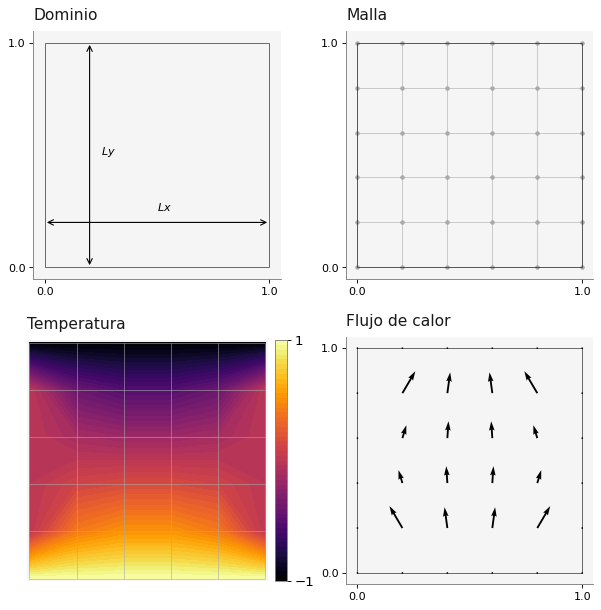
\includegraphics{05_Minimos_cuadrados_files/figure-pdf/cell-24-output-1.png}

\bookmarksetup{startatroot}

\chapter{Apéndice A: Deducción del
método.}\label{apuxe9ndice-a-deducciuxf3n-del-muxe9todo.}

Dado el conjunto de datos:

\begin{longtable}[]{@{}lllll@{}}
\toprule\noalign{}
\(x_0\) & \(x_1\) & \(x_2\) & \(\dots\) & \(x_N\) \\
\midrule\noalign{}
\endhead
\bottomrule\noalign{}
\endlastfoot
\(y_0\) & \(y_1\) & \(y_2\) & \(\dots\) & \(y_N\) \\
\end{longtable}

lo que en principio desearíamos es que se cumpliera que:

\[y_i = m x_i + b \;\; \text{para} \;\; i = 0, \dots, N \]

que es equivalente a

\[0 = m x_i + b - y_i\;\; \text{para} \;\; i = 0, \dots, N, \tag{A.1} \]

Pero la ecuación \((A.1)\) no se cumple en general, de tal manera que lo
que se pide es que las desviaciones de cada punto con respecto de la
recta sean pequeñas.

En el caso de este método, la desviación se define como la diferencia
del valor \(y_i\) con respecto de la recta elevada al cuadrado, es
decir: \((m x_i + b - y_i)^2\). Y para calcular la desviación global se
suman todas las diferencias, por lo que obtenemos:

\[
f(m,b) = \sum_{i=1}^{N} (m x_i + b - y_i)^2
\]

Observa que del lado derecho hemos puesto \(f(m,b)\) es decir, una
función que depende de la pendiente \(m\) y de la ordenada al origen
\(b\).

El valor de la función \(f\) (la desviación global) depende de \(m\) y
\(b\); entonces para encontrar los valores de \(m\) y \(b\) más
adecuados, debemos minimizar \(f\) con respecto a esas variables.

Recordando nuestras clases de cálculo, sabemos que para minimizar una
función, debemos calcular su derivada, igualarla a cero y resolver para
encontrar los puntos críticos (máximos y mínimos). En este caso, debemos
derivar con respecto a \(m\) y con respecto a \(b\), y luego resolver un
sistema de dos ecuaciones. Veamos como:

\[
\begin{eqnarray}
\dfrac{\partial f}{\partial m} & = & \dfrac{\partial}{\partial m} \left(\sum_{i=1}^{N} (m x_i + b - y_i)^2 \right) = 2 \sum_{i=1}^{N} x_i \big(m x_i + b - y_i\big) = 0 \tag{A.2}\\
\dfrac{\partial f}{\partial b} & = & \dfrac{\partial}{\partial b} \left(\sum_{i=1}^{N} (m x_i + b - y_i)^2 \right) = 2\sum_{i=1}^{N} \big(m x_i + b - y_i\big) = 0 \tag{A.3}\\
\end{eqnarray}
\]

De la ecuación \((A.3)\) tenemos que: \[
m \sum_{i=1}^{N} x_i + \sum_{i=1}^{N} b - \sum_{i=1}^{N} y_i = 0
\]

y despejando \(b\) obtenemos: \[
b = \underbrace{\dfrac{1}{N}\sum_{i=1}^{N} y_i}_{\bar{y}} - m \underbrace{\dfrac{1}{N} \sum_{i=1}^{N} x_i}_{\bar{x}} = \bar{y} - m \bar{x} \tag{A.4}
\]

Ahora sustituimos \((A.4)\) en \((A.2)\) y obtenemos:

\[
\sum_{i=1}^{N} x_i \big(m x_i + \bar{y} - m \bar{x} - y_i\big) = 0
\]

Ahora despejamos \(m\):

\[
m = \dfrac{\sum_{i=1}^{N} x_i(y_i - \bar{y})}{\sum_{i=1}^{N} x_i(x_i - \bar{x})} \tag{A.5}
\]

Las ecuaciones \((A.4)\) y \((A.5)\) proporcionan los valores de \(m\) y
\(b\) de un punto crítico de la función \(f(m,b)\). Falta demostrar que
ese punto crítico es un mínimo. Para ello se deben calcular las
derivadas segundas (\(\dfrac{\partial}{\partial^2 m}\),
\(\dfrac{\partial}{\partial^2 b}\),
\(\dfrac{\partial}{\partial m \partial b}\)) y ver que se cumplen los
criterios necesarios.



\end{document}
